
%%%%%%%%%%%%%%%%%%%%%%%% TEMPLATE INFO %%%%%%%%%%%%%%%%%%%%%%%%%%%%%%
%:     Template Name = cpe-thesis-th
%:     Version Name  = th-vectier-1.1
%:     Created by:
%:       - Peerapon Siripongwutikorn (peerapon@cpe.kmutt.ac.th), 2016-2020
%:     Modified by:
%:       - Thanin Srithai (thanin.srithai2@mail.kmutt.ac.th), 2021-2022
%:       - Jatetanan Kanchanawat (jate@jate-koh.com), 2024
%:       - Vectier (support@vectier.com), 2024
%:
%: This is a LaTeX template for use in CPE, KMUTT report and thesis.
%%%%%%%%%%%%%%%%%%%%%%%%%%%%%%%%%%%%%%%%%%%%%%%%%%%%%%%%%%%%%%%%%%%%%
%: Instructions:
%: Run at the command line, run: xelatex <filename>.tex
%: Note: Run a few times to generate the output pdf file
%:
%%%%%%%%%%%%%%%%%%%%%%%%%% FILE INFO %%%%%%%%%%%%%%%%%%%%%%%%%%%%%%%%
%:     File name = report.tex
%:     Authors:
%:       - Jatetanan Kanchanawat
%:       - Krid Hepakrone
%:
%%%%%%%%%%%%%%%%%%%%%%%%%%%%%%%%%%%%%%%%%%%%%%%%%%%%%%%%%%%%%%%%%%%%%

%%%%%%%%%%%%%%%%%%%%%%%%%% REPORT START %%%%%%%%%%%%%%%%%%%%%%%%%%%%%
\documentclass[12pt,one side,openright,a4paper]{cpe-thesis-th}

%%%%%%%%%%%%%%%%%%%%%% Packages and Configs %%%%%%%%%%%%%%%%%%%%%%%%%

\usepackage{color}
\usepackage{pgfgantt}                   % Gantt chart
\usepackage{polyglossia}
\usepackage{caption}                    % Figures and tables captions

\usepackage{etoolbox}                   % Patching commands for macros creating i.e. preto
\usepackage{longtable}                  % Long continuous table
\usepackage{ragged2e}                   % Forcing figure
\usepackage{float}                      % ER and checkmark
\usepackage{tikz}                       % Drawing graphs and symbols
\usepackage{subfig}                     % Subfigures
\usepackage{keyval}                     % Subfigures alignment
\usepackage[export]{adjustbox}          % Subfigures aLignment
\usepackage{cleveref}                   % Clever label references

\usepackage{lmodern}
\usepackage{listings}                   % Listings as code blocks
\usepackage{packages/listings-golang}   % Listings support for Golang
\usepackage{packages/listings-yaml}     % Listing support for YAML

%: Biblatex for managing bibliography; instead of using old \bibliography{}
%: NOTE: Biblatex define typesetting onto compilation cache.
%: So recompile from scratch (Remove aux and bbl file and recompile)
%: Everytime you stopped using biblatex

\usepackage[
    backend=biber,      % Biber or Bibtex
    style=ieee,         % Bib standard
    sorting=none,       % Sort by appearance in paper
    % sorting=ynt,       % Sort by year, name...
    % sortcites=true,    % Some other  example options ...
    dateabbrev=true,
    urldate=long,
    block=none,
    indexing=false,
    citereset=none,
    isbn=true,
    url=true,
    doi=true,           % Prints DOI
    natbib=true         % if you need Natbib functions
]{biblatex}


%%%%%%%%%%%%%%%%%% Custom Macros & Settings %%%%%%%%%%%%%%%%%%%%%%%
%: From this part to \begin{document}
%: Do not modify unless you know what you are doing...

%%%%%%%%%%%%%%%%%%%%%%%%%%%%%%%%%
%%%%%%% Biblatex macro %%%%%%%%%%

%: Setup URL access date string
\DefineBibliographyStrings{english}{%
    urlseen = {accessed}
}

%: Reference bib files
%: Make sure you reference correct bib file...
\addbibresource{bib/codern.bib}

%%%%%%%%%%%%%%%%%%%%%%%%%%%%%%%%%
%%%%%%%%% Font settings %%%%%%%%%

%: Define 1st and 2nd language
\setdefaultlanguage{thai}
\setotherlanguage{english}

%: Uncomment following to used Laksaman
%: which is equivalent of Sarabun
% \setmainfont[
%     Scale=1.0,
%     LetterSpace=0,
%     WordSpace=1.0,
%     FakeStretch=1.0,
%     Mapping=tex-text
% ]{Laksaman:script=thai}
% \newfontfamily\thaifont[
%     Scale=1.0,
%     LetterSpace=0,
%     WordSpace=1.0,
%     FakeStretch=1.0,
%     Mapping=tex-text
% ]{Laksaman:script=thai}
% \newfontfamily\thaifonttt{Tlwg Typist:script=thai}

%: Uncomment to use actual Sarabun (font file required)
\newfontfamily\thaifont[Script=Thai,Scale=1.23]{THSarabunNew.ttf}[
    Path=fonts/,
    Extension=.ttf,
    BoldFont=*-Bold,
    ItalicFont=*-Italic,
    BoldItalicFont=*-BoldItalic,
]
\defaultfontfeatures{Mapping=tex-text,Scale=1.23,LetterSpace=0.0}
\setmainfont[Scale=1.23,LetterSpace=0,WordSpace=1.0,FakeStretch=1.0,Mapping=tex-text]{THSarabunNew.ttf}[
    Path=fonts/,
    Extension=.ttf,
    BoldFont=*-Bold,
    ItalicFont=*-Italic,
    BoldItalicFont=*-BoldItalic,
]

%: Set linebreak to Thai
\XeTeXlinebreaklocale "th"
\XeTeXlinebreakskip = 0pt plus 0pt
\emergencystretch=10pt

%: Define fonts for code blocks
\newfontfamily\codefont[Scale=0.9]{CourierPrime.ttf}[
    Path=fonts/,
    Extension=.ttf,
    BoldFont=*-Bold,
    ItalicFont=*-Italic,
    BoldItalicFont=*-BoldItalic,
]

%%%%%%%%%%%%%%%%%%%%%%%%%%%%%%%%%
%%%%%%%% Margin settings %%%%%%%%
%\linespread{1.6} % Double-spaced
%\oddsidemargin    0.5in
%\evensidemargin   0.5in

%%%%%%%%%%%%%%%%%%%%%%%%%%%%%%%%%
%%%%%% Paragraph Settings %%%%%%%
\linespread{1.15}

\newcommand{\thaijustify}[1]{%
  % \ifnum\value{isfigure}=0
  %   \newline % If counter is set, no newline
  % \fi
  \par\hspace{30pt}\justifying
  #1
  % \vspace{1mm}
  % \setcounter{isfigure}{0}%
}

\newcommand{\thaicaption}[1]{%
  % \ifnum\value{isfigure}=0
  %   \newline % If counter is set, no newline
  % \fi
  \par\justifying
  #1
  % \vspace{1mm}
  % \setcounter{isfigure}{0}%
}

%%%%%%%%%%%%%%%%%%%%%%%%%%%%%%%%%
%%%%%% Caption settings %%%%%%%%%
%: Define how the captions of each report
%: element are formatted.

\captionsetup[table]{
    format=hang,
    labelfont=bf,
    position=top,
    labelsep=space,
    justification=justified,
    singlelinecheck=true
}
\captionsetup[figure]{
    format=hang,
    labelfont=bf,
    position=bottom,
    labelsep=space,
    justification=justified,
    singlelinecheck=true
}
\captionsetup[subfloat]{
    format=hang,
    labelfont=bf,
    labelformat=simple,
    labelsep=period,
    justification=justified,
    singlelinecheck=true
    %listofformat=subparens
}
\captionsetup[lstlisting]{
    format=hang,
    labelfont=bf,
    position=top,
    labelsep=space,
    justification=justified,
    singlelinecheck=true,
    skip=10pt
}
%%%%%%%%%%%%%%%%%%%%%%%%%%%%%%%%%
%%%%%%% Numbering styling %%%%%%%
% Enumerate using arabic numbers
\renewcommand{\labelenumii}{\arabic{enumi}.\arabic{enumii}}
\renewcommand{\labelenumiii}{\arabic{enumi}.\arabic{enumii}.\arabic{enumiii}}
\renewcommand{\labelenumiv}{\arabic{enumi}.\arabic{enumii}.\arabic{enumiii}.\arabic{enumiv}}

%%%%%%%%%%%%%%%%%%%%%%%%%%%%%%%%%
%%%%%% Subfigure settings %%%%%%%

%\renewcommand{\subfigtopskip}{10pt}
%\renewcommand{\subfigbottomskip}{-5pt}
%\renewcommand{\subfigcapskip}{-6pt} %vertical space between caption
%                                    %and figure.
%\renewcommand{\subfigcapmargin}{0pt}

% Use thai alphabets for captions
\renewcommand{\thesubfigure}{\thalph{subfigure}}

%%%%%%%%%%%%%%%%%%%%%%%%%%%%%%%%
%%%%%%% Tikz Settings %%%%%%%%%%
%: Tikz is used for drawing simple edge and node graph
%: Import shapes for usage
\usetikzlibrary{er, positioning, shapes.geometric, arrows}

%: Define checkmark symbol
\def\checkmark{\tikz\fill[scale=0.4](0,.35) -- (.25,0) -- (1,.7) -- (.25,.15) -- cycle;}

%%%%%%%%%%%%%%%%%%%%%%%%%%%%%%%%
%%%%%% Listings Settings %%%%%%%%
%: Listings is used for displaying the program or
%: codes in reports as statement

%: Define text color for code blocks
\definecolor{dkgreen}{rgb}{0,0.6,0}
\definecolor{gray}{rgb}{0.5,0.5,0.5}
\definecolor{mauve}{rgb}{0.58,0,0.82}

%: Define code blocks settings
\lstset{
    frame=tb,
    language=Golang,
    aboveskip=3mm,
    belowskip=3mm,
    showstringspaces=false,
    columns=flexible,
    basicstyle={\small\codefont},
    numbers=left,
    numberstyle=\small\color{gray},
    keywordstyle=\color{blue},
    commentstyle=\color{dkgreen},
    stringstyle=\color{mauve},
    breaklines=false,
    breakatwhitespace=false,
    tabsize=3
}

%%%%%%%%%%%%%%%%%%%%%%%%%%%%%%%%%
%%%%%%%%%% Math macro %%%%%%%%%%%
%: Fraction settings
\renewcommand{\topfraction}{0.85}
\renewcommand{\textfraction}{0.1}

%: Define theorem and proof
\newtheorem{theorem}{Theorem}
\newtheorem{lemma}{Lemma}
\newtheorem{corollary}{Corollary}

\def\QED{\mbox{\rule[0pt]{1.5ex}{1.5ex}}}
\def\proof{\noindent\hspace{2em}{\itshape Proof: }}
\def\endproof{\hspace*{\fill}~\QED\par\endtrivlist\unskip}

%\newenvironment{proof}{{\sc Proof:}}{~\hfill \blacksquare}
%% The hyperref package redefines the \appendix. This one
%% is from the dissertation.cls
%\def\appendix#1{\iffirstappendix \appendixcover \firstappendixfalse \fi \chapter{#1}}
%\renewcommand{\arraystretch}{0.8}
%%%%%%%%%%%%%%%%%%%%%%%%%%%%%%%%%

%%%%%%%%%%%%%%%%%%%%% Report Definitions %%%%%%%%%%%%%%%%%%%%%%%%%%
%: Customize below to suit your needs
%: The optional ones can be left blank.

%: First line of title
\def\disstitleone{Coding Platform}
\def\thaidisstitleone{Coding Platform}

%: Second line of title
\def\disstitletwo{Code Autograding System for C/C++ Program Verification}
\def\disstitlethree{using Golang and Containerization Technology}
\def\thaidisstitletwo{ระบบตรวจงานเขียนชุดคำสั่งโปรแกรมภาษาคอมพิวเตอรสำหรับการตรวจโปรแกรมภาษา }
\def\thaidisstitlethree{C หรือ C++ โดยภาษาคอมพิวเตอร์ Golang และเทคโนโลยี Containerization}

%: Authors
\def\dissauthor{Mr. Krid Heprakrone}          % 1st member
\def\thaidissauthor{นายกฤษฎิ์ เฮ่ประโคน}
\def\dissauthortwo{Mr. Jatetanan Kanchanawat} % 2nd member (optional)
\def\thaidissauthortwo{นายเจตนันท์ กาญจนวัฒน์}
\def\dissauthorthree{Ms. Pimmada Laisuan}     % 3rd member (optional)
\def\thaidissauthorthree{นางสาวพิมพ์มาดา ไล่สวน}

%: The degree that you're pursuing..
\def\dissdegree{Bachelor of Engineering}        % Name of the degree
\def\thaidissdegree{วิศวกรรมศาสตรบัณฑิต}
\def\dissdegreeabrev{B.Eng}                     % Abbreviation of the degree
\def\dissyear{2023}                             % Year of submission
\def\thaidissyear{2566}                         % Year of submission (B.E.)

%: Your project or independent study's committee
%: Example of appropriate advisor/committee name entries
%: Example 1: Assoc. Prof. Natasha Dejdumrong, D. Tech. Sci.
%: Example 2: Asst. Prof. Dr.Ing Priyakorn Pusawiro
%: Example 3: Jaturon Harnsomburana, Ph.D.

%: Advisors
\def\dissadvisor{Assoc. Prof. Natasha Dejdumrong, D. Tech. Sci.} % Advisor
\def\thaidissadvisor{รศ.ดร.ณัฐชา เดชดำรง}

%: Note: Leave the following empty if you have no co-advisor
\def\disscoadvisor{} % Co-advisor (optional)
\def\disscoadvisortwo{} % Co-advisor (optional)
\def\thaidisscoadvisor{}
\def\thaidisscoadvisortwo{}

%: Committee Members
%: Note: Leave the following empty if no person is in that position
\def\disscommitteetwo{Asst. Prof. Dr.Ing Priyakorn Pusawiro} % 3rd committee member
\def\disscommitteethree{Asst. Prof. Rajchawit Sarochawikasit} % 4th committee member (optional)
\def\disscommitteefour{Jaturon Harnsomburana, Ph.D.} % 5th committee member (optional)

%: Project Type
\def\worktype{Project}          % Project or Independent study
\def\thaiworktype{ปริญญานิพนธ์}    %  Project or Independent study
\def\disscredit{3}              % 3 credits or 6 credits

%: Department Information
\def\fieldofstudy{Computer Engineering}
\def\department{Computer Engineering}
\def\faculty{Engineering}
\def\thaifieldofstudy{วิศวกรรมคอมพิวเตอร์}
\def\thaidepartment{วิศวกรรมคอมพิวเตอร์}
\def\thaifaculty{วิศวกรรมศาสตร์}

%%%%%%%%%%%%%%%%% Front Page + Signature Page %%%%%%%%%%%%%%%%%%
\begin{document}

\pdfstringdefDisableCommands{
  \let\MakeUppercase\relax
}

\begin{center}
  
\includegraphics[width=2.8cm]{./figure/logo02.jpg}
\end{center}
\vspace*{-1cm}

\maketitlepage
\makesignaturepage

%%%%%%%%%%%%%%%%%%%%%% English abstract %%%%%%%%%%%%%%%%%%%%%%%%
\abstract
Proficiency in computer programming is a vital skill in computer science, leading to a surge in student enrollment for programming courses. However, the effectiveness of teaching programming diminishes as class sizes increase, and instructors find it challenging to manually assess each student's assignments promptly. To address this issue, we propose developing a software solution, Coding Platform, a code auto-grading system written in Golang utilizing containerization technology, designed to automate and streamline the grading process. This software aims to evaluate student submissions against predefined test cases, measure resource usage efficiency, and instantly provide feedback and scores. This reduces the burden on instructors and fosters a competitive and engaging learning environment. The platform also maintains a comprehensive record of student performance, aiding both instructors in refining their teaching methods and students in showcasing their achievements. The software had been deployed for its intended use and has, ever since, been tested by both instructors and students alike, in classroom environments and competitive scenes like BangMod Hackathon 2024. Consequently, this grading system has been updated and refined actively as users' bug reports and feature requests are always addressed followed by various updates, fixes, and patches. Overall, the software was very well-received, with survey results averaging an overall score of 8 and good user ratings on the software's functionalities and performance.

\justifying
\begin{tabular*}{\textwidth}{@{}lp{0.8\textwidth}}
  \textbf{Keywords}: & Programming Education / Student Assessment / Golang / Containerization
\end{tabular*}
\vspace{1mm}
\endabstract

%%%%%%%%%%%%%%%%%%%%%%%% Thai abstract %%%%%%%%%%%%%%%%%%%%%%%%%

\thaiabstract
\justifying
ความเชี่ยวชาญในการเขียนโปรแกรมคอมพิวเตอร์เป็นทักษะสำคัญในวิทยาการคอมพิวเตอร์ ส่งผลให้ในช่วงมาหลังมีนักศึกษาหันมาสนใจและลงทะเบียนในหลักสูตรการเขียนโปรแกรมเพิ่มมากขึ้น ส่งผลให้ประสิทธิภาพของการสอนการเขียนโปรแกรมจะลดลงเนื่องจากจำนวนผู้เรียนเพิ่มมากขึ้น อาจารย์ผู้สอนพบว่าการประเมินงานมอบหมายของนักเรียนแต่ละคนด้วยตนเองเป็นเรื่องท้าทาย เพื่อแก้ไขปัญหานี้ คณะผู้จัดทำเสนอเเนวทางเเก้ไขปัญหาในรูปเเบบของซอฟต์แวร์ชื่อ Coding Platform ขี้นมาด้วยภาษา Golang และออกแบบด้วยเทคโนโลยี Containerization ระบบซอฟต์แวร์ดังกล่าวจะเป็นระบบสำหรับตรวจโปรแกรมที่นักศึกษาเขียนส่งมาในระบบ แล้วให้ผลตรวจในทันที ซอฟต์แวร์ดังกล่าวจะตรวจและประเมินงานที่ผู้ใช้ส่งมาเทียบกับกรณีทดสอบที่กำหนดไว้ล่วงหน้าและวัดประสิทธิภาพการใช้ทรัพยากรของตัวโปรแกรม จากนั้นจะนำผลตรวจด้งกล่าวไปแสดงในทันที สิ่งนี้ไม่เพียงแต่ช่วยลดภาระของผู้สอนเท่านั้น แพลตฟอร์มดังกล่าวยังรักษาบันทึกผลเเละข้อมููลการใช้งานของผู้ใช้อย่างครอบคลุมเพื่อนำมาเป็นข้อมูลให้อาจารย์ผู้สอนปรับปรุงวิธีการสอนของตน และจัดแสดงความสำเร็จของนักศึกษาเพื่อส่งเสริมสภาพแวดล้อมการเรียนรู้ที่มีการแข่งขันและการมีส่วนร่วม โดยซอฟต์แวร์ดังกล่าวได้ถูกติดตั้งใช้งานแล้ว ซึ่งได้เปิดโอกาสให้ผู้ใช้ทั้งอาจารย์ผู้สอนและนักศึกษาได้ลองใช้งาน ทั้งในห้องเรียนและกิจกรรมวิชาการอย่าง BangMod Hackathon 2024 รวมไปถึงให้ผู้ใช้ได้วิจารณ์และให้คำติชมเพื่อที่จะได้นำไปปรับปรุงและแก้ไขข้อผิดพลาด ซึ่งส่งผลให้ซอฟต์แวร์นั้นได้รับผลตอบรับที่ดีจากผู้ใช้มากมายในแบบประเมินผล ดัวยคะแนนเฉลี่ยของภาพรวมซอฟต์แวร์ที่ 8 คะแนน พร้อมผลคะแนนและคำชมเชยมากมายในด้านความสามารถและประสิทธิภาพการทำงานของซอฟต์แวร์

\justifying
\begin{tabular*}{\textwidth}{@{}lp{0.8\textwidth}}
  & \\
  \textbf{คำสำคัญ}: & รายวิชาการสอนเขียนโปรแกรม / การวัดและประเมินผลนักศึกษา / ภาษา Golang / เทคโนโลยี Containerization
\end{tabular*}
\vspace{1mm}
\endabstract

%%%%%%%%%%%%%%%%%%%%%%%%% Acknowledgments %%%%%%%%%%%%%%%%%%%%%%
\preface
โครงงานพัฒนาโปรแกรม/แอปพลิเคชัน/เว็บแอปพลิเคชัน สำหรับตรวจงานและข้อสอบในรายวิชาการเรียนการสอนเขียนโปรแกรมภาษาคอมพิวเตอร์ หรือ Coding Platform สามารถบรรลุเป้าหมายไปได้ด้วยดี ทางคณะผู้จัดทำต้องขอขอบคุณผู้สนับสนุนทุกท่านที่ให้การช่วยเหลือในด้านต่าง ๆ ขอขอบคุณ รศ.ดร.ณัฐชา เดชดำรง ที่มาเป็นอาจารย์ที่ปรึกษาโครง สละเวลาในการให้ความรู้ พร้อมให้คำแนะนำตลอดการพัฒนาทั้งโครงงาน ขอขอบคุณภาควิชาวิศวกรรมคอมพิวเตอร์ คณะวิศวกรรมศาสตร์ มหาวิทยาลัยเทคโนโลยีพระจอมเกล้าธนบุรี ที่ให้การส่งเสริมและสนับสนุนทางคณะผู้จัดทำ ตลอดจนเอื้อเฟื้อสถานที่และอุปกรณ์สำหรับการพัฒนาโครงงาน ขอขอบคุณนักศึกษาชั้นปีที่หนึ่งและสอง ที่เรียนวิชา CPE222 Algorithm Design, CPE100 Computer Programming for Engineers, CPE112 Programming with Data Structures ปีการศึกษาพุทธศักราช 2566 รวมไปถึงนักเรียนชั้นมัธยมศึกษาตอนปลายที่เข้าร่วมโครงการกิจกรรมการเเข่งขันเขียนโปรเเกรมคอมพิวเตอร์ Bangmod Hackathon 2024 ที่จัดขึ้นในปีการศึกษาเดียวกัน ที่สละเวลามาทดลองใช้ซอฟต์เเวร์ต้นแบบ พร้อมทั้งแสดงความเห็น ให้่ข้อเสนอแนะ ให้คำติชมที่ล้วนแต่เป็นข้อมูลอันเป็นประโยชน์ ที่สามารถนำมาใช้ในการพัฒนาซอฟต์แวร์

%%%%%%%%% Table of Contents, List of Figures/Tables %%%%%%%%%%%%
%: The three commands below automatically generate the table
%: of content, list of tables, list of figures, and list of listings

%: Appendices or Appendix
%: If you have more than one appendix, use `Appendices`
\def\appendixnames{Appendices}

\tableofcontents
\listoftables
\listoffigures

%%%%%%%%%%%%%%%%%%%%%%%% List of codes %%%%%%%%%%%%%%%%%%%%%%%%%
%: Command below automatically will generate the table
%: for listing 'lst' package listings

\listofprograms

%%%%%%%%%%%%%%%%%%%%%%%% List of symbols %%%%%%%%%%%%%%%%%%%%%%%
%: You have to add this manually...

% \listofsymbols
% \newline\justifying{
% \begin{tabular}{@{}p{0.07\textwidth}p{0.7\textwidth}p{0.1\textwidth}}
% \textbf{สัญลักษณ์} & & \textbf{หน่วย} \\[0.2cm]
%     $\alpha$ & Test variable\hfill & m$^2$ \\
%     $\lambda$ & Interarival rate\hfill &  jobs/second\\
%     $\mu$ & Service rate\hfill & jobs/second\\
% \end{tabular}
% }

%%%%%%%%%%%%%%%%%%%%% List of vocabs & terms %%%%%%%%%%%%%%%%%%%
%: You also have to add this manually...

\newcommand{\tableraglf}[1]{\RaggedRight{#1}}
\listofvocab
\begin{flushleft}
  \begin{tabular}{@{}p{2in}@{\hspace{0.1in}=\extracolsep{0.2in}}p{4in}}
    % Application / แอปพลิเคชัน & \tableraglf{โปรแกรมหรือซอฟต์แวร์คอมพิวเตอร์สำหรับรูปแบบหนึ่งรูปแบบใด~\cite{oxfordlearner} หรือโปรแกรมซอฟต์แวร์ที่ทำงานอยู่บนระบบสารสนเทศ~\cite{cnssi4009}} \\
    % Code / โค้ด & \tableraglf{คำสั่งคอมพิวเตอร์และคำจำกัดความของข้อมูลที่แสดงเป็นภาษาโปรแกรมหรือในรูปแบบเอาต์พุตโดยแอสเซมเบลอร์ คอมไพลเลอร์ หรือนักแปลอื่น ๆ~\cite{cnssi4009}} \\
    % Source Code / รหัสต้นฉบับ / ซอร์สโค้ด / รหัสต้นทาง & \tableraglf{ชุดของข้อความที่ถูกเขียนขึ้นด้วยภาษาโปรแกรมที่มนุษย์สามารถอ่านและเข้าใจได้~\cite{linfo04}} \\
    PDF                                    & \tableraglf{ย่อมาจาก Portable Document File แปลว่ารูปแบบไฟล์เอกสารที่สามารถเคลื่อนย้ายไปมาได้อย่างสะดวก}                                                                                                           \\ %~\cite{nist8219, nistsp800pdf}
    UI / ส่วนประสานงานผู้ใช้                   & \tableraglf{ย่อมาจาก User Interface ในภาษาอังกฤษ หมายถึงส่วนที่ให้ผู้ใช้งานสามารถโต้ตอบกับการใช้งานผลิตภัณฑ์ได้ ซึ่งจะมุ่งเน้นไปที่เรื่องของหน้าตา การออกแบบ เช่น หน้าจอ แพลตฟอร์ม เมนู ฟอร์ม}                                          \\ %~\cite{nistsp800ui} ~\cite{dmit19ui}
    UX / ประสบการณ์ของผู้ใช้                   & \tableraglf{ย่อมาจาก User Experience ในภาษาอังกฤษ ประสบการณ์ของผู้ใช้งานในด้านความรู้สึกที่ตอบสนองต่อการใช้งานผลิตภัณฑ์ หรือระบบต่าง ๆ ยกตัวอย่างเช่น ความสะดวกสบาย ใช้งานง่าย ความสนุกสนาน}                                     \\ %~\cite{dmit19ui} ~\cite{nistsp800ui}
    MD                                     & \tableraglf{ย่อมาจากคำว่า Markdown ซึ่งเป็นภาษา Markup ที่เรียบง่าย ที่มีความคล้ายคลึงกับภาษามนุษย์ โดยหลักการเขียนอิงตามแบบแผนข้อความธรรมดา (plain text) ที่ผ่านการทดสอบและรวบรวมเป็นมาตรฐาน อิงจากข้อมูลที่เก็บเป็นช่วงเวลา 40 ปีที่ผ่านมา} \\ %~\cite{atwoodmd}
    Compiler / คอมไพลเลอร์                  & \tableraglf{ซอฟต์แวร์ที่แปลภาษาโปรแกรมคอมพิวเตอร์ระดับสูงที่คนเข้าใจ ให้อยู่ในรูปแบบภาษาที่คอมพิวเตอร์สามารถดำเนินการได้}                                                                                                     \\ %~\cite{astmcompiler}
    % Inherit (Object) / สืบทอด (วัตถุ) & \tableraglf{ในเชิงการเขียนโปรแกรมเชิงวัตถุ หมายถึง (วัตถุ) สืบทอดคุณสมบัติจากอีกวัตถุหนึ่ง} \\
    % Implements (Object) / ปฏิบัติตาม (วัตถุ) & \tableraglf{ในเชิงการเขียนโปรแกรมเชิงวัตถุ หมายถึง การปฏิบัติตามคุณสมบัติหรือกฏเกณฑ์ของอีกวัตถุ (โดยเฉพาวัตถุประเภท Interface)}  \\
    Run (Program) / รัน (โปรแกรม)           & \tableraglf{ในเชิงของการเขียนโปรแกรมและซอฟต์แวร์ แปลว่าการนำชุดคำสั่งหรือชุดของโค้ดหรือโปรแกรม ไปเปิดใช้งาน}                                                                                                            \\
    Grader / เกรดเดอร์                      & \tableraglf{ตัวโปรแกรมหรือซอฟต์แวร์ที่จะเอาโปรแกรมที่เขียนมาไปลองรันทดสอบ แล้วเทียบเทสเคสกับค่าผลลัพธ์ที่แสดงออก เพื่อตัดสินและประเมินความถูกต้องของโปรแกรม}                                                                     \\
    Test Case / กรณีทดสอบโปรแกรม / เทสเคส   & \tableraglf{ชุดของค่าอินพุต เงื่อนไขเบื้องต้นในการดำเนินการ ผลลัพธ์ที่คาดหวัง และเงื่อนไขหลังการดำเนินการ พัฒนาขึ้นสำหรับ วัตถุประสงค์เฉพาะหรือเงื่อนไขการทดสอบ}                                                                        \\ %~\cite{istqb}}
    Assignment / โจทย์ปัญหา / ข้อสอบ / การบ้าน & ในรายงานนี้ หมายถึงโจทย์ปัญหาที่เป็นปัญหาในเชิงอัลกอริทึม ที่จะต้องแก้โจทย์ด้วยการเขียนโปรแกรมภาษาคอมพิวเตอร์ป้อนเข้าไปเพื่อให้คอมพิวเตอร์แก้ไขปัญหาให้                                                                                 \\
    Memory Limit / ขีดจำกัดหน่วยความจำ          & \tableraglf{ปริมาณทรัพยากรการคำนวณ ที่โปรแกรมสามารถใช้ได้ ในการประมวลผลหาคำตอบของโจทย์ปัญหาเชิงโปรแกรม}                                                                                                            \\
    Time Limit / ระยะเวลาจำกัด               & \tableraglf{ระยะเวลามากที่สุด ที่โปรแกรมใช้ได้ในการประมวลผล หาคำตอบสำหรับโจทย์ปัญหาเชิงโปรแกรม}                                                                                                                      \\
  \end{tabular}
\end{flushleft}

%\setlength{\parskip}{1.2mm}

%%%%%%%%%%%%%%%%%%%%%%% Main body %%%%%%%%%%%%%%%%%%%%%%%%%%%%%%

\chapter{บทนำ}
\section{ที่มาและความสำคัญ}
\thaijustify{
  ทักษะการเขียนโปรแกรมคอมพิวเตอร์เป็นทักษะที่สำคัญสำหรับวิชาชีพในสาขาวิทยาการคอมพิวเตอร์ เป็นเหตุให้นักศึกษาจำนวนมากหันมาสมัครหรือลงวิชาเขียนโปรแกรมคอมพิวเตอร์เพิ่มมากขึ้น ทำให้การเรียนการสอนวิชาเขียนโปรแกรมคอมพิวเตอร์มีประสิทธิภาพที่ต่ำลงเพราะจำนวนผู้เรียนมากขึ้น อาจารย์ผู้สอนไม่สามารถจะดูแลนักศึกษาได้ครบทุกคน การตรวจงานและให้คะแนนใช้ระยะเวลานาน เพราะอาจารย์ผู้สอนจะต้องนำไฟล์งานของนักศึกษามาตรวจทีละไฟล์ อีกทั้งยังมีโอกาสเกิดข้อผิดพลาดในการตรวจอีกด้วย
}
\thaijustify{
  จากปัญหาดังกล่าว กลุ่มผู้จัดทำได้มีแนวทางแก้ปัญหาด้วยการสร้างเป็นโครงงานพัฒนาซอฟต์แวร์ Coding Platform เพื่อให้อาจารย์ผู้สอนได้นำไปใช้เป็นเครื่องมือช่วยตรวจงานของนักศึกษาโดยอัตโนมัติ ด้วยแนวทางนี้อาจารย์ผู้สอนจะได้ไม่ต้องทุ่มเททรัพยากรและเวลาไปกับการตรวจการบ้าน แล้วสามารถที่จะทุ่มเทไปยังงานในด้านการสอน และพัฒนาคุณภาพการเรียนการสอนในรายวิชา
}
\thaijustify{
  โดยซอฟต์แวร์จะนำไฟล์ชุดคำสั่งที่นักศึกษาส่งเข้ามาในระบบ มาตรวจสอบความถูกต้องจากชุดข้อมูลทดสอบ (Test Case) ที่อาจารย์ผู้สอนได้กำหนดไว้ในโจทย์แต่ละข้อ จากนั้นนำไปวัดและประเมินประสิทธิภาพของการใช้ทรัพยากรของโปรแกรมเช่น ระยะเวลาหรือปริมาณหน่วยความจำที่ถูกโปรแกรมใช้ในประมวลผลหาคำตอบ หลังจากตรวจเสร็จ ระบบจะบันทึกผลลัพธ์และแสดงผลลัพธ์การตรวจให้นักศึกษาได้เห็นในทันที เพื่อเสริมสร้างความสนุกสนาน การแข่งขันและส่งเสริมนักศึกษาให้พัฒนาตนเอง อีกทั้งประวัติการใช้งาน งานทั้งหมดที่นักศึกษาได้ส่ง จะถูกนำไปเก็บไว้ในระบบฐานข้อมูลผู้ใช้อีกด้วย เพื่อให้อาจารย์ผู้สอนไปใช้การปรับปรุงหรือพัฒนาการสอนต่อๆ ไป หรือเพื่อให้นักศึกษานำเอาผลงานที่ได้ทำในระบบ ไปยื่นประกอบกับพอร์ทโฟลิโอในฐานะหลักฐานและผลงานความสำเร็จ
}

\section{วัตถุประสงค์}
ทางกลุ่มคณะผู้จัดทำ ได้ดำเนินโครงการพัฒนาซอฟต์เเวร์ดังกล่าว ด้วยวัตถุประสงค์ดังต่อไปนี้
\begin{enumerate}
  \item เพื่อนำความรู้การบริหารจัดการงานด้านซอฟต์แวร์จากวิชาวิศวกรรมซอฟต์เเวร์ มาประยุกต์ใช้กับการทำงาน
  \item เพื่อสร้างโอกาสทดลอง ออกแบบและสร้างซอฟต์แวร์ขนาดใหญ่ ในระดับมืออาชีพ
  \item เพื่อนำหลักการออกเเบบในทางวิศวกรรม ที่เรียนมาจากรายวิชาของภาควิชาวิศวกรรมคอมพิวเตอร์ มาออกเเบบสร้างระบบซอฟต์เเวร์ที่มั่นคงและยั่งยืน
  \item เพื่อช่วยอาจารย์ผู้สอนตรวจงาน วัดและประเมินแบบฝึกหัด การบ้าน หรือข้อสอบนักศึกษาในรายวิชาการเขียนโปรแกรมคอมพิวเตอร์
  \item เพื่อช่วยคณะกรรมการหรือคณะผู้จัดการแข่งขันเขียนโปรแกรม ตรวจข้อสอบในโครงการแข่งขันเขียนโปรแกรมคอมพิวเตอร์ที่จัดขึ้นในภาควิชา
  \item เพื่อเก็บข้อมูลการเรียนการสอน ทั้งโจทย์ปัญหาและการบ้านที่นักศึกษาได้ทำ และผลสอบของนักศึกษาเข้าฐานข้อมูลผู้ใช้ เพื่อให้อาจารย์ผู้สอนไปใช้อ้างอิงและพัฒนาคุณภาพการสอนต่อๆ ไป
\end{enumerate}

\section{ขอบเขตของโครงงาน}
\begin{enumerate}
  \item ซอฟต์แวร์รองรับการแสดงผลเป็นภาษาอังกฤษ
  \item ซอฟต์แวร์เน้นการใช้งานบนหน้าจอ Desktop
  \item มีระบบลงทะเบียนหรือยืนยันตัวตนผู้ใช้ (User registration and Authentication System)
  \item มีหน้าแสดงโจทย์ปัญหา ให้นักศึกษา/ผู้เข้าร่วมการแข่งขัน/ผู้ใช้ทั่วไปดู
        \begin{enumerate}
          \item รองรับการแสดงโจทย์แบบ Markdown, ไฟล์ PDF, และรูปภาพ
        \end{enumerate}
  \item มีแผงสำหรับเขียนโปรแกรมหรือแก้ไขโค้ด (Built-in code editor) คู่กับโจทย์ ในหน้าแสดงโจทย์
  \item มีระบบคอมไพลเลอร์สำหรับรันโปรแกรมที่ส่งเข้ามา (Built-in code compiler)
        \begin{enumerate}
          \item รองรับภาษา C และ C++ เป็นหลัก
          \item คอมไพลเลอร์รันโปรแกรมที่ส่งเข้ามา เพื่อตรวจสอบความถูกต้องในขั้นตรวจงาน (Grading)
          \item คอมไพลเลอร์รันโปรแกรมเพื่อแสดงผลลัพธ์ให้นักศึกษาดู ในหน้าแผงเขียนโปรแกรมเพื่อตรวจโปรแกรมก่อนส่ง (debugging)
        \end{enumerate}
  \item มีระบบตรวจและประเมินโค้ดที่ได้ส่งเข้ามา (Automatic grader and Evaluation) โดยประเมินจาก
        \begin{enumerate}
          \item ความถูกต้อง (Correction) โดยเทียบชุดข้อมูลส่งออก (Output) ของโปรแกรมกับชุดข้อมูลทดสอบ (Test case) ที่กำหนดไว้ในโจทย์ข้อนั้นๆ
          \item ประสิทธิภาพ (Performance) ประเมินโดยเทียบกับตัวแปร/ตัวชี้วัด (Metrics) ต่อไปนี้
                \begin{itemize}
                  \item ระยะเวลาที่ใช้ในการหาคำตอบ (Runtime)
                  \item ปริมาณหรือจำนวนหน่วยความจำที่โปรแกรมใช้ (Memory usage)
                \end{itemize}
        \end{enumerate}
  \item มีระบบห้องเรียน/กลุ่มเรียน/กลุ่มงาน (Class/Group/Workspace) ตามรายวิชาสำหรับเก็บโจทย์
  \item มีแผงควบคุมสำหรับอาจารย์/ผู้สอน/แอดมิน (Admin/Instructor/Lecturer Dashboard) โดยในแผงควบคุมดังกล่าวอาจารย์/ผู้สอน/แอดมินสามารถ
        \begin{enumerate}
          \item สร้าง/แก้ไข/ลบ แอคเคาน์นักศึกษา/ผู้เข้าร่วมการแข่งขัน/ผู้ใช้ทั่วไปได้
          \item สร้าง/แก้ไข/ลบ ห้องเรียนหรือกลุ่มงานหรือกลุ่มเรียนได้
          \item เพิ่ม/ลบ นักศึกษา/ผู้เข้าร่วมการแข่งขัน/ผู้ใช้ทั่วไปเข้าห้องเรียนหรือกลุ่มงานหรือกลุ่มเรียนได้
          \item เพิ่ม/แก้ไข/ลบ โจทย์ปัญหาได้ และสามารถกำหนดเงื่อนไขของโจทย์แต่ละข้อได้ เช่นหน่วยความจำที่อนุญาตให้ใช้มากที่สุด (Memory limit), ช่วงเวลาที่โปรแกรมควรให้คำตอบ (Runtime limit) หรือ Library ที่อนุญาตให้ใช้ ฯลฯ
        \end{enumerate}
  \item รองรับการใส่ข้อมูลทดสอบ (Test case) ของโจทย์แต่ละข้อ ที่ประกอบด้วย
        \begin{enumerate}
          \item ชุดข้อมูลนำเข้า (Input) ผ่าน Standard input
          \item ชุดข้อมูลส่งออก (Output) ผ่าน Standard output
        \end{enumerate}
  \item มีแผงควบคุมสำหรับนักศึกษา/ผู้เข้าร่วมการแข่งขัน/ผู้ใช้ทั่วไป (Student/User dashboard) โดยในแผงควบคุมดังกล่าวนักศึกษา/ผู้เข้าร่วมการแข่งขัน/ผู้ใช้ทั่วไปสามารถเข้าไปเขียนโปรแกรมแก้โจทย์ปัญหาในห้องเรียน/กลุ่มเรียน/กลุ่มงานที่ตนอยู่ได้
  \item มีฐานข้อมูลหรือระบบเก็บรวบรวมข้อมูลผู้ใช้ (User database) ที่จะเก็บประวัติการใช้งาน โจทย์ปัญหาที่ได้ทำ ไว้ใช้อ้างอิงต่อไป
  \item มีระบบตารางคะแนน (Scoreboard) ประจำห้องเรียน/กลุ่มเรียน/กลุ่มงาน ที่แสดงลำดับของนักศึกษา/ผู้เข้าร่วมการแข่งขัน/ผู้ใช้ทั่วไปในกลุ่มนั้นๆ
\end{enumerate}

%: NOTE: This should not be included in thesis, but in proposals
% \section{ประโยชน์ที่คาดว่าจะได้่รับ}
%     หลังจากสิ้นสุดโครงการ ทางคณะผู้จัดทำคาดหวังว่า โครงการดังกล่าวจะให้ผลประโยชน์ต่อทั้งตนเเละผู้อื่น ดังต่อไปนี้
%     \begin{enumerate}
%         \item ทางคณะผู้จัดทำจะได้รับข้อคิด บทเรียนเเละประสบการณ์อันเป็นประโยชน์ต่อชีวิตการทำงานในอนาคต จากการบริหารจัดการ การวางเเผน การออกเเบบเเละสร้างซอฟต์เเวร์ตัวนี้
%         \item อาจารย์ผู้สอนในรายวิชาการเขียนโปรแกรมคอมพิวเตอร์ จะได้รับความสะดวกสบาย สามารถตรวจงาน วัดและประเมินผลนักศึกษาได้อย่างรวดเร็วเเละมีประสิทธิภาพ
%         \item คณะกรรมการเเละคณะผู้จัดการแข่งขันเขียนโปรแกรมในภาควิชา จะสามารถตรวจข้อสอบเเข่งขันได้อย่างรวดเร็ว สามารถประกาศผลเเข่งขันได้ในทันทีเเละเกิดข้อผิดพลาดน้อยที่สุด
%         \item ทางภาควิชาวิศวกรรมคอมพิวเตอร์ จะสามารถนำข้อมูลการใช้งาน ข้อมูลคะเเนนเเละการวัดผล ข้อมูลการเรียนการสอนจากระบบซอฟต์เเวร์ดังกล่าวไปพัฒนาหลักสูตรเเละคุณภาพการสอนได้
%     \end{enumerate}

\pagebreak
\section{ตารางการดำเนินงาน}
\thaijustify{
  ในส่วนนี้เป็นแผนและตารางเวลาของแต่ละขั้นตอน ในโครงการออกแบบระบบซอฟต์แวร์ที่ทางกลุ่มเราได้วางขึ้นมา สรุปอยู่ในรูปของ Gantt Chart เพื่อใช้สำหรับเป็นจุดอ้างอิง เพื่อที่จะใช้ติตตามผลและความก้าวหน้าของโครงการ รวมไปถึงประเมินผลการดำเนินการและประสิทธิภาพการทำงานของกลุ่ม
}
\begin{table}[!h]
  \centering
  \caption{ตารางการดำเนินการในภาคการศึกษาที่ 1}
  \label{tbl:gantt1}
  \begin{ganttchart}[
      x unit = 0.5cm,
      y unit chart = 1.2cm,
      y unit title = 0.6cm,
      title height = 1,
      vgrid={*{3}{black, dotted}, *1{black, dashed}},
      hgrid={*1{black, dashed}},
      bar top shift = 0.1,
      %bar height = 0.8,
      bar label node/.append style={
          align=right,
          text width=width("7. จัดทำรายงานของภาคการศึกษาที่ 1")
        }
    ]{1}{20}
    \gantttitle{สิงหาคม}{4} \gantttitle{กันยายน}{4} \gantttitle{ตุลาคม}{4} \gantttitle{พฤศจิกายน}{4} \gantttitle{ธันวาคม}{4} \\
    \gantttitlelist{1,...,4}{1} \gantttitlelist{1,...,4}{1} \gantttitlelist{1,...,4}{1} \gantttitlelist{1,...,4}{1} \gantttitlelist{1,...,4}{1} \\
    \ganttbar{ศึกษาค้นคว้า วิเคราะห์หาปัญหาและที่มา}{2}{2} \\
    \ganttbar{เสนอหัวข้อโครงงาน}{3}{3} \\
    \ganttbar{ศึกษาค้นคว้า หาข้อมูลที่เกี่ยวข้อง}{3}{4} \\
    \ganttbar{นำเสนอโครงการให้กับอาจารย์ที่ปรึกษา}{4}{4} \\
    \ganttbar{จัดทำข้อเสนอโครงการ}{5}{9} \\
    \ganttbar{นำเสนอข้อเสนอโครงการ}{11}{11} \\
    \ganttbar{จัดทำรายงานของภาคการศึกษาที่ 1}{5}{16} \\
    \ganttbar{วิเคราะห์และออกแบบ UX/UI}{6}{16} \\
    \ganttbar{พัฒนาซอฟต์แวร์และระบบ}{11}{20} \\
    \ganttbar{ทดสอบการทำงานของระบบ จากการใช้งานจริงครั้งที่ 1}{17}{20} \\
    \ganttbar{นำเสนอและรายงานโครงการของภาคการศึกษาที่ 1}{17}{18} \\
  \end{ganttchart}
\end{table}

\begin{table}[!h]
  \centering
  \caption{ตารางการดำเนินการในภาคการศึกษาที่ 2}\label{tbl:gantt2}
  \begin{ganttchart}[
      x unit = 0.5cm,
      y unit chart = 1.2cm,
      y unit title = 0.6cm,
      title height = 1,
      vgrid={*{3}{black, dotted}, *1{black, dashed}},
      hgrid={*1{black, dashed}},
      bar top shift = 0.1,
      %bar height = 0.8,
      bar label node/.append style={
          align=right,
          text width=width("7. จัดทำรายงานของภาคการศึกษาที่ 1")}
    ]   {1}{20}
    \gantttitle{มกราคม}{4} \gantttitle{กุมภาพันธ์}{4} \gantttitle{มีนาคม}{4} \gantttitle{เมษายน}{4} \gantttitle{พฤษภาคม}{4} \\
    \gantttitlelist{1,...,4}{1} \gantttitlelist{1,...,4}{1} \gantttitlelist{1,...,4}{1} \gantttitlelist{1,...,4}{1} \gantttitlelist{1,...,4}{1} \\
    \ganttbar{พัฒนาซอฟต์แวร์และระบบ (ต่อจากภาคการศึกษาที่ 1)}{2}{8} \\
    \ganttbar{ทดสอบการทำงานของระบบ จากการใช้งานจริงครั้งที่ 2}{7}{12} \\
    \ganttbar{จัดทำและส่งรูปเล่มรายงานฉบับกลางภาค}{9}{12} \\
    \ganttbar{ปรับปรุงและแก้ไขซอฟต์แวร์และระบบเพิ่มเติม}{9}{16} \\
    \ganttbar{จัดทำและส่งรายงานโครงการฉบับสมบูรณ์}{14}{19} \\
    \ganttbar{นำเสนอโครงการ}{18}{20} \\
  \end{ganttchart}
\end{table}
\pagebreak

%%%%%%%%%%%%%%%%%%%%%% Literature Review %%%%%%%%%%%%%%%%%%%%%%%
\chapter{ทฤษฎีความรู้และงานที่เกี่ยวข้อง}
\thaijustify{
  ในบทที่ 2 จะกล่าวถึง ทฤษฎีที่เกี่ยวข้องที่ใช้ในการทำงานและการศึกษาเพื่อบรรลุวัตถุประสงค์ อธิบายคำศัพท์หรือภาษาทางคอมพิวเตอร์ เทคโนโลยีที่จะนำมาประยุกต์ใช้งานและแก้ปัญหาต่าง ๆ ในโครงการ รวมกล่าวบรรยายไปถึงงานวิจัย ผลิดภัณฑ์ หรือโครงงานที่นำมาใช้อ้างอิงในโครงการนี้
}
\section{ทฤษฎีที่เกี่ยวข้อง}
\thaijustify{
  ในโครงงานพัฒนาซอฟต์แวร์นี้ กลุ่มคณะผู้จัดทำได้มีการศึกษาค้นคว้าทฤษฎี แนวคิดและหลักการเขียนโปรแกรมรูปแบบต่าง ๆ มา เพื่อจะนำเอาองค์ประกอบและเกร็ดความรู้ต่าง ๆ เหล่านี้ ไปประยุกต์ใช้ในขั้นตอนการสร้างซอฟต์แวร์โครงการ ซึ่งได้เขียนบรรยายไว้เป็นหัวข้อดังต่อไปนี้
}
\subsection{ทฤษฎีการเขียนโปรแกรมแบบเชิงวัตถุ}
\thaijustify{
  ทฤษฎีการเขียนโปรแกรมเชิงวัตถุ (Object-Oriented Programming Theory) เป็นแนวคิดในการออกแบบและพัฒนาซอฟต์แวร์ที่เน้นการแบ่งงานออกเป็นองค์ประกอบที่มีลักษณะคล้ายกับวัตถุจริง ๆ ในโลกทั่วไป ถ้าอิงจากวัตถุในชีวิตจริงก็แสดงว่า วัตถุนั้นมีสถานะ (State), พฤติกรรม (Behavior) และความสัมพันธ์ (Relationship) ระหว่างกัน~\cite{booch87} ในการใช้ทฤษฎีเชิงวัตถุในการพัฒนาซอฟต์แวร์ เราสามารถสร้างองค์ประกอบหรือวัตถุที่มีความสมบูรณ์และเป็นรูปแบบสำหรับแก้ปัญหาแต่ละประเภทได้อย่างมีประสิทธิภาพ~\cite{meyer2000}
}
\thaijustify{
  การใช้ทฤษฎีเชิงวัตถุมีข้อได้เปรียบหลายประการ เช่นช่วยลดความซับซ้อนของโค้ดหรือทำให้การบำรุงรักษาซอฟต์แวร์ง่ายขึ้น (Maintainability) เพิ่มความยืดหยุ่นในการพัฒนา (Extendability) และเปิดโอกาสในการนำวัตถุที่มีอยู่แล้วในซอฟต์แวร์มาใช้งานใหม่ (Reusability) การแบ่งงานเป็นวัตถุ (หรือ Object) ย่อย ๆ ทำให้โค้ดมีโครงสร้างที่เรียบง่ายและเป็นระเบียบ เพราะฉะนั้นทำให้การทำงานของโปรแกรมเป็นไปอย่างมีประสิทธิภาพและมั่นคง~\cite{meyer2000}
}
\begin{figure}[H]
  \centering
  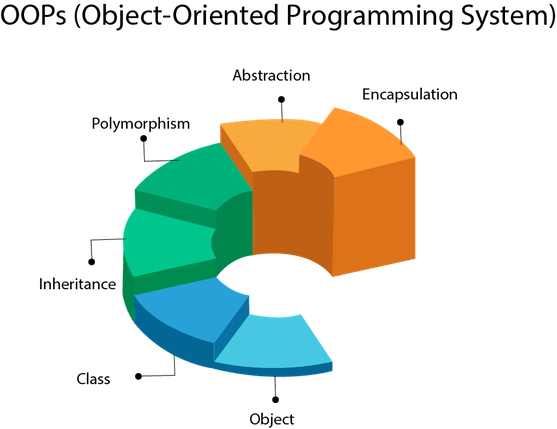
\includegraphics[width=7cm]{figure/literature/oop-programming.png}
  \caption[แผนผังองค์ประกอบของ OOPs]{แผนผังองค์ประกอบของการเขียนโปรแกรมแบบเชิงวัตถุ จาก~\cite{apollo22oop}}
  \label{fig:oop-concept}
\end{figure}
\thaijustify{
  องค์ประกอบของระบบโปรแกรมแบบเชิงวัตถุ (รูปที่~\ref{fig:oop-concept}) หรือ Object-Oriented Program System (หรือเรียกโดยย่อว่า OOPs) มีองค์ประกอบดังต่อไปนี้
}
\subsubsection{Objects และ Classes}
\thaijustify{
  วัตถุในเชิงของทฤษฎีนี้ คือขอบเขตข้อมูล (Data Field) ที่มีคุณสมบัติและพฤติกรรมเฉพาะ (Specific Properties and Behavior)~\cite{apollo22oop} วัตถุนั้นถมีความยืดหยุ่นเพื่อให้สอดคล้องกับวัตถุในโลกแห่งความเป็นจริง (Real-world Object) หรือสิ่งของเชิงนามธรรม (Abstract Entities)
}
\begin{figure}[H]
  \centering
  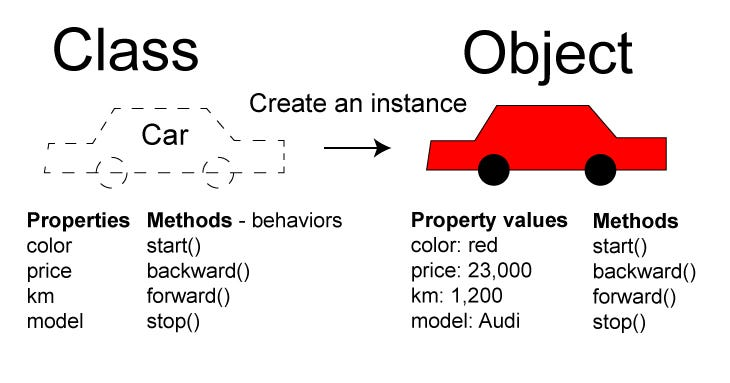
\includegraphics[width=6cm]{figure/literature/oop-class-object.jpg}
  \caption[แผนผังอธิบายความสัมพันธ์ระหว่างวัตถุและคลาส]{แผนผังอธิบายความสัมพันธ์ระหว่างวัตถุและคลาส จาก~\cite{moses22obj}}
  \label{fig:oop-class-obj}
\end{figure}
\thaijustify{
  สิ่งเหล่านี้เป็นวัตถุชั่วขณะ (หรือ Instances) สร้างขึ้นมาจากคลาส (Class) ซึ่งเปรียบเสมือนเป็นแม่พิมพ์หรือแบบแปลน (Blueprint) ที่สร้างขึ้นด้วยการใส่ค่าเริ่มต้นข้อมูลบางอย่างเข้าไปตอนเรียกการสร้าง (Instantiates) ตามรูปที่~\ref{fig:oop-class-obj}~\cite{apollo22oop}
}
\subsubsection{หลักการ Inheritance ของ Objects}
\thaijustify{
  การสืบทอดคุณลักษณะวัตถุ (หรือ Inheritance) เป็นกลไกของการสร้างวัตถุหรือคลาส โดยใช้ลักษณะจากวัตถุอื่น (Prototype-based Inheritance) หรือจากคลาส (Class-based Inheritance) การสร้างวัตถุหรือคลาสด้วยวิธีดังกล่าว จะคงไว้ซึ่งการใช้งาน ลักษณะและพฤติกรรมที่คล้ายคลึงกัน คลาสที่สร้างขึ้นมาจะถูกนิยามว่าคลาสย่อย (Subclass) และเรียกคลาสที่เป็นต้นแบบของคลาสย่อยว่าคลาสพื้นฐานหรือซุปเปอร์คลาส (Base Class or Superclass)~\cite{johnson88classobj}
}
\begin{figure}[H]
  \centering
  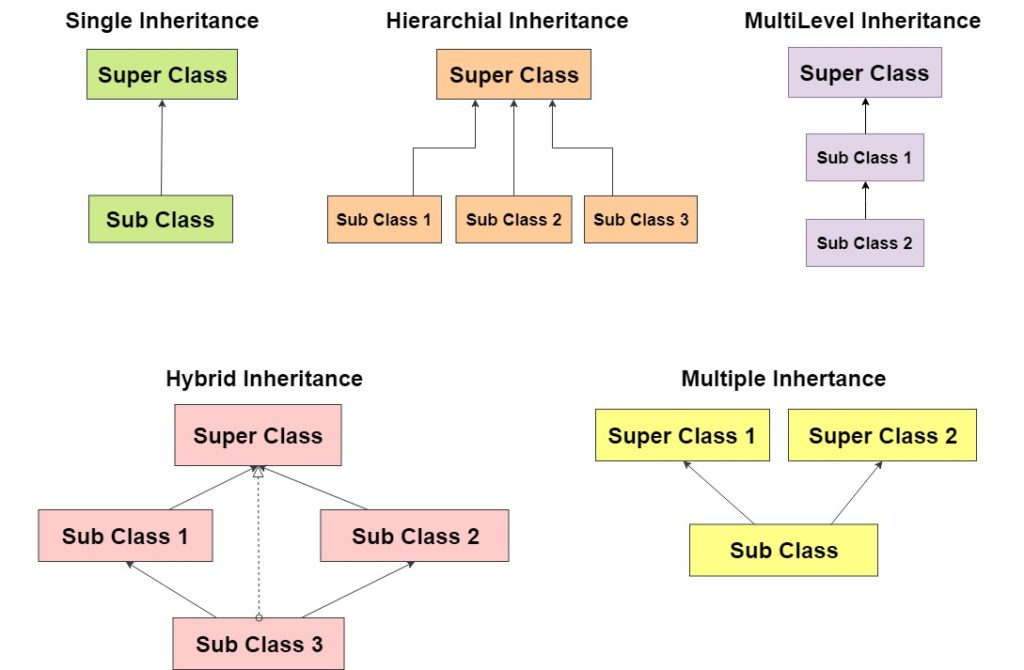
\includegraphics[width=9cm]{figure/literature/oop-inheritance.jpg}
  \caption[แผนผังอธิบายประเภทของการสร้างวัตถุด้วยการสืบทอดชนิดต่าง ๆ]{แผนผังอธิบายประเภทของการสร้างวัตถุด้วยการสืบทอด (Inheritance) ชนิดต่าง ๆ จาก~\cite{sakpal18inheritance}}
  \label{fig:oop-inheritance}
\end{figure}
\thaijustify{
  ใน~\cite{sakpal18inheritance} ได้แบ่งการสร้างวัตถุโดยการสืบทอดนั้นเป็น Single / Multiple / Hybrid ขึ้นกับจำนวนวัตถุที่วัตถุลูกสืบทอด หรือ Multilevel ถ้าหากคุณสมบัติของวัตถุถูกสืบทอดโดยวัตถุลูกมามากกว่าหนึ่งครั้งหรือหนึ่งชั้น หรือเรียกว่า Hierarchial ถ้าวัตถุชิ้นนั้นถูกสืบทอดโดยวัตถุลูกมากกว่าหนึ้งคลาส ตามรูปที่~\ref{fig:oop-inheritance} แต่ละภาษาโปรแกรมคอมพิวเตอร์มีการสนับสนุนการสร้างวัตถุด้วยการสืบทอดนั้นไม่เหมือนกัน ยกตัวอย่างเช่นภาษา Java นั้น ใช้ได้แค่ Single, Multilevel, และ Hierarchical Inheritance เท่านั้น, ภาษา C++ สามารถที่จะใช้ Multiple Inheritance ได้~\cite{stroustrup94inheritance} เป็นต้น
}
\subsubsection{หลักการ Polymorphism}
\thaijustify{
  จาก~\cite{javapolymorph} หลักการ Polymorphism เป็นการนำหลักการทางชีววิทยาที่กล่าวว่า "สิ่งมีชีวิตหรือสปีชีส์สามารถมีได้หลายรูปแบบหรือระยะต่าง ๆ" มาประยุกต์ ใช้งานในการเขียนโปรแกรมเชิงวัตถุ โดยถูกนำมาใช้เป็นหลักการจัดสร้างระบบประสานงานกับวัตถุอื่น (Object Interface) อันเดียวในคลาสหรือวัตถุใดๆ แต่ส่วนประสานดังกล่าวนั้น มีความพิเศษที่มันสามารถอนุญาตให้วัตถุหรือตัวตน (Entities) ประเภทอื่น ๆ มาเข้าใช้งาน
}
\thaijustify{
  คำว่า Polymorphism มาจากรากศัพท์ภาษาอังกฤษสองคำ; Poly แปลว่า มากมาย และ Morph แปลว่า รูปร่าง ดังนั้น เมื่อเราพูดถึงความหลากหลายในการเขียนโปรแกรม มันก็เหมือนกับการบอกว่าบางสิ่งบางอย่างสามารถมีได้หลายรูปแบบ ในการเขียนโปรแกรมเชิงวัตถุ (OOP) ความหลากหลายจะช่วยจัดการว่าส่วนต่างๆ ของโปรแกรมต้องพึ่งพาซึ่งกันและกันอย่างไร ช่วยให้การดำเนินการทำงานแตกต่างออกไปขึ้นอยู่กับข้อมูลที่กำลังทำงานอยู่~\cite{nzeruekenneth23polymorph}
}
\thaijustify{
  ลองนึกภาพคุณมีฟังก์ชันที่สามารถทำสิ่งต่าง ๆ ได้ตามสถานการณ์ ตัวอย่างเช่น วัตถุ "รูปร่าง" อาจมีฟังก์ชัน "วาด" เมื่อเรียกคำสั่ง "วาด" บนวงกลม มันจะวาดวงกลม เมื่อเรียกคำสั่ง "วาด" บนสี่เหลี่ยมจัตุรัส มันจะวาดรูปสี่เหลี่ยมจัตุรัส นี่คือการกระทำที่มีความหลากหลาย - ฟังก์ชันเดียวกันจะมีพฤติกรรมแตกต่างกันไปขึ้นอยู่กับวัตถุที่ใช้คำสั่งนั้นด้วย~\cite{ntu20polymorph}
}
\begin{figure}[H]
  \centering
  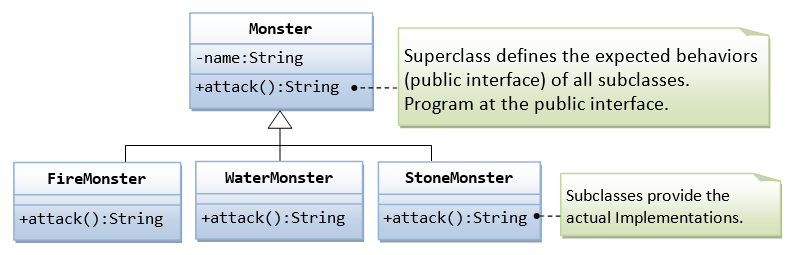
\includegraphics[width=10cm]{figure/literature/oop-polymorphism.png}
  \caption[แผนผังแสดงตัวอย่างของ Polymorphism ใน OOPs]{แผนผังแสดงตัวอย่างของ Polymorphism ใน OOPs จาก~\cite{ntu20polymorph}}
  \label{fig:oop-polymorph}
\end{figure}
\thaijustify{
  ใน~\cite{ntu20polymorph} ได้ให้รูปที่~\ref{fig:oop-polymorph} มาดูประกอบเป็นตัวอย่าง ถ้าในเกมของเรา เรามีมอนสเตอร์หลายประเภทที่สามารถโจมตีได้ เราจะออกแบบซูเปอร์คลาสที่เรียกว่า Monster และกำหนดวิธีการโจมตีในซูเปอร์คลาส (Superclass) จากนั้นคลาสย่อย (Subclass) ก็จะต้องนำกฎเกณฑ์ของซูเปอร์คลาสนำไปสร้างและปฏิบัติใหม่ (Implement) เป็นการโจมตีของมอนสเตอร์รูปแบบใหม่  แล้วในโปรแกรมหลัก หากเรียกใช้งานมอนสเตอร์ให้โจมตี มอนสเตอร์ก็จะโจมตีขึ้นกับประเภทของมอนสเตอร์นั้นที่กำลังโจมตี (FireMonster, WaterMonster หรือ StoneMonster)
}
\thaijustify{
  จากตัวอย่างดังกล่าวจะเห็นได้ว่า การทำ Polymorphism ใน OOPs ทำให้โปรแกรมเมอร์สามารถเขียนโปรแกรมที่อินเทอร์เฟซในการออกแบบระบบที่ซับซ้อน คลาสย่อยจะมีคุณลักษณะและการดำเนินการทั้งหมด เหมือนกับซูเปอร์คลาส (เนื่องจากคลาสย่อยสืบทอดคุณลักษณะและการดำเนินการทั้งหมดจากซูเปอร์คลาส) ซึ่งหมายความว่าวัตถุในคลาสย่อยนั้น สามารถจะทำอะไรก็ได้ที่ซูเปอร์คลาสสามารถทำได้ ด้วยเหตุนี้ เมื่อเราใช้อินสแตนซ์ (Instance) ของซูปเปอร์คลาส มันสามารถที่จะทดแทนคลาสย่อยได้ และทุกอย่างจะทำงานได้ตามปกติ (เรียกคุณสมบัตินี้ใน OOPs ว่า Substitutability)~\cite{ntu20polymorph}
}
\thaijustify{
  กล่าวสรุปก็คือ ความหลากหลายหมายความว่าวัตถุสามารถทำสิ่งต่าง ๆ ในสถานการณ์ที่แตกต่างกันได้ เช่นเดียวกับที่บุคคลสามารถเป็นสามี พ่อ หรือลูกชายได้ ขึ้นอยู่กับว่าพวกเขากำลังโต้ตอบด้วย วัตถุในการเขียนโปรแกรมสามารถมีบทบาทที่แตกต่างกัน ขึ้นอยู่กับบริบท~\cite{nzeruekenneth23polymorph}
}
\subsubsection{การทำ Abstraction}
\thaijustify{
  เป็นการคลาสที่กฎเกณฑ์ คุณสมบัติ และความสัมพันธ์ที่ถูกนิยามขึ้นโดยไม่ขึ้นกับวัตถุทางกายภาพโดยตรง คือการสร้างหรือมองคลาสและวัตถุให้ที่เป็นโมเดลหรือต้นแบบ (Prototype or Model) นามธรรม ให้สอดคล้องกับโลกของความเป็นจริง~\cite{saladpukabstract}
}
\thaijustify{
  ในการเขียนโปรแกรม Abstraction หมายถึงการแยกสิ่งที่ทำออกจากวิธีการทำ~\cite{liskov87abstaction} ลองนึกภาพคุณมีงานที่ต้องทำให้เสร็จ เช่น การอบเค้ก เราไม่จำเป็นต้องรู้ทุกรายละเอียดเกี่ยวกับวิธีการทำงานของเตาอบ เพียงแค่ต้องรู้วิธีใช้มันอบเค้ก ในทำนองเดียวกัน ในการเขียนโปรแกรม วิธีแรกในการสรุปสิ่งต่าง ๆ เรียกว่า "ขั้นตอน"
}
\thaijustify{
  ขั้นตอนก็เหมือนกับสูตรการอบเค้ก เป็นชุดคำสั่งที่ทำงานหรือฟังก์ชันเฉพาะ หากต้องการทำงานนั้นในโปรแกรม เพียงแค่เรียกใช้ขั้นตอนเช่นเดียวกับการทำตามสูตรในการอบเค้ก ไม่จำเป็นต้องกังวลเกี่ยวกับวิธีการเขียนขั้นตอนหรือสิ่งที่เกิดขึ้นภายในนั้น ตราบใดที่ขั้นตอนนี้ทำในสิ่งที่ควรจะทำอย่างถูกต้องและมีประสิทธิภาพ คุณก็สามารถใช้มันในโปรแกรมของคุณได้โดยไม่จำเป็นต้องเข้าใจรายละเอียดทั้งหมดเกี่ยวกับวิธีการทำงานของมัน การแยกระหว่างสิ่งที่ทำและวิธีการทำทำให้การเขียนโปรแกรมง่ายขึ้นและจัดการได้ง่ายขึ้น
}
\subsubsection{การทำ Encapsulation}
\thaijustify{
  Encapsulation เป็นเหมือนการรวมข้อมูลและฟังก์ชันเข้าด้วยกัน จากงานศึกษาค้นคว้าของ \textit{Nzerue-Kenneth et al.}~\cite{nzeruekenneth23polymorph} เหมือนกับการใส่ไว้ในแคปซูลป้องกัน แนวคิดหลักคือการซ่อนความซับซ้อนของ Objects จากโปรแกรมและผู้ใช้ ทำให้ใช้งานได้ง่ายขึ้น มันคือทั้งหมดที่เกี่ยวกับการซ่อนการทำงานภายในของโค้ดไว้ ดังนั้นจึงไม่ต้องกังวลเกี่ยวกับวิธีการทำงาน แค่ใช้งานอย่างเดียวเท่านั้น
}
\begin{figure}[H]
  \centering
  \subfloat[การเปรียบเทียบการทำ Encapsulation กับยาแคปซูล~\cite{raut22encapsule}]{
    \fbox{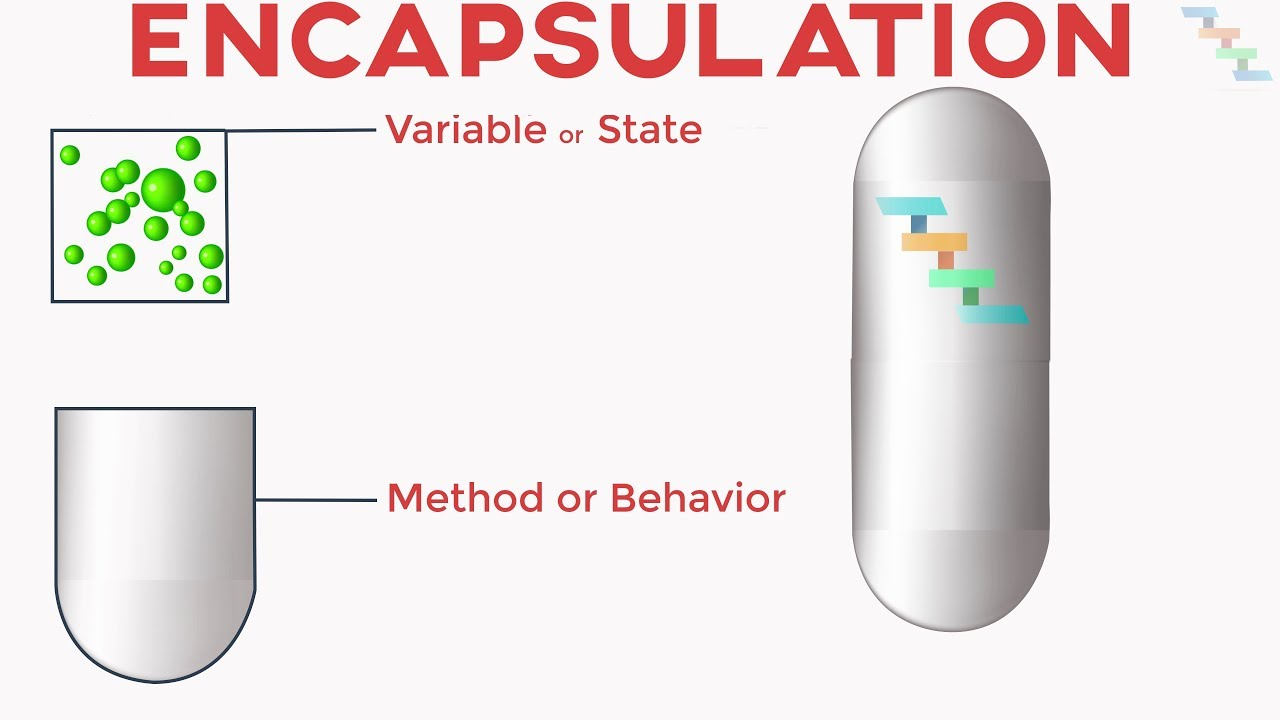
\includegraphics[width=6cm]{figure/literature/oop-encapsulation.png}}
    \label{fig:oop-encapsulation-capsule}
  }
  \subfloat[การทำ Encapsulation เพื่อปกปิดคุณสมบัติของคลาส~\cite{nishad22encapsulation}]{
    \fbox{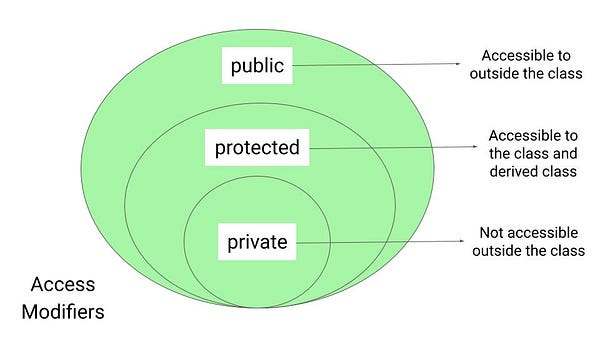
\includegraphics[width=6cm]{figure/literature/oop-encapsulation-detail.jpg}}
    \label{fig:oop-encapsulation-details}
  }
  \caption[แผนผังอธิบายการทำ Encapsulation]{แผนผังอธิบายการทำ Encapsulation}
  \label{fig:oop-encapsulation}
\end{figure}
\thaijustify{
  จากบทความของ \textit{Raut A.}~\cite{raut22encapsule} ได้เปรียบเทียบหลักการนี้กับแคปซูลที่ปกป้องยาที่อยู่ภายใน ตามในรูปที่~\ref{fig:oop-encapsulation-capsule} การห่อหุ้มของแคปซูลจะปกป้องข้อมูลและฟังก์ชันในโปรแกรม มันเชื่อมโยงโค้ดและข้อมูลที่มันทำงานด้วย สร้างเกราะป้องกันล้อมรอบพวกมัน ด้วยการห่อหุ้ม คุณสามารถจำกัดการเข้าถึงบางส่วนของออบเจ็กต์ โดยให้เฉพาะส่วนอื่น ๆ ของโปรแกรมเข้าถึงสิ่งที่พวกเขาต้องการเท่านั้น เหมือนกับมีตู้จำหน่ายสินค้าอัตโนมัติ คุณไม่สามารถเข้าไปซื้อขนมข้างในได้เว้นแต่คุณจะใช้ปุ่มของเครื่อง ในทำนองเดียวกัน ในการห่อหุ้ม ตัวแปรและฟังก์ชันของวัตถุจะถูกซ่อนไว้และสามารถเข้าถึงได้ผ่านวิธีการเฉพาะภายในคลาสของวัตถุนั้นเท่านั้น
}
\thaijustify{
  ดังนั้น การทำ Encapsulation คือทั้งหมดที่เกี่ยวกับการเก็บรักษาสิ่งของต่างๆ ให้ปลอดภัยและซ่อนไว้ตามรูปที่~\ref{fig:oop-encapsulation-details} เช่นเดียวกับยาในแคปซูลหรือของว่างในตู้จำหน่ายสินค้าอัตโนมัติ ช่วยให้โปรแกรมใช้งานและเข้าใจได้ง่ายขึ้นโดยปกป้องการทำงานภายในของโปรแกรมเหล่านั้น~\cite{nishad22encapsulation}
}
\thaijustify{
  จากที่กล่าวมา แม้ว่าจะฟังเหมือนว่าทฤษฎีหรือหลักการเขียนโปรแกรมเชิงวัตถุ จะสามารถทำให้การเขียนโปรแกรมและการสร้างซอฟต์แวร์ที่วับซ้อนดูง่ายขึ้น หลักการดังกล่าวก็มีข้อเสียเช่นกัน ข้อเสียเปรียบประการหนึ่งคือ ความง่ายดายต่อการถูกนำเอาไปแก้ไขปัญหาที่ง่าย (Over-engineer) นักพัฒนาอาจสร้างนามธรรม (Abstraction) ที่ไม่จำเป็นหรือลำดับชั้นที่ซับซ้อนซึ่งทำให้ Code base ยากต่อการเข้าใจและบำรุงรักษา โปรแกรมที่เขียนกลายเป็นของที่เข้าใจยากกว่าปัญหาที่ตนกำลังจะแก้~\cite{thomas99pragmatic} นอกจากนี้ การจัดการความสัมพันธ์ระหว่างคลาสและอ็อบเจ็กต์สามารถนำไปสู่การเชื่อมต่อที่แน่นแฟ้น ทำให้การแก้ไขหรือขยายโค้ดเป็นเรื่องที่ท้าทาย เพราะการเปลี่ยนแปลงโค้ด ณ จุดใดจัดหนึ่ง นั้นมีผลกระทบต่อส่วนอื่น ๆ ของระบบ~\cite{fowler13oop}
}
\thaijustify{
  กลุ่มคณะผู้จัดทำได้มีประสบการณ์ในการเขียนโปรแกรมหรือซอฟต์แวร์ที่มีรากฐานของแนวคิดงมาจากแนวคิดหรือทฤษฎีเชิงวัตถุเป็นอย่างดี ยกกรณีตัวอย่างการเขียนหน้าเว็บที่ซับซ้อน หากมองมีลักษณะการเขียนในเชิงกึ่งวัตถุ ด้วยการมองชิ้นส่วนองค์ประกอบหรือส่วนประกอบของส่วนประสานงานหน้าเว็บไซต์ (Website UI Component) ตัวอย่างเช่น พวกปุ่มหรือช่องกรอกข้อมูลในฟอร์ม เป็นวัตถุชิ้นหนึ่ง ที่มีฟังก์ชันและค่าข้อมูลในตัว การมองเช่นนี้จะทำให้หน้าเว็บที่ซับซ้อนนั้นเข้าใจง่ายยิ่งขึ้น สามารถที่จะพัฒนาชิ้นส่วนและองค์ประกอบของหน้าเว็บได้อย่างง่ายได้ ทำให้ในขั้นตอนการพัฒนาซอฟต์แวร์ดำเนินไปได้สะดวกในระดับหนึ่ง เนื่องจากถ้าอิงจากหลักการดังกล่าว หากทำการเปลี่ยนแปลงลักษณะหรือโค้ดของวัตถุใดวัตถุหนึ่ง จะไม่กระทบกระเทือนวัตถุอื่นมากนัก เนื่องจากแต่ละวัตถุนั้นมีบทบาทหน้าที่แยกออกจากกันอย่างชัดเจน (โดยหลักการ SoC ที่ใช้ควบคู่กับ OOPs ที่จะพูดถึงและบรรยายในหัวข้อถัดไป)
}
\subsection{หลักการ Separation of Concern}
\thaijustify{
  หลักการ Separation of Concern (หรือ SoC โดยย่อ) หรืออาจเรียกว่าหลักการออกแบบซอฟต์แวร์ด้วยการแบ่งแยกข้อกังวล เป็นแนวคิดการออกแบบหนึ่งในสาขาวิชาวิศวกรรมซอฟต์แวร์ โดยเน้นถึงความจำเป็นในการแบ่งระบบที่ซับซ้อนออกเป็นส่วนที่แตกต่างกันและจัดการได้ ซึ่งแต่ละส่วนจะกล่าวถึงลักษณะเฉพาะของฟังก์ชันการทำงาน (Function) หรือภาระหน้าที่ (Concern หรือ Responsibility)~\cite{nattawat20pgs}
}
\begin{figure}[H]
  \centering
  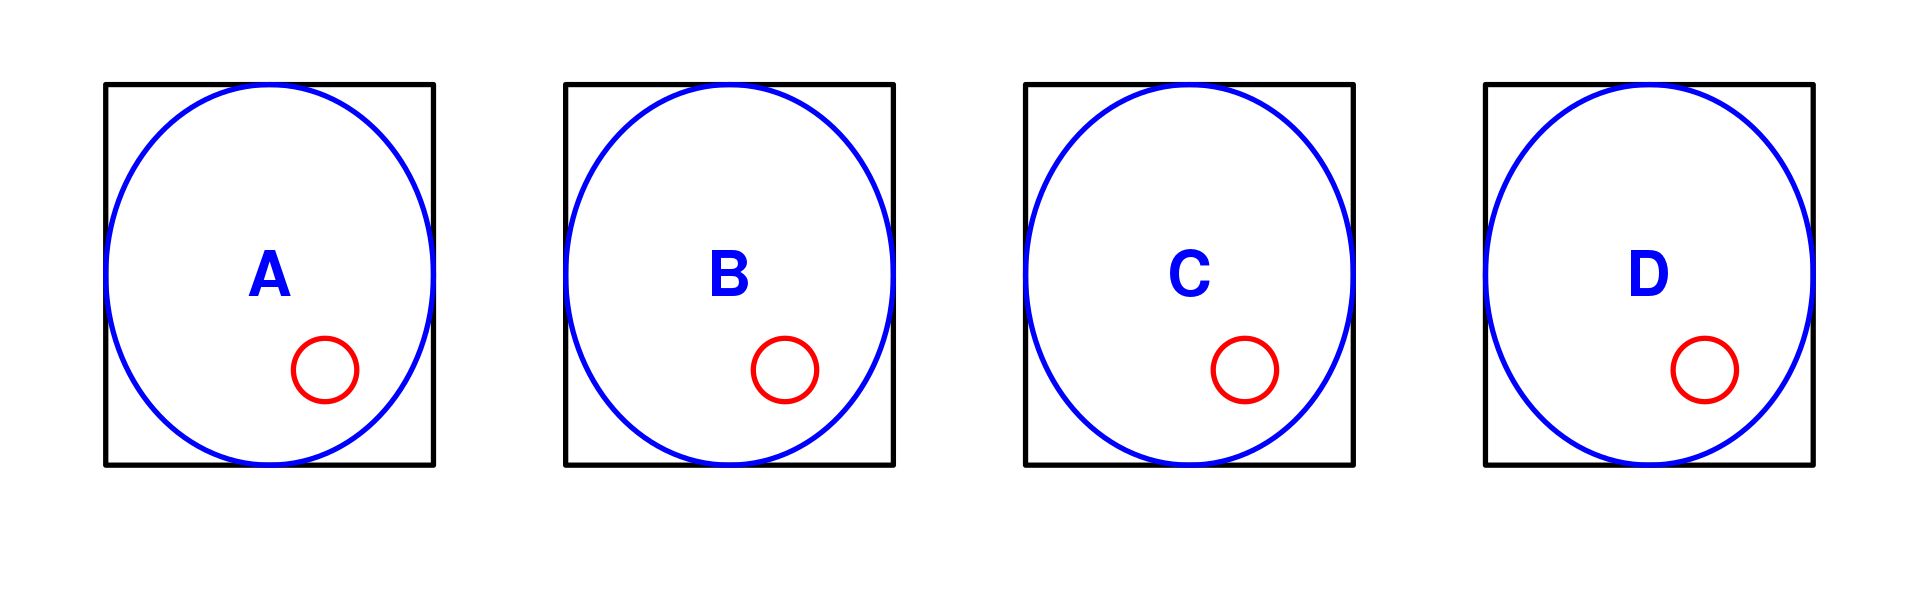
\includegraphics[width=6cm]{figure/literature/soc.png}
  \caption[แผนผังแสดงหลักการ Separation of Concern]{แผนผังแสดงหลักการ Separation of Concern จาก~\cite{wikipedia04soc}}
  \label{fig:soc-general}
\end{figure}
\thaijustify{
  หลักการนี้มีบทบาทสำคัญในการปรับปรุงคุณภาพซอฟต์แวร์ การบำรุงรักษา และความสามารถในการขยาย~\cite{dijkstra82} ในขอบเขตของสถาปัตยกรรมซอฟต์แวร์ การแยกข้อกังวลมักจะเกี่ยวข้องกับการแบ่งระบบออกเป็นโมดูล (Modules) หรือส่วนประกอบ (Components) โดยแต่ละส่วนจะเกี่ยวข้องกับลักษณะเฉพาะของแอปพลิเคชันเช่น ส่วนติดต่อผู้ใช้ (User Interface) การจัดเก็บข้อมูล (Data Collections) หรือตรรกะทางธุรกิจ (Business Rules/Logic) แนวทางนี้จะลดการพึ่งพาซึ่งกันและกันระหว่างส่วนต่างๆ ของซอฟต์แวร์ ทำให้ง่ายต่อการพัฒนา แก้ไข และดีบักซอฟต์แวร์~\cite{wikipedia04soc} เนื่องจากการเปลี่ยนแปลงในด้านหนึ่งมีโอกาสน้อยที่จะส่งผลกระทบต่อส่วนอื่น ๆ มันส่งเสริมฐานรหัสที่มีการจัดระเบียบและเข้าใจได้มากขึ้น ซึ่งอำนวยความสะดวกในการทำงานร่วมกันระหว่างนักพัฒนา
}
\thaijustify{
  หลักการนี้ถูกนำไปใช้ในการเขียนโปรแกรมแบบเชิงวัตถุ หรือ Object-Oriented Programming (การเขียนโปรแกรมด้วยการมองตัวไฟล์คำสั่งเป็นวัตถุหนึ่ง ๆ) ซึ่งเป็นการเขียนโปรแกรมหรือหลักการสร้างซอฟต์แวร์ที่นิยมเป็นอย่างมาก โดยเฉพาะอย่างยิ่งในซอฟต์แวร์ที่ซับซ้อน เห็นได้จากความเห็นของ \textit{Meyer}~\cite{meyer2000} ที่กล่าวว่า "หลักการดังกล่าวเป็นการสร้างซอฟต์แวร์ที่เป็นคุณภาพและมั่นคง มันทำให้รักษาความเข้าใจ, ความถูกต้องและประสิทธิภาพของแต่ละส่วนในระบบ" กล่าวคือการพัฒนาซอฟต์แวร์ใช้หลักการการแยกปัญหาและหน้าที่ของแต่ละองค์ประกอบที่ชัดเจน นำไปสู่การพัฒนาระบบซอฟต์แวร์ที่มีประสิทธิภาพและเครื่องมือที่มีคุณภาพสูง
}
\thaijustify{
  ในโครงงานปริญญานิพนธ์ของ \textit{Jamlongrad et al.}~\cite{nattawat20pgs} ที่คณะผู้จัดทำใช้อ้างอิงเป็นหลักก็ได้มีการนำหลักการ Separation of Concern มาใช้ร่วมเช่นกัน เพราะเนื่องจากระบบของโครงการดังกล่าวนั้น เขียนขึ้นมาด้วยหลักการเขียนโปรแกรมเชิงวัตถุ หรือ Object-Oriented Programming เช่นเดียวกับกลุ่มคณะผู้จัดทำ
}
\subsection{หลักการ Version Control}
\thaijustify{
  การทำ Version Control คือการจัดการซอร์สโค้ด (หรือ Source code) ซึ่งเป็นกระบวนการที่สำคัญในการพัฒนาซอฟต์แวร์ จำเป็นต้องมีการติดตามและการจัดการการเปลี่ยนแปลงใน Code base ของโครงการ~\cite{nattawat20pgs, rawat22versionctl}
}
\thaijustify{
  โดยเครื่องมือดังกล่าวช่วยให้นักพัฒนาซอฟต์แวร์หลายคน สามารถทำงานร่วมกันในโครงการซอฟต์แวร์โดยจัดให้มีวิธีที่เป็นระบบในการติดตามการเปลี่ยนแปลงที่เกิดขึ้นกับซอร์สโค้ด แนวทางปฏิบัตินี้ช่วยเพิ่มองค์กร ความโปร่งใส และความเสถียรของโครงการซอฟต์แวร์ ช่วยให้นักพัฒนาสามารถดูและเข้าใจประวัติการเปลี่ยนแปลง แยกและแก้ไขปัญหา และจัดการงานที่เกิดขึ้นพร้อมกันได้อย่างมีประสิทธิภาพ~\cite{rawat22versionctl} หนึ่งในเครื่องมือ Version Control ที่นักพัฒนาหลายคนรู้จักและนิยมใช้ก็คือ Git ซึ่งปรากฎให้ใช้ในเว็บไซต์หรือเว็บแอปพลิเคชัน ที่ชื่อว่า GitHub กับ GitLab~\cite{chacon14}
}
\begin{figure}[H]
  \centering
  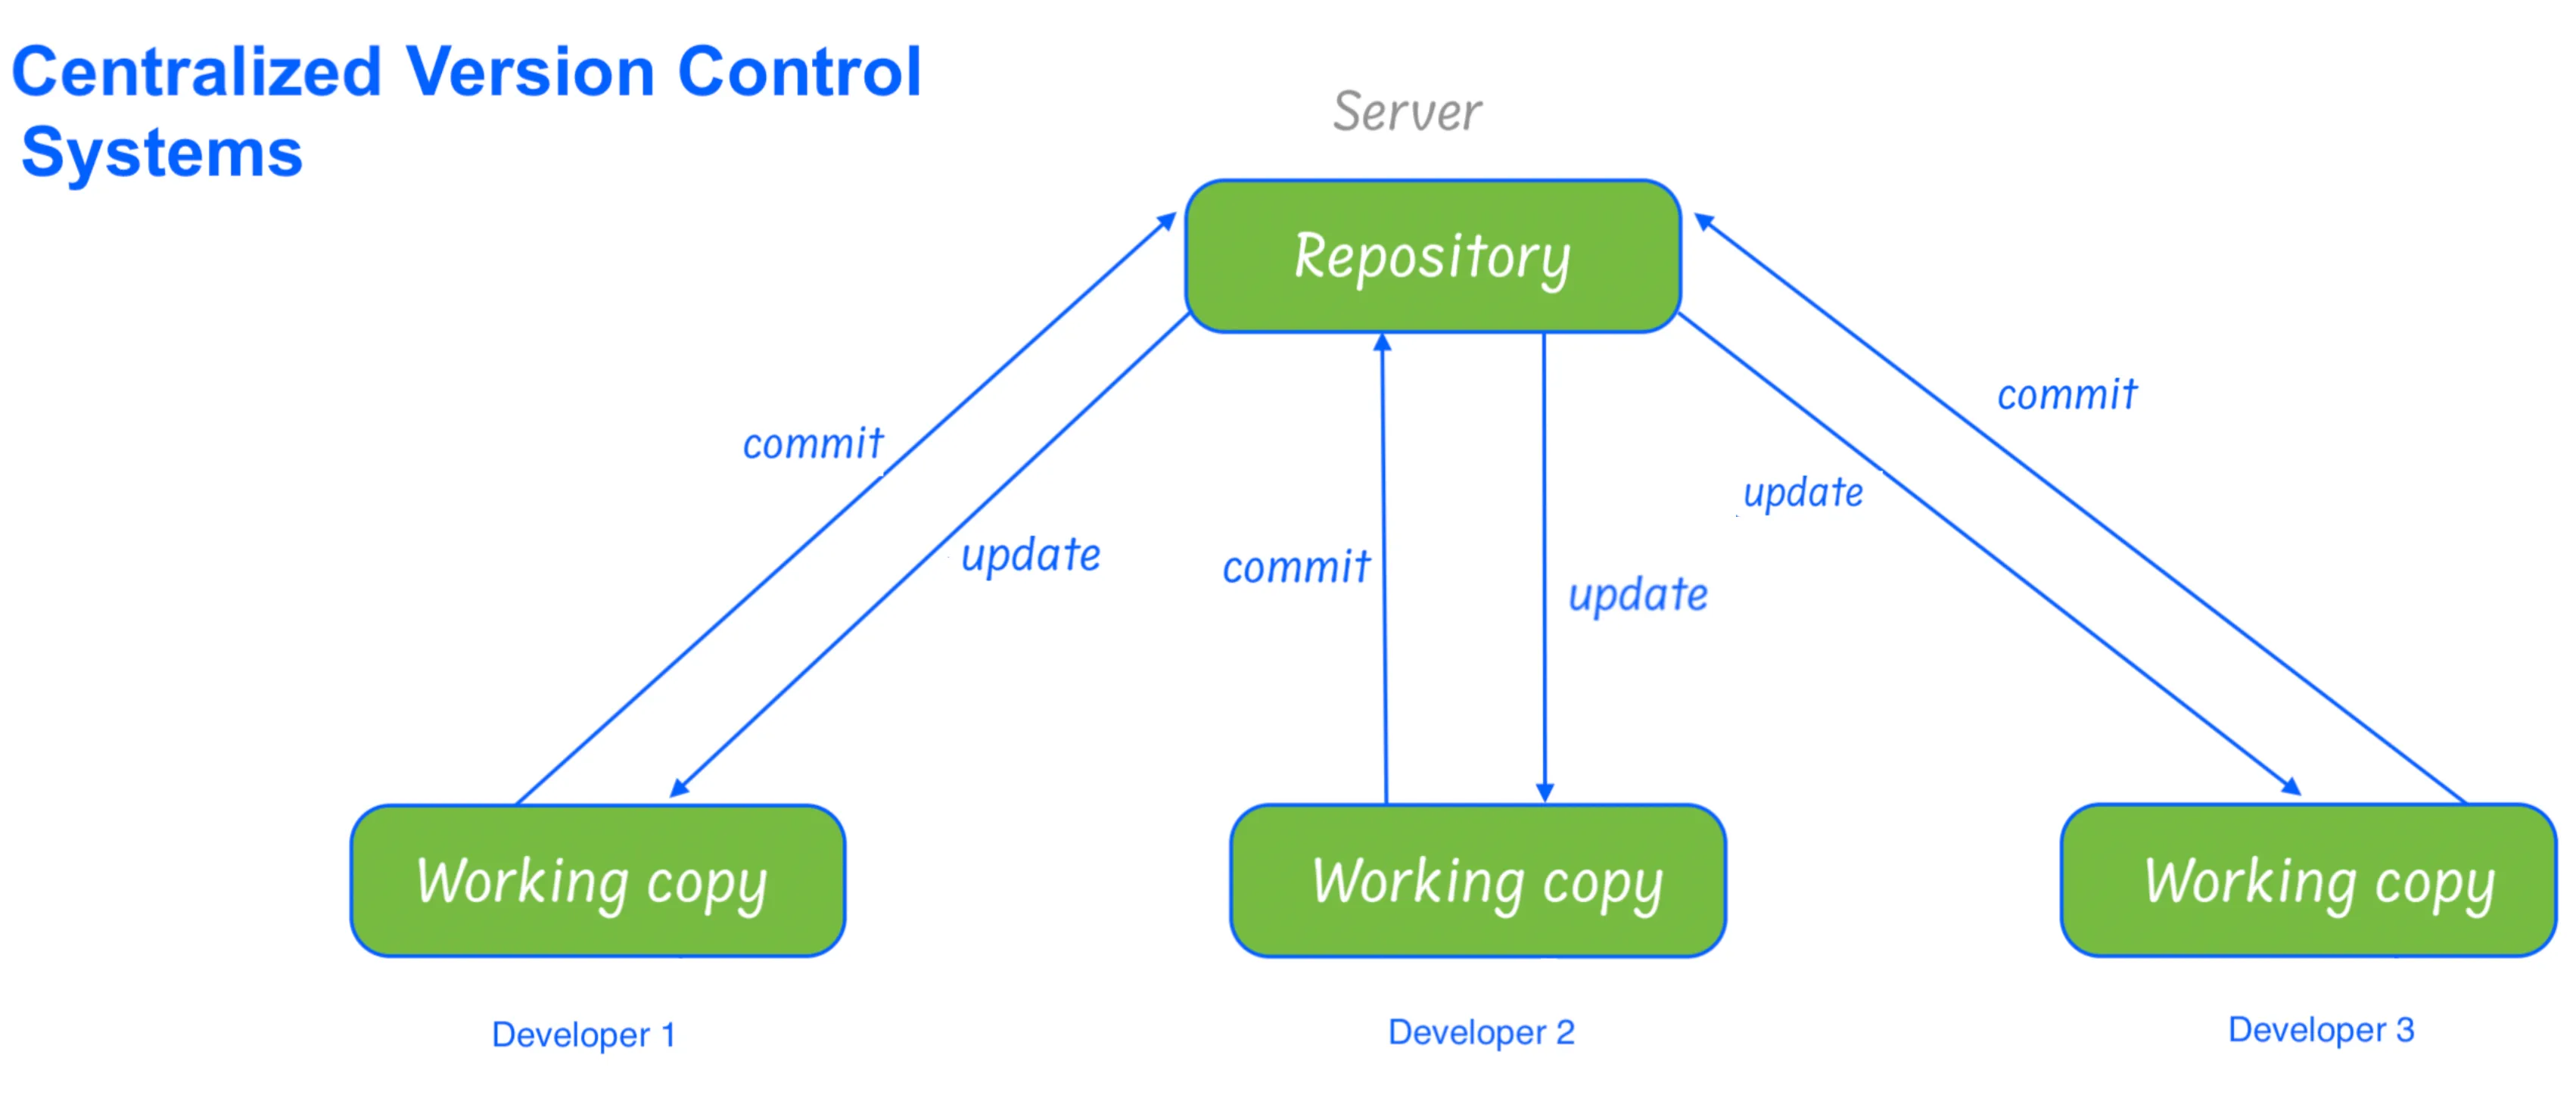
\includegraphics[width=9cm]{figure/literature/version-control.png}
  \caption[แผนผังอธิบายการทำงานของระบบ Version control]{แผนผังอธิบายการทำงานของระบบ Version control จาก~\cite{rawat22versionctl}}
  \label{fig:version-control}
\end{figure}
\thaijustify{
  โดย Git เสนอแนวทางแบบกระจายและอเนกประสงค์ ซึ่งสนับสนุนการแยกสาขา (Branch) และการผสานรวม (Merge) ช่วยให้นักพัฒนาสามารถทำงานกับคุณสมบัติต่างๆ ได้พร้อมๆ กัน และรวมงานของพวกเขาได้อย่างราบรื่นในภายหลัง (ตามรูปที่~\ref{fig:version-control}) หลักการนี้จำเป็นสำหรับการรับประกันความสมบูรณ์ของโครงการซอฟต์แวร์โดยจัดให้มีกลไกในการเปลี่ยนกลับเป็น version ก่อนหน้า กู้คืนจากข้อผิดพลาด (Rollbacks) และรักษาประวัติการเปลี่ยนแปลงโค้ดที่เชื่อถือได้ ซึ่งทั้งหมดนี้มีส่วน ช่วยในการจัดการโครงการ และทำให้แน่ใจว่าการทำงานจะดำเนินไปอย่างราบรื่น
}
\thaijustify{
  ในการพัฒนาซอฟต์แวร์หลายงาน หลายบริษัทและองค์กร รวมไปถึงโครงงานปริญญานิพนธ์ของ~\textit{๋Jamlongrad et al.}~\cite{nattawat20pgs} และ \textit{CodeForces}~\cite{codeforces} ล้วนแต่ใช้ระบบ Version Controlเป็นซอฟต์แวร์ตรวจโปรแกรมภาษาซีเหมือนกับโครงการของคณะผู้จัดทำ นั้น ก็ได้มีการนำหลักการ และเครื่องมือ Version Control มาใช้ร่วมเเละควบคู่กับการบริหารซอฟต์เเวร์ในโครงงาน เนื่องจากพัฒนาซอฟต์แวร์ต้องทำงานกันเป็นกลุ่ม การใช้ Version Control เข้ามาช่วยในการจัดการบริหารการเปลี่ยนแปลงของซอร์สโค้ด ช่วยให้การทำงานสะดวกยิ่งขึ้น ไม่เสียเวลากับการจัดการไฟล์ซอร์สโค้ดเองด้วยมือ แล้วสามารถเอาเวลาไปมุ่งเน้นกับการการพัฒนาโปรแกรม
}
\subsection{หลักการ Continuous Integration และ Continuous Delivery}
\thaijustify{
  หลักการ Continuous Integration (CI) และ Continuous Delivery (CD) นิยมเรียกรวมกันโดยย่อว่าหลักการ CI/CD เป็นหลักการพื้นฐานในการพัฒนาซอฟต์แวร์สมัยใหม่ที่เน้นไปที่การพัฒนาซอฟต์แวร์ควบคู่กับการส่งมอบซอฟต์แวร์ไปสู่การผลิต (Production) โดยอัตโนมัติ เพื่อเสริมสร้างการทำงานซอฟต์แวร์ที่มีประสิทธิภาพและรวดเร็วให้ได้มากที่สุด
}
\thaijustify{
  โดยเกี่ยวข้องกับการรวมการเปลี่ยนแปลงโค้ดทั้งหมดเข้ากับไปในพื้นที่เก็บข้อมูลที่ใช้ร่วมกัน Shared repository สม่ำเสมอ จากนั้นก็จะนำไปถูกสร้างขึ้นเป็นซอฟต์แวร์พร้อมใช้งาน หรือ Production build จากนั้นก็นำไปเข้าทดสอบหาข้อผิดพลาด (Test) ถ้าหากทดสอบผ่านก็จะนำเอาซอฟต์แวร์ดังกล่าวมาเปิดใช้ (Deploy) กับสภาพแวดล้อมต่างๆ (Environment) โดยอัตโนมัติ~\cite{fowlerCI}
}
\thaijustify{
  แนวทางปฏิบัติหรือกระบวนการดังกล่าว จะช่วยเร่งกระบวนการทำงานและกระบวนการพัฒนาซอฟต์แวร์ ลดปัญหาในขั้นตอนการนำซอฟต์แวร์ไปจัดวางและเปิดใช้งาน และทำให้มั่นใจได้ว่าซอฟต์แวร์จะอยู่ในสภาพที่พร้อมใช้งานอยู่เสมอ โดยหลักการดังกล่าวจะนิยมไปใช้ควบคู่กับการ Version Control โดยเฉพาะบน Git
}
\thaijustify{
  ตัวอย่างการใช้ ก็มีให้เห็นได้อย่างชัดเจนในโครงงานของ~\textit{๋Jamlongrad et al.}~\cite{nattawat20pgs} ในรายงานก็มีการใช้เครื่องมือที่ชื่อ Argo กับ Drone ในการทำ CI/CD โดยเครื่องมือดังกล่าวจะนำไฟล์งานซอฟต์แวร์ที่ได้เขียนไว้ (Development build) ไปสร้างเป็นซอฟต์แวร์พร้อมใช้งาน (Production Build) จากนั้นก็นำไปสร้างและจัดวาง (Deploy) เปิดใช้งานในเซิร์ฟเวอร์ปลายทาง
}
\subsection{ลักษณะการออกแบบโปรแกรมรูปแบบ Dependencies Injection}
\thaijustify{
  Dependencies Injection หรือนิยมย่อกันว่า DI เป็นรูปแบบการออกแบบ (Design Pattern) ในที่ใช้กันทั่วไปในการพัฒนาซอฟต์แวร์เชิงวัตถุ เพื่อจัดการการขึ้นต่อกัน (Dependencies) ของคลาสหรือโมดูลโดยการนิยามหรือสร้างไว้ข้างนอก (Provided Externally) แทนที่จะสร้างข้างใน ใน DI การขึ้นต่อกันจะถูก "ฉีด" (หรือ Inject) เข้าไปในคลาสหรือโมดูลจากภายนอก กล่าวสั้น ๆ ง่าย ๆ โดยใช้คำนิยามของ \textit{Shore J.} ที่กล่าวว่า "Dependencies Injection หมายถึงการให้ตัวแปร Instance แก่วัตถุ"~\cite{shore06} ก็คือการใช่รูปแบบการออกแบบนี้ ก็แค่ให้ หรือฉีดข้อมูล ตัวแปร หรือฟังก์ชันเข้าไปในวัตถุที่ต้องการเองด้วยมือ ด้วยหนึ่งในวิธีการ Inject สามประเภทได้แก่การฉีดคอนสตรัคเตอร์ (Constructor) ตัวตั้งค่า (Setter) หรืออินเตอร์เฟส (Interface)
}
% TODO: Add example of deps injections
% Some sources
% - https://www.codeproject.com/Articles/615139/An-Absolute-Beginners-Tutorial-on-Dependency-Inver
% - https://deviq.com/practices/dependency-injection
\thaijustify{
  วิธีการดังกล่าว ส่งเสริมให้การเชื่อมต่อที่หลวม (Loosely coupled) ระหว่างวัตถุ หรือส่วนประกอบต่าง ๆ ของโปรแกรม~\cite{fowlerDI} ซึ่งการที่วัตถุมีการเชื่อมต่อที่หละหลวมก็ทำให้เกิดข้อดีเช่นกัน อย่างเช่นทำให้โปรแกรมนั้นสามารแยกส่วนประกอบออกมาทดสอบได้ (Testability) สามารถที่จะนำ Unit test มาใช้ทดสอบซอฟต์แวร์หรือโปรแกรมดังกล่าวได้ ถ้าหากองค์ประกอบสามารถที่แยกส่วนประกอบออกได้อย่างชัดเจน อีกข้อดีหนึ่งก็คือซอฟต์แวร์หรือโปรแกรมนั้นจะสามารถบำรุงรักษาได้ง่าย (Maintainability) เพราะการเปลี่ยนแปลงโค้ดที่จุดใดจุดหนึ่งในซอฟต์แวร์จะไม่กระทบให้ส่วนอื่นเปลี่ยนแปลงไปมาก~\cite{freeman09}
}
\thaijustify{
  ข้อดีอีกประการหนึ่งที่คณะผู้จัดทำให้ความสนใจเป็นพิเศษและอยากมาทดลองใช้ในโครงงาน เป็นข้อดีที่ผู้ใช้ที่มีนามสมมุติว่า \textit{Tiwari G.} (นามแฝงว่า \textit{gtiwari333}) ได้บอกใน \textit{Stack Overflow}~\cite{tiwaristackdi} คือการที่ Dependencies injection นั้นยอมให้ผู้พัฒนาฉีด Dependency แบบปลอม ๆ (Mock dependencies) เข้าไปในคลาสได้ แทนที่จะใช้ Dependencies ของจริง ด้วยวิธีการนี้ซอฟต์แวร์หรือโปรแกรมที่อยู่ในขั้นของการพัฒนา (Development phase) จะสามารถที่จะทดสอบ Dependency ส่วนที่ผู้พัฒนากำลังเขียนอยู่ได้ โดยไม่ต้องไปเปลี่ยนแปลงโค้ดส่วนอื่นที่ไม่ได้อยู่ในขอบเขตการทดสอบ โดยรวมทำให้การทำงานง่ายขึ้น
}
\thaijustify{
  อย่างไรก็ตาม การใช้ Dependencies Injection ก็ยังมีข้อเสียที่อาจเกิดขึ้นเช่นกัน ตามที่ \textit{Toan T.} ได้ให้ความเห็นใน \textit{Stack Overflow}~\cite{toanstackdi} เมื่อใช้ Dependency Insert ข้อกังวลหลักคือความซับซ้อนที่เพิ่มขึ้น ซึ่งจะทำให้ทรัพยากรที่โปรแกรมหรือซอฟต์แวร์ดังกล่าวใช้เพิ่มมากขึ้น แม้ว่าเฟรมเวิร์ก DI จะทำให้กระบวนการจัดการการขึ้นต่อกันเป็นไปโดยอัตโนมัติ แต่ก็สามารถทำให้โค้ดของโปรแกรมซับซ้อนขึ้นเช่นกัน ทำให้อ่านเข้าใจยากขึ้น
}
\section{โครงงาน งานวิจัยหรือผลิตภัณฑ์ที่เกี่ยวข้อง}
เนื่องจากทางกลุ่มคณะผู้จัดทำพัฒนาซอฟต์แวร์ประเภทและรูปแบบนี้เป็นครั้งแรก ทางกลุ่มจึงต้องไปศึกษาหาซอฟต์แวร์อื่น ๆ ที่ทำงานและเปิดให้บริการด้านการตรวจงานเขียนภาษาโปรแกรมเช่นเดียวกับโครงการของคุณะผู้จัดทำ มาใช้อ้างอิงและวิเคราะห์หาข้อดีและข้อเสีย เพื่อนำมาประยุกต์ใช้ในขั้นตอนการสร้างซอฟต์แวร์โครงการนี้
\subsection{IPST Program Grader}
\thaijustify{
  \href{https://programming.in.th}{IPST Program Grader} เป็นเว็บไซต์ แอปพลิเคชันที่สร้างขึ้นโดย\textit{สถาบันส่งเสริมการสอนวิทยาศาสตร์และเทคโนโลยี (สสวท.)}~\cite{ipstGrader} ถูกนำมาปรับปรุงใหม่โดยกลุ่มนักเรียนค่ายโอลิมปิกวิชาการคอมพิวเตอร์ในช่วงล่าสุดนี้ เว็บไซต์ดังกล่าวถูกสร้างขึ้นมาเพื่อให้ผู้ใช้สามารถเข้ามาฝึกฝนทักษะการเขียนโปรแกรม เรียนรู้การเขียนโปรแกรม เรียนรู้เกี่ยวกับโครงสร้างข้อมูล และฝึกเขียนอัลกอริทึมที่มีประสิทธิภาพ
}
\begin{figure}[H]
  \centering
  \subfloat[หน้าหลักเว็บไซต์ ณ วันที่ 10 ธันวาคม 2562~\cite{ipstGrader}]{
    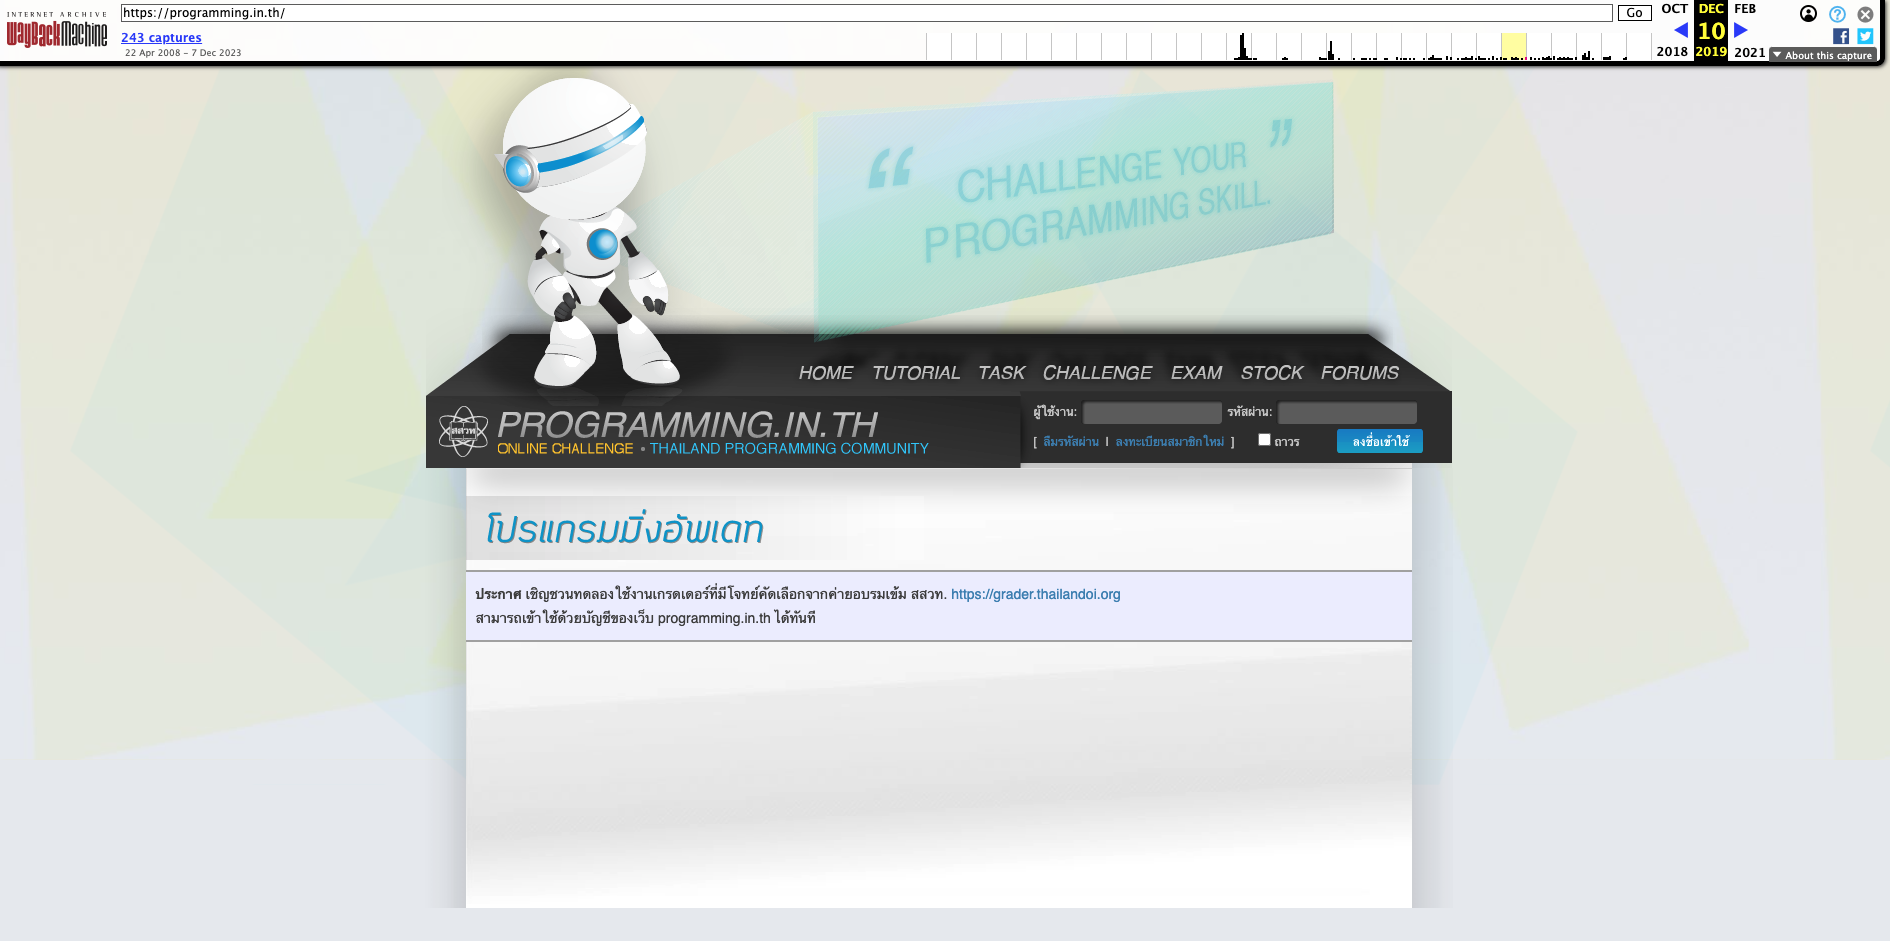
\includegraphics[width=7cm]{figure/literature/old-ipst.png}
    \label{fig:ipst-page-old}
  }
  \subfloat[หน้าหลักเว็บไซต์ ณ ปัจจุบัน]{
    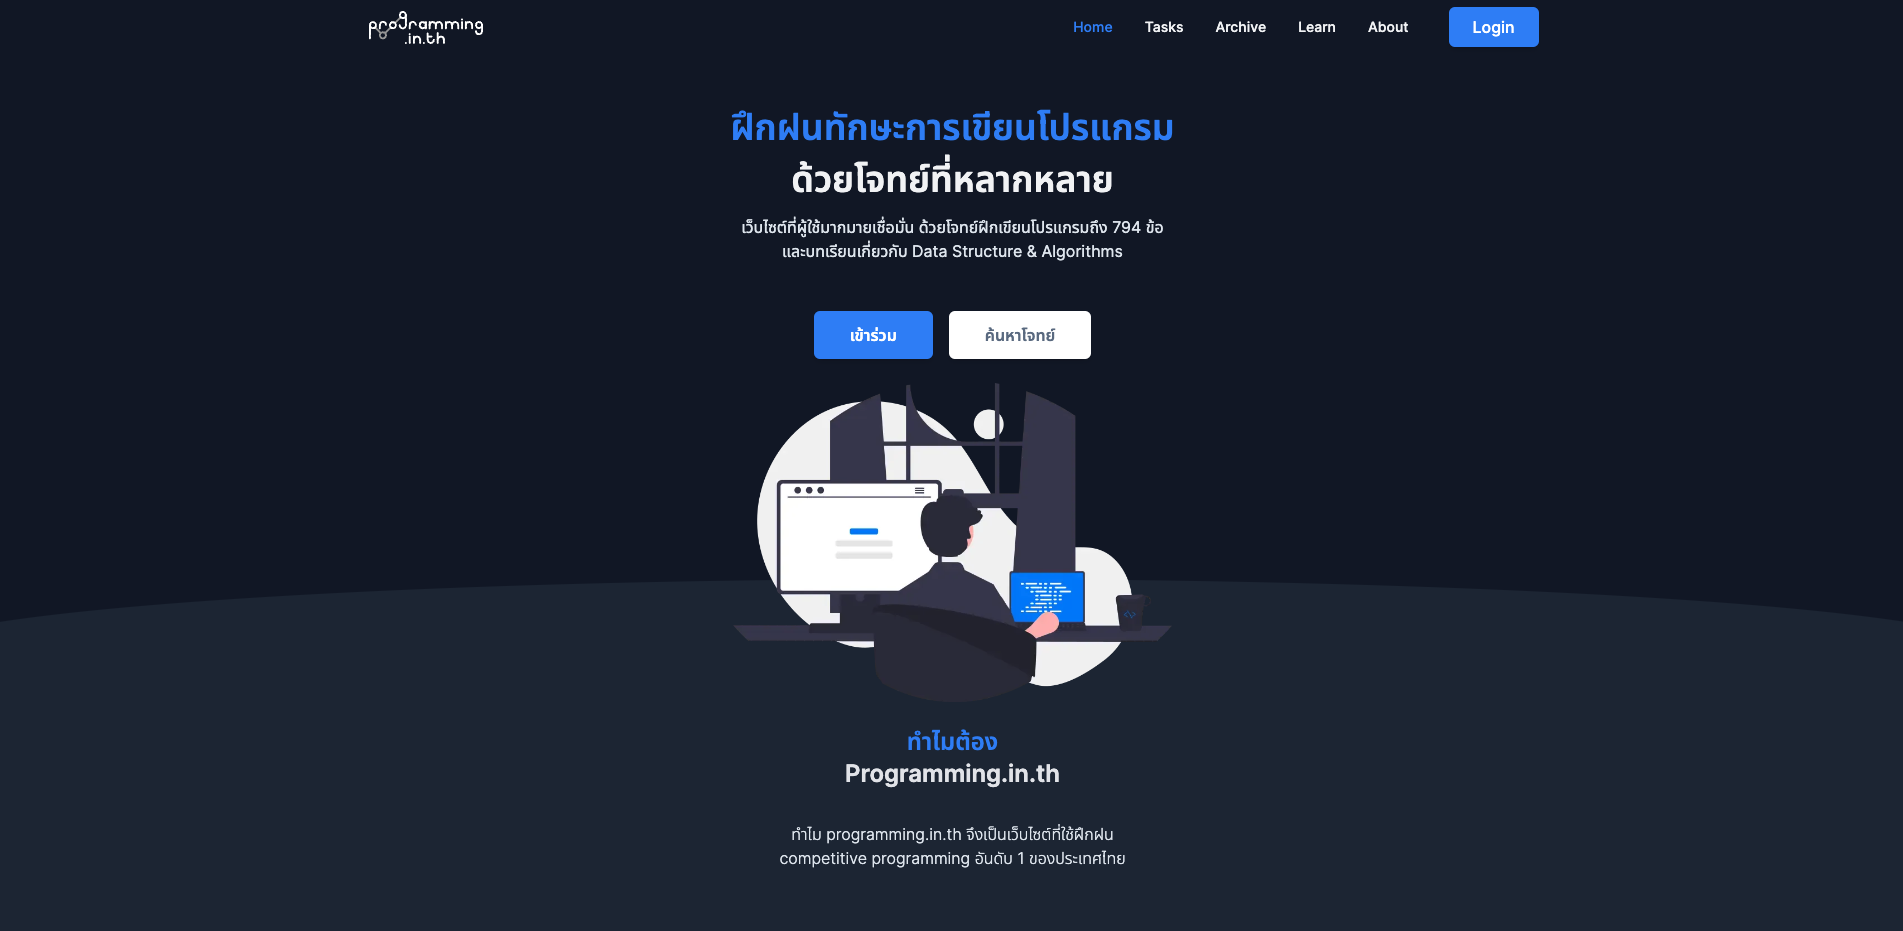
\includegraphics[width=7cm]{figure/literature/current-ipst.png}
    \label{fig:ipst-page-new}
  }
  \caption[หน้าหลักของ IPST Program Grader]{หน้าหลักของ IPST Program Grader}
  \label{fig:ipst-page}
\end{figure}
\thaijustify{
  เว็บไซต์นี้มีฐานข้อมูลโจทย์ปัญหาที่แต่งโดยทางสสวท. ที่ผู้ใช้สามารถกดเลือกเข้าไปทำข้อไหนก็ได้ มีระบบสมัครสมาชิก และมีแหล่งเรียนรู้เพิ่มเติม (Learning resource) สำหรับให้ผู้ใช้ได้เข้าอ่านทำความเข้าใจและเรียนรู้การเขียนโปรแกรม
}
\thaijustify{
  เว็บไซต์ดังกล่าวเป็นหนึ่งในแรงบันดาลใจ ต้นฉบับความคิดและต้นแบบซอฟต์แวร์ที่ \textit{Program Grading System}~\cite{nattawat20pgs} ใช้เป็นตัวอย่างในเชิงของแนวคิดในการออกแบบซอฟต์แวร์
}
\thaijustify{
  ใน \textit{Jamlongrad et al.}~\cite{nattawat20pgs} ได้มีการวิเคราะห์ สรุปข้อดีและข้อเสียของระบบ แต่เนื่องจากเว็บไซต์ได้มีการเปลี่ยนแปลงในรอบปีที่ผ่านมา คณะผู้จัดทำก็ได้ไปสำรวจการทำงานเว็บไซต์ใหม่อีกรอบหนึ่ง แล้วนำผลสำรวจมาสรุปรวบยอดกับในรายงานดังกล่าว สรุปเป็นผลเป็นตาราง~\ref{tbl:ipst-pro-cons} ดังต่อไปนี้
}
\begin{table}[H]
  \centering
  \caption{ข้อดีและข้อเสียของระบบ IPST Grader}
  \label{tbl:ipst-pro-cons}
  \begin{tabular}{p{1cm}|p{6cm}|p{6cm}} \hline\hline
    ข้อที่ & ข้อดี                                                                                   & ข้อเสีย                                                                                                                              \\
    \hline\hline
    1.  & \RaggedRight{เว็บไซต์มีระบบการตรวจและประเมินผลโปรแกรมที่รวดเร็ว ผู้ใช้สามารถรับรู้ผลได้ทันที}\par     & \RaggedRight{เว็บไซต์ไม่สามารถจะใช้งานเครือข่ายเฉพาะได้ เพราะเว็บไซต์ดังกล่าวอยู่ในเครือข่ายสาธารณะ ทำให้เว็บไซต์นี้ไม่สามารถนำมาใช้ในการแข่งขันภายในได้}\par \\ \hline
    2.  & \RaggedRight{ส่วนประสานผู้ใช้ถูกออกแบบมาอย่างดี เพื่อความสะดวกสบายของผู้ใช้}\par                  & \RaggedRight{ไม่มีระบบสื่อสาร ไม่มีระบบกระทู้สนทนา ไม่มีช่องทางการสื่อสารให้ผู้ใช้ได้คุยปรึกษากันเรื่องโจทย์}\par                                          \\ \hline
    3.  & \RaggedRight{เว็บไซต์มีโจทย์ปัญหาที่หลากหลาย แต่งแต่ระดับง่ายสุด ไปยังระดับการแข่งขันระดับนานาชาติ}\par & \RaggedRight{ผู้ใช้ไม่สามารถเพิ่มโจทย์ปัญหาเองได้ โจทย์ปัญหาถูกควบคุมและเพิ่มโดยผู้ดูแลเว็บเท่านั้น}\par                                                 \\ \hline
    4.  & \RaggedRight{เว็บไซต์มีระบบจัดหมวดหมู่โจทย์ปัญหา ทำให้ผู้ใช้หาโจทย์ปัญหาที่ต้องการทำได้ง่าย}\par           &                                                                                                                                    \\
    \hline\hline
  \end{tabular}
\end{table}
% IMPROVED TO TABLE
% \begin{itemize}
%     \item \textbf{ข้อดี}
%     \begin{enumerate}
%         \item เว็บไซต์มีระบบการตรวจและประเมินผลโปรแกรมที่รวดเร็ว ผู้ใช้สามารถรับรู้ผลได้ทันที
%         \item ส่วนประสานผู้ใช้ (user interface) ถูกออกแบบมาอย่างดี เพื่อความสะดวกสบายของผู้ใช้
%         \item เว็บไซต์มีโจทย์ปัญหาที่หลากหลาย แต่งแต่ระดับง่ายสุด ไปยังระดับการแข่งขันระดับนานาชาติ
%         \item เว็บไซต์มีระบบจัดหมวดหมู่โจทย์ปัญหา ทำให้ผู้ใช้หาโจทย์ปัญหาที่ต้องการทำได้ง่าย
%     \end{enumerate}
%     \item \textbf{ข้อเสีย}
%     \begin{enumerate}
%         \item เว็บไซต์ไม่สามารถจะใช้งานเครือข่ายเฉพาะได้ เพราะเว็บไซต์ดังกล่าวอยู่ในเครือข่ายสาธารณะ ทำให้เว็บไซต์นี้ไม่สามารถนำมาใช้ในการแข่งขันภายในได้
%         \item ไม่มีระบบสื่อสาร ไม่มีระบบกระทู้สนทนา ไม่มีช่องทางการสื่อสารให้ผู้ใช้ได้คุยปรึกษากันเรื่องโจทย์
%         \item ผู้ใช้ไม่สามารถเพิ่มโจทย์ปัญหาเองได้ โจทย์ปัญหาถูกควบคุมและเพิ่มโดยผู้ดูแลเว็บเท่านั้น
%     \end{enumerate}
% \end{itemize}
\subsection{Codeforces}
\thaijustify{
  ซอฟต์แวร์ \href{https://codeforces.com}{Codeforces} เป็นเว็บไซต์แอปพลิเคชัน ที่สร้างขึ้นโปรแกรมเมอร์ที่ชื่อ \textit{Mike Mirzayanov}~\cite{codeforces} ในปี 2553 สร้างขึ้นมาด้วยวัตถุประสงค์เดียวกับ programming.in.th เพื่อให้ผู้ใช้สามารถเข้ามาฝึกฝนทักษะการเขียนโปรแกรม เรียนรู้การเขียนโปรแกรม
}
\thaijustify{
  เว็บไซต์นี้มีฐานข้อมูลโจทย์ปัญหาที่แต่งโดยทางผู้ดูแลเว็บไซต์เหมือนกับเว็บไซต์ programming.in.th ที่ผู้ใช้สามารถเข้าไปเลือกทำได้ แต่ข้อแตกต่างที่ทำให้เว็บไซต์นี้แตกต่างคือระบบการแข่งขัน ระบบตารางคะแนน
}
\begin{figure}[H]
  \centering
  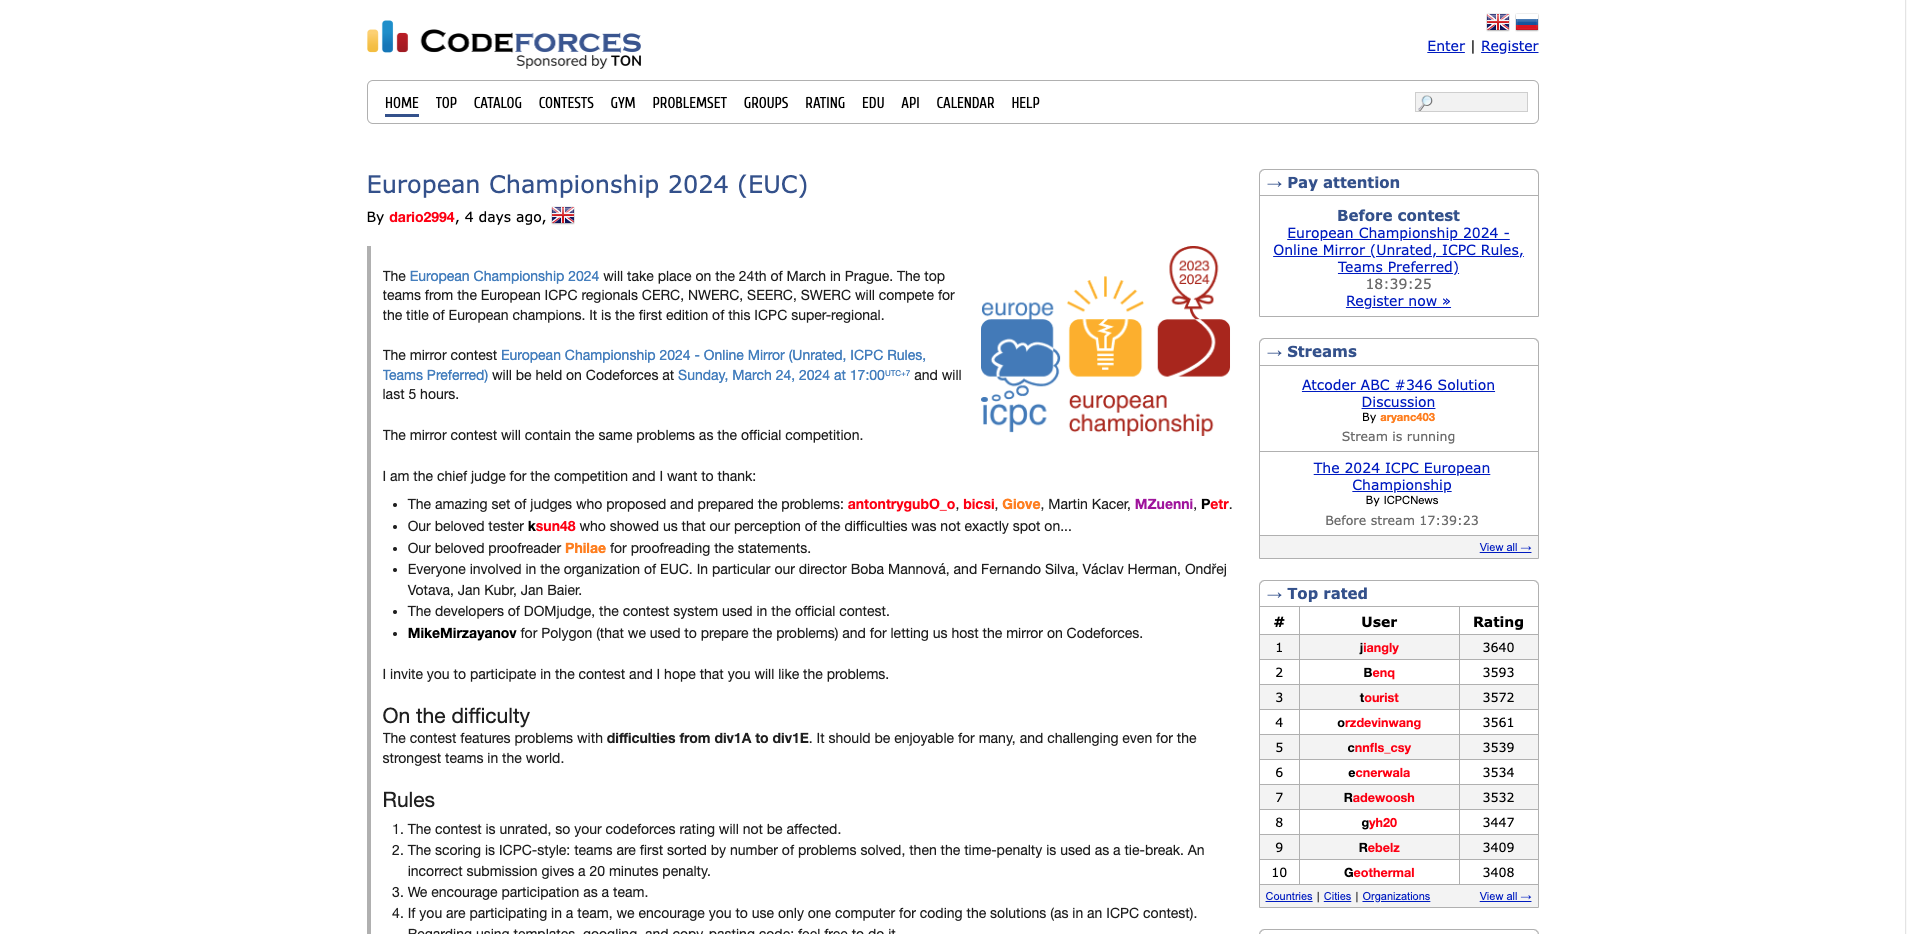
\includegraphics[width=10cm]{figure/literature/codeforces.png}
  \caption[หน้าหลักของ Codeforces]{หน้าหลักของ Codeforces ณ วันที่ 31 สิงหาคม 2566~\cite{codeforces}}\label{fig:codeforces-page}
\end{figure}
\thaijustify{
  เว็บไซต์นี้มีการจัดการแข่งขันเป็นช่วง ๆ มีการจัดลำดับผู้เข้าแข่งขันด้วยระบบการตรวจและประเมินโปรแกรม คะแนนจะมากน้อยขึ้นกับสองปัจจัยหลัก ประกอบด้วยความถูกต้อง (Correction) และประสิทธิภาพ (Performance or efficiency) โปรแกรมที่ให้คำตอบที่ถูกต้อง ใช้ทรัพยากรน้อย และใช้เวลาหาคำตอบน้อยจะได้คะแนนสูง ผู้เข้าแข่งขันคนไหนที่สามารถแก้โจทย์ปัญหาได้ถูกต้องและมีประสิทธิภาพ มากที่สุดในเวลาที่จำกัดจะถือเป็นผู้ชนะ
}
\thaijustify{
  จาก~\cite{nattawat20pgs} ก็ได้นำเอาซอฟต์แวร์ตัวนี้ไปทำการวิเคราะห์ และคัดสรรเลือกคุณลักษณะเด่นไปพัฒนาเช่นเดียวกัน โดยกลุ่มนักศึกษาเจ้าของโครงการดังกล่าวก็ได้สรุปข้อดีและข้อเสียของซอฟต์แวร์ Codeforces ไว้ตามตาราง~\ref{tbl:codeforces-pro-cons} ดังต่อไปนี้
}
\begin{table}[H]
  \centering
  \caption{ข้อดีและข้อเสียของระบบ Codeforces}\label{tbl:codeforces-pro-cons}
  \begin{tabular}{p{1cm}|p{6cm}|p{6cm}} \hline\hline
    ข้อที่ & ข้อดี                                                                                                                            & ข้อเสีย                                                                                                                              \\
    \hline\hline
    1.  & \RaggedRight{เว็บไซต์มีระบบการตรวจและประเมินผลโปรแกรมที่รวดเร็ว ผู้ใช้สามารถรับรู้ผลได้ทันที}\par                                              & \RaggedRight{เว็บไซต์ไม่สามารถจะใช้งานเครือข่ายเฉพาะได้ เพราะเว็บไซต์ดังกล่าวอยู่ในเครือข่ายสาธารณะ ทำให้เว็บไซต์นี้ไม่สามารถนำมาใช้ในการแข่งขันภายในได้}\par \\ \hline
    2.  & \RaggedRight{มีระบบตารางคะแนน มีการจัดอันดับคะแนนผู้ใช้ ส่งเสริมให้ผู้ใช้พัฒนาตนเอง ส่งเสริมให้เกิดการแข่งขัน}\par                                  & \RaggedRight{ส่วนประสานผู้ใช้ออกแบบมาไม่ดี ไม่สะดวกต่อการใช้งาน}\par                                                                        \\ \hline
    3.  & \RaggedRight{มีระบบสื่อสาร มีระบบกระทู้สนทนา มีช่องทางการสื่อสารให้ผู้ใช้ได้คุยปรึกษากันเรื่องโจทย์ มีช่องทางประกาศประชาสัมพันธ์ข่าวสารและผลการแข่งขัน}\par & \RaggedRight{}\par                                                                                                                 \\ \hline
    4.  & \RaggedRight{ผู้ใช้สามารถเพิ่มโจทย์ปัญหาเองได้ ถ้าหากได้รับอนุญาต รับบทบาทเป็นผู้ดูแลระบบจากเจ้าของเว็บไซต์}\par                                   & \RaggedRight{}\par                                                                                                                 \\
    \hline\hline
  \end{tabular}
\end{table}
% IMPROVED TO TABLE
% \begin{itemize}
%     \item \textbf{ข้อดี}
%     \begin{enumerate}
%         \item เว็บไซต์มีระบบการตรวจและประเมินผลโปรแกรมที่รวดเร็ว ผู้ใช้สามารถรับรู้ผลได้ทันที
%         \item มีระบบตารางคะแนน มีการจัดอันดับคะแนนผู้ใช้ ส่งเสริมให้ผู้ใช้พัฒนาตนเอง ส่งเสริมให้เกิดการแข่งขัน
%         \item เว็บไซต์มีโจทย์ปัญหาที่หลากหลาย จัดเป็นหมวดหมู่เรียบร้อย จัดระดับความยากง่าย ผู้ใช้สามารถหาโจทย์ปัญหาที่ต้องการทำได้ง่าย
%         \item มีระบบสื่อสาร มีระบบกระทู้สนทนา มีช่องทางการสื่อสารให้ผู้ใช้ได้คุยปรึกษากันเรื่องโจทย์ มีช่องทางประกาศประชาสัมพันธ์ข่าวสารและผลการแข่งขัน
%     \end{enumerate}
%     \item \textbf{ข้อเสีย}
%     \begin{enumerate}
%         \item เว็บไซต์ไม่สามารถจะใช้งานเครือข่ายเฉพาะได้ เว็บไซต์อยู่ในเครือข่ายสาธารณะ เว็บไซต์นี้ไม่สามารถนำมาใช้ในการแข่งขันที่มีการจำกัดการเข้าถึงข้อมูลออนไลน์
%         \item ส่วนประสานผู้ใช้ (User Interface) ออกแบบมาไม่ดี ไม่สะดวกต่อการใช้งาน
%     \end{enumerate}
% \end{itemize}
\pagebreak
% TODO: Add LeetCode and other program graders
% \subsection{LeetCode}
% \pagebreak
\subsection{Programming Grader System}
\thaijustify{
  ซอฟต์แวร์ PGS หรือชื่อเต็มของโครงการ การพัฒนาระบบตรวจสอบผลลัพธ์ของโจทย์ปัญหาจากชัดซอร์สโค้ดเพื่อการเรียนการสอน (ภาษาอังกฤษคือ Programming Grader System) เป็นโครงงานพัฒนาซอฟต์แวร์ของนักศึกษาชั้นปีสี่ในรายวิชา CPE401 ปีการศึกษา 2563~\cite{nattawat20pgs}
}
\thaijustify{
  โดยซอฟต์แวร์ดังกล่าวถูกตั้งขึ้นมาเพื่อแก้ปัญหาการตรวจงานที่ยุ่งยาก ในรายวิชาการเรียนการสอนเขียนโปรแกรมภาษาคอมพิวเตอร์ ซึ่งเป็นปัญหาเดียวกันกับปัญหาที่คณะผู้จัดทำมุ่งมั่นได้ตั้งไว้ และมุ่งมั่นจะแก้ในโครงการนี้ โดยเว็บไซต์นี้ถูกสร้างและออกแบบ โดยนำเอาข้อดีและข้อเสียของเว็บไซต์ IPST Program Grader และ Codeforces โดยนักศึกษาปีสี่กลุ่มดังกล่าวได้ สำรวจและวิเคราะห์ระบบการทำงานและคุณลักษณะ (Feature) ของทั้งสองเว็บแล้วคัดสรรนำคุณลักษณะที่เด่นและดีมาใช้พัฒนาลงในซอฟต์แวร์ PGS
}
\begin{figure}[H]
  \centering
  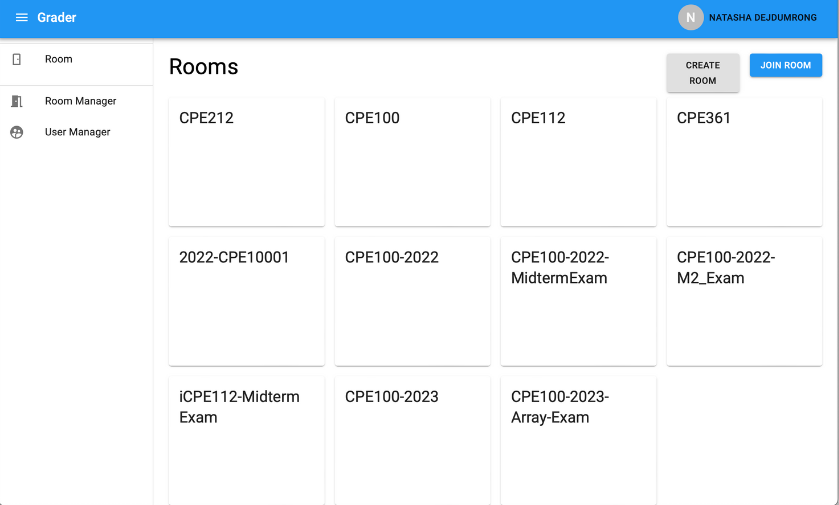
\includegraphics[width=9cm]{figure/literature/pgs.png}
  \caption[หน้าหลักของ Program Grading System]{หน้าหลักของ Program Grading System หรือ PGS ณ วันที่ 9 ตุลาคม 2566}\label{fig:pgs-page}
\end{figure}

\thaijustify{
  เนื่องจากโครงงานปริญญานิพนธ์~\cite{nattawat20pgs} มีปัญหาและเค้าโครงของโครงการที่ใกล้เคียงกับโครงการของคณะผู้จัดทำมากที่สุด เป็นเหตุให้คณะผู้จัดทำตัดสินใจนำเอาโครงการนี้มาเป็นซอฟต์แวร์ต้นแบบ ที่ซอฟต์แวร์กลุ่มคณะผู้จัดทำจะใช้เป็นแหล่งอ้างอิงหลัก
}
\thaijustify{
  หลังจากทางคณะผู้จัดทำได้ไปทำการสำรวจและวิเคราะห์คุณลักษณะของซอฟต์แวร์ ทางคณะผู้จัดทำสามารถที่จะสรุปข้อดีและข้อเสียของระบบ PGS ได้ตามตาราง~\ref{tbl:pgs-pro-cons-1} ดังต่อไปนี้
}

\begin{longtable}{p{1cm}|p{6cm}|p{6cm}}
  % First header
  \caption{ข้อดีและข้อเสียของระบบ Program Grader System}\label{tbl:pgs-pro-cons-1}                                                                                                                                                                                                             \\ % First caption
  \hline\hline
  ข้อที่ & ข้อดี                                                                                                                       & ข้อเสีย                                                                                                                                                  \\
  \hline\hline
  \endfirsthead
  % Re-occurring header
  \caption[]{ข้อดีและข้อเสียของระบบ Program Grader System (ต่อ)}                                                                                                                                                                                                                                \\ % Cont. caption
  \hline\hline
  ข้อที่ & ข้อดี                                                                                                                       & ข้อเสีย                                                                                                                                                  \\
  \hline\hline
  \endhead
  % First footer
  \endfoot
  % Last footer
  \hline
  \endlastfoot
  % Body
  1.  & \RaggedRight{เว็บไซต์มีระบบการตรวจและประเมินผลโปรแกรมที่เร็วพอสมควร}\par                                                         & \RaggedRight{การประเมินผลโปรแกรมของเว็บไซต์ไม่มีความคงที่ ตรวจให้ผลทันทีบ้าง ให้ผลช้าบ้าง}\par                                                                       \\ \hline
  2.  & \RaggedRight{มีระบบตารางคะแนน มีการจัดอันดับคะแนนผู้ใช้ ส่งเสริมให้ผู้ใช้พัฒนาตนเอง ส่งเสริมให้เกิดการแข่งขัน}\par                             & \RaggedRight{คะแนนที่ได้บันทึกไว้บนตารางคะแนน ไม่สามารถจะนำออกมาเป็นไฟล์ excel สำหรับตรวจและประเมินได้}\par                                                          \\ \hline
  3.  & \RaggedRight{เว็บไซต์มีโจทย์ปัญหาที่หลากหลาย จัดเป็นหมวดหมู่ตามห้องเรียนเรียบร้อย จัดระดับความยากง่าย ผู้ใช้สามารถหาโจทย์ปัญหาที่ต้องการทำได้ง่าย}\par & \RaggedRight{เว็บไซต์ไม่มีระบบสมัครสมาชิก สร้างบัญชีเอง ฉะนั้นจะต้องให้เจ้าของระบบเป็นคนสร้างบัญชีให้ทุกๆ ครั้ง}\par                                                         \\ \hline
  4.  & \RaggedRight{มีระบบการแสดงความเห็นในแต่ละชุดคำสั่งที่ผู้ใช้ได้ส่งขึ้นมา ที่อาจารย์ผู้สอนหรือผู้ดูแลสามารถมาให้ความเห็นหรือความแนะนำได้}\par             & \RaggedRight{การเพิ่มหรือแก้ไขโจทย์นั้นยากลำบากและไม่สะดวก ไม่สามารถจะนำชุดโจทย์ ชุดเทสเคสมาเพิ่มพร้อมกันได้ ต้องทำการเพิ่มทีละรายการ}\par                                     \\ \hline
  5.  & \RaggedRight{ผู้ใช้ที่สามารถเพิ่มโจทย์ปัญหาเองได้ หากได้รับอนุญาตจากผู้ดูแลเว็บไซต์}\par                                                    & \RaggedRight{ในการตรวจชุดคำสั่ง ต้องคัดลอก (copy) จากบนเว็บไซต์มาวาง (paste) บน IDE บนเครื่อง ไม่สามารถที่จะนำชุดคำสั่งออกจากเว็บไซต์เป็นไฟล์ (export file) ออกมาตรวจได้}\par \\ \hline
  6.  & \RaggedRight{}\par                                                                                                        & \RaggedRight{ส่วนประสานงานผู้ใช้ ไม่เป็นมิตรและไม่สะดวกต่อผู้ใช้งาน}\par                                                                                           \\ \hline
\end{longtable}

% IMPROVED TO TABLE
% \begin{itemize}
%     \item \textbf{ข้อดี}
%     \begin{enumerate}
%         \item เว็บไซต์มีระบบการตรวจและประเมินผลโปรแกรมที่เร็วพอสมควร ผู้ใช้สามารถรับรู้ผลได้หลังจากส่งชุดคำสั่งขึ้นตรวจ
%         \item มีระบบตารางคะแนน มีการจัดอันดับคะแนนผู้ใช้ ส่งเสริมให้ผู้ใช้พัฒนาตนเอง ส่งเสริมให้เกิดการแข่งขัน
%         \item เว็บไซต์มีโจทย์ปัญหาที่หลากหลาย จัดเป็นหมวดหมู่ตามห้องเรียนเรียบร้อย จัดระดับความยากง่าย ผู้ใช้สามารถหาโจทย์ปัญหาที่ต้องการทำได้ง่าย
%         \item มีระบบการแสดงความเห็นในแต่ละชุดคำสั่งที่ผู้ใช้ได้ส่งขึ้นมา ที่อาจารย์ผู้สอนหรือผู้ดูแลสามารถมาให้ความเห็นหรือความแนะนำได้
%         \item ผู้ใช้ที่สามารถเพิ่มโจทย์ปัญหาเองได้ หากได้รับอนุญาตจากผู้ดูแลเว็บไซต์
%     \end{enumerate}
%     \item \textbf{ข้อเสีย}
%     \begin{enumerate}
%         \item เว็บไซต์ไม่สามารถรองรับการทำงานของผู้ใช้หลาย ๆ คน พร้อมกันได้
%         \item ส่วนประสานงานผู้ใช้ (หรือ User Interface) ไม่เป็นมิตร ไม่สะดวกต่อผู้ใช้
%         \item การเพิ่มหรือแก้ไขโจทย์นั้นยากลำบากและไม่สะดวก ไม่สามารถจะนำชุดโจทย์ ชุดเทสเคสมาเพิ่มพร้อมกันได้ ต้องทำการเพิ่มทีละรายการ
%         \item ในการตรวจชุดคำสั่ง ต้องคัดลอก (copy) จากบนเว็บไซต์มาวาง (paste) บน IDE บนเครื่อง ไม่สามารถที่จะนำชุดคำสั่งออกจากเว็บไซต์เป็นไฟล์ (export file) ออกมาตรวจได้
%         \item คะแนนที่ได้บันทึกไว้บนตารางคะแนน ไม่สามารถจะนำออกมาเป็นไฟล์ excel สำหรับตรวจและประเมินได้
%     \end{enumerate}
% \end{itemize}

\section{ภาษาคอมพิวเตอร์เเละเทคโนโลยี}
\thaijustify{
  หลังจากที่ได้ค้นคว้าหาแนวคิด ทฤษฎีและหลักการ รวมไปถึงซอฟต์แวร์ที่จะนำมาใช้อ้างอิงเป็นต้นแบบให้กับซอฟต์แวร์ที่ทางกลุ่มจะพัฒนาขึ้นมาเป็นที่เรียบร้อยแล้ว ในส่วนหัวข้อถัดไปคณะผู้จัดทำจะบรรยายและอธิบายถึงลักษณะ ความสามารถและหน้าทีของเครื่องมือ เทคโนโลยีและซอฟต์แวร์ประกอบแต่ละอย่าง พร้อมทั้งอธิบายถึงเหตุผลที่เครื่องมือ เทคโนโลยีและซอฟต์แวร์ดังกล่าวนั้นเหมาะสมที่จะนำมาใช้ในขั้นพัฒนาซอฟต์แวร์โครงการ
}
\subsection{ภาษาคอมพิวเตอร์}
\thaijustify{
  เนื่องด้วยโครงการนี้เป็นโครงการพัฒนาซอฟต์แวร์ จึงต้องมีการเขียนโปรแกรมขึ้นมาเพื่อสร้างเป็นระบบซอฟต์แวร์ คณะผู้จัดทำจึงได้ไปศึกษาหาภาษาคอมพิวเตอร์ที่คิดว่าเหมาะสมกับ จุดประสงค์และการทำงานที่คาดหวังไว้ของซอฟต์แวร์โครงการ
}
\subsubsection{ภาษา Go}
\thaijustify{
  ภาษา Go หรือที่รู้จักกันอย่างแพร่หลายว่า Golang เป็นภาษาโปรแกรมเปิดต้นทางที่พัฒนาโดยทีมนักพัฒนาซอฟต์แวร์ที่ Google โดยรวมถึง Robert Griesemer, Rob Pike, และ Ken Thompson เหล่านักพัฒนาที่ในไม่กี่ทศวรรษก่อน พัฒนาภาษา C ขึ้นมา ภาษา Go นั้นถูกออกแบบขึ้น เพื่อแก้ไขข้อจำกัดของภาษาโปรแกรมเดิมที่มีอยู่แล้วทั้งในด้านประสิทธิภาพ (Efficiency) ความเรียบง่าย (Simplicity) และการสนับสนุนการทำงานพร้อมกัน (Concurrency มีไวยากรณ์ (Syntax) ที่กระชับ การกำหนดประเภท (Type) ที่แข็งแรง พร้อมทั้งระบบจัดการทรัพยากรขยะของโปรแกรม (Garbage Collection) ที่มีประสิทธิภาพ~\cite{pike12go, donovan15go}
}
\thaijustify{
  จากความเห็นของ \textit{Pike R.} ใน~\cite{pike12go, pike12godev} หนึ่งในลักษณะที่ดีเด่น Go คือการให้ความสำคัญกับความเรียบง่ายและความอ่านง่าย ทำให้เป็นทางเลือกที่ยอดเยี่ยมสำหรับทั้งผู้เริ่มต้นและนักพัฒนาที่มีประสบการณ์มาก มันนำเสนอแนวทางที่มีความเรียบง่าย ป้องกันความซับซ้อนที่ไม่จำเป็น และมีไวยากรณ์ที่ถูกต้องและโดดเด่น ภาษานี้รวมถึงคุณสมบัติที่สนับสนุนการทำงานพร้อมกันที่ซึ่งช่วยให้นักพัฒนาสามารถเขียนแอปพลิเคชันที่มีประสิทธิภาพและมีขนาดใหญ่ได้
}
\thaijustify{
  การทำงานพร้อมกันหรือ Concurrency ก็เป็นแข็งสำคัญของ Go อย่างหนึ่ง การทำ Concurrency ในภาษา ทำผ่าน Channel และ GoRoutines ซึ่งเป็น Thread ที่ Light-weighted ทำให้สามารถสร้างโปรแกรมที่ทำงานพร้อมกันได้โดยไม่มีความซับซ้อน~\cite{donovan15go}
}
\thaijustify{
  เนื่องจาก ภาษา Go นั้นกำลังได้รับความนิยมในหลาย ๆ ด้าน ณ ปีการศึกษานี้เช่น การสร้างหรือพัฒนาเว็บไซต์ เว็บแอปพลิเคชัน, การสร้างระบบบริการ Cloud, การสร้างซอฟต์แวร์ระบบที่มีประสิทธิภาพ เป็นต้น ภาษา Go เป็นภาษาที่ใช้งานง่าน และสามารถรันโปรแกรมที่อาศัยการทำงานหรือประมวลแบบ Parallel และ Concurrent~\cite{golangorg} ด้วยเหตุนี้บริษัทใหญ่หลายบริษัทในยุคใหม่ที่มีระบบซอฟต์แวร์ที่ใหญ่ จึงนิยมใช้ภาษาดังกล่าว แล้วเนื่องด้วยสมาชิกในกลุ่มคณะผู้จัดทำได้มีโอกาสไปฝึกงานบริษัทที่ใช้ภาษาดังกล่าว จึงเห็นเป็นโอกาสนำความรู้และความเข้าใจมาประยุกต์ในโครงงานนี้
}
\subsubsection{ภาษา JavaScript}
\thaijustify{
  ภาษา JavaScript เป็นภาษาโปรแกรมที่หลากหลายและใช้กันอย่างแพร่หลาย โดยหลักแล้วเป็นที่รู้จักจากบทบาทในการพัฒนาเว็บ พัฒนาโดย Netscape และได้กลายเป็นองค์ประกอบพื้นฐานสำหรับการสร้างเว็บไซต์เชิงโต้ตอบและไดนามิก JavaScript ถูกดำเนินการบนฝั่งไคลเอ็นต์ ทำให้เบราว์เซอร์สามารถจัดการ Document object model (หรือเรียกโดยชื่อย่อว่า DOM) และตอบสนองต่อการโต้ตอบของผู้ใช้ ไวยากรณ์ของมันได้รับอิทธิพลจาก Java ทำให้นักพัฒนาที่คุ้นเคยกับภาษา C สามารถเข้าถึงได้~\cite{flanagan20js}
}
\thaijustify{
  ข้อดีอย่างหนึ่งที่โดดเด่นของ JavaScript คือการแพร่หลายไปทั่วเว็บเบราว์เซอร์ เนื่องจากได้รับการสนับสนุนโดยเบราว์เซอร์หลักๆ ทั้งหมด เช่น Chrome, Firefox และ Safari การนำไปใช้อย่างแพร่หลายนี้ทำให้มั่นใจได้ว่าแอปพลิเคชันที่ขับเคลื่อนด้วย JavaScript สามารถเข้าถึงผู้ชมจำนวนมากได้โดยไม่มีปัญหาเรื่องความเข้ากันได้~\cite{flanagan20js} นอกจากนี้ JavaScript ยังเปิดใช้งานการเขียนโปรแกรมแบบอะซิงโครนัสผ่านคุณสมบัติเช่นการโทรกลับและคำสัญญา ซึ่งอำนวยความสะดวกในการพัฒนาแอปพลิเคชันเว็บที่ตอบสนองและมีประสิทธิภาพ ลักษณะที่ไม่ซับซ้อนของภาษาช่วยให้โหลดหน้าเว็บได้เร็วขึ้น ปรับปรุงประสบการณ์ผู้ใช้โดยรวม~\cite{crockford08js}
}
\thaijustify{
  อย่างไรก็ตาม JavaScript ก็มีข้อเสียอยู่เช่นกัน ข้อเสียเปรียบที่สำคัญประการหนึ่งคือมีโอกาสเกิดช่องโหว่ด้านความปลอดภัย โดยเฉพาะอย่างยิ่งเมื่อดำเนินการบนฝั่งไคลเอ็นต์ เนื่องจากซอร์สโค้ดสามารถมองเห็นได้โดยผู้ใช้ จึงสามารถจัดการเพื่อจุดประสงค์ที่เป็นอันตรายได้ ซึ่งนำไปสู่ความเสี่ยงด้านความปลอดภัย เช่น การโจมตี Cross-Site Scripting (XSS)~\cite{flanagan20js} นอกจากนี้ การขาดการพิมพ์ที่ชัดเจนอาจทำให้การตรวจจับข้อผิดพลาดบางประเภทในระหว่างการพัฒนาเป็นเรื่องยาก ซึ่งอาจนำไปสู่ปัญหารันไทม์ (Runtime) ที่ยากต่อการวินิจฉัยและแก้ไข (Difficult to diagnose and fix)~\cite{crockford08js}
}
\thaijustify{
  แม้จะมีข้อจำกัด JavaScript ยังคงเป็นส่วนสำคัญของการพัฒนาเว็บยุคใหม่ เนื่องจากความสามารถรอบด้านและระบบนิเวศที่กว้างขวางของไลบรารี (Library) และเฟรมเวิร์ก (Framework) เช่น React และ Angular ที่สร้างขึ้นจากมัน~\cite{flanagan20js} การพัฒนาอย่างต่อเนื่องของภาษาและความพยายามในการแก้ไขข้อบกพร่องมีส่วนช่วยให้ภาษามีความเกี่ยวข้องอย่างต่อเนื่องในภูมิทัศน์แบบไดนามิกของการพัฒนาเว็บ~\cite{crockford08js}
}
\thaijustify{
  แม้ภาษา JavaScript จะเป็นภาษาที่นิยมสำหรับการเขียนส่วนประสานงานผู้ใช้ แต่ทางคณะผู้จัดทำตัดสินใจไม่เลือกที่จะใช้ภาษา JavaScript เพราะข้อผิดพลาดและข้อเสียของภาษาหลายอย่าง ไม่สามารถที่จะมองข้ามไปได้และสามารถที่จะสร้างเป็นอุปสรรคสำหรับงานโครงงานของกลุ่ม อาทิเช่นการนิยามประเภทของตัวแปร ของ JavaScript (Type-defining) ที่กำกวมและไม่เป็นระเบียบ อาจทำให้การตรวจสอบหาข้อผิดพลาดของการทำงานตรงส่วนประสานงานผู้ใช้ที่เขียนด้วยภาษาดังกล่าว ตรวจสอบหาปัญหาได้ยาก
}
\thaijustify{
  ด้วยข้อเสียดังกล่าว คณะผู้จัดทำไม่ได้คิดจะนำภาษา JavaScript มาใช้เป็นภาษาหลักของหน้าเว็บไซต์ แต่เลือกภาษาที่ถูกสร้างมาเพื่อแก้จุดอ่อนของภาษา JavaScript โดยเฉพาะปัญหาความกำกวมและความวุ่นวายของประเภทตัวแปร (Ambiguous and non-strict type) ที่เรียกว่า TypeScript ซึ่งจะอธิบายในหัวข้อถัดไป ดังนั้นภาษา JavaScript จะถูกใช้ในโครงงานนี้ เพียงเพื่อเป็นภาษาสั่งการหรือตั้งค่า สำหรับสนับสนุนงานด้านการสร้าง (Build) ซอฟต์แวร์กำลังพัฒนา (Development Build) เขียนด้วยภาษา TypeScript ไปเป็นซอฟต์แวร์พร้อมใช้งาน (Production Build) ในภาษา JavaScript
}
\subsubsection{ภาษา TypeScript}
\thaijustify{
  ภาษา TypeScript เป็นชุดที่เหนือกว่าของ JavaScript ที่แนะนำการพิมพ์แบบคงที่ให้กับภาษา ช่วยให้นักพัฒนาซอฟต์แวร์มีเครื่องมือที่ได้รับการปรับปรุง การบำรุงรักษาโค้ดที่ได้รับการปรับปรุง และการตรวจจับข้อผิดพลาดตั้งแต่เนิ่นๆ ในระหว่างการพัฒนา TypeScript เป็นโอเพ่นซอร์สและดูแลโดย Microsoft และคอมไพล์เป็น JavaScript ธรรมดา ทำให้เข้ากันได้กับโค้ดเบส JavaScript ที่มีอยู่~\cite{hejlsbergts, microsoftts}
}
\thaijustify{
  ข้อดีหลักประการหนึ่งของ TypeScript คือระบบการพิมพ์แบบคงที่ ด้วยการรวมคำอธิบายประกอบประเภท นักพัฒนาสามารถกำหนดประเภทของตัวแปร พารามิเตอร์ฟังก์ชัน และค่าที่ส่งคืนที่คาดเดาได้ (Deterministic behavior) ซึ่งจะช่วยตรวจจับข้อผิดพลาดที่เกี่ยวข้องกับประเภทในระหว่างการพัฒนา ลดจุดบกพร่องหรือข้อผิดพลาด พร้อมปรับปรุงคุณภาพของโปรแกรมไปด้วย~\cite{cherny19ts, microsoftts}
}
\thaijustify{
  นอกจากนี้ TypeScript ยังรองรับฟีเจอร์ ECMAScript สมัยใหม่ ทำให้สร้างโค้ดที่มีทั้ง Solubility และ Maintainability ได้สำหรับแอปพลิเคชันขนาดใหญ่ ภาษา TypeScript ให้การสนับสนุนหลักการเขียนโปรแกรมเชิงวัตถุ (Object-Oriented programming) รวมถึงคลาสและอินเทอร์เฟซ (Class and Interface) อำนวยความสะดวกในการพัฒนาซอฟต์แวร์ที่แข็งแกร่งและมีโครงสร้าง~\cite{hejlsbergts}
}
\thaijustify{
  อย่างไรก็ตาม TypeScript ก็มีข้อเสียเช่นกัน ข้อเสียเปรียบประการหนึ่งคือเรียนรู้ใช้งานยาก โดยเฉพาะใช้การเขียนโปรแกรมแบบ Static Typing โดยเฉพาะอย่างยิ่งสำหรับนักพัฒนาที่คุ้นเคยกับธรรมชาติแบบไดนามิกของ JavaScript ข้อเสียเห็นได้ชัดเจนสำหรับโครงการขนาดเล็กที่ประโยชน์ของ Static Typing อาจไม่เด่นชัดเท่าที่ควร~\cite{cherny19ts}
}
\thaijustify{
  ข้อควรพิจารณาประการหนึ่งที่ \textit{Microsoft}~\cite{microsoftts} ได้กล่าวในบทความ ก็คือเนื่องด้วย TypeScript จำเป็นต้องมีถูกการแปลงภาษาเป็น JavaScript เสมอในทุกครั้งที่ Build โปรแกรม เป็นเหตุให้ในขั้นการสร้างเพื่อนำไปใช้งาน (Build มีความซับซ้อนเพิ่มขึ้น และกินทรัพยากรไปมหาศาล
}
\thaijustify{
  แม้จะมีความท้าทายในการนำภาษาดังกล่าวมาใช้ ภาษา TypeScript ก็ยังคงเป็นตัวเลือกยอดนิยม สำหรับนักพัฒนาหลายคน รวมทั้งกลุ่่มคณะผู้จัดทำซอฟต์แวร์ โดยทางกลุ่มคณะผู้จัดทำได้เลือกภาษาดังกล่าวมาใช้เป็นภาษาหลักสำหรับเขียนส่วนประสานงานผู้ใช้ (User Interface) โดยใช้ภาษาดังกล่าวควบคู่กับเฟร์มเวิร์ก (Framework) ชื่อ React (ที่จะอธิบายในหัวข้อถัดไป) เพราะภาษาดังกล่าวเป็นภาษาที่เขียนโปรแกรมแบบ Static Type ได้ ทำให้สามารถที่จะเขียนส่วนประสานงานผู้ใชเในเชิงกึ่ง Object-Oriented ได้ ทำให้ซอร์สโค้ดหรือโค้ดของส่วนประสานงานผู้ใช้เข้าใจง่าย สามารถที่จะตามสึบค้นและวิเคราะห์ข้อผิดพลาดได้ เพราะเนื่องจากภาษาดังกล่าวนั้นมี Deterministic Behavior สามารถที่จะตามข้อผิดพลาด (Trace Error) ไปหาต้นต่อปัญหาได้
}
\subsection{เครื่องมือและซอฟต์แวร์โครงสร้างพื้นฐาน}
นอกจากภาษาโปรแกรมคอมพิวเตอร์แล้ว คณะผู้จัดทำได้มีการค้นคว้าเพื่อหาไลบรารี เฟรมเวิร์คและซอฟต์แวร์โครงสร้างพื้นฐานที่เหมาะสม เพื่อมาช่วยพัฒนาหรือใช้งานประกอบกับตัวซอฟต์แวร์โครงการหลัก เฟรมเวิร์คและซอฟต์แวร์ต่าง ๆ เหล่านี้จะลดระยะเวลาที่ใช้ในการพัฒนาซอฟต์แวร์โครงการลง ทีมงานคณะผู้จัดทำจะได้ไม่ต้องเสียเวลากับการพัฒนาส่วนประกอบที่ไม่จำเป็นหรืออยู่นอกขอบเขตโครงการ แล้วหันมาให้ความสำคัญกับส่วนประกอบหลักของซอฟต์แวร์โครงการได้อย่างเต็มที่
\subsubsection{เว็บเฟรมเวิร์ค React}
\thaijustify{
  React เป็นไลบรารี JavaScript ที่ถูกพัฒนาขึ้นโดย Facebook สำหรับสร้าง User Interface (UI) ที่ได้รับความนิยมอย่างแพร่หลายในการพัฒนาเว็บแอปพลิเคชัน (web applications)~\cite{flanagan20js}
}
\begin{figure}[H]
  \centering
  % \fbox{
  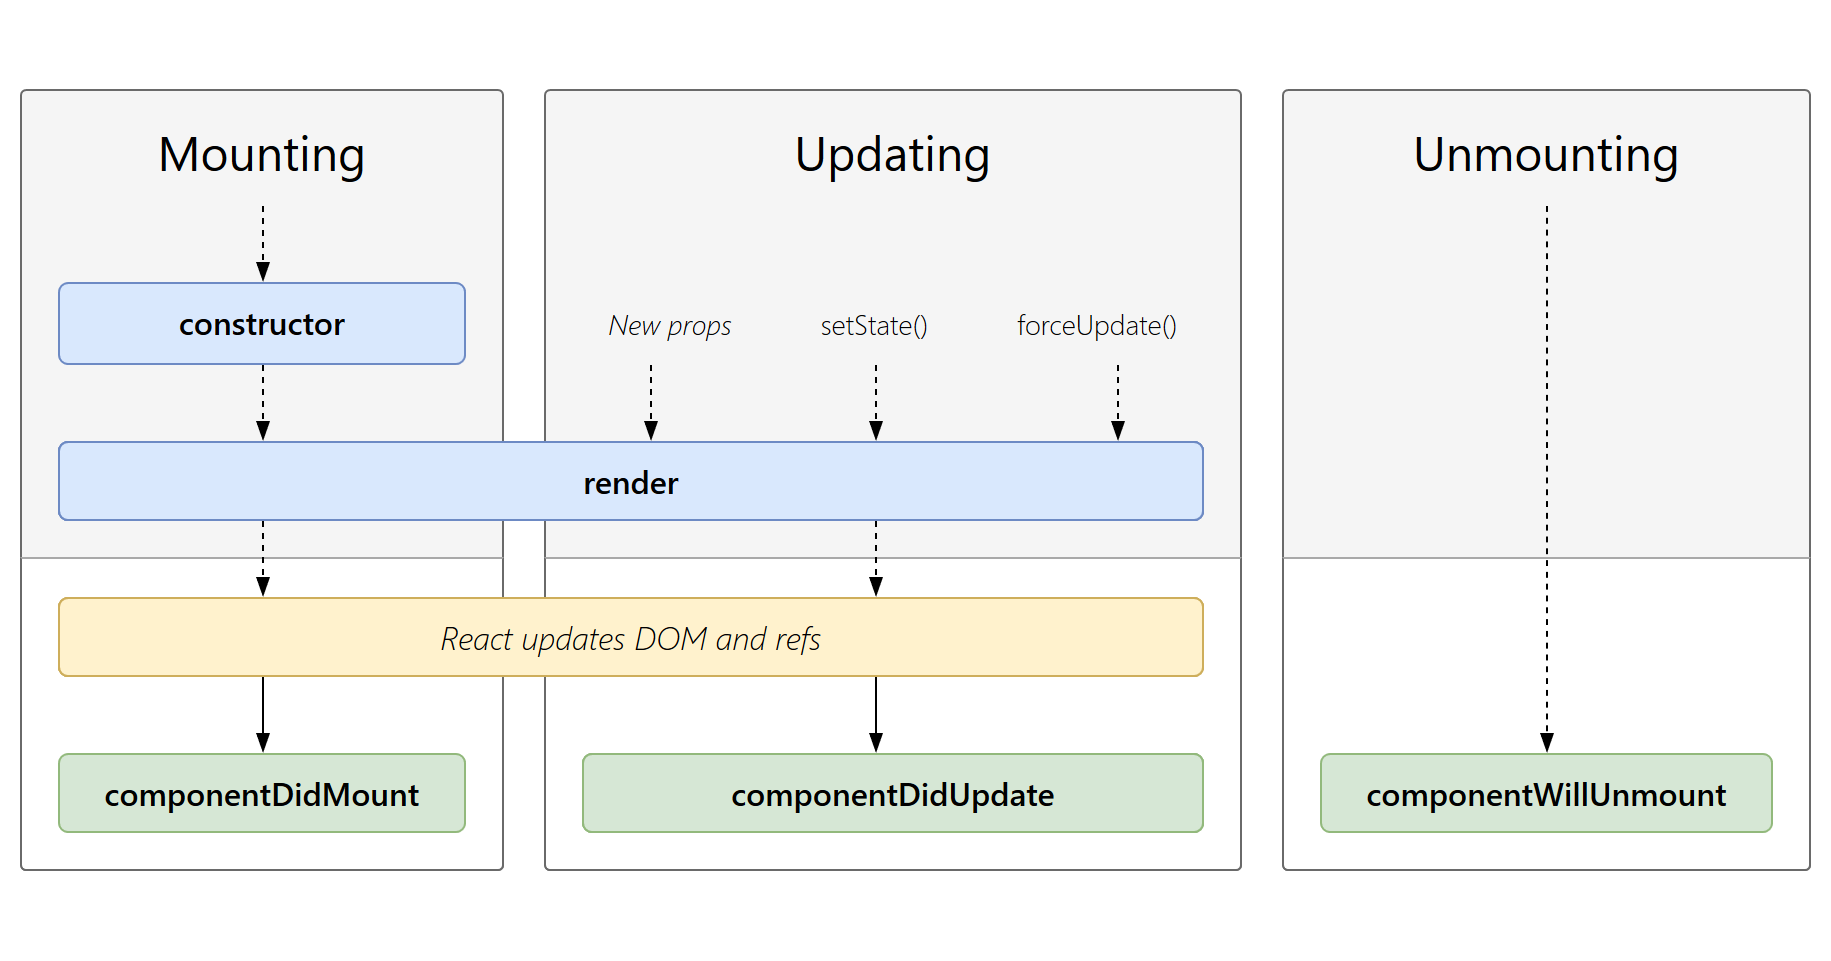
\includegraphics[width=12cm]{figure/literature/react-lifecycle.png}
  % }
  \caption[วัฏจักรการทำงานของ React]{วัฎจักรการ Render, Mount-Unmount และ Update ของ React (React Lifecycle) จาก~\cite{reactcycles}}\label{fig:lit-react}
\end{figure}
\thaijustify{
  React ให้เครื่องมือและโครงสร้างที่สำหรับการสร้างชิ้นส่วนประกอบของส่วนประสานงานผู้ใช้หรือ UI components ได้หลากหลายและมีประสิทธิภาพ~\cite{crockford08js} หนึ่งในข้อได้เปรียบของ React อยู่ที่การใช้ Virtual DOM ที่ช่วยเพิ่มประสิทธิภาพของการ Render องค์ประกอบของ UI และการสร้างแอปพลิเคชันที่มีประสิทธิภาพและสามารถบริหารจัดการ State ของแอปพลิเคชันได้ง่าย~\cite{flanagan20js}
}
\thaijustify{
  ด้วยความนิยมของเครื่องมือตัวนี้ ทำให้ React มีชุมชน (หรือ Community) ที่คอยติดตามและสนับสนุน เป็นเหตุให้เครื่องนี้ถูกนำเขียนใหม่และสร้างเป็น Library หรือ Add-ons อื่น ๆ ที่ทำให้ใช้ React ทำงานและประพฤติในกรอบการทำงานที่ใหญ่ยิ่งขึ้นไปอีก ซึ่งตรงกับเป้าหมายและความคาดหวังที่ทางกลุ่มคณะผู้จัดทำต้องการให้หน้าประสานงานผู้ใช้ (User interface) พึงเป็น
}
\thaijustify{
  หน้าประสานงานผู้ใช้ของซอฟต์แวร์ที่คณะผู้จัดทำกำลังพัฒนานั้นมีกลไกการทำงาน (Function) และการปฏิสัมพันธ์ (Interaction) หมายความว่าถ้าหากบริหารองค์ประกอบของส่วนประสานงานหน้าผู้ใช้หน้าเว็บ (Web UI Component) ได้ไม่ดี จะทำให้อาจกลายเป็นปัญหาและอุปสรรคได้ ดังนั้นเนื่องด้วย React มีระบบการบริหารองค์ประกอบที่สมเหตุสมผลและมีระเบียบระดับหนึ่ง สามารถที่จะเขียนและมององค์ประกอบในเชิงวัตถุหรือ Object-Oriented ได้ดียิ่งขึ้นไปอีก บวกกับการนำ React ด้วยภาษา TypeScript ที่เป็นภาษาเน้น Type และเหมาะกับการเขียนโปรแกรมเชิงวัตถุเป็นอย่างมาก คณะผู้จัดทำจึงได้ตัดสินใจที่จะเลือกใช้เว็บเฟรมเวิร์ค React มาใช้สร้างส่วนประสานงานหน้าเว็บของโครงงานนี้
}
\subsubsection{เฟรมเวิร์ค GoFiber}
\thaijustify{
  GoFiber เป็นเฟรมเวิร์คเบ็ดเสร็จที่เขียนขึ้นมาในภาษา Go (Golang) ที่ใช้สำหรับการพัฒนาเว็บแอปพลิเคชันแบบประสิทธิภาพสูง (High-Performance) พัฒนาขึ้นเพื่อเป็นตัวเลือกที่มีประสิทธิภาพสูงกว่าสำหรับเว็บแอปพลิเคชันที่ใช้งาน Go ทั่วไป โดย GoFiber ถูกออกแบบให้ง่ายต่อการใช้งานและเข้าใจ ด้วยสมรรถนะที่สูงในการดำเนินการต่าง ๆ รวมถึงการทำ Routing และการมี Middleware ต่าง ๆ ทำให้ประสิทธิภาพการทำงานของตัว GoFiber นั้นสูง~\cite{gofiber}
}
\thaijustify{
  จากตัวอย่างสำหรับ Demo ตัว GoFiber ที่ทำโดย \textit{Malomo D.}~\cite{malomo20fiber} เเสดงให้เห็นถึงความสามารถที่โดดเด่นของ GoFiber ได้แก่ความเร็วในการทำงานที่สูง มีการจัดการ Routing ที่มีประสิทธิภาพ นอกจากนี้ GoFiber ยังมีความยืดหยุ่นในการใช้งาน Middleware และการจัดการ HTTP Context ที่เข้าใจง่าย จึงเป็นทางเลือกที่ดีสำหรับการพัฒนาเว็บแอปพลิเคชันที่ต้องการประสิทธิภาพสูงในภาษา Go
}
\thaijustify{
  สมาชิกของกลุ่มคณะผู้จัดทำคุ้นชินกับการใช้ Fiber (ในภาษา JavaScript และ TypeScript) เป็นอย่างดี จึงได้ตัดสินใจนำเอาจะลองนำเอา Fiber ในรูปแบบภาษา Go มาทดลองใช้งานเป็นระบบ API ของโครงงานซอฟต์แวร์
}
\subsubsection{ซอฟต์แวร์ Grafana}
\thaijustify{
  Grafana เป็นเครื่องมือสำหรับการแสดงผลข้อมูลแบบ Real-time และ Monitoring ที่มีความนิยมอย่างแพร่หลายในวงการ IT และพัฒนาซอฟต์แวร์ มันมีความสามารถในการเชื่อมต่อกับแหล่งข้อมูลต่าง ๆ เช่น ฐานข้อมูล, ระบบ Monitor, และ Web Services เพื่อนำข้อมูลมาแสดงผลในรูปแบบกราฟ, ตาราง, และแผนที่เพื่อให้ผู้ใช้งานสามารถวิเคราะห์และทำความเข้าใจข้อมูลได้ง่ายขึ้น~\cite{grafana}
}
\begin{figure}[H]
  \centering
  % \fbox{
  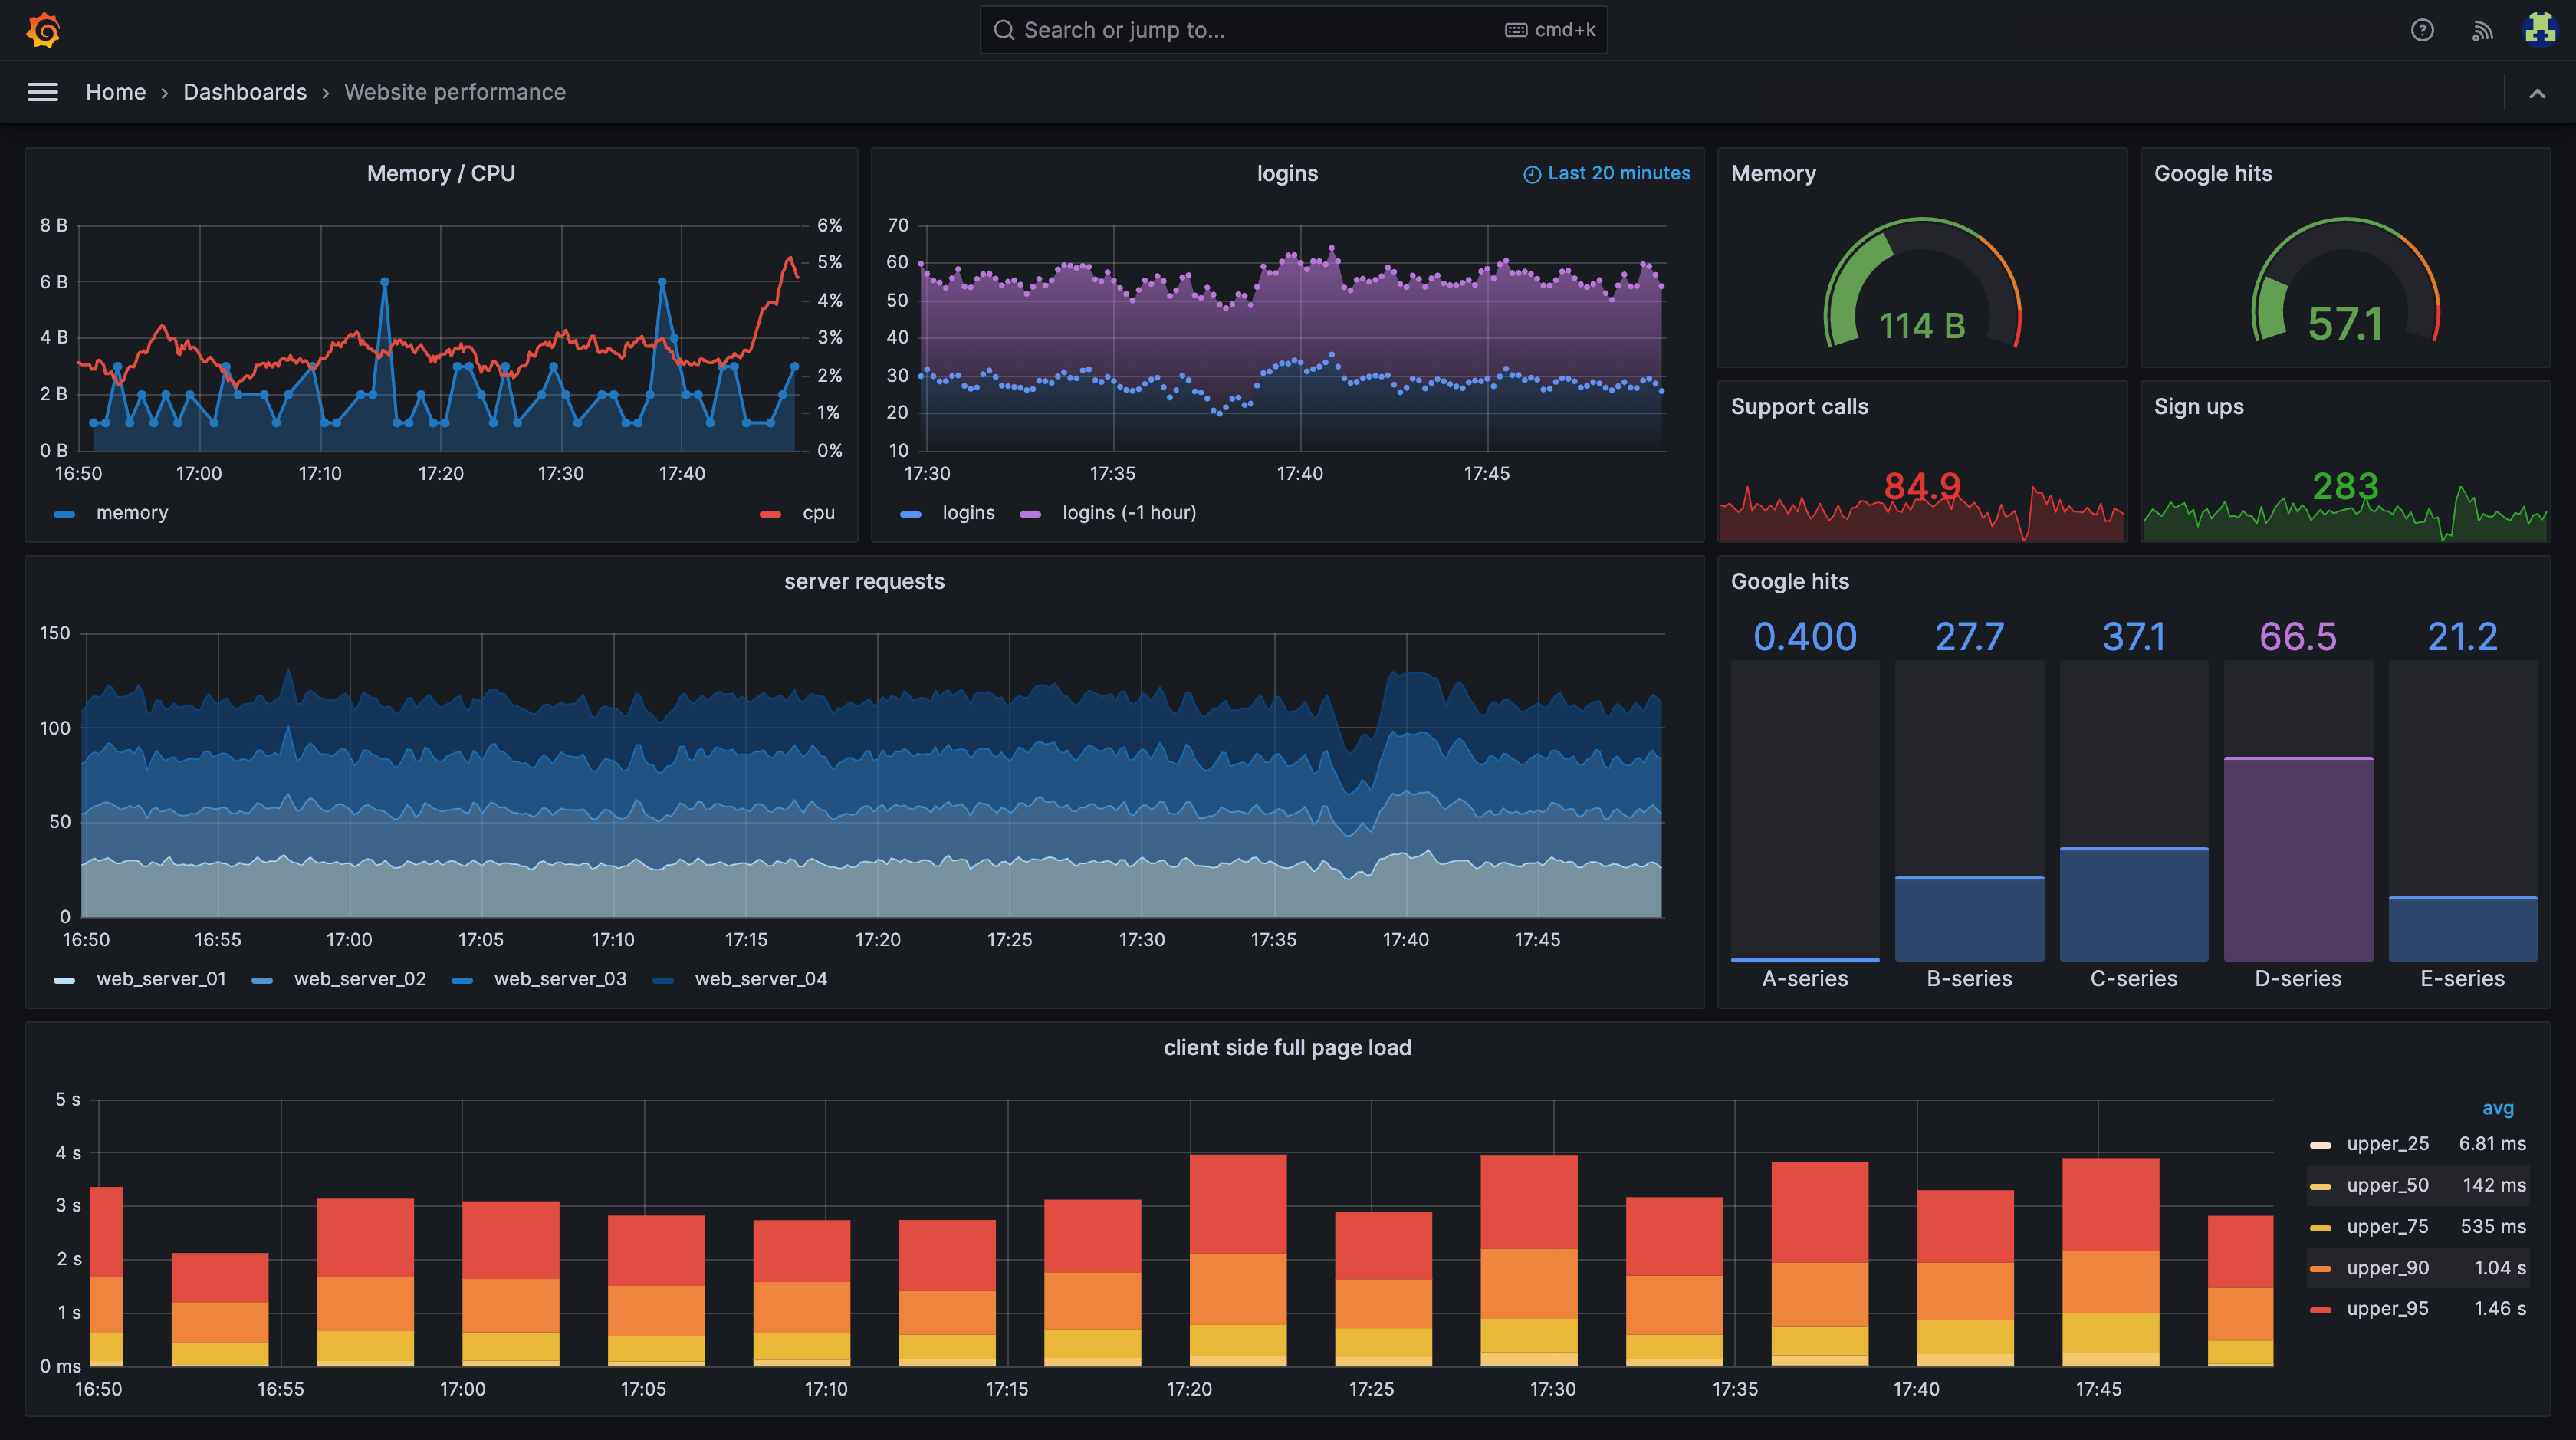
\includegraphics[width=12cm]{figure/literature/grafana.png}
  % }
  \caption[ตัวอย่างหน้าซอฟต์แวร์ Grafana]{ตัวอย่างหน้าซอฟต์แวร์ Grafana จาก~\cite{grafanaoss}}
  \label{fig:lit-grafana}
\end{figure}
\thaijustify{
  Grafana นั้นมีความยืดหยุ่นสูงในการตั้งค่าและการปรับแต่งการแสดงผล สามารถปรับ Dashboard ตามความต้องการของผู้ใช้ได้~\cite{grafana, grafanaoss} จากรายงานของ \textit{Sunil K. \& Savaranan C.}~\cite{sunil21grafana} ถึงแม้ว่าความสามารถในการสร้าง Alert และ Notification จะมีจำกัดและใช้ยาก แต่ Grafana นั้นเต็มไปด้วยฟีเจอร์อื่น ๆ มากมาย ทั้งใช้งานง่ายและมีความยืดหยุ่นสูง มี option ที่สามารถกำหนดเองได้ ทำให้แผงการแสดงภาพที่หลากหลาย ซึ่งทำให้การ Monitor หรือ Visualize ข้อมูล มีสีสันและชีวิตชีวา
}
\thaijustify{
  สมาชิกกลุ่มคณะผู้จัดทำได้มีโอกาสใช้เครื่องมือตัวนี้ตอนฝึกงานกับบริษัทใหญ่แห่งหนึ่งในช่วงปีสาม แล้วมีความเข้าใจและคุ้นเคยกับเครื่องมือตัวนี้เป็นอย่างดี ทางกลุ่มถึงตัดสินใจนำเครื่องมือดังกล่าวมาทดลองใช้กับซอฟต์แวร์โครงการนี้ โดยคาดว่าจะนำเครื่องมือตัวนี้ไปใช้สำหรับเก็บข้อมูลสถิติ เช่น จำนวนคำร้องที่ผู้ใช้ส่งเข้ามา (Requests), ระยะเวลาที่ใช้ในการตอบรับคำขอผู้ใช้ (Response time), จำนวนโปรแกรมภาษาซีที่ได้ตรวจต่อหน่วยเวลา (Total graded assignments per time unit) เป็นต้น
}
\subsubsection{เว็บไซต์ GitHub}
\thaijustify{
  GitHub เป็นเว็บแพลตฟอร์มที่ให้บริการ Hosting ระบบ Version control แบบ Distributed ในรูปแบบของ Git นอกจากนี้, GitHub ยังเป็นสถานที่ที่นักพัฒนาสามารถทำงานร่วมกันและแบ่งปันโค้ดต่าง ๆ ภายใต้รูปแบบของ Repository ทำให้เป็นที่นิยมสำหรับการพัฒนาซอฟต์แวร์ Open Source และโครงการที่มีทีมพัฒนาขนาดใหญ่~\cite{github}
}
\thaijustify{
  GitHub มีความสามารถในการทำงานร่วมกันในโปรเจคผ่าน Git ซึ่งมีข้อได้เปรียบในการจัดการเวอร์ชันของโค้ดและการตรวจสอบการเปลี่ยนแปลง การให้บริการ Issue Tracking และ Pull Request ทำให้งานพัฒนาไปได้อย่างมีระบบและมีความเป็นระบบ~\cite{github, chacon14} แต่ GitHub มีค่าบริการสำหรับการให้บริการ Version Control แด่องค์กรหรือทีมนักพัฒนาที่สูงขึ้นเมื่อเวลาผ่านไป~\cite{githubprice}
}
\thaijustify{
  โครงงานหรือโปรเจคซอฟต์แวร์ส่วนใหญ่ก็นิยมนำ GitHub มาใช้เป็นเครื่องมือทำ Version control แม้แต่โครงงาน~\cite{nattawat20pgs} ก็ใช้ GitHub เช่นกัน บวกกับการที่กลุ่มเรามีคนที่เชี่ยวชาญการใช้ระบบ Version control ของ GitHub แล้ว ทางกลุ่มจึงได้ตัดสินใจนำเลือกใช้เครื่องมือนี้ในงานพัฒนาซอฟต์แวร์นี้
}
\subsubsection{ซอฟต์แวร์ Docker}
\thaijustify{
  Docker เป็นแพลตฟอร์ม Containerization ที่ช่วยให้นักพัฒนาสามารถพัฒนาและใช้งานโปรแกรมได้ง่ายขึ้น โดยไม่ต้องสนใจว่าจะทำงานบนระบบปฏิบัติการ (OS) อะไรทั้งสิ้น~\cite{docker} หลักการของการ Containerization คือการแนบ Dependencies และ Software ทั้งหมดที่ต้องใช้เข้าไปในภาชนะหรือกล่อง ๆ เดียวเป็น Bundle หรือ Container ทำให้สามารถเรียกใช้งานได้ทันที โดยที่ไม่ต้องติดตั้งหรือตั้งค่าเครื่อง ลงโปรแกรมหรือระบบปฏิบัติการเอง~\cite{docker, yıldız23docker} อีกทั้ง Docker มีความสามารถในการทำงานในรูปแบบ Isolation, มีการทำ Resource Optimization, และมีความ Portability ทำให้เป็นเครื่องมือที่ได้รับความนิยมในการพัฒนาและการดำเนินการระบบ~\cite{yıldız23docker}
}
\begin{figure}[H]
  \centering
  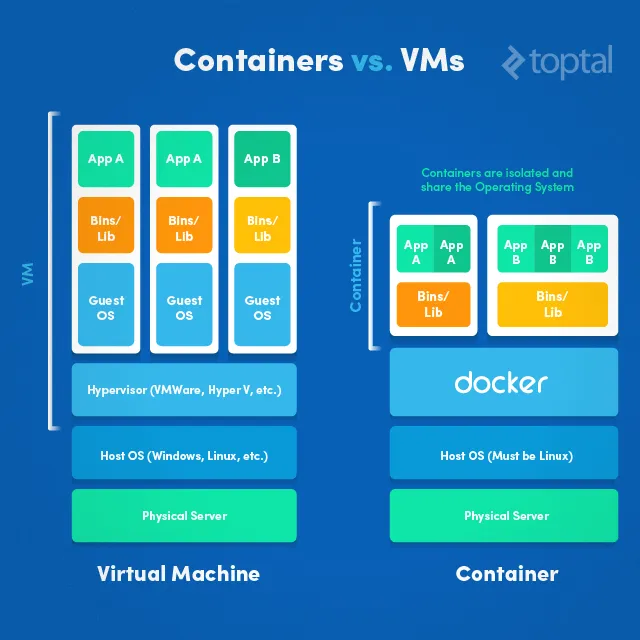
\includegraphics[width=12cm]{figure/literature/docker-compare.png}
  \caption[ภาพเปรียบเทียบเทคโนโลยี Docker กับ Virtual Machine]{การเปรียบเทคโนโลยี Container (Docker) กับเทคโนโลยี Virtual machine (VMWare, Virtual Box, UTM เป็นต้น) ภาพจาก~\cite{dockerdummies}}\label{fig:lit-docker}
\end{figure}
\thaijustify{
  Docker ช่วยลดปัญหาที่เกิดขึ้นจากความแตกต่างของระบบปฏิบัติการและสภาพแวดล้อมการทำงานระหว่าง Development และ Production โดยลดปัญหา \textit{It works on my machine!} ซึ่งก็คือปัญหาที่โปรแกรมจะทำงานในเครื่องคอมพิวเตอร์เครื่องหนึ่งแต่ไม่ทำงานในอีกเครื่องหนึ่ง~\cite{yıldız23docker} จากบทความของ \textit{Chesterwood R.}~\cite{chesterwood21microservice} Docker ยังช่วยในการปรับใช้โปรแกรมในลักษณะ Microservices Architecture ทำให้การพัฒนาและการดูแลรักษาระบบเป็นไปอย่างมีประสิทธิภาพ
}
\thaijustify{
  เช่นเดียวกับเครื่องมือก่อน ๆ Docker อาจมีความซับซ้อนสูงขึ้นและเรียนรู้การใช้งานยาก ในการกำหนดค่าและจัดการ Container หลาย ๆ ตัวพร้อมกันในระบบก็๋เป็นเรื่องที่ยากและใช้ความรู้มหาศาล~\cite{dockerdoc} และจากความเห็นของ \textit{Yıldız H.}~\cite{yıldız23docker} ถึงเเม้ Docker จะเป็นซอฟต์แวร์ที่ Light-weighted ในบางกรณี Docker อาจส่งผลกระทบต่อการทำงานโดยภาพรวมของระบบ System Performance หากบริหารไม่ดี
}
\subsubsection{ซอฟต์แวร์ Terraform}
\thaijustify{
  Terraform เป็นเครื่องมือสำหรับ Infrastructure as Code (IaC) ที่ออกแบบมาเพื่อจัดการและกำหนดค่า Infrastructure ทั้งใน Cloud และ On-Premises อย่างมีประสิทธิภาพ~\cite{terraform} ผู้ใช้สามารถใช้ภาษาที่อ่านง่ายเพื่อกำหนดค่าและสร้าง Infrastructure ที่ต้องการ เช่น Virtual Machines, Networks, Databases และ Resources อื่น ๆ ในรูปแบบของ Code~\cite{terraform} จากบทความเรื่องข้อดีของ Terraform โดย \textit{Tripathi P.}~\cite{tripathi23terraform} ได้พูดถึงข้อดีสำคัญของ Terraform หลายประการตั้งแต่ความยืดหยุ่น, ทนทาน, ไปจนถึงความสามารถในทำงานร่วมกับหลาย Cloud Provider อย่างมีประสิทธิภาพ
}
\thaijustify{
  การใช้ Terraform ช่วยลดการพิมพ์ Configuration Code ที่จะใช้กำหนดค่า Infrastructure ลงไปใน Code ของโปรเจคและช่วยในการตรวจสอบสถานะและการดำเนินการ Infrastructure อย่างทันที แต่ผู้ใช้ต้องเรียนรู้และทำความเข้าใจการใช้งาน Terraform อย่างลึกซึ้งเพื่อให้การใช้งานมีประสิทธิภาพ~\cite{stanfield22iac}
}
\subsubsection{ซอฟต์แวร์ Kubernetes}
\thaijustify{
  Kubernetes เป็นซอฟต์แวร์ประเภท Orchestrator ที่ใช้ในการจัดการและควบคุม Containers ในรูปแบบ Cluster มีความสามารถในการปรับขยายและจัดการสถานะของ Containers ต่าง ๆ ในทันที ทำให้เป็นเครื่องมือที่ดีสำหรับการปรับใช้และการจัดการ Microservices และ Applications ที่ทำงานบน Containers อีกทั้ง Kubernetes ช่วยลดภาระในการสร้าง, ดูแล, และปรับขยายระบบที่มีมากถึงหลายหลาย Containers~\cite{kubernetes}
}
\thaijustify{
  นักพัฒนาซอฟต์แวร์ส่วนใหญ่ เล็งเห็นผลประโยชน์ของการนำ Kubernetes มาใช้ในเข้าเข้าขั้นตอนการนำซอฟต์แวร์ลงเปิดใช้งานบนเซิร์ฟเวอร์ (หรือการ Deploy) เพราะความสามารถในการ การทยอยเปลี่ยน Image version หรือเรียกว่าการ Rollout เพื่อหลีกเลี่ยงการเกิด Downtime ระหว่างการเปลี่ยนซอฟต์แวร์ให้เป็นเวอร์ชั้นใหม่~\cite{kubemed20}
}
\thaijustify{
  ความสามารถในการตรวจจับและแก้ไขข้อผิดพลาดในการทำงานของ Containers รวมถึงการปรับเปลี่ยนอัตโนมัติหรือเริ่มต้นการทำงานใหม่เอง (Automatic) ในกรณีที่มี Containers ล่ม ทำให้ระบบยืดหยุ่นและทนทานมากขึ้น~\cite{kubernetes} แต่เช่นเดียวกับตัว Docker เอง การจัดการ Kubernetes อาจมีความซับซ้อนและต้องการเรียนรู้การใช้งานในระดับที่สูง
}
\subsubsection{ซอฟต์แวร์บริหารฐานข้อมูล MySQL}
% TODO: Add more citation for MySQL
\thaijustify{
  ซอฟต์แวร์ MySQL เป็นระบบจัดการฐานข้อมูลแบบ Relational Database Management System (RDBMS) ที่เป็น Open Source และได้รับความนิยมอย่างแพร่หลาย มีความสามารถในการจัดเก็บและจัดการข้อมูลในรูปแบบตารางที่สอดคล้องกับโครงสร้างของฐานข้อมูล~\cite{mysql} ทำให้เป็นทางเลือกที่ดีสำหรับโปรเจคที่มีโครงสร้างข้อมูลที่แน่นอน เนื่องด้วยความเป็นที่นิยมและการที่ยังมีคนใช้ประโยชน์จากตัวซอฟต์แวร์ตัสนี้อยู่ MySQL มี Community Edition ที่ให้บริการฟรีและมีการพัฒนาที่อย่างต่อเนื่อง~\cite{mysqlcomm}
}
\thaijustify{
  ข้อดีของ MySQL รวมถึงประสิทธิภาพในการค้นหาและดึงข้อมูล, รองรับการใช้งานที่หนักหน่วง, และมีความปลอดภัยในการจัดการข้อมูล แต่ก็ใช่ว่า MySQL จะเหมาะสมกับทุกโปรเตค  บางครั้ง MySQL อาจจะไม่เหมาะสมกับโปรเจคที่มีความซับซ้อนและต้องการการจัดการข้อมูลในมิติที่หลากหลาย
}
\subsubsection{ซอฟต์แวร์บริหารฐานข้อมูล InfluxDB}
\thaijustify{
  ระบบซอฟต์แวร์ InfluxDB เป็นระบบจัดการฐานข้อมูลแบบ Time Series ที่ออกแบบมาเพื่อจัดเก็บและจัดการข้อมูลที่มีการเปลี่ยนแปลงตลอดเวลา นิยมถูกใช้ในงานที่ต้องการจัดเก็บข้อมูลการวัดหรือเวลาจริง เช่น ข้อมูลเซ็นเซอร์ หรือข้อมูลการทดสอบและข้อมูลการวิเคราะห์จากต้นทางที่ส่งมาพร้อมเวลา timestamp~\cite{influxdb} มีความยืดหยุ่นและสามารถทำงานร่วมกับหลายแพลตฟอร์ม~\cite{influxdb-platforms}
}
\thaijustify{
  มันมีความเป็นเลิศในด้านประสิทธิภาพของทรัพยากร ทำให้มีฟังก์ชันการทำงานที่สำคัญโดยใช้ทรัพยากรน้อยที่สุด ความสามารถในการรวบรวมข้อมูลอนุกรมเวลาใน Bucket รายชั่วโมงและรายวันได้อย่างมีประสิทธิภาพ ช่วยให้การสืบค้นและการวิเคราะห์ข้อมูลง่ายขึ้น นอกจากนี้ความยืดหยุ่นของนโยบายการเก็บรักษายังช่วยให้สามารถปรับระยะเวลาการเก็บรักษาข้อมูลได้อย่างง่ายดาย ป้องกันการล่มเนื่องจากพื้นที่ไม่เพียงพอเก็บข้อมูล~\cite{sandholm17influx}
}
\thaijustify{
  อย่างไรก็ตาม หากออกแบบไม่ดี ก็สามารถนำไปสู่ปัญหาด้านประสิทธิภาพได้ โดยเฉพาะอย่างยิ่งกับการกำหนดค่าเริ่มต้นที่สร้างส่วนแบ่งข้อมูลใหม่ทุกสัปดาห์และเก็บข้อมูลไว้อย่างไม่มีกำหนดหรือ การปรับสมดุลขนาดของชิ้นส่วนข้อมูล (Shard) เพื่อเพิ่มประสิทธิภาพเวลาในการเขียนและคิวรีอาจเป็นเรื่องที่ท้าทายและต้องพิจารณาอย่างรอบคอบ นอกจากนี้การพึ่งพาระหว่างการกำหนดค่าส่วนแบ่งข้อมูลและระยะเวลาการเก็บรักษายังมีความเสี่ยงที่ข้อมูลจะสูญหายหากไม่ได้รับการจัดการอย่างเหมาะสม โดยเฉพาะอย่างยิ่งเมื่อมีการใช้ส่วนแบ่งข้อมูลขนาดใหญ่ควบคู่ไปกับระยะเวลาการเก็บรักษาที่สั้น~\cite{sandholm17influx}
}
\subsubsection{ซอฟต์แวร์ Prometheus}
% TODO: Add more citation for Prometheus
\thaijustify{
  Prometheus เป็นระบบการตรวจสอบและติดตาม (Monitoring and alerting) ที่ถูกออกแบบมาสำหรับระบบที่มีโครงสร้างที่ยืดหยุ่นและต้องการการดูแลที่ส่วนตัว~\cite{prometheus} มีความสามารถในการเก็บข้อมูลและวิเคราะห์ข้อมูลเพื่อตรวจสอบปัญหาและเป็นเครื่องมือที่มีประสิทธิภาพในการจัดการระบบที่ใหญ่ ตัวซอฟตแวร์ มีการส่งเสริมการใช้งานร่วมกับ Kubernetes และมีการส่งเสริมที่ดีในการใช้งานที่แพร่หลายในระบบคลาวด์
}
\thaijustify{
  ความยืดหยุ่นและการติดตามเหตุการณ์ในเวลาที่เป็นเรียลไทม์เป็นจุดเด่นสำคัญของ Prometheus, ทำให้เป็นเครื่องมือที่เหมาะสมสำหรับการค้นหาและแก้ไขปัญหาที่เกิดขึ้นทันที แต่ในระบบที่มีขนาดใหญ่และต้องการการเก็บข้อมูลที่ยาวนาน แต่พื้นที่เก็บข้อมูลของ Prometheus อาจมีความจำกัดและข้อมูลอาจล้นเกินได้
}
\subsubsection{ซอฟต์แวร์ RabbitMQ}
\thaijustify{
  RabbitMQ เป็นระบบ Message Broker ที่มีคุณสมบัติและบริการในการจัดการและส่งข้อมูลระหว่างแอปพลิเคชันต่าง ๆ~\cite{rabbitmq} ในรูปแบบที่มีประสิทธิภาพ ด้วยความที่ซอฟต์แวร์เป็น Open Source ทำให้ได้รับความนิยมเป็นอย่างสูง ได้ถูกนำมาใช้การทำงานในสภาพแวดล้อมที่ต้องการการกระจายข้อมูลและการคอมมูนิเคชัน อีกทั้งการใช้ RabbitMQ ช่วยลดความซับซ้อนในการสื่อสารระหว่างบริการและแอปพลิเคชัน, ทำให้ระบบสามารถทำงานได้อย่างยืดหยุ่นและมีประสิทธิภาพ~\cite{rabbitmq}
}
% TODO: Validate following paragraph's citation
\thaijustify{
  ความยืดหยุ่นของ RabbitMQ ทำให้เป็นเครื่องมือที่มีประสิทธิภาพสำหรับการทำ Message Queue และการจัดการกับการแลกเปลี่ยนข้อมูลที่ต้องการการทำงานแบบอนุกรม~\cite{roy17rabbitmq} ในเเง่ของข้อเสียการดูแลรักษาและบริหารจัดการ RabbitMQ ในสภาพแวดล้อมที่มีใช้งานการสื่อสารมาก ๆ อาจมีความซับซ้อน~\cite{hanwell17rabbitmq}
}
\subsubsection{ซอฟต์แวร์ Argo CD}
\thaijustify{
  Argo CD เป็นเครื่องมือทำ Continuous Deliveries ของ GitOps ซึ่งออกแบบมาโดยเฉพาะสำหรับใช้กับระบบ Kubernetes ทำให้การปรับใช้แอปพลิเคชันและการกำหนดค่ากับคลัสเตอร์ Kubernetes เป็นแบบไปอย่างง่ายดายโดยอัตโนมัติ ด้วยการใช้ประโยชน์จาก Git เป็นแหล่งที่มาของข้อมูลลับ (Secret Variables) สำหรับการเข้าระบบผ่านระบบ Authentication เพื่อเข้าไปตั้งค่าแอปพลิเคชัน Kubernetes ทำให้ Argo CD เปิดใช้งานเวิร์กโฟลว์ GitOps โดยที่การเปลี่ยนแปลงที่ทำกับพื้นที่เก็บข้อมูล Git จะทริกเกอร์การปรับใช้แอปพลิเคชันโดยอัตโนมัติ~\cite{argodoc}
}
\thaijustify{
  ข้อดีที่สำคัญประการหนึ่งของการใช้ Argo CD คือความสามารถในการจัดเตรียมแนวทางการควบคุมเวอร์ชันสำหรับควบคุม จัดการและบริหารแอปพลิเคชัน Kubernetes ด้วยการจัดเก็บการกำหนดค่าแอปพลิเคชันไว้ในที่เก็บ Git ทีมดูแลซอฟต์แวร์สามารถติดตามการเปลี่ยนแปลง ทำงานร่วมกันอย่างมีประสิทธิภาพและสามารถย้อนกลับเป็นเวอร์ชันก่อนหน้าได้อย่างง่ายดายหากเกิดข้อผิดพลาด วิธีการแบบรวมศูนย์นี้ช่วยเพิ่มการมองเห็นและการควบคุมกระบวนการปรับใช้ ลดความเสี่ยงของการกำหนดค่าที่ลอยไปและรับประกันว่าสภาพแวดล้อมทั้งหมดคงการทำงานตรงกัน (Synchronized) ~\cite{argodocsync}
}
% TODO: Summary Writing of Chapter 2
\section{สรุปการศึกษาค้นคว้า}
\thaijustify{
  จากที่ได้กล่าวและอธิบายมาทั้งหมด คณะผู้จัดทำได้คาดหวังและวางแผนที่จะเอาทฤษฎี หลักการ วิทยาการและเทคโนโลยีทั้งหมดที่ได้ศึกษามา นำไปประยุกต์ใช้ประโยชน์ในขั้นตอนการออกแบบและสร้างระบบซอฟต์แวร์ของโครงการต่อ ๆ ไป โดยจะสรุปและบรรยายว่าส่วนเนื้อหาแต่ละส่วนที่ได้เขียนไว้ในบทนี้ คาดว่าจะประยุกต์ใช้งานหรือเป็นแหล่งอ้างอิงให้กับส่วนไหนของโครงการได้บ้าง
}
\subsection{การประยุกต์ใช้ทฤษฎีและหลักการ}
\thaijustify{
  หลักการเขียนโปรแกรมเชิงวัตถุหรือ OOPs จาก~\cite{booch87, meyer2000, apollo22oop} เป็นหลักการเขียนโปรแกรมที่มีประโยชน์อย่างมาก สามารถที่จะทำให้ผู้พัฒนาซอฟต์สามารถที่จะออกแบบและสร้างที่มีความต้องการและมีการทำงานขึ้นมาได้อย่างง่ายได้ หากใช้ร่วมกับแนวคิดการออกแบบแยกข้อกังวลและแยกความรับผิดชอบหรือ SoC นั้น จะทำให้ระบบซอฟต์แวร์มีส่วนการทำงานที่ถูกนิยามและวางไว้อย่างชัดเจน มีหน้าถ้าหากส่วนใดเกิดปัญหาขึ้นมาในส่วนใดของซอฟต์แวร์ ก็จะสามารถที่จะสืบหาที่มาของปัญหาได้อย่างรวดเร็วเพราะผู้พัฒนาก็จะรู้ว่าส่วนใดในซอฟต์แวร์ที่รับผิดชอบหน้าที่นั้น ๆ~\cite{nattawat20pgs, wikipedia04soc}
}
\thaijustify{
  แต่จากที่ได้ศึกษาจาก~\cite{thomas99pragmatic, fowler13oop, nattawat20pgs} ถ้าหากใช้หลักการเขียนโปรแกรมเชิงวัตถุมากเกินควรจำเป็น ก็ย่อมทำให้เกิดผลเสียได้ อย่างซอฟต์แวร์ที่เขียนขึ้นมามีความซับซ้อนมากไป มีขั้นตอนในการแก้ปัญหาใดปัญหาหนึ่งที่ยุ่งยากหลายขั้นตอน วัตถุหนึ่งต้องส่งข้อมูลชุดหนึ่งไปแก้ในวัตถุชุดต่อ ๆ ไป ทำให้การแก้ปัญหาง่าย ๆ กลายเป็นเรื่องยากหรือเรียกว่าเป็นการแก้ปัญหาที่~\textit{Over-engineered} มาก เห็นได้อย่างชัดเจนจากการศึกษาและวิเคราะห์ระบบของ~\cite{nattawat20pgs}
}
\thaijustify{
  ในเมื่อกลุ่มเราได้ตัดสินใจนำหลักการเขียนเชิงวัตถุมาใช้ ทางกลุ่มเราเห็นควรว่าควรนำการออกแบบของการเขียนโปรแกรมเชิงวัตถุรูปแบบหนึ่งหรือ Design Pattern มาใช้ในการออกแบบโครงสร้างระบบ โดยเราได้ศึกษารูปแบบการส่งต่อ Dependencies (หรือ Dependencies Injection)~\cite{shore06, fowlerDI, freeman09} เพราะเล็งเห็นว่าการใช้รูปแบบนี้จะทำให้กลุ่มเรา สามารถที่บริหารจัดการความสัมพันธ์และการพึ่งพากันระหว่างโมดูลได้ และทำให้องค์ประกอบของระบบยิ่งแยกหน้าที่กันออกไปอีก ทําให้กลุ่มเรานั้นสามารแยกส่วนประกอบออกมาแยกทดสอบได้~\cite{fowlerDI, tiwaristackdi, toanstackdi}
}
\subsection{การประยุกต์ใช้เครื่องมือและเทคโนโลยี}
\thaijustify{
  หลังจากที่ได้ค้นคว้าหลักการในการออกแบบ ทางกลุ่มก็ได้ไปศึกษาและนั่งคัดกรองหาเครื่องมือที่คิดว่าน่าจะเหมาะสมมาใช้กับโครงงานซอฟต์แวร์นี้ โดยกลุ่มเราเริ่มจากการสรรหาเครื่องมือและเทคโนโลยีที่จะเป็นแกนกลางสำคัญที่จะทำให้โครงสร้างซอฟต์แวร์มั่นคง จากการได้ไปดูโครงการ~\cite{nattawat20pgs} ซึ่งเป็นโครงการที่ทำซอฟต์แวร์ที่มีวัตถุประสงค์มุ่งหมายเดียวกัน โครงการดังกล่าวได้นำ Docker และ Kubernetes ซึ่งเป็นเทคโนโลยีการบริหารโครงสร้างซอฟต์แวร์ที่ทันสมัยมาใช้จัดการบริหารระบบซอฟต์แวร์
}
\thaijustify{
  การใช้ Docker ก็เป็นสิ่งที่น่าสนใจ หลังจากได้ศึกษา~\cite{docker, yıldız23docker, dockerdummies, chesterwood21microservice, dockerdoc} การใช้ Docker นั้นจะทำให้กลุ่มเรามองซอฟต์แวร์ระบบแต่ละองค์ประกอบแยกกันเป็นอิสระต่อกันมากขึ้น จะสามารถทำให้กลุ่มเราทำงานและพัฒนาซอฟต์แวร์ง่ายขึ้น เมื่อเกิดปํญหาส่วนไหนก็จะสามารถสืบหาสาเหตุได้ คล้ายกับหลักการ OOPs ที่ได้กล่าวมาในหัวข้อที่แล้ว อีกทั้งการมองเป็น Container นั้นจะทำให้ การจัดการบริหารกับการเปิด-ปิดซอฟต์แวร์สะดวกยิ่งขึ้น กลุ่มเราสามารถที่จะยกซอฟต์แวร์ทั้ง Container ไปวางติดตั้งที่ไหนก็ได้ เพราะแนบ Environment ไปกับ Container ด้วย จึงจะเปิดบนระบบปฏิบัติการไหนก็ได้ ทั้งเพื่อพัฒนาโปรแกรมกันเอง (Development) หรือเพื่อติดตั้งเพื่อเปิดบริการ (Production) ก็ตาม
}
\thaijustify{
  ในส่วนของ Kubernetes~\cite{kubernetes, kubemed20} แม้ว่าจะน่าสนใจที่จะนำมาใช้ ทางกลุ่มของเราคิดว่าปัญหาที่โครงการนี้ถูกตั้งขึ้นมาเพื่อจะแก้ไขนั้น ไม่ได้มีความยุ่งยากมากพอที่จำเป็นต้องสร้างระบบโครงสร้างซอฟต์แวร์ ที่ถูกสนับสนุนด้วย Kubernetes ทางกลุ่มเกรงว่ามันจะเป็นการ \textit{Over-engineer} เกินไป แทนที่ซอฟต์แวร์จะใช้วิธีง่ายในการแก้ปัญหาง่าย ๆ อย่างแค่การส่งโปรแกรมขึ้นไปให้ตรวจและรับผลกลับมา แต่ถ้าหากใช้วิธียาก ๆ ด้วยระบบโครงสร้างที่ยาก จะทำให้ซอฟต์แวร์ทำงานช้าและมีประสิทธิภาพการทำงานที่แย่ลง ซึ่งเกิดขึ้นในโครงงาน~\cite{nattawat20pgs}
}
\thaijustify{
  สำหรับเขียนส่วนประสานงานผู้ใช้หรือ User Interface หน้าเว็บไซต์ กลุ่มเราเห็นว่าจะใช้ React ที่เขียนด้วย TypeScript เพราะจาก~\cite{flanagan20js, crockford08js, hejlsbergts, microsoftts, cherny19ts} React ช่วยให้การสร้างและจัดการ UI Components เป็นไปอย่างรวดเร็วและยืดหยุ่น ขณะที่ TypeScript เพิ่มความปลอดภัยในการเขียนโค้ดด้วยการตรวจสอบชนิดข้อมูล (Type Checking) ช่วยลดข้อผิดพลาดที่อาจเกิดขึ้นในระหว่างการพัฒนา อีกทั้งการใช้ TypeScript นั้นจะทำให้เราสามารถมององค์ประกอบเว็บเป็นวัตถุได้ สามารถใช้หลักการ OOPs~\cite{apollo22oop, moses22obj, johnson88classobj, sakpal18inheritance, stroustrup94inheritance, javapolymorph, nzeruekenneth23polymorph, ntu20polymorph, saladpukabstract, liskov87abstaction, raut22encapsule, nishad22encapsulation} ที่เคยได้ศึกษามาได้ และการมองและใช้ให้องค์ประกอบหน้าประสานงานเป็นวัตถุชิ้นหนึ่ง ทำให้เราสามารถที่จะนำวัตถุหรือองค์ประกอบหน้าเว็บอันใดก็ได้ นำกลับมาใช้ใหม่ได้ง่าย ลดความซับซ้อนในการพัฒนาและบำรุงรักษา
}
\thaijustify{
  สำหรับส่วนของระบบซอฟต์แวร์ในหลังบ้านหรือ Backend System กลุ่มคณะผู้จัดทำใช้การไลบารีหรือเฟรมเวิร์คสำหรับบริหารคำขอหรือ Application Interface (API) Server เป็น Fiber ที่เขียนด้วยภาษา Go เพราะทางกลุ่มเราคิดเห็นว่า การใช้เครื่องมือทั้งสองอย่างอาจทำให้ประสิทธิภาพการทำงานที่สูงและรองรับการเชื่อมต่อหลายตัวพร้อมกัน เพราะ Fiber เป็นเว็บเฟรมเวิร์คที่เบาและมีประสิทธิภาพสูง ซึ่งเหมาะสมกับการพัฒนา API Server ที่ต้องรองรับคำขอหลายตัวพร้อมกันได้ดี~\cite{gofiber, malomo20fiber} ส่วนภาษา Go เองมีความสามารถในการจัดการกับความขนาน (Concurrency) ได้อย่างยอดเยี่ยม บวกกับความง่ายในการติดตั้งและบริหารจัดการซอฟต์แวร์ เพราะ Go เป็นภาษาที่คอมไพล์เป็นไบนารีขนาดเล็กและไม่ต้องการการพึ่งพาเพิ่มเติม ทำให้การ deploy ซอฟต์แวร์ที่เขียนด้วย Go เป็นไปอย่างง่ายดายและรวดเร็ว ถูกออกแบบมาให้มีความเสถียรและมีการบริหารจัดการหน่วยความจำที่ดี ช่วยลดข้อผิดพลาดที่เกิดจากการจัดการหน่วยความจำในโปรแกรม อีกทั้งยังมีเครื่องมือที่ช่วยในการทดสอบและตรวจสอบความปลอดภัยของโค้ด~\cite{pike12go, donovan15go, pike12godev, golangorg}
}
\thaijustify{
  ส่วนเครื่องมือที่เหลืออื่น ๆ ได้แก่ฐานข้อมูล MySQL~\cite{mysql, mysqlcomm} และ InfluxDB~\cite{influxdb, influxdb-platforms, sandholm17influx}, ซอฟต์แวร์สำหรับวิเคราะห์สภาพระบบและเก็บ Metrics อย่าง Grafana~\cite{grafana, grafanaoss, sunil21grafana} กับ Prometheus~\cite{prometheus}, ซอฟต์แวร์บริหารจัดการคิว RabbitMQ~\cite{rabbitmq, roy17rabbitmq, hanwell17rabbitmq}, ซอฟต์แวร์สำหรับริหารซอร์สโค้ด จัดส่งและอัพเดตระบบซอฟต์แวร์อย่าง GitHub~\cite{github, githubprice,chacon14} กับ Argo~\cite{argodoc, argodocsync} เป็นต้น เป็นเพียงเครื่องมือเสริมหรือสนับสนุนการทำงานของระบบที่สมาชิกในกลุ่มเคยได้ใช้กับโครงการซอฟต์แวร์ที่เคยได้ทำในอดีต เครื่องมือต่าง ๆ เหล่านั้น ทางกลุ่มเราคาดว่าจะนำมาใช้เสริมการทำงานของซอฟต์แวร์โครงการนี้ เพื่อที่จะทำให้ซอฟต์แวร์โครงการนี้ทำงานได้ดียิ่งขึ้นไปอีกหรือไม่ก็ทำให้กลุ่มเราสามารถที่จะทำงานกับซอฟต์แวร์โครงการได้สะดวกยิ่งขึ้นไปอีก
}
\pagebreak
%%%%%%%%%%%%%%%%% Design and Methodologies %%%%%%%%%%%%%%%%%%%%%
\chapter{วิธีการดำเนินงาน}

\thaijustify{
  ในบทที่ 3 จะกล่าวถึงภาพรวมของซอฟต์แวร์ของโครงงาน โครงสร้างระบบที่ทางคณะผู้จัดทำโครงการได้วางเอาไว้ ลักษณะฐานข้อมูลที่ใช้ในการจัดเก็บข้อมูล การใช้งานระหว่างระบบออกแบบมาตอบโจทย์ผู้ใช้งาน รวมไปถึงการบริหารงานภายในระบบ ซึ่งถูกออกแบบไว้อย่างดีโดยได้นำเอาเครื่องมือและแนวคิดที่ได้ศึกษาค้นคว้ามาในบทก่อนหน้ามาประยุกต์ มาใช้สร้างและออกแบบสถาปัตยกรรมระบบที่มีความเป็นระเบียบและเหมาะสม ระบบฐานข้อมูลที่เรียบง่าย ด้วยการใช้เครื่องมือและเทคโนโลยีที่เหมาะสมและทันสมัยที่ได้ค้นคว้ามา โดยคาดหวังว่าระบบซอฟต์แวร์ดังกล่าวจะสามารถทำงานอย่างมีประสิทธิภาพ ประมวลผลเร็วและทนทานต่อข้อผิดพลาด
}
\section{รายละเอียดของโครงงาน}
\thaijustify{
  ในหัวข้อแรกของบทที่ 3 คณะผู้จัดทำได้นำข้อมูลและองค์ความเข้าใจที่ได้จากการไปสัมภาษณ์และสอบถามจากผู้ใช้หลาย ๆ คน มากลั่นกรองและสรุปเป็นข้อกำหนดที่ซอฟต์แวร์โครงการนี้จำเป็นต้องมีเพื่อบรรลุเป้าหมายของโครงการ พร้อมทั้งแยกผู้ใช้ประเภทใดบ้างและแต่ละประเภทสามารถเข้าถึงข้อกำหนดหรือข้อใช้งานข้อไหนบ้าง ทั้งหมดที่ได้กล่าวมานั้นจะถูกสรุปเป็นตารางข้อกำหนดและแผนผังกรณีใช้งานในหัวข้อนี้
}
\subsection{ข้อกำหนดและความต้องการของระบบ}
\thaijustify{
  ในส่วนนี้ จะกล่าวถึงข้อกำหนดของซอฟต์แวร์หรือ User Requirements ซึ่งประกอบด้วยการทำงานในส่วนต่าง ๆ แยกประเภทเป็นตามหมวดหมู่ผู้ใช้ดังนี้ เจ้าของระบบหรือผู้ดูแลระบบ (Admin), เจ้าของห้องเรียน เจ้าของกลุ่มเรียนหรืออาจารย์ผู้สอน (Owner), ผู้ช่วยเจ้าของห้องหรือผู้ช่วยสอน (Moderator), นักศึกษา (Student), ผู้เข้าร่วมกิจกรรมหรือการแข่งขันฯ (Attendee), ผู้ใช้ทั่วไป (Registered User) และบุคคลทั่วไปหรือบุคคลภายนอก (Guest User)
}
%%%%%%%%%%% SOFTWARE REQUIREMENT TABLE %%%%%%%%%%%
\begin{longtable}{p{3cm}|ccccccc}
  % First header
  \caption{ข้อกำหนดของซอฟต์แวร์}\label{tbl:soft-req1}                                                                                                 \\ % First caption
  \hline\hline
  Feature                                         & Guest User & Registered User & Student    & Attendee   & Moderator  & Owner      & Admin      \\
  \hline\hline
  \endfirsthead
  % Re-occurring header
  \caption[]{ข้อกำหนดของซอฟต์แวร์ (ต่อ)}                                                                                                               \\ % Cont. caption
  \hline\hline
  Feature                                         & Guest User & Registered User & Student    & Attendee   & Moderator  & Owner      & Admin      \\
  \hline\hline
  \endhead
  % First footer

  \endfoot
  % Last footer
  \hline \hline
  \endlastfoot
  % Body
  เข้าสู่ระบบ                                        & \checkmark & \checkmark      & \checkmark & \checkmark & \checkmark & \checkmark & \checkmark \\ \hline
  ออกจากระบบ                                      &            & \checkmark      & \checkmark & \checkmark & \checkmark & \checkmark & \checkmark \\ \hline
  กู้รหัสผ่าน                                         & \checkmark & \checkmark      & \checkmark & \checkmark & \checkmark & \checkmark & \checkmark \\ \hline
  ดูข้อมูลส่วนตัว                                      &            & \checkmark      & \checkmark & \checkmark & \checkmark & \checkmark & \checkmark \\ \hline
  แก้ไขข้อมูลส่วนตัว                                   &            & \checkmark      & \checkmark & \checkmark & \checkmark & \checkmark & \checkmark \\ \hline
  เข้าร่วมห้องหรือกลุ่มเรียน                             &            & \checkmark      & \checkmark & \checkmark & \checkmark & \checkmark & \checkmark \\ \hline
  ดูตารางคะแนนผ่านลิงก์แชร์                            & \checkmark & \checkmark      & \checkmark & \checkmark & \checkmark & \checkmark & \checkmark \\ \hline
  สามารถที่จะดูข้อมูลห้องเก่าที่ตนเคยได้เข้าร่วม              &            & \checkmark      & \checkmark & \checkmark & \checkmark & \checkmark & \checkmark \\ \hline
  ดูรายการห้องที่ได้เข้าร่วมทั้งหมด                        &            &                 & \checkmark & \checkmark & \checkmark & \checkmark & \checkmark \\ \hline
  ดูตารางคะแนนในห้องที่ได้เข้าร่วม                       &            &                 & \checkmark & \checkmark & \checkmark & \checkmark & \checkmark \\ \hline
  ดูโจทย์และการบ้านในห้องที่ได้เข้าร่วม                    &            &                 & \checkmark & \checkmark & \checkmark & \checkmark & \checkmark \\ \hline
  เขียนโปรแกรมบนแอปพลิเคชัน                          &            &                 & \checkmark & \checkmark & \checkmark & \checkmark & \checkmark \\ \hline
  ส่งไฟล์โปรแกรมเข้าตรวจบนแอปพลิเคชัน                  &            &                 & \checkmark & \checkmark & \checkmark & \checkmark & \checkmark \\ \hline
  ดูรายการการส่งไฟล์โปรแกรมทั้งหมด                     &            &                 & \checkmark & \checkmark & \checkmark & \checkmark & \checkmark \\ \hline
  ดูข้อความเห็น/คำแนะนำ/คำติชมของรายการส่งไฟล์นั้น ๆ         &            &                 & \checkmark & \checkmark & \checkmark & \checkmark & \checkmark \\ \hline
  ดูผลการตรวจและรายละเอียดของรายการส่งไฟล์โปรแกรมนั้น ๆ &            &                 & \checkmark & \checkmark & \checkmark & \checkmark & \checkmark \\ \hline
  สร้างโจทย์และการบ้านในห้อง                          &            &                 &            &            & \checkmark & \checkmark & \checkmark \\ \hline
  แก้ไขหรือจัดการโจทย์และการบ้านในห้องเรียนหรือกลุ่มเรียน    &            &                 &            &            & \checkmark & \checkmark & \checkmark \\ \hline
  ส่งข้อความเห็น/คำแนะนำ/คำติชมของรายการส่งไฟล์นั้น ๆ        &            &                 &            &            & \checkmark & \checkmark & \checkmark \\ \hline
  สร้าง/แก้ไข/ลบห้องหรือกลุ่มเรียน                       &            &                 &            &            &            & \checkmark & \checkmark \\ \hline
  สามารถที่จะดูโจทย์ ข้อมูลของห้องเก่าของตนเองเป็นคนสร้าง   &            &                 &            &            &            & \checkmark & \checkmark \\ \hline
  สามารถที่จะดูข้อมูลและประวัติการใช้งานของผู้ใช้            &            &                 &            &            &            &            & \checkmark \\ \hline
  สามารถแก้ไขบทบาทของผู้ใช้                           &            &                 &            &            &            &            & \checkmark \\ \hline
\end{longtable}
\pagebreak
\subsection{กรณีการใช้งาน}
\thaijustify{
  ในส่วนนี้ทางคณะผู้จัดทำได้นำเอาข้อมูลข้อกำหนดและข้อใช้งานต่าง ๆ ที่ได้เก็บรวบรวม พร้อมข้อมูลประเภทผู้ใช้ทั้งหมดรวมไปถึงข้อใช้งานที่ผู้ใช้แต่ละประเภทเข้าถึงได้ในหัวข้อที่แล้ว  (จากตารางที่~\ref{tbl:soft-req1}) มาวาดเป็นแผนผังกรณีใช้งานในรูปที่~\ref{fig:usecase} เพื่อให้ผู้อ่านดูแล้วเข้าใจง่ายขึ้น
}
%%%%%%%%%%% USECASE DIAGRAM %%%%%%%%%%%
\hypertarget{usecase}{
  \begin{figure}[!h]
    \centering
    % \fbox{
    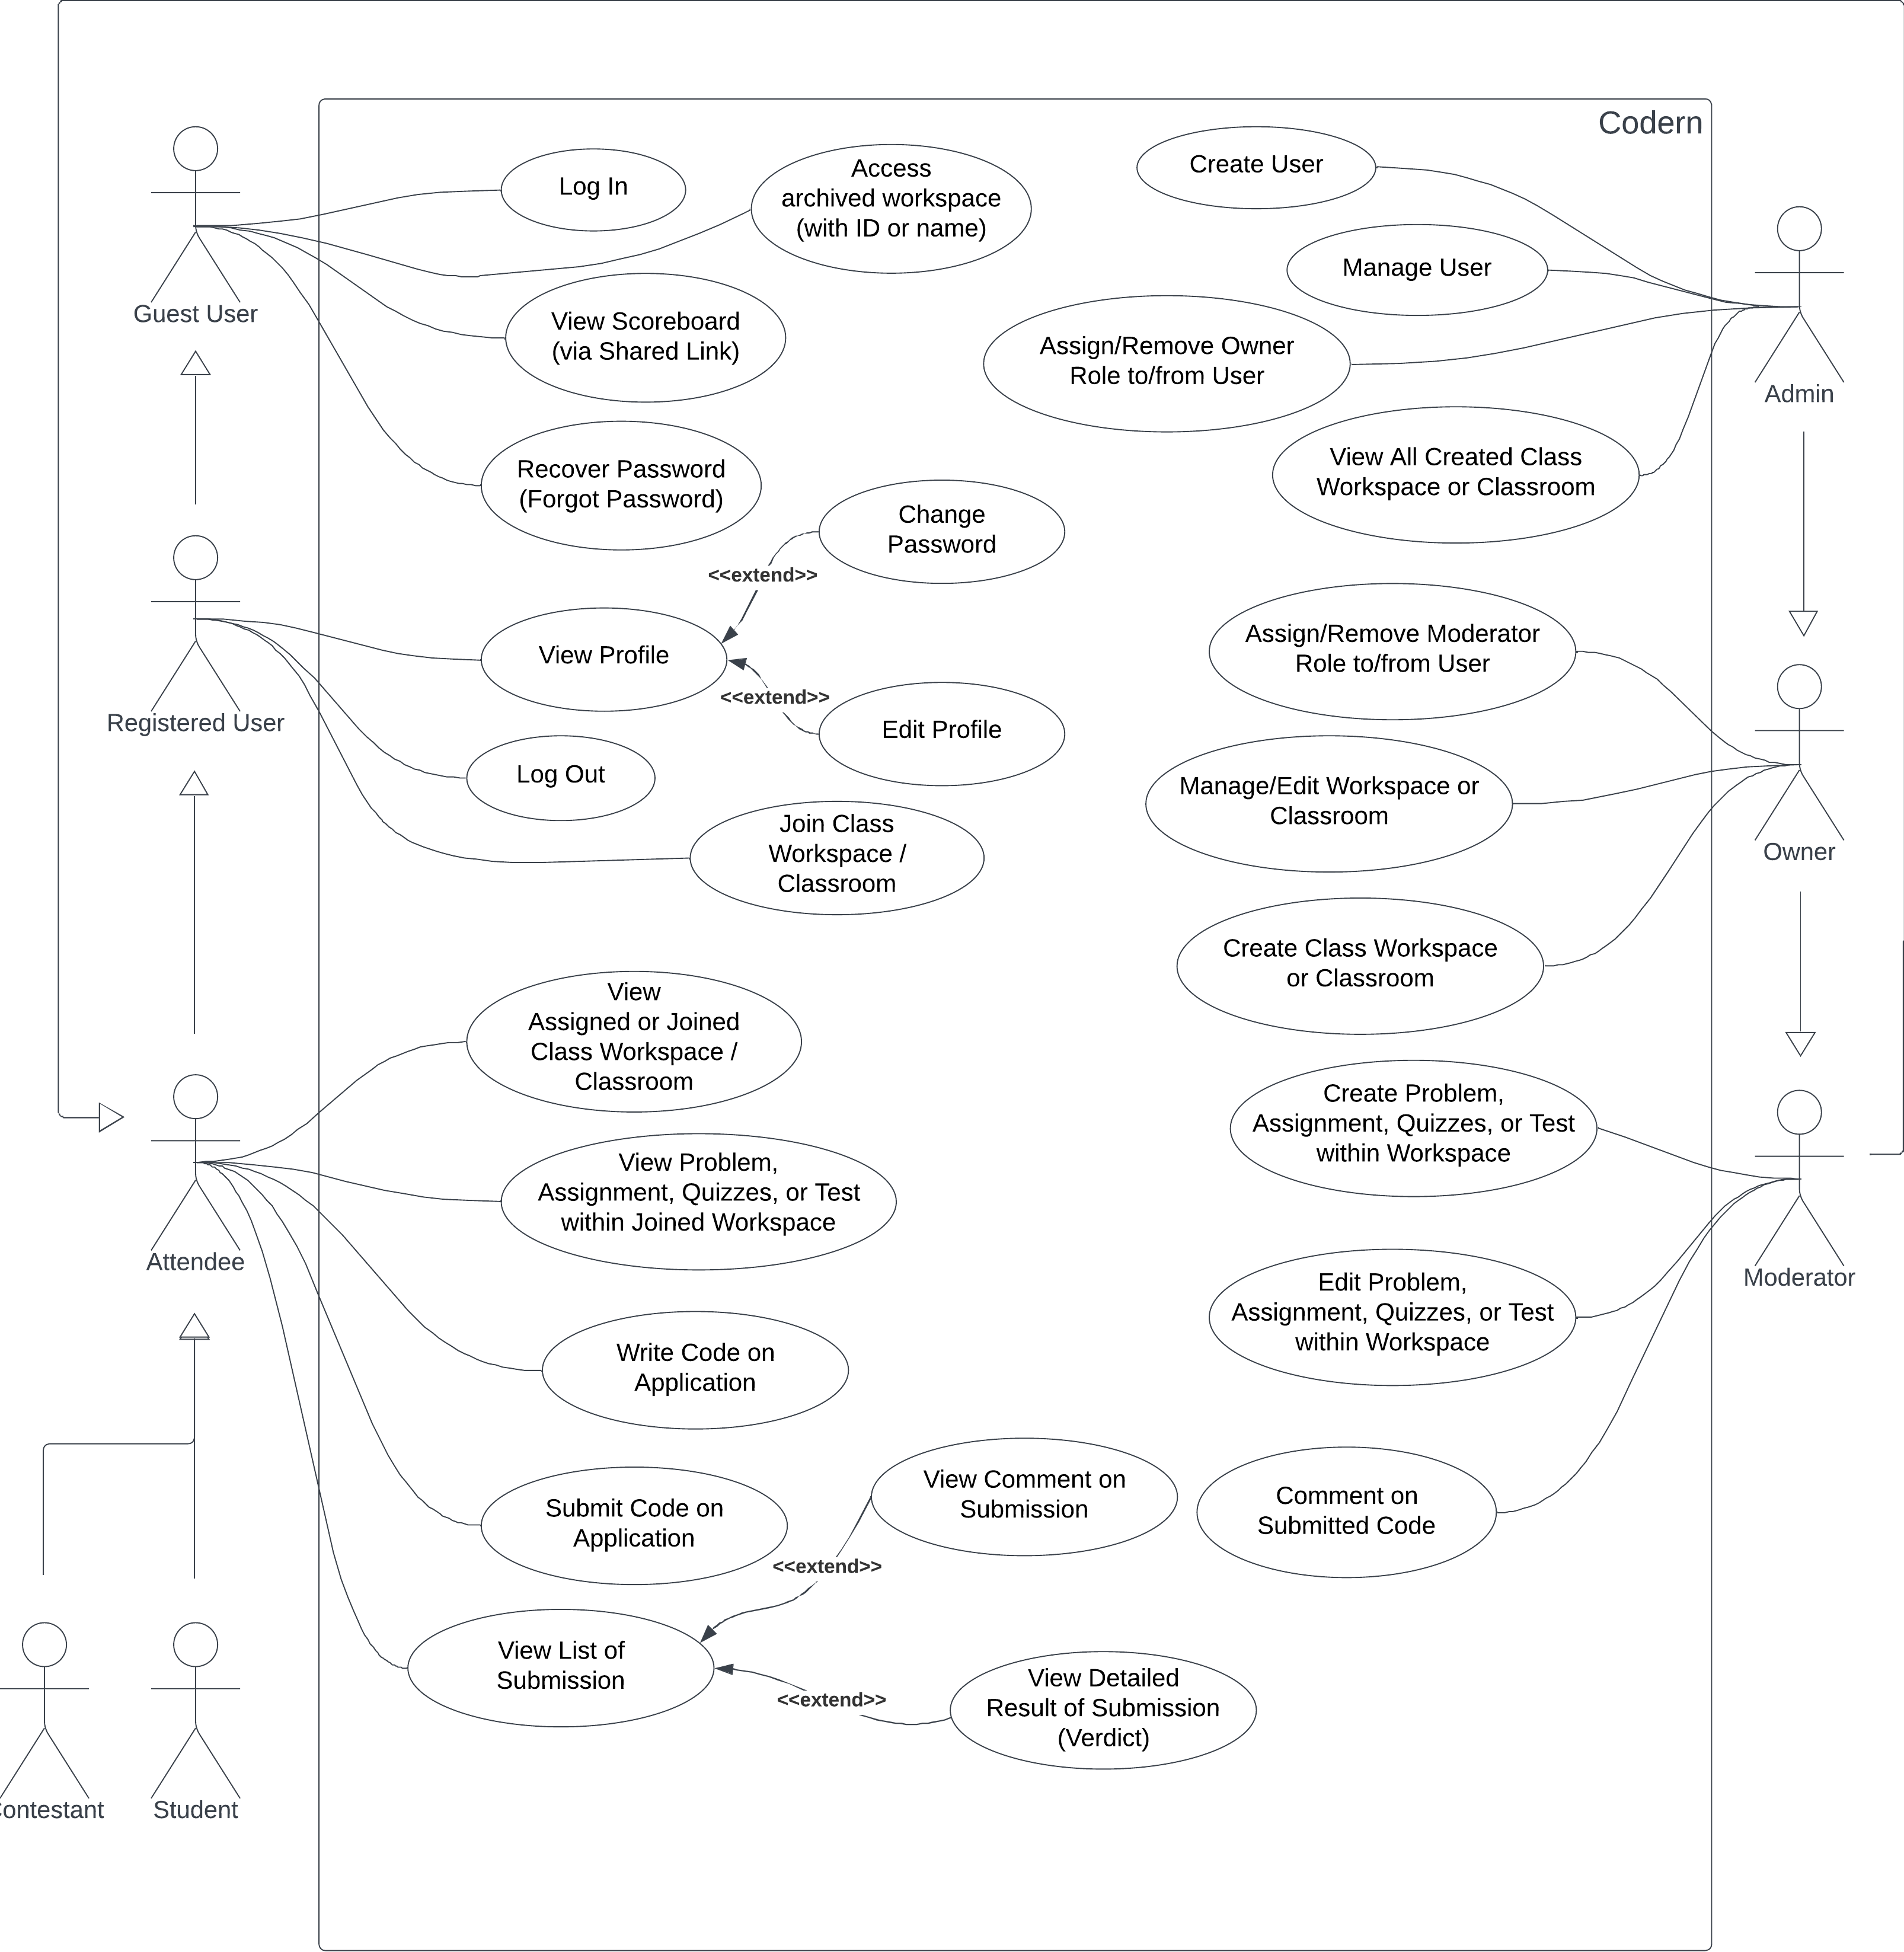
\includegraphics[width=15cm]{figure/diagram/usecase-v5.png}
    % }
    \caption[ภาพเเผนผังกรณีใช้งาน]{ภาพเเผนผังกรณีใช้งาน วาดด้วย \href{https://lucid.app/}{LucidChart}}
    \label{fig:usecase}
  \end{figure}
}
\pagebreak
\subsection{คำบรรยายแผนผังกรณีใช้งาน}
\thaijustify{
  จากรูปที่~\ref{fig:usecase} ในหัวข้อที่แล้ว เป็นรูปที่แสดงความสัมพันธ์ระหว่างผู้ใช้งานและซอฟต์แวร์ ในโครงงานซอฟต์แวร์นี้ได้แบ่งประเภทผู้ใช้ออกเป็น 6 ประเภท ได้แก่บุคคลทั่วไป (Guest User), ผู้ใช้ทั่วไป (Registered User), นักศึกษา (Student), ผู้เข้าร่วมกิจกรรมหรือการแข่งขันฯ (Attendee), เจ้าของห้องหรืออาจารย์ผู้สอน (Owner), ผู้ช่วยเจ้าของห้องหรือผู้ช่วยสอน (Moderator) และเจ้าของระบบหรือผู้ดูแลระบบ (Admin) โดยแต่ละประเภทผู้ใช้งานมีเป้าหมายหลัก และกรณีการใช้งานดังต่อไปนี้
}
\subsubsection{Guest User (บุคคลทั่วไป)}
\thaijustify{
  บุคคลทั่วไป สามารถเข้าใช้งาน feature พื้นฐานของซอฟต์แวร์ได้ดังนี้
}
\begin{enumerate}
  \item “Log In” คือ การล็อกอินเข้าสู่ระบบ
  \item “View Scoreboard (via Shared Link)” คือ การเข้าถึงตารางคะแนนด้วยลิงก์ที่ถูกแชร์มา
  \item “Recover Password” คือ การกู้คืนรหัสผ่าน กรณีที่หลงลืมหรือสูญหาย
  \item “Access Archived Workspace (with ID or Name)” คือ การเข้าถึงห้องเรียน กลุ่มเรียนเก่าที่ผู้ใช้เคยได้เข้าร่วม ที่ได้ถูกเก็บรักษาไว้ (archived) ผ่านการค้นด้วยรหัสหรือชื่อ
\end{enumerate}
\subsubsection{Registered User (ผู้ใช้ทั่วไป)}
\thaijustify{
  ผู้ใช้ทั่วไปก็คือบุคคลทั่วไปที่มีบัญชีในระบบ (Admin อาจได้สร้างไว้ให้ หรือไม่ก็สมัครเอง) โดยผู้ใช้ทั่วไปสามารถเข้าถึง feature พื้นฐานของซอฟต์แวร์ได้เหมือนกับบุคคลทั่วไป (Guest User) และยังสามารถเข้าใช้ feature เพิ่มเติมได้ดังต่อไปนี้
}
\begin{enumerate}
  \item “View Profile” คือ การเข้าดูข้อมูลส่วนตัวของตัวผู้ใช้เอง
  \item “Change Password” คือ การที่สามารถจะเปลี่ยนรหัสผ่านบัญชีตนเองได้
  \item “Edit Profile” คือ การที่สามารถจะแก้ไขข้อมูลส่วนตัวของบัญชีตนเองได้
  \item “Join Workspace” คือ การที่สามารถจะเข้าร่วมกลุ่มเรียน ห้องเรียนเองได้
  \item “Log Out” คือ การล็อกเอ้าท์ ออกจากระบบ
  \item “Create Class Workspace or Classroom” คือ การที่สามารถจะสร้างห้องเรียนหรือกลุ่มเรียนได้
\end{enumerate}
\subsubsection{Attendee (ผู้เข้าร่วมกิจกรรม)}
\thaijustify{
  ผู้เข้าร่วมกิจกรรมก็คือผู้ใช้ทั่วไปที่ได้เข้าร่วมห้องเรียนหรือกลุ่มเรียน (หรือ Workspace) อย่างน้อยหนึ่งห้อง สามารถเข้าถึง feature พื้นฐานของซอฟต์แวร์ได้เหมือนกับผู้ใช้ทั่วไป (Registered User) และยังสามารถเข้าใช้ feature เพิ่มเติมได้ดังต่อไปนี้
}
\begin{enumerate}
  \item “View Assigned or Joined Class Workspace / Classroom” คือ การเข้าถึงรายการห้องเรียน กลุ่มเรียนทั้งหมด ที่ได้เข้าร่วมหรือถูกยัดเข้า
  \item “View Problems, Assignments, Quizzes, or Tests with Joined Workspace” คือการเข้าถึงโจทย์ปัญหา และข้อสอบทั้งหมดในกลุ่มเรียนหรือห้องเรียนที่ได้เข้าร่วมหรือถูกยัดเข้า
  \item “Write Code on Application” คือ การที่สามารถจะเขียนโปรแกรมบนตัวซอฟต์แวร์ได้
  \item “Submit Code on Application” คือ การที่สามารถจะส่งโปรแกรมให้ซอฟต์แวร์ไปตรวจ
  \item “View List of Submission” คือ การเข้าถึงรายการที่แสดงการส่งโปรแกรมให้ซอฟต์แวร์ไปตรวจ ที่ตัวนักศึกษาหรือผู้เข้าร่วมกิจกรรม/การแข่งขันฯ เป็นคนส่งทั้งหมด
  \item “View Comment on Submission” คือ การเข้าถึงข้อความคิดเห็น คำแนะนำ คำติชมเกี่ยวกับงานเขียนโปรแกรมที่ได้ส่งไป ที่อาจารย์ผู้สอน ผู้ช่วยสอนได้พิมพ์เอาไว้ ในการส่งโปรแกรมที่ส่งตรวจครั้งนั้น ๆ
  \item “View Detailed Result of Submission (Verdict)” คือ การเข้าถึง รายละเอียดและผลตรวจแบบละเอียดของโปรแกรมที่ส่งตรวจในแต่ละครั้ง
\end{enumerate}
\subsubsection{Student (นักเรียนหรือนักศึกษา)}
\thaijustify{
  นักเรียนหรือนักศึกษา ก็คือผู้เข้าร่วมกิจกรรมที่ได้เข้าร่วม (joined) หรือถูกยัดเข้า (assigned) ห้องเรียน กลุ่มเรียน (workspace) ดังนั้นนักเรียนหรือนักศึกษาก็จะเข้าถึง feature พื้นฐานของซอฟต์แวร์ได้เหมือนกับผู้เข้าร่วมกิจกรรม (Attendee) เหมือนกันหมดทุกประการ
}
\subsubsection{Contestant (ผู้เข้าร่วมการแข่งขัน)}
\thaijustify{
  ผู้เข้าร่วมการแข่งขัน ก็คือผู้เข้าร่วมกิจกรรมที่ได้เข้าร่วม (joined) หรือถูกยัดเข้า (assigned) ห้องเรียน กลุ่มเรียน (workspace) เช่นเดียวกัน ดังนั้นผู้เข้าร่วมการแข่งขันเข้าถึง feature พื้นฐานของซอฟต์แวร์ได้เหมือนกับผู้เข้าร่วมกิจกรรม (Attendee) เหมือนกันหมดทุกประการ หรือได้ feature เทียบเท่ากับนักเรียนหรือนักศึกษา
}
\subsubsection{Moderator (ผู้ช่วยเจ้าของห้องหรือผู้ช่วยสอน)}
\thaijustify{
  ผู้ช่วยเจ้าของห้องหรือผู้ช่วยสอน เป็นผู้ใช้ที่ถูกเจ้าของห้องหรืออาจารย์ผู้สอนหรือเจ้าระบบแต่งตั้งให้มาเป็นผู้ช่วยบริหารห้องเรียนหรือกลุ่มเรียน ผู้ใช้หมวดหมู่นี้สามารถเข้าถึง feature ของซอฟต์แวร์ได้เหมือนกับนักศึกษาหรือผู้เข้าแข่งขันฯ (Student or Attendee) แต่ก็เข้าถึง feature เพิ่มเติมได้ดังนี้
}
\begin{enumerate}
  \item “Create Problems, Assignments, Quizzes, or Test within Workspace” คือ การที่สามารถสร้างโจทย์ปัญหา และออกข้อสอบภายในห้องเรียน หรือกลุ่มเรียนที่ตนได้คุมอยู่ได้
  \item “Edit Problems, Assignments, Quizzes, or Test within Workspace” คือ การที่สามารถจะแก้ไขโจทย์ปัญหา ออกข้อสอบภายในห้องเรียน หรือกลุ่มเรียนที่ตนได้คุมอยู่ได้
  \item “Comment on Submitted Code” คือ การที่สามารถจะให้ความเห็น ให้คำแนะนำหรือให้คำติชม แก่งานเขียนโปรแกรมที่นักศึกษา หรือผู้เข้าร่วมการแข่งขันฯ ได้ส่งเข้ามาในระบบได้
\end{enumerate}
\subsubsection{Owner (เจ้าของห้องหรืออาจารย์ผู้สอน)}
\thaijustify{
  เจ้าของห้องหรืออาจารย์ผู้สอน คือผู้ใช้ที่สามารถสร้างและบริหารจัดการห้องเรียนหรือกลุ่มเรียนได้ ผู้ใช้หมวดหมู่นี้สามารถเข้าถึง feature ของซอฟต์แวร์ได้เหมือนกับผู้ช่วยเจ้าของห้อง (Moderator) และเข้าถึง feature เพิ่มเติมได้ดังนี้
}
\begin{enumerate}
  \item “Assign/Remove Moderator Role to/from User” คือ ความสามารถที่จะแต่งตั้งหรือลดบทบาทผู้ใช้ทั่วไปให้มาเป็นผู้ช่วยสอนหรือผู้ช่วยเจ้าของห้อง (moderator)
  \item “Manage or Edit Workspace or Classroom” คือ ความสามารถที่จะแก้ไข บริหารจัดการ (ลบ) ห้องเรียนหรือกลุ่มเรียนทั้งหมดที่ตนเป็นเจ้าของ
\end{enumerate}
\subsubsection{Admin (เจ้าของระบบหรือแอดมิน)}
\thaijustify{
  เจ้าของระบบหรือแอดมิน สามารถเข้าถึง feature ของซอฟต์แวร์ได้เหมือนกับเจ้าของห้องหรืออาจารย์ผู้สอน (Owner) แต่เข้าถึง feature พิเศษเพิ่มเติมได้ ดังนี้
}
\begin{enumerate}
  \item “Create User” คือ ความสามารถในการสร้างบัญชีผู้ใช้ได้
  \item “Manage User” คือ การที่สามารถที่จะบริหารจัดการ (ลบ) ข้อมูลบัญชีผู้ใช้ทั้งหมดได้
  \item “Assign/Remove Owner Role to/from User” คือ ความสามารถที่จะแต่งตั้งหรือลดบทบาทผู้ใช้ ให้มาเป็นเจ้าของห้อง (owner)
  \item “View All Created Class Workspace or Classroom” คือ การเข้าถึงรายการแสดงผลห้องเรียนหรือกลุ่มเรียนทั้งหมดที่ได้สร้างขึ้นในระบบ
\end{enumerate}
\pagebreak

\section{สถาปัตยกรรมระบบ}
\thaijustify{
  หลังจากที่ได้ทำความเข้าใจกับข้อกำหนดและข้อใช้งานที่จำเป็นที่ผู้ใช้ต้องการแล้ว ทางกลุ่มคณะผู้จัดทำจึงได้เริ่มทำการออกแบบสถาปัตยกรรมระบบให้สอดคล้องกับข้อกำหนดในหัวข้อที่แล้ว สรุปเป็นแผนภาพในรูปที่~\ref{fig:arch} ซึ่งแผนภาพดังกล่าวเป็นแผนภาพที่แสดงสถาปัตยกรรมระบบ ที่ถูกออกแบบมาให้เป็นระบบรูปแบบกระจาย (Cluster System) ที่มีเครื่องเสมือนสองเครื่อง (Virtual Machine ในรูปเรียกโดยย่อว่า \textit{VM1} และ \textit{VM2}) จากในรูปจะเรียกระบบกระจายนี้ว่า \textit{Codern Cluster}
}
%%%%%%%%%%% ARCHITECTURE DIAGRAM %%%%%%%%%%%
\begin{figure}[!h]
  \centering
  % \fbox{
  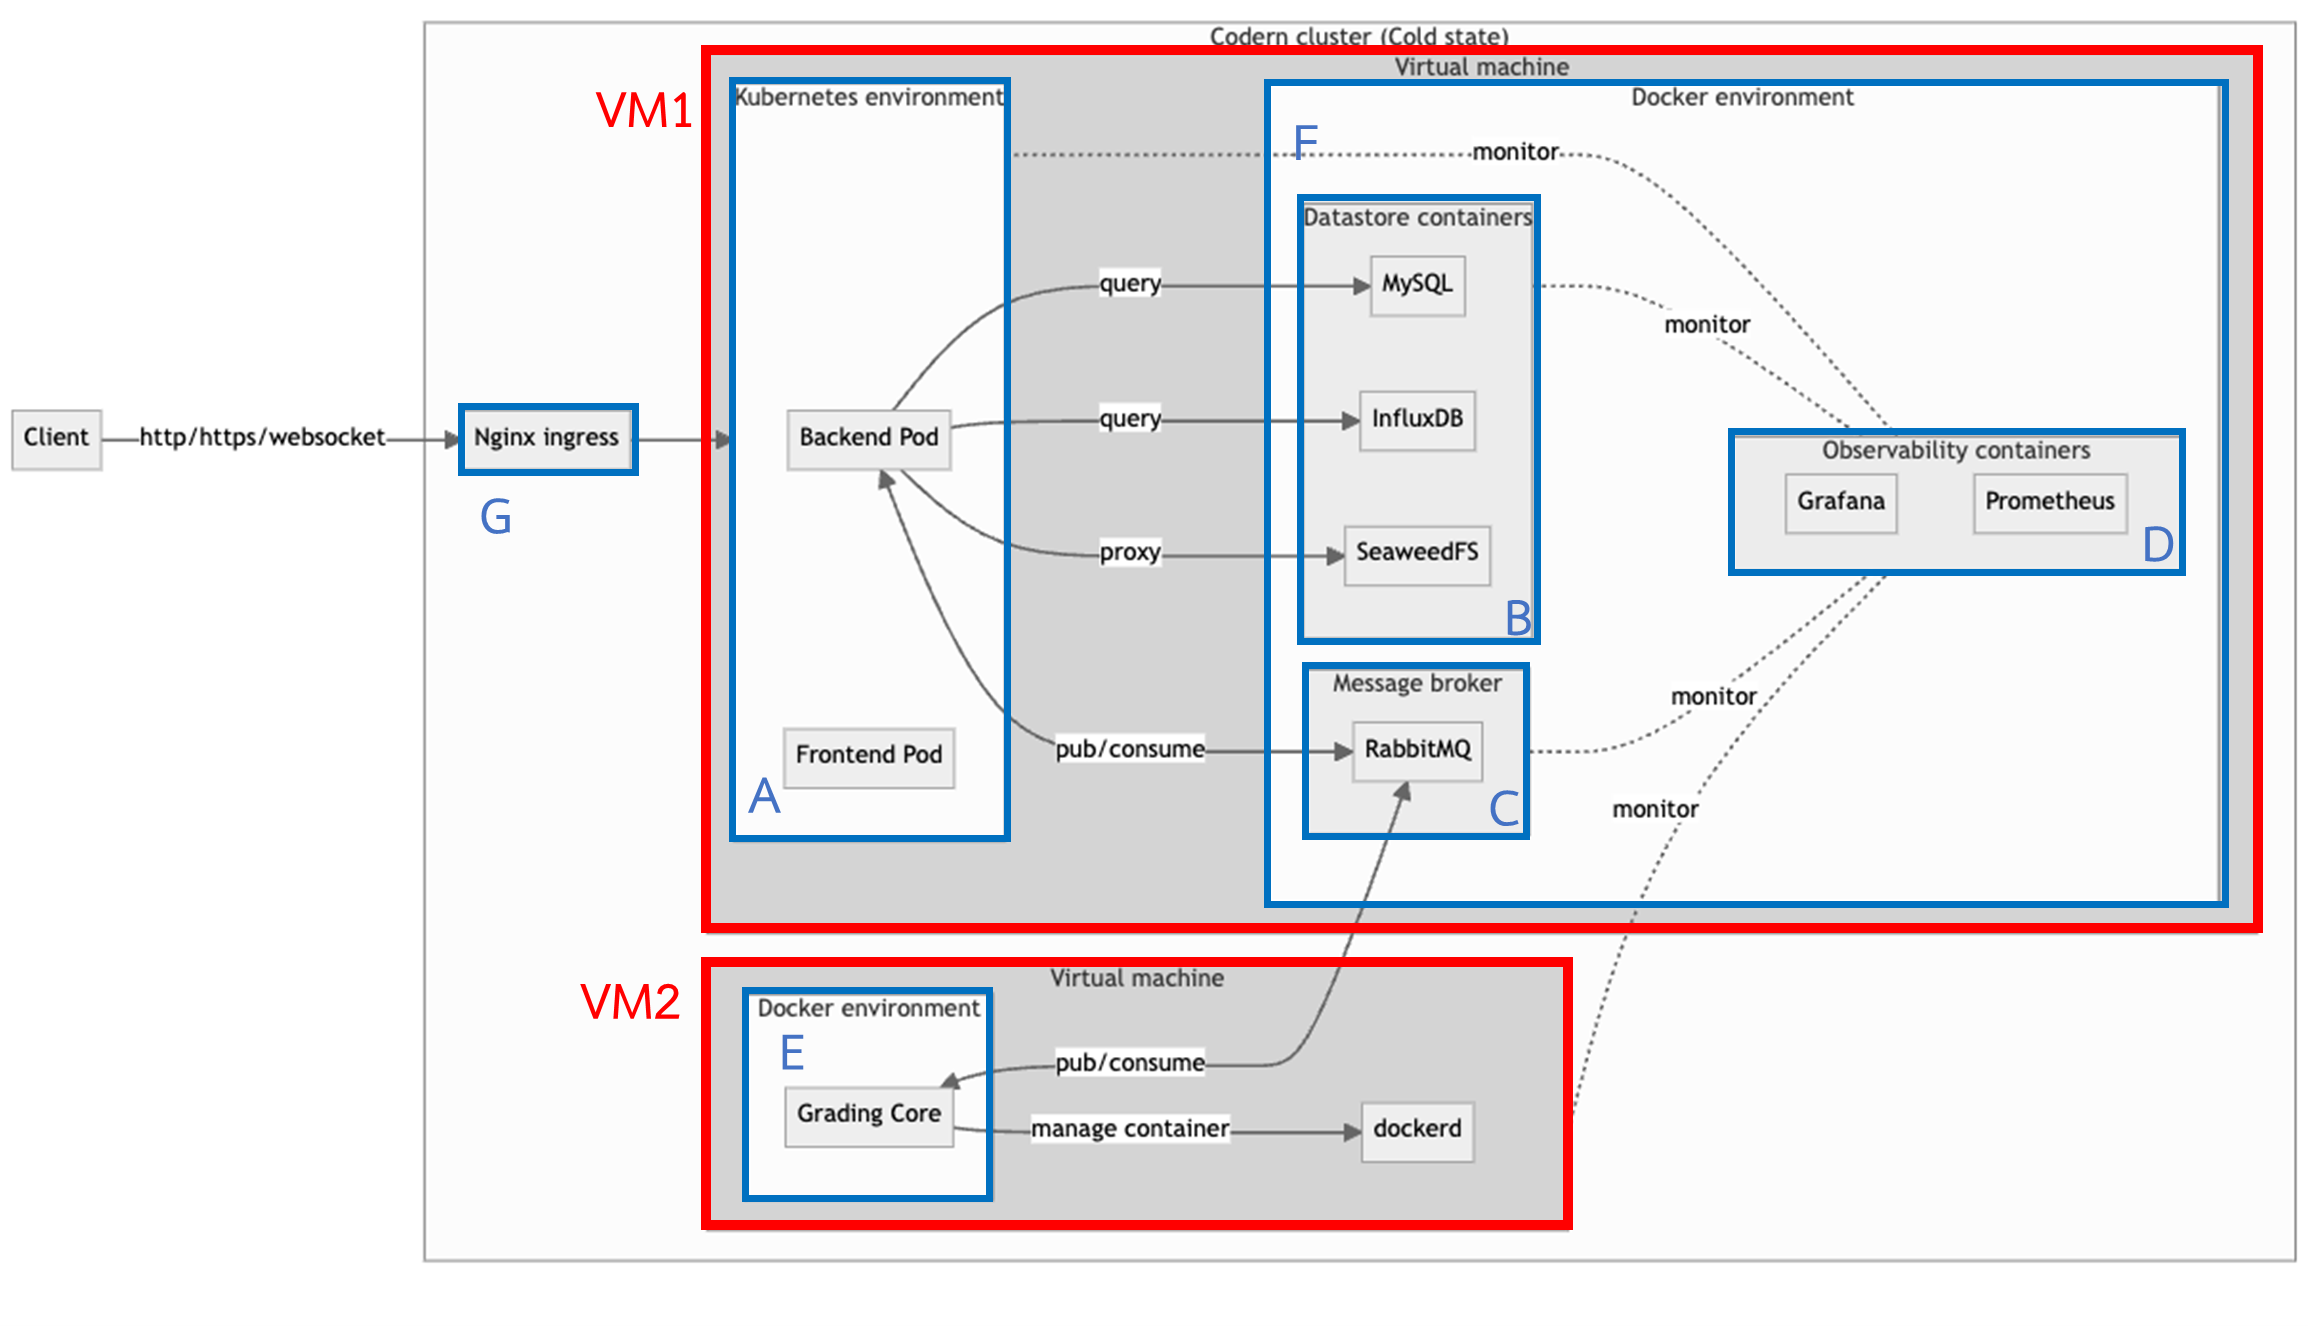
\includegraphics[width=15cm]{figure/diagram/architecture-v1.png}
  % }
  \caption[ภาพเเผนผังสถาปัตยกรรมระบบของซอฟต์เเวร์]{ภาพเเผนผังสถาปัตยกรรมระบบของซอฟต์เเวร์ วาดด้วย \href{https://mermaid.js.org/}{Mermaid JS}}\label{fig:arch}
\end{figure}
% TODO: Detailed writing for Architectures
% \thaijustify{
%     จากสถาปัตยกรรมระบบที่ได้ออกแบบไว้ในหัวข้อสถาปัตยกรรมระบบ การใช้ตัวประสานงานหรือ “์Nginx Ingress” ในรูปที่~\ref{fig:arch} ระหว่างฝั่งผู้ใช้กับระบบ จะสามารถแบ่งเบาและแจกจ่ายคำขอจากผู้ใช้อย่างมีประสิทธิภาพ และอีกทั้งการใช้ตัวสื่อสาร (Message Broker หรือ “RabbitMQ” ในรูปที่~\ref{fig:arch}) ระหว่างตัวซอฟต์แวร์หลักกับตัวโมดูลตรวจงานเขียนโปรแกรม (Grading Core) จะทำให้การจัดการคิวคำขอตรวจงานเขียนโปรแกรมง่ายขึ้น  ทำให้การตรวจให้คะแนน ประกาศผลคะแนนและบันทึกลงฐานข้อมูล ดำเนินการตามลำดับอย่างต่อเนื่อง
% }
% \thaijustify{
%     จากเหตุผลข้างต้น ในเชิงอดุมคติ ซอฟต์แวร์ที่ทางกลุ่มผู้จัดทำโครงการออกแบบมาจะสามารถรับมือกับคำขอจากฝั่งผู้ใช้ได้จำนวนมหาศาล รองรับจำนวนผู้ใช้เข้ามาใช้งานในระบบพร้อมกันได้จำนวนมาก
% }
\thaijustify{
  ใน VM1 มีการวางรูปแบบซอฟต์แวร์เป็นรูปแบบ Kubernetes (กรอบ A ในรูป) ที่มี pod ชื่อ Backend Pod และ Frontend Pod โดย Pod เหล่านี้จะติดต่อสื่อสารกับส่วนประกอบต่างอื่นๆ ใน Container ที่ Host โดย Docker ในเครื่องเดียวกัน Docker (กรอบ F ในรูป) ในเครื่อง VM1 จะ host คอนเทนเนอร์ 3 อัน ได้แก่แหล่งเก็บข้อมูลหรือฐานข้อมูลต่าง ๆ (กรอบ B) อาทิเช่น MySQL, InfluxDB และ SeaweedFS, ตัว Message Broker (กรอบ C) หรือ RabbitMQ ซึ่งก็คือโมดูล ที่เปิดบริการสำหรับการส่งข้อมูลและสื่อสารไปยัง VM2 เพื่อส่งไฟล์โปรแกรมไปตรวจ และสุดท้ายก็คือ Monitoring Tool อย่าง Grafana และ Prometheus (กรอบ D) ซึ่งเป็นเครื่องมือสำหรับการตรวจดู สอดส่องดูแล วิเคราะห์หาข้อบกพร่อง และวัดประสิทธิภาพการทำงานของแต่ละส่วนของซอฟต์แวร์
}
\thaijustify{
  ใน VM2 ก็มี Docker ที่ Host ตัว Container อยู่เช่นกัน โดย Container นี้จะเปิด Grading Core ไว้ ซึ่งทำหน้าที่เป็นตัวโมดูลโปรแกรมสำหรับตรวจไฟล์โปรแกรมที่ผู้ใช้ได้ส่งเข้ามาจาก VM1 ผ่าน Message Broker หลังจากตรวจเสร็จก็จะส่งผลตรวจกลับไปยัง Message Broker
}
\thaijustify{
  คำขอของผู้ใช้จะถูกประมวลผลโดยตัวควบคุม Nginx Ingress (กรอบ G ในรูป) เพื่อส่งคำขอของ Client ไป Kubernetes cluster ที่ได้ host ไว้ เพื่อประมวลผล
}
\pagebreak
\section{ส่วนประสานต่อผู้ใช้}
\thaijustify{
  สำหรับในส่วนหน้าประสานงานผู้ใช้หรือ User Interface (UI) ทางคณะผู้จัดทำจะนำเสนอหน้าส่วนประสานต่อผู้ใช้ที่ได้ออกแบบไว้ทั้งหมด ดังนี้
}
%%%%%%%%%%% LOGIN %%%%%%%%%%%
\hypertarget{ui-login}{
  \begin{figure}[H]
    \centering
    \includegraphics[width=15cm]{figure/ui/ui-login1.png}
    \caption[ส่วนประสานต่อผู้ใช้ หน้าเข้าสู่ระบบ]{ส่วนประสานต่อผู้ใช้ หน้าเข้าสู่ระบบ}
    \label{fig:ui-login}
  \end{figure}
}

\thaijustify{
  ในรูปที่~\ref{fig:ui-login} เป็นหน้าสำหรับล็อกอินเข้าระบบใช้งานทั้งหมดของซอฟต์แวร์ โดยสามารถเลือกล็อกอินได้สองวิธี; ด้วยอีเมลเเละรหัสผ่าน (กรอบสีน้ำเงิน A) และล็อกอินผ่านกูเกิ้ล (กรอบสีแดง B)
}

%%%%%%%%%%% DASHBOARD %%%%%%%%%%%
\hypertarget{ui-dashboard1}{
  \begin{figure}[H]
    \centering
    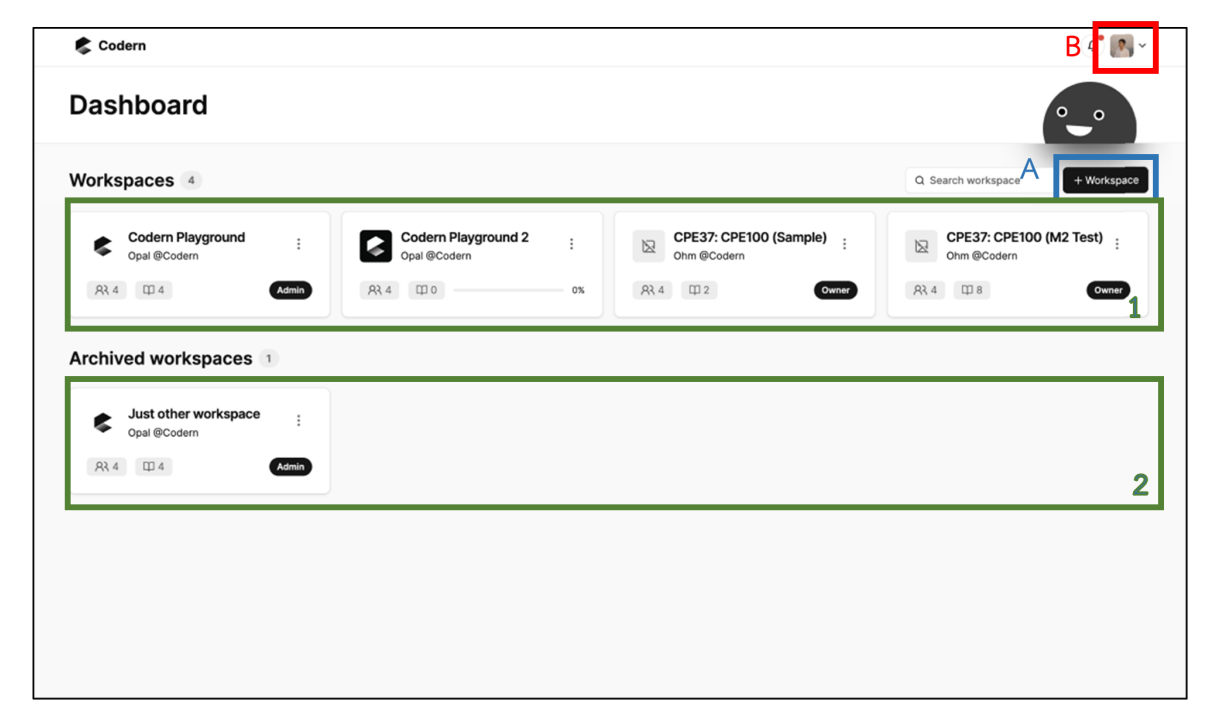
\includegraphics[width=15cm]{figure/ui/ui-dashboard1.png}
    \caption[ส่วนประสานต่อผู้ใช้ หน้าแผงควบคุม]{ส่วนประสานต่อผู้ใช้ หน้าแผงควบคุม}
    \label{fig:ui-dashboard1}
  \end{figure}
}

\thaijustify{
  เมื่อเข้าสู่ระบบเรียบร้อยแล้ว จากนั้นจะไปสู่หน้าแสดงรายการห้องทั้งหมดที่ผู้ใช้ได้เข้าร่วม ดังรูปที่~\ref{fig:ui-dashboard1} ส่วนต่อประสานกับผู้ใช้หน้าแสดงรายการห้องที่ผู้ใช้ได้เข้าร่วมอยู่ มีทั้งการแสดงห้องเรียนหรือกลุ่มเรียนทั้งหมดที่เคยเข้าร่วมในส่วน “All Workspaces” (โซนที่ 1) และแสดงห้องเรียนหรือกลุ่มเรียนที่ได้สิ้นสุดคอร์สเรียนหรือสิ้นสุดการใช้งานไปแล้วในส่วน “Archived workspaces” (โซนที่ 2) ผู้ใช้สามารถที่จะกดเข้าร่วมห้องใหม่ได้ที่ปุ่ม “Add Workspace” ตรงมุมขวาบนในกรอบสีน้ำเงิน A และสามารถกดเพื่อแก้ไขข้อมูลเกี่ยวกับบัญชีของตัวเองได้ที่ปุ่มไอคอนอวาตาร์รูปของตนบริเวณมุมขวาบนสุดในกรอบสีแดง B

}

\hypertarget{ui-dashboard2}{
  \begin{figure}[H]
    \centering
    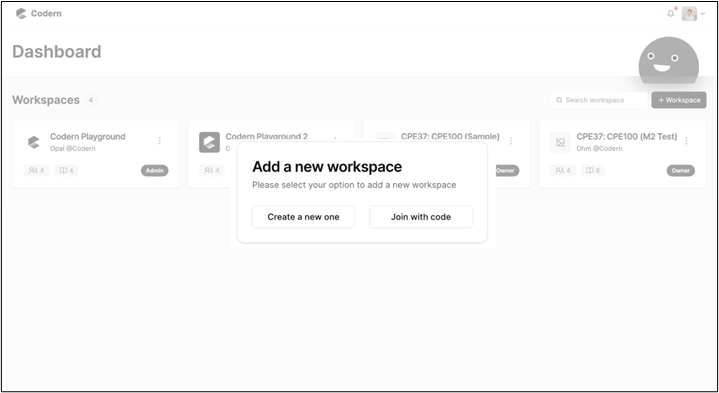
\includegraphics[width=15cm]{figure/ui/ui-dashboard2.png}
    \caption[ส่วนประสานต่อผู้ใช้ หน้าแผงควบคุม (กดเพิ่ม Workspace)]{ส่วนประสานต่อผู้ใช้ หน้าเเผงควบคุม หลังกดปุ่มเพิ่ม Workspace}
    \label{fig:ui-dashboard2}
  \end{figure}
}
\thaijustify{
  โดยเมื่อผู้ใช้กดเข้าร่วมห้องใหม่ที่ปุ่ม “Add Workspace” แล้ว จะปรากฏกล่องข้อความแจ้งเตือนเพื่อแสดงสองทางเลือก ดังรูปที่~\ref{fig:ui-dashboard2} ได้แก่ “Create a new one” ซึ่งผู้ใช้จะสามารถกดเพื่อเข้าสู่หน้าการสร้างห้องเรียนใหม่ โดยกรอกข้อมูลชื่อของห้องเรียน รายละเอียดและรูปภาพ เมื่อกดปุ่ม "Create a new one" แล้ว ห้องเรียนก็จะถูกสร้าง ดังรูปที่~\ref{fig:ui-dashboard3} และ “Join with code” ซึ่งผู้ใช้สามารถกดเพื่อกรอกรหัสเข้าร่วมห้องเรียนที่ได้มีการสร้างไว้ก่อนอยู่แล้วได้ ดังรูปที่~\ref{fig:ui-dashboard4}
}


%%%%%%%%%%% CREATE WORKSPACE %%%%%%%%%%%
\hypertarget{ui-dashboard3}{
  \begin{figure}[H]
    \centering
    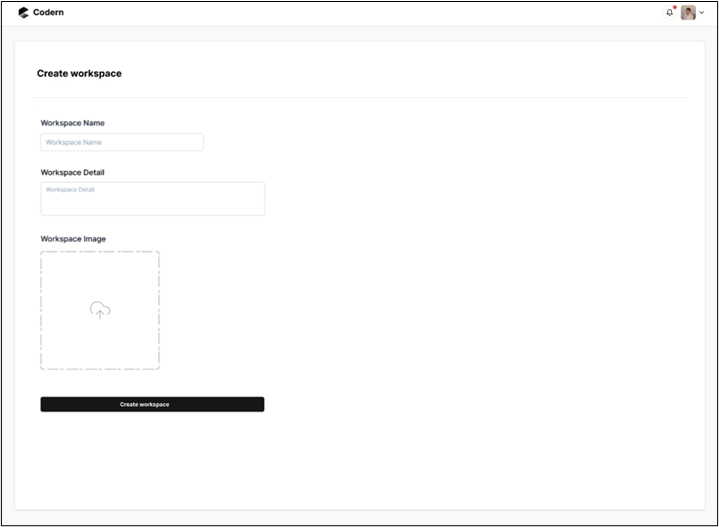
\includegraphics[width=15cm]{figure/ui/ui-dashboard3.png}
    \caption[ส่วนประสานต่อผู้ใช้ หน้าเเผงควบคุม (กดปุ่ม "Create a new one")]{ ส่วนประสานต่อผู้ใช้ หน้าเเผงควบคุม หลังกดปุ่ม "Create a new one"}
    \label{fig:ui-dashboard3}
  \end{figure}
}

\hypertarget{ui-dashboard4}{
  \begin{figure}[H]
    \centering
    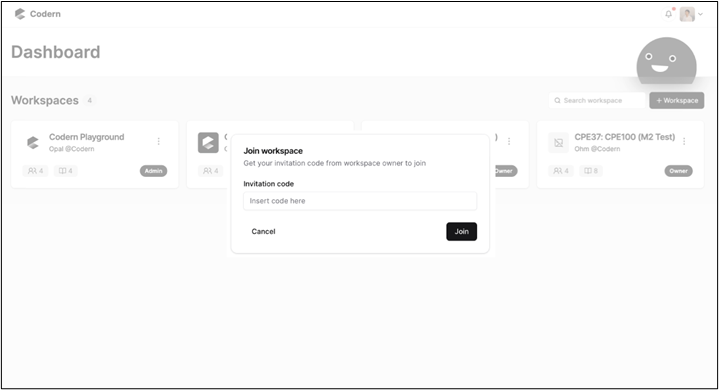
\includegraphics[width=15cm]{figure/ui/ui-dashboard4.png}
    \caption[ส่วนประสานต่อผู้ใช้ หน้าเเผงควบคุม (กดปุ่ม "Join with code")]{ส่วนประสานต่อผู้ใช้ หน้าเเผงควบคุม หลังกดปุ่ม "Join with code" }
    \label{fig:ui-dashboard4}
  \end{figure}
}

\hypertarget{ui-dashboard5}{
  \begin{figure}[H]
    \centering
    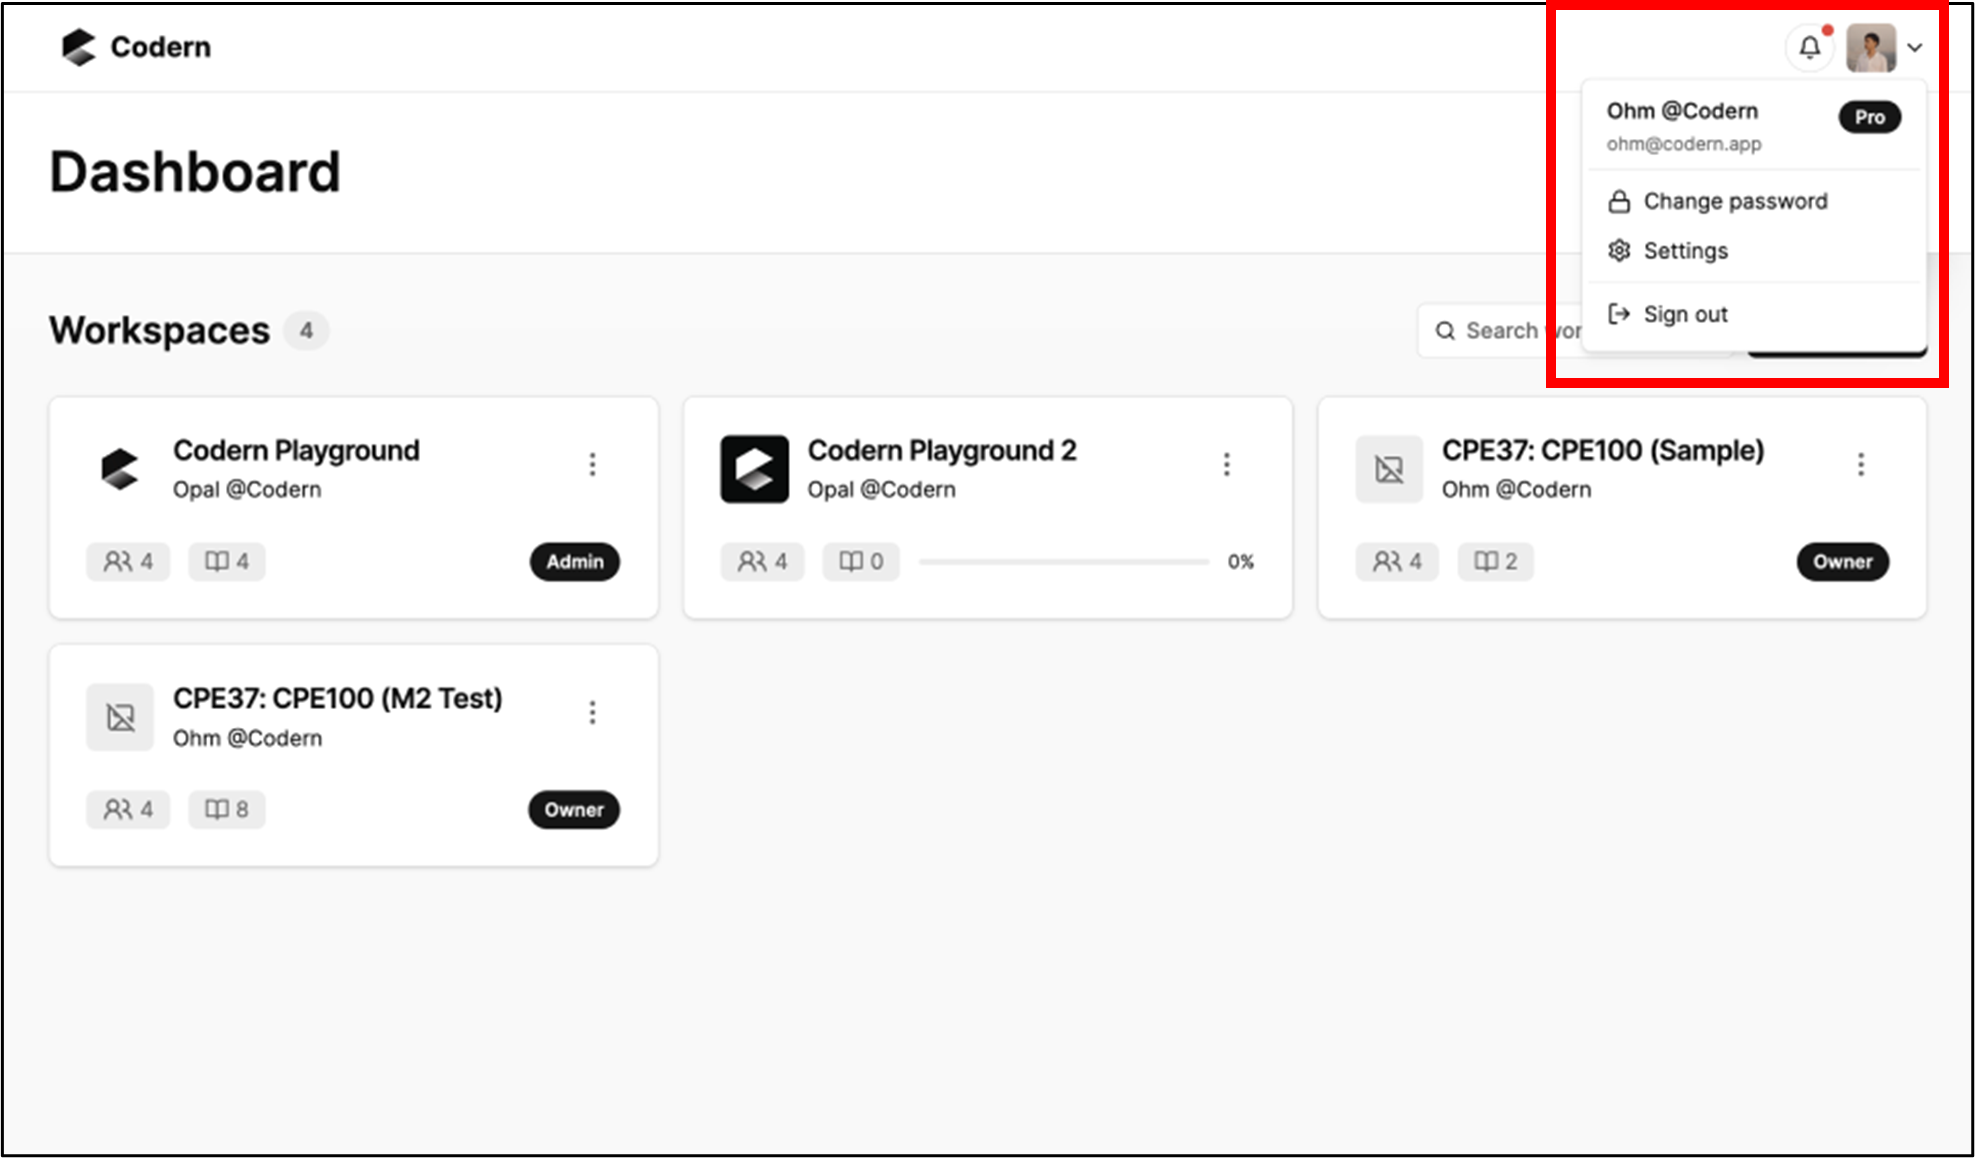
\includegraphics[width=15cm]{figure/ui/ui-dashboard5.png}
    \caption[ส่วนประสานต่อผู้ใช้ หน้าเเผงควบคุม (กดตรงรูป Avatar)]{ ส่วนประสานต่อผู้ใช้ หน้าเเผงควบคุม หากกดรูป Avatar ตรงมุมขวาบน}
    \label{fig:ui-dashboard5}
  \end{figure}
}

\thaijustify{
  หากกดปุ่มไอคอนอวาตาร์รูปของตนบริเวณมุมขวาบนสุดในกรอบสีแดง B ในรูปที่~\ref{fig:ui-dashboard2} ก็จะปรากฏ Dropdown ลงมาดังรูปที่~\ref{fig:ui-dashboard5} (กรอบสีแดง) ประกอบด้วย 3 เมนู ได้แก่ "Change password", "Settings" และ "Sign out"

}

%%%%%%%%%%% SETTINGS %%%%%%%%%%%
\hypertarget{ui-settings-password}{
  \begin{figure}[H]
    \centering
    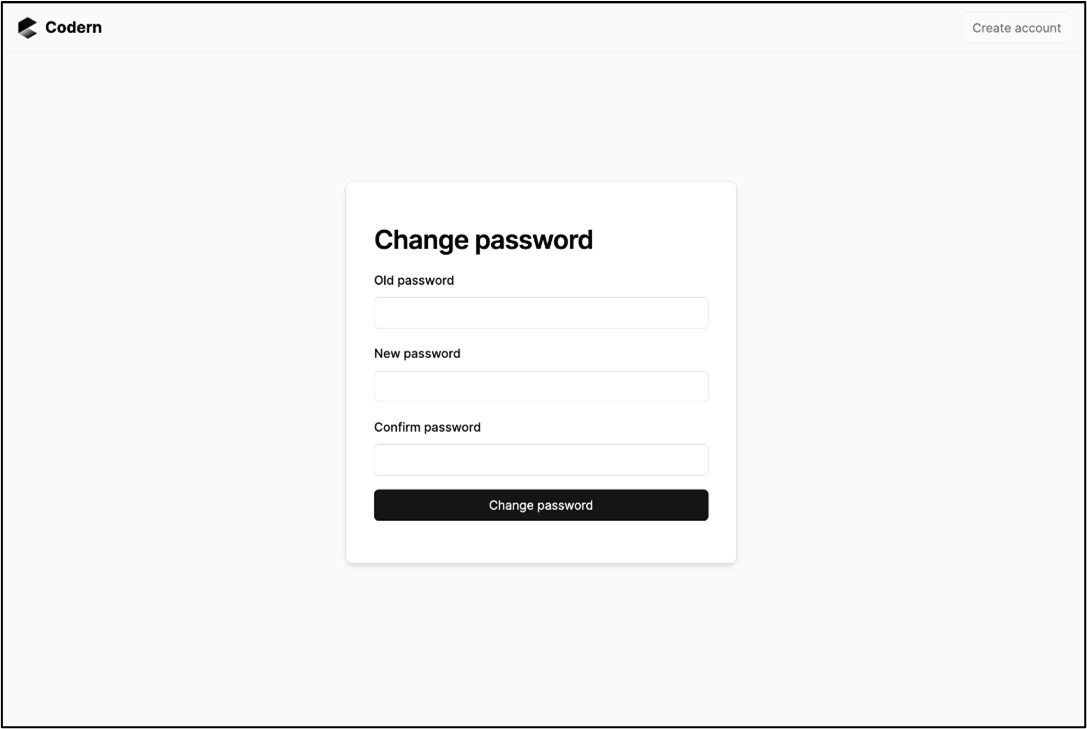
\includegraphics[width=15cm]{figure/ui/ui-settings-password.png}
    \caption[ส่วนประสานต่อผู้ใช้ หน้าตั้งค่าของผู้ใช้ (กดปุ่ม "Change Password")]{ ส่วนประสานต่อผู้ใช้ หน้าเเผงควบคุม หากกดปุ่ม "Change Password"}
    \label{fig:ui-settings-password}
  \end{figure}
}
\thaijustify{
  เมื่อกดปุ่ม "Change password" ในรูปที่~\ref{fig:ui-dashboard5} จะนำไปสู่หน้าเปลี่ยนรหัสผ่านเข้าบัญชี ดังรูปที่~\ref{fig:ui-settings-password} โดยจะเปลี่ยนรหัสผ่านบัญชีได้โดยการกรอกรหัสผ่านเก่าให้ถูกต้อง จากนั้นก็กรอกรหัสผ่านใหม่ที่ต้องการ และทำการยืนยันรหัสผ่านใหม่ซ้ำอีกครั้ง เมื่อกรอกรหัสทั้งหมดถูกต้อง เพียงกดปุ่ม "Change password" ก็จะสามารถเปลี่ยนรหัสผ่านบัญชีใหม่ได้
}
\thaijustify{
  ถ้ากดปุ่ม "Settings" ในรูปที่~\ref{fig:ui-dashboard5} จะนำไปสู่หน้าแก้ไขข้อมูลส่วนตัวของเจ้าของบัญชี ได้แก่ ชื่อบัญชี และรูปภาพอวาตาร์ ดังรูปที่~\ref{fig:ui-settings} แต่ถ้ากดปุ่ม Sign out ในรูปที่~\ref{fig:ui-dashboard5} จะกลับไปสู่หน้าล็อกอินแรกสุดของระบบ ดังรูปที่~\ref{fig:ui-login}
}
\hypertarget{ui-settings}{
  \begin{figure}[H]
    \centering
    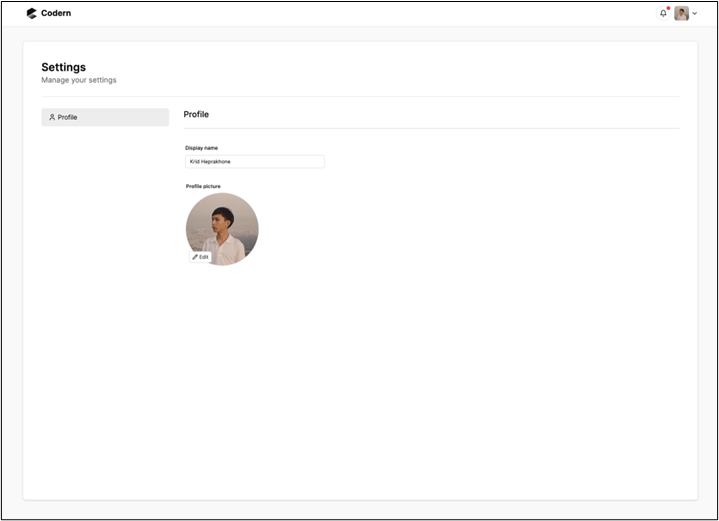
\includegraphics[width=15cm]{figure/ui/ui-settings.png}
    \caption[ส่วนประสานต่อผู้ใช้ หน้าตั้งค่าของผู้ใช้ (กดปุ่ม "Settings")]{ส่วนประสานต่อผู้ใช้ หน้าตั้งค่าของผู้ใช้ หากกดปุ่ม "Settings"}
    \label{fig:ui-settings}
  \end{figure}
}
\thaijustify{
  หากเป็นผู้ดูแล ในการแสดงรายการห้องทั้งหมด จะเปลี่ยนเป็นมุมมองของผู้ดูแลระบบดังรูปที่~\ref{fig:ui-org-dashboard1} แผงควบคุมดังกล่าว มีบทบาทและการจัดวางที่คล้ายคลึงกันกับฝั่งของผู้ใช้ทั่วไปในรูปที่~\ref{fig:ui-dashboard1} ต่างกันที่การจัดหมวดหมู่ห้องเรียน ทั้งนี้ก็จะมีปุ่มกดที่มุมขวาบนเป็นปุ่มที่สำคัญที่สุดก็คือ “Create Workspace” ที่เป็นปุ่มในการสร้างห้องเรียนหรือกลุ่มเรียนใหม่ (กรอบสีแดง A ในรูป ~\ref{fig:ui-org-dashboard1}) ซึ่งหากกดต่อไป ก็จะไปสู่หน้าสร้างห้องเรียนหรือกลุ่มเรียนใหม่เหมือนกับในรูปที่~\ref{fig:ui-dashboard3}
}
\hypertarget{ui-org-dashboard1}{
  \begin{figure}[H]
    \centering
    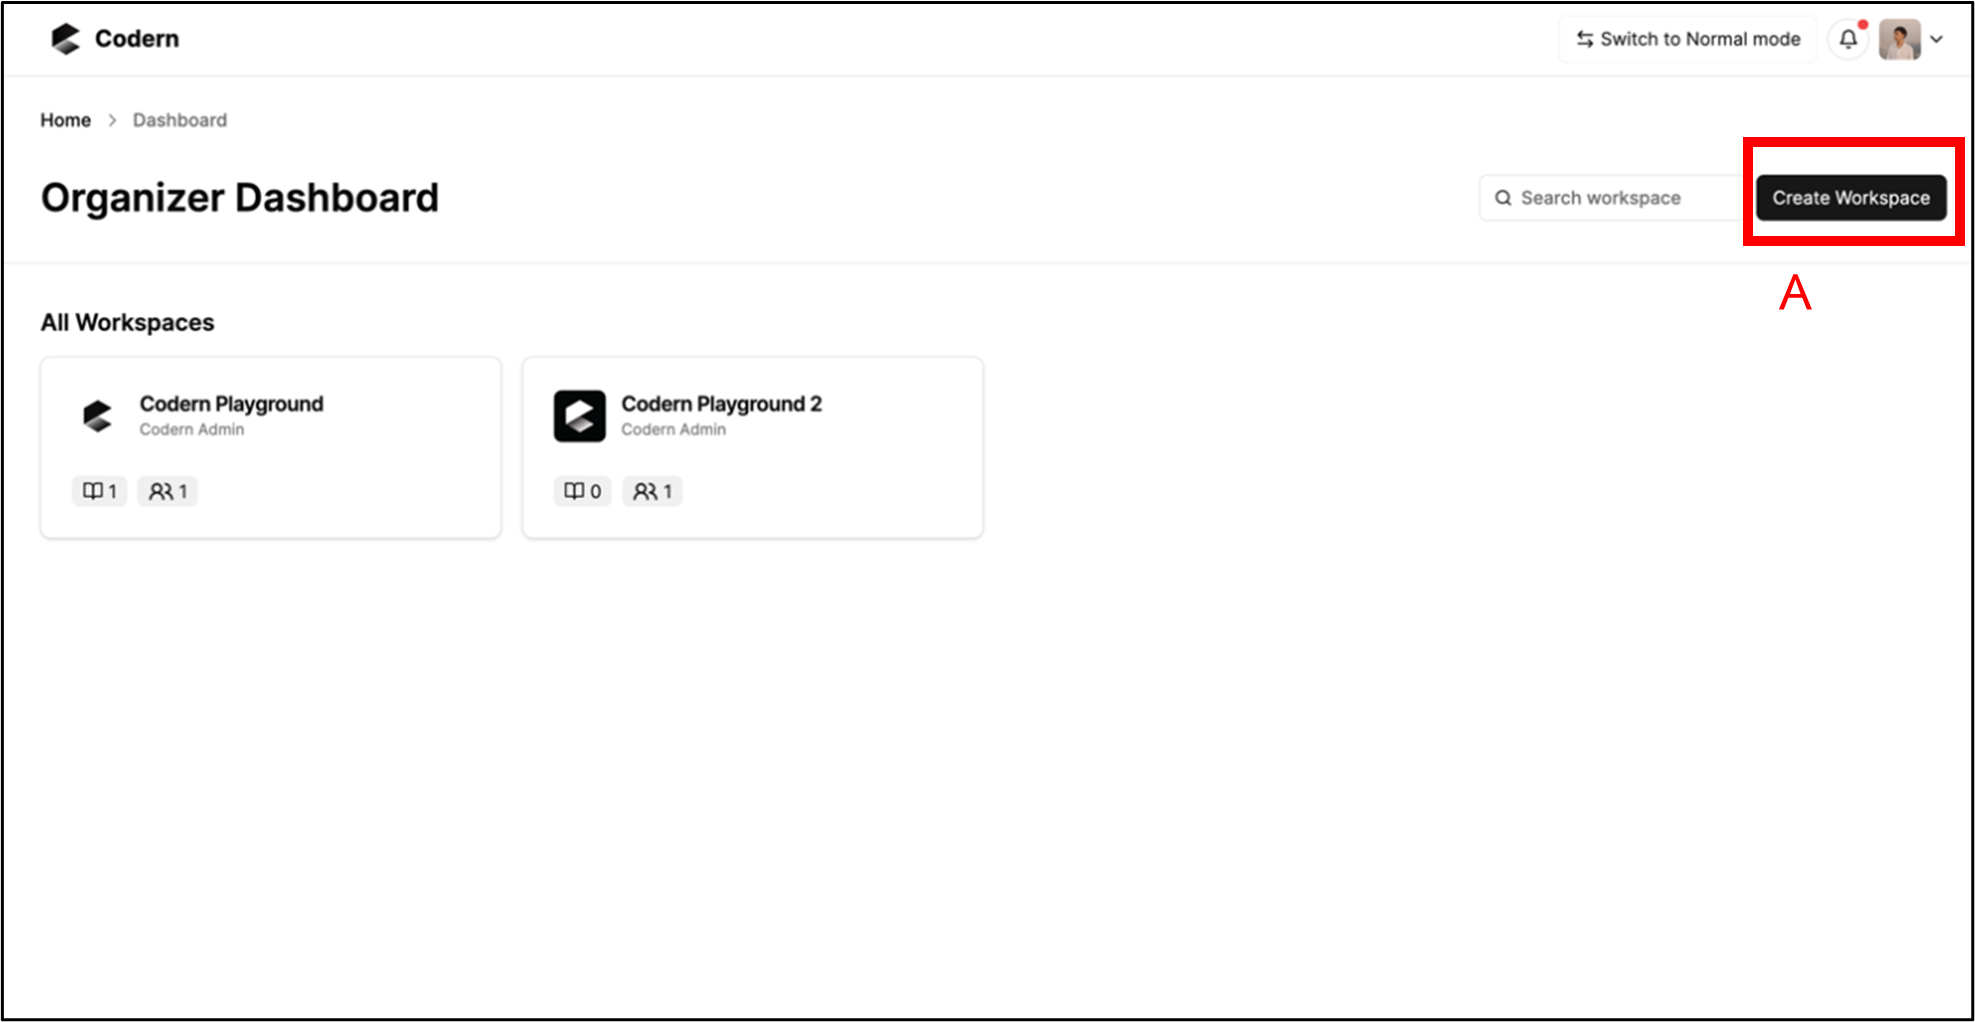
\includegraphics[width=15cm]{figure/ui/ui-org-dashboard1.png}
    \caption[ส่วนประสานต่อผู้ใช้ หน้าแผงควบคุม ในมุมมองของผู้ดูแลระบบ]{ส่วนประสานต่อผู้ใช้ หน้าเเผงควบคุมในมุมมองของผู้ดูเเลระบบ}
    \label{fig:ui-org-dashboard1}
  \end{figure}
}
%%%%%%%%%%% ASSIGNMENT LIST %%%%%%%%%%%
\thaijustify{
  ถ้าหากกดเข้าห้องเรียนหรือกลุ่มเรียนใด ๆ ในหน้าก่อน (ในรูปที่~\ref{fig:ui-dashboard1}) ก็จะนำมาสู่หน้าจอ ดังรูปที่~\ref{fig:ui-assign1} (หรือรูปที่~\ref{fig:ui-assign2} ถ้าหากเป็นแอดมินหรือผู้ดูแล) โดยในหน้านี้ ที่โซนที่ 1 จะแสดงโจทย์ปัญหา การบ้านหรือข้อสอบทั้งหมดที่เจ้าของห้อง/อาจารย์ผู้สอนได้สร้างไว้ แต่ละรายการก็จะแสดงข้อมูลตั้งแต่ชื่องาน, รายละเอียดงาน, ระดับความยาก, จนไปถึงสถานะ นอกจากแสดงโจทย์แล้ว ในส่วนบน ตรงโซนที่ 2 ยังมีการแสดงข้อมูลของห้องเรียนหรือกลุ่มเรียนด้วย ตั้งแต่ชื่อเจ้าของห้อง จำนวนงานในกลุ่มหรือห้อง จำนวนงานที่ผู้ใช้ยังทำไม่เสร็จจำนวนสมาชิกที่ได้เข้าร่วมห้องหรือกลุ่มนี้
}
\hypertarget{ui-assign1}{
  \begin{figure}[H]
    \centering
    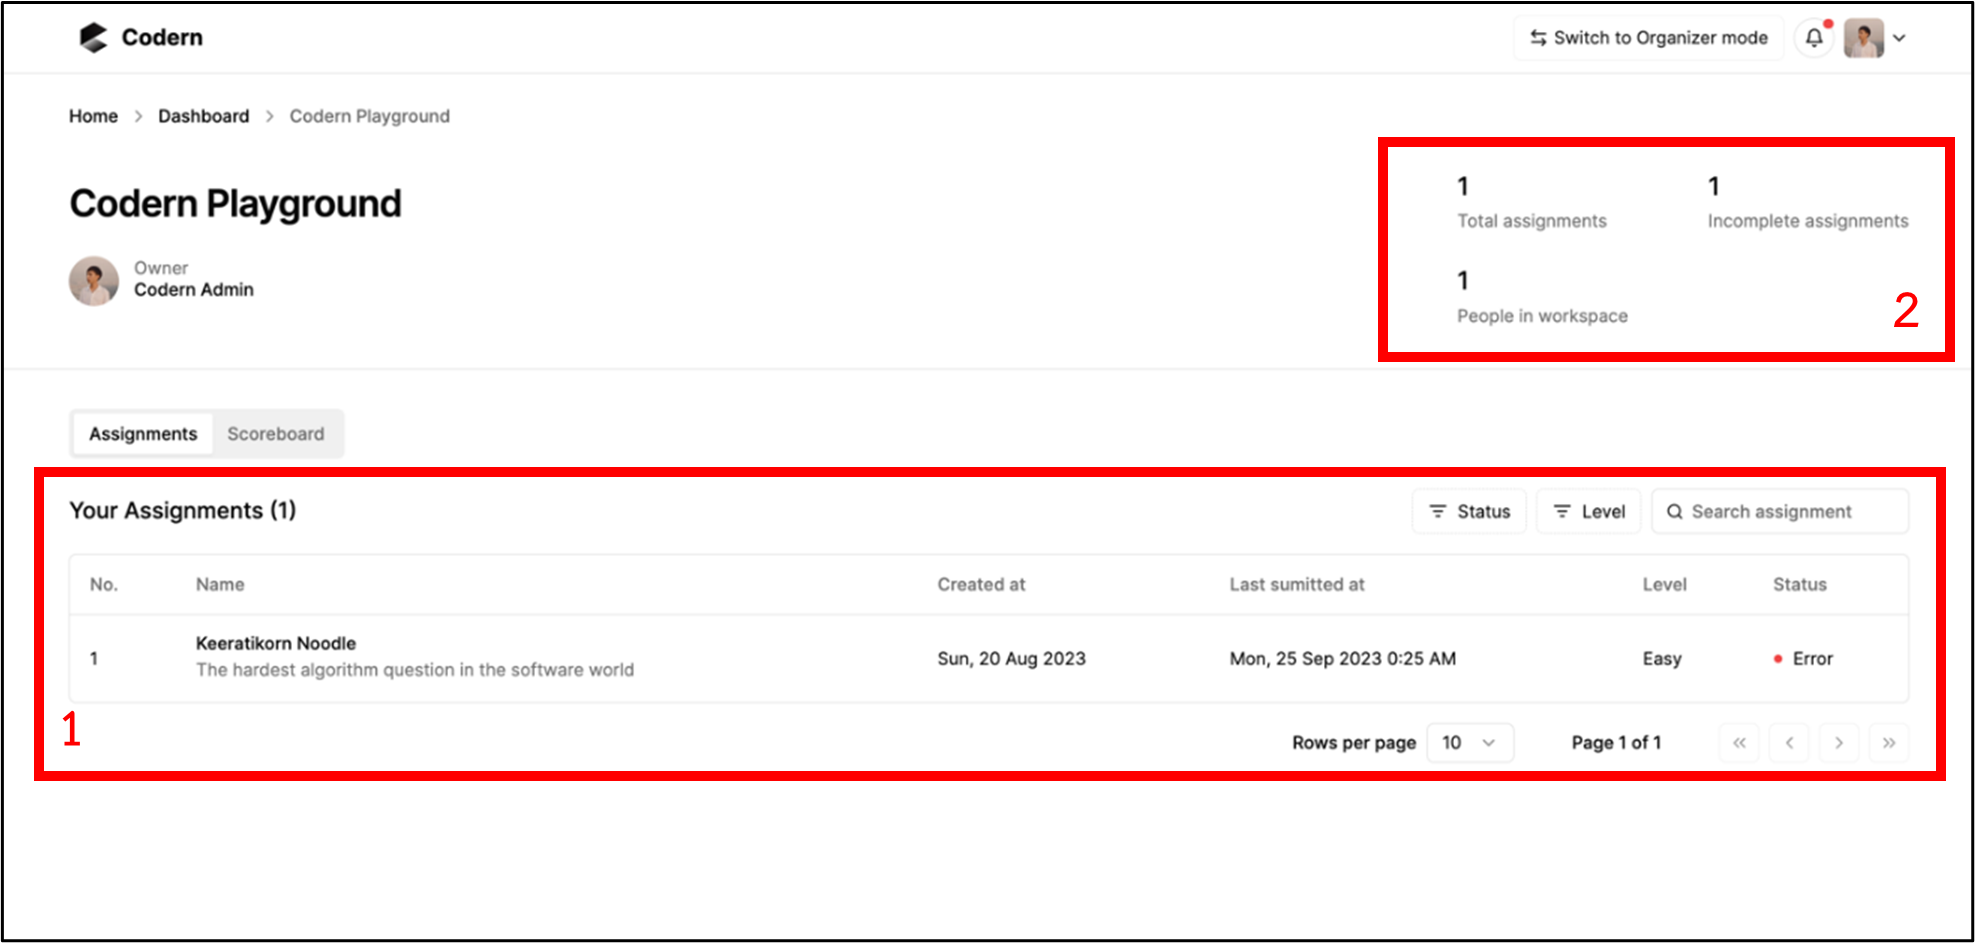
\includegraphics[width=15cm]{figure/ui/ui-assign1.png}
    \caption[ส่วนประสานต่อผู้ใช้ หน้ารายการโจทย์ปัญหา]{ส่วนประสานต่อผู้ใช้ หน้ารายการโจทย์ปัญหา}
    \label{fig:ui-assign1}
  \end{figure}
}

%%%%%%%%%%% ORGANIZER ASSIGNMENT LIST %%%%%%%%%%%
\hypertarget{ui-assign2}{
  \begin{figure}[H]
    \centering
    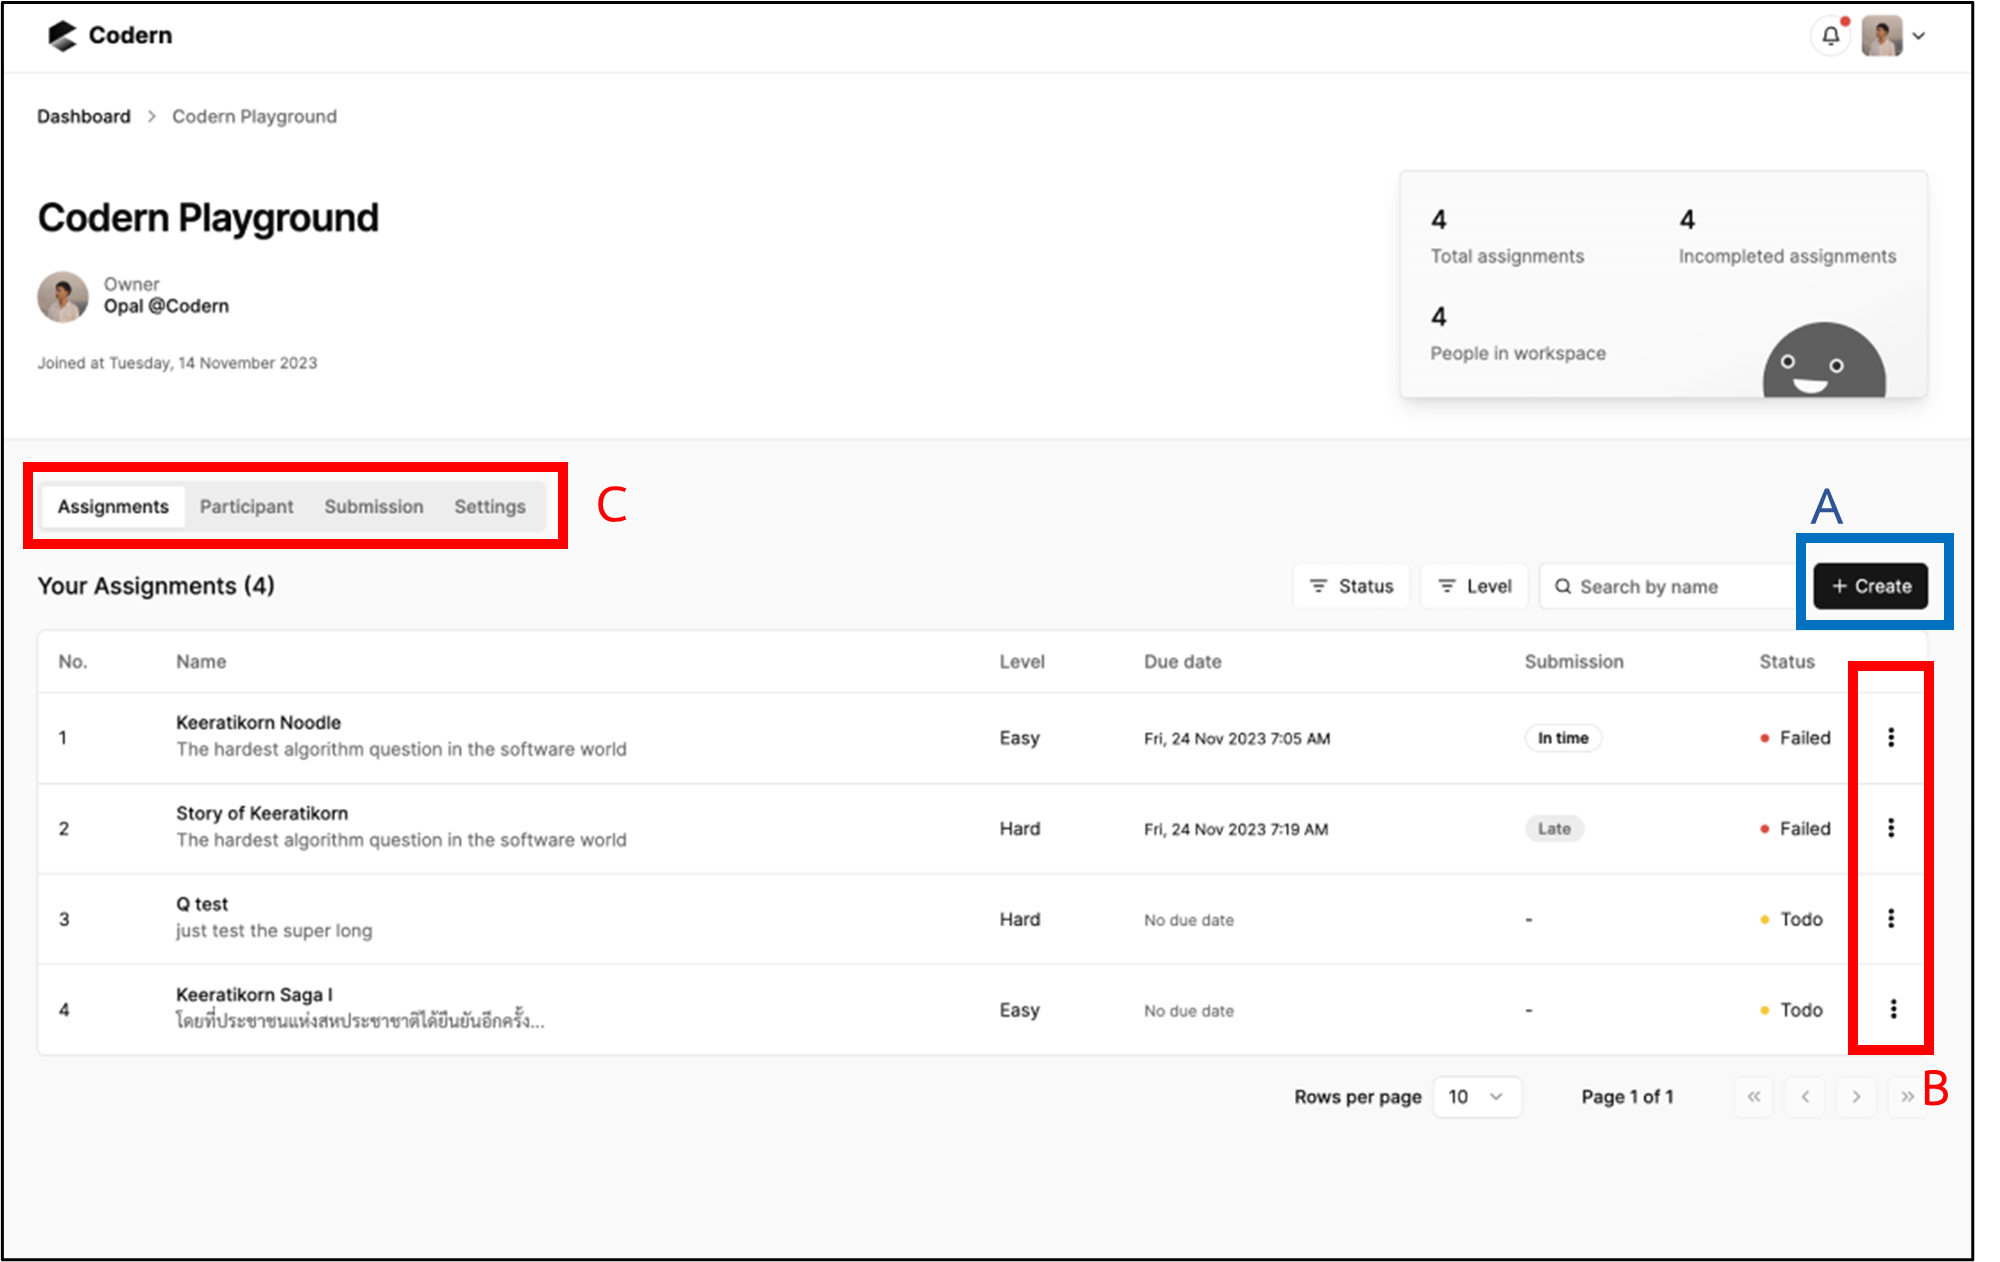
\includegraphics[width=15cm]{figure/ui/ui-assign2.png}
    \caption[ส่วนประสานต่อผู้ใช้ หน้ารายการโจทย์ปัญหาในมุมมองของผู้ดูเเลระบบ]{ส่วนประสานต่อผู้ใช้ หน้ารายการโจทย์ปัญหา ในมุมมองของผู้ดูเเลระบบ}
    \label{fig:ui-assign2}
  \end{figure}
}
\thaijustify{
  ในอีกฝั่ง ในส่วนของผู้ดูแลในรูปที่~\ref{fig:ui-assign2} ก็จะแสดงผลคล้ายคลึงกับฝั่งของผู้ใช้ในรูปที่~\ref{fig:ui-assign1} มีความต่างที่มีปุ่ม “Create Assignment” (กรอบสีน้ำเงิน A) ซึ่งเมื่อกดแล้วจะนำไปสู่รูปที่~\ref{fig:ui-assign3} ซึ่งเป็นฟอร์มสำหรับสร้างการบ้าน โจทย์ปัญหาหรือข้อสอบ สำหรับให้อาจารย์ผู้สอนหรือเจ้าของห้องได้ใช้, ปุ่มรูป "Kebab Menu" ท้ายสุดของแต่ละแถวเพิ่มขึ้นมา (กรอบสีแดง B) ซึ่งเมื่อกดแล้วจะนำพาไปหน้าเเก้ไขโจทย์ปัญหาข้อนั้นๆ ในหน้านั้น (รูปที่~\ref{fig:ui-assign4}) ผู้ดูเเลระบบหรือเจ้าของห้องสามารถแก้ไขข้อมูลของ Assignment นั้น ๆ ได้
}
\thaijustify{
  สามารถใช้แถบปุ่ม Tab (ในกรอบ C) สามารถที่จะย้ายหน้า ไปยังเเถบอื่นได้ แถบดังกล่าวประกอบด้วยหน้า Participants ตามรูปที่~\ref{fig:ui-assign6}, Submission ในรูปที่~\ref{fig:ui-assign7}, Settings ดัง\crefrange{fig:ui-assign-settings1}{fig:ui-assign-settings3}
}
%%%%%%%%%%% CREATE ASSIGNMENT %%%%%%%%%%%
\hypertarget{ui-assign3}{
  \begin{figure}[H]
    \centering
    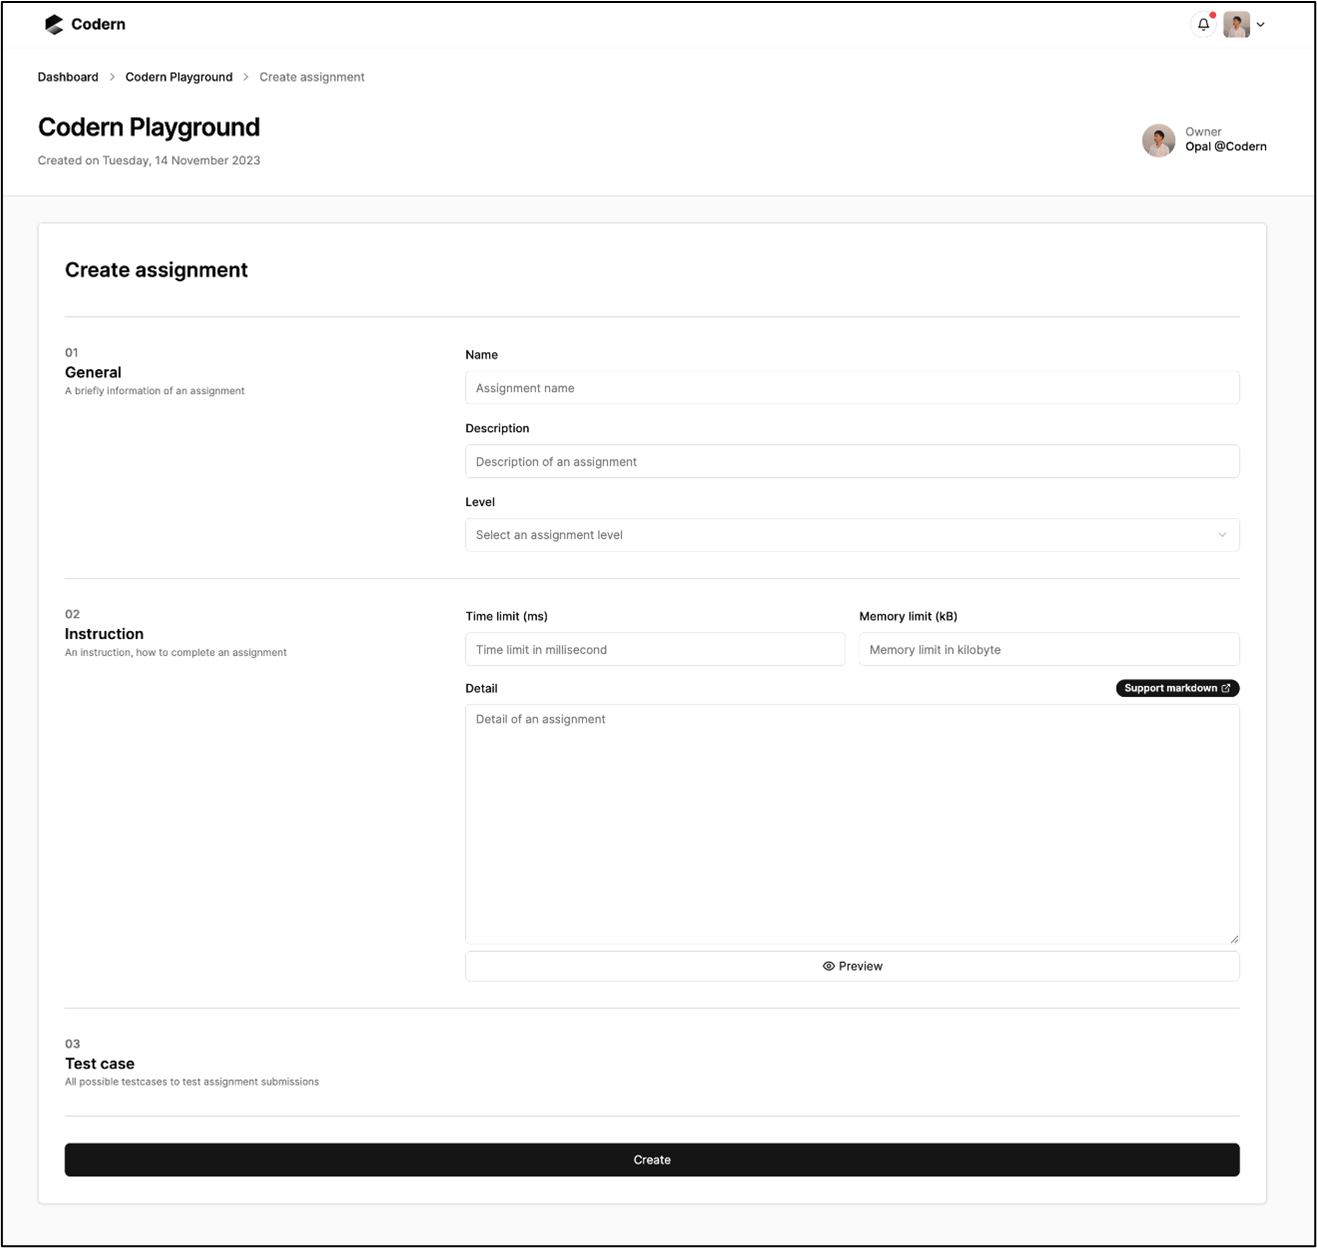
\includegraphics[width=15cm]{figure/ui/ui-assign3.png}
    \caption[ส่วนประสานต่อผู้ใช้ หน้าฟอร์มสร้างโจทย์ปัญหาของผู้ดูเเลระบบ]{ ส่วนประสานต่อผู้ใช้ หน้าฟอร์มสร้างโจทย์ปัญหาของผู้ดูเเลระบบ}
    \label{fig:ui-assign3}
  \end{figure}
}
\hypertarget{ui-assign4}{
  \begin{figure}[H]
    \centering
    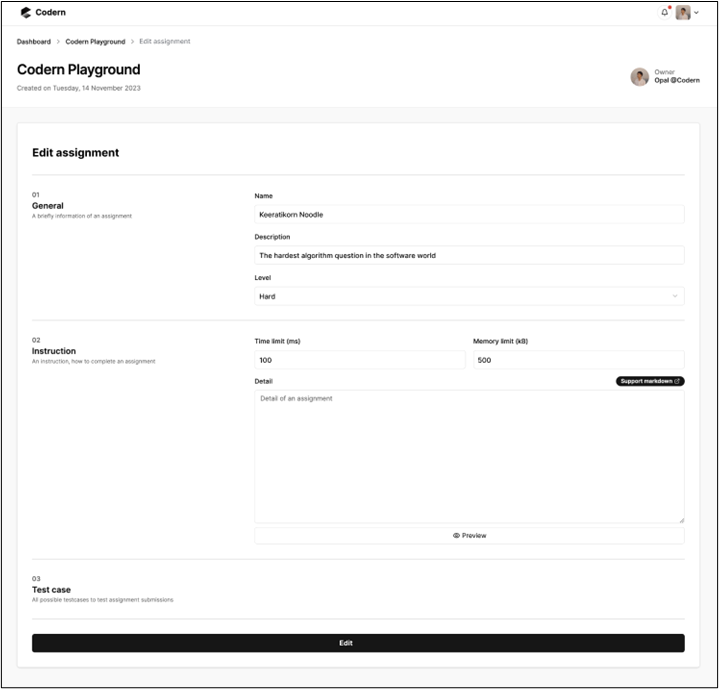
\includegraphics[width=15cm]{figure/ui/ui-assign4.png}
    \caption[ส่วนประสานต่อผู้ใช้ หน้าฟอร์มแก้ไขโจทย์ปัญหาของผู้ดูเเลระบบ]{ ส่วนประสานต่อผู้ใช้ หน้าฟอร์มแก้ไขโจทย์ปัญหาของผู้ดูเเลระบบ}
    \label{fig:ui-assign4}
  \end{figure}
}
\thaijustify{
  ซึ่งภายในรูปที่~\ref{fig:ui-assign3} นั้น อาจารย์หรือผู้ดูแลสามารถเพิ่มโจทย์ปัญหาใหม่เข้าสู่ระบบได้ โดยจะมีข้อมูลของโจทย์ปัญหาให้กรอกตามกำหนด ประกอบไปด้วย ชื่องาน, รายละเอียดงาน, ระดับความยาก, จำนวนหน่วยความจำที่ใช้ได้ (Memory Limit), ระยะเวลาที่ใช้ในการหาคำตอบ (Runtime Limit), รายละเอียดของโจทย์, ตัวอย่างผลลัพธ์ (Test case) และนอกจากนี้ยังสามารถกด Preview เพื่อดูตัวอย่างของโจทย์ที่จะออกมาได้อีกด้วย เมื่อกดปุ่ม "Create" ด้านล่างสุด โจทย์ปัญหาก็จะถูกสร้างขึ้น
}
\thaijustify{
  ส่วนภายในหน้า Edit Assignment ดังรูปที่~\ref{fig:ui-assign4} นั้น จะเป็นหน้าที่อาจารย์หรือผู้ดูแลสามารถแก้ไขข้อมูลของโจทย์ปัญหานั้นๆ ที่ถูกสร้างไว้แล้วได้ โดยจะสามารถแก้ไขข้อมูลได้ทั้งหมด ตั้งแต่ ชื่องาน, รายละเอียดงาน, ระดับความยาก, จำนวนหน่วยความจำที่ใช้ได้(Memory Limit), ระยะเวลาที่ใช้ในการหาคำตอบ (Runtime Limit), รายละเอียดของโจทย์ และตัวอย่างผลลัพธ์ (Test case)
}
\pagebreak
%%%%%%%%%%% ORGANIZER MANAGE USER PARTICIPANTS %%%%%%%%%%%
\hypertarget{ui-assign6}{
  \begin{figure}[H]
    \centering
    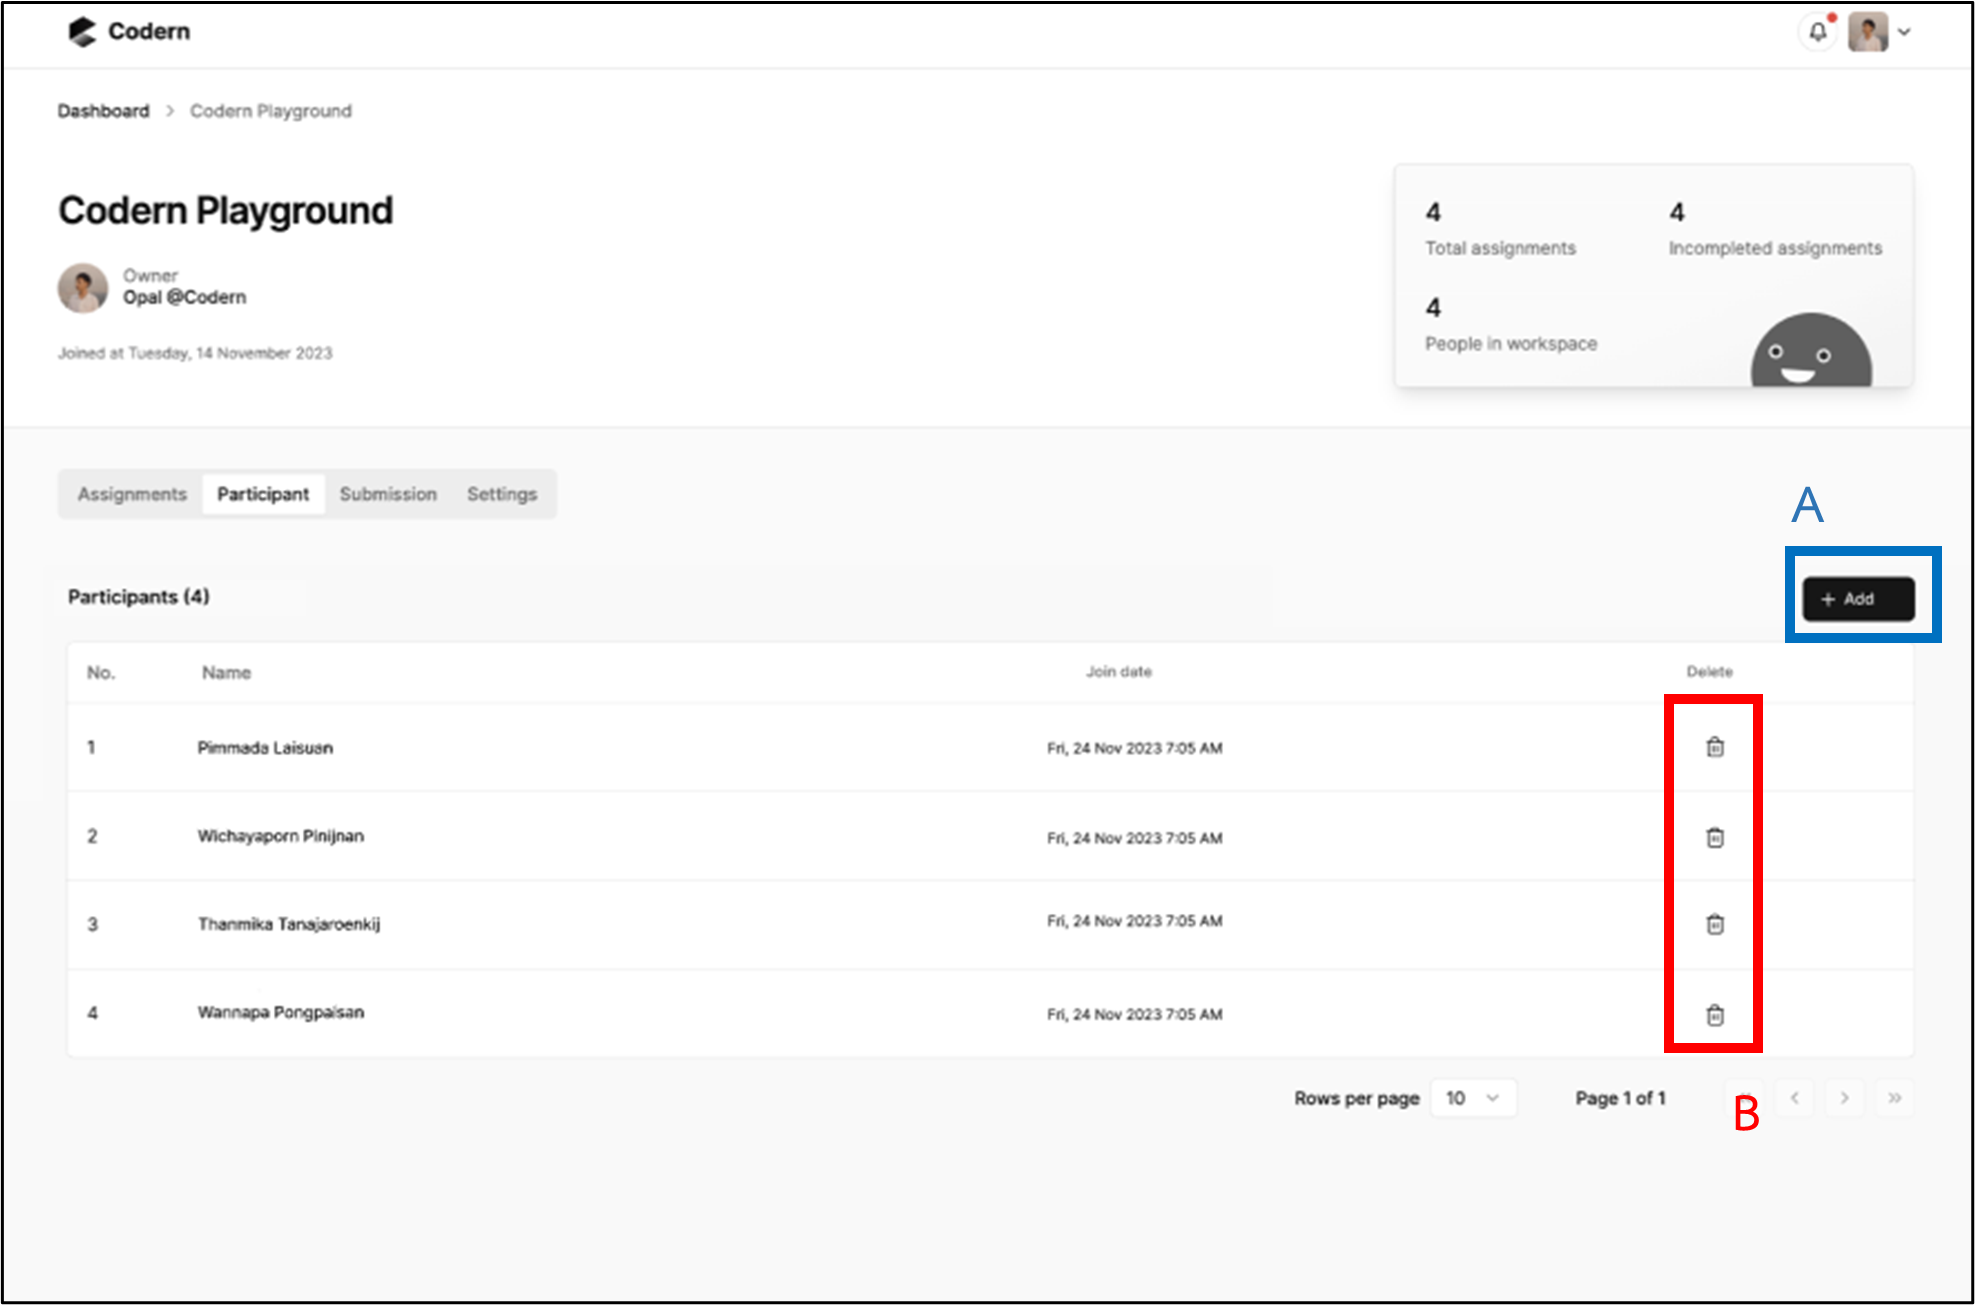
\includegraphics[width=15cm]{figure/ui/ui-assign6.png}
    \caption[ส่วนประสานต่อผู้ใช้ หน้ารายชื่อผู้ใช้ใน Workspace ทั้งหมดในมุมมองของผู้ดูเเลระบบ]{ส่วนประสานต่อผู้ใช้ หน้ารายชื่อผู้ใช้ใน Workspace ทั้งหมด ในมุมมองของผู้ดูเเลระบบ}
    \label{fig:ui-assign6}
  \end{figure}
}
\thaijustify{
  หากกดตรง Tab ตรง "Participant" (ตรงกรอบ C รูปที่~\ref{fig:ui-assign2}) หน้าในรูปที่~\ref{fig:ui-assign6} จะแสดงขึ้นมา โดยหน้าดังกล่าวเป็นหน้าแสดงรายละเอียดสมาชิกของห้องเรียนนั้น ๆ โดยจะแสดงจำนวนสมาชิก รายชื่อนามสกุล วันที่สมาชิกคนนั้น ๆ เข้าร่วมห้องเรียน และผู้ดูเเลระบบจะสามารถลบสมาชิกคนนั้น ๆ ออกจากห้องเรียนได้ด้วยปุ่ม "Delete" ที่ท้ายรายชื่อคนนั้น ๆ (กรอบสีน้ำเงิน A) รวมถึงสามารถเพิ่มสมาชิกใหม่เข้ามาได้ด้วยปุ่ม Add (กรอบสีแดง B) เเต่ถ้าหากเป็นผู้ใช้ธรรมดาทั่วไป จะมองไม่เห็นปุ่ม "Add" หรือปุ่ม "Delete"
}
\pagebreak
%%%%%%%%%%% ORGANIZER MANAGE USER SUBMISSION %%%%%%%%%%%
\hypertarget{ui-assign7}{
  \begin{figure}[H]
    \centering
    \fbox{
      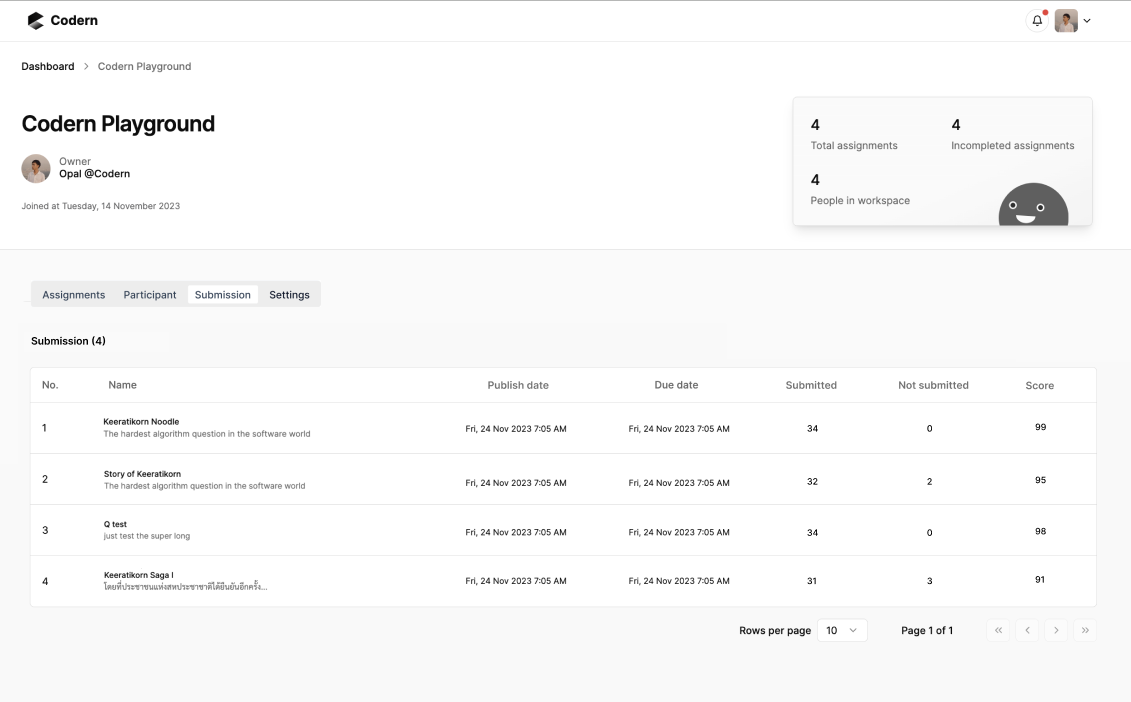
\includegraphics[width=15cm]{figure/ui/ui-assign7.png}
    }
    \caption[ส่วนประสานต่อผู้ใช้ หน้ารายการโปรแกรมที่ผู้ใช้ส่งเข้ามาใน Workspace ในมุมมองของผู้ดูเเลระบบ]{ส่วนประสานต่อผู้ใช้ หน้ารายการโปรแกรมที่ผู้ใช้ส่งเข้ามาใน Workspace ในมุมมองของผู้ดูเเลระบบ}
    \label{fig:ui-assign7}
  \end{figure}
}
\thaijustify{
  ต่อมา เมื่อกดปุ่ม Tab ที่ "Submission" แล้ว จะปรากฏหน้าดังรูปที่~\ref{fig:ui-assign7} โดยหน้าดังกล่าวเป็นหน้าแสดงรายละเอียดรายการโปรแกรมทั้งหมดที่มีของห้องเรียนนั้น ๆ โดยจะแสดงรายชื่อและรายละเอียดของโปรแกรมนั้น ๆ วันที่เผยแพร่โปรแกรมนั้น ๆ วันสุดท้ายที่กำหนดส่งโปรแกรมนั้น ๆ จำนวนคนที่ส่งคำตอบเข้ามาแล้วทั้งหมด จำนวนคนที่ยังไม่ส่งคำตอบเข้ามา และผลคะแนนโดยเฉลี่ยของโปรแกรมข้อนั้น ๆ ผู้ดูเเลระบบจะสามารถกดเข้าไปในชื่อโปรแกรมนั้น ๆ เพื่อดูรายชื่อสมาชิกของห้องเรียนที่ได้ทำการส่งคำตอบเข้ามาแล้วได้ ซึ่งจะปรากฏดังรูปที่~\ref{fig:ui-assign8}
}
\hypertarget{ui-assign8}{
  \begin{figure}[H]
    \centering
    \fbox{
      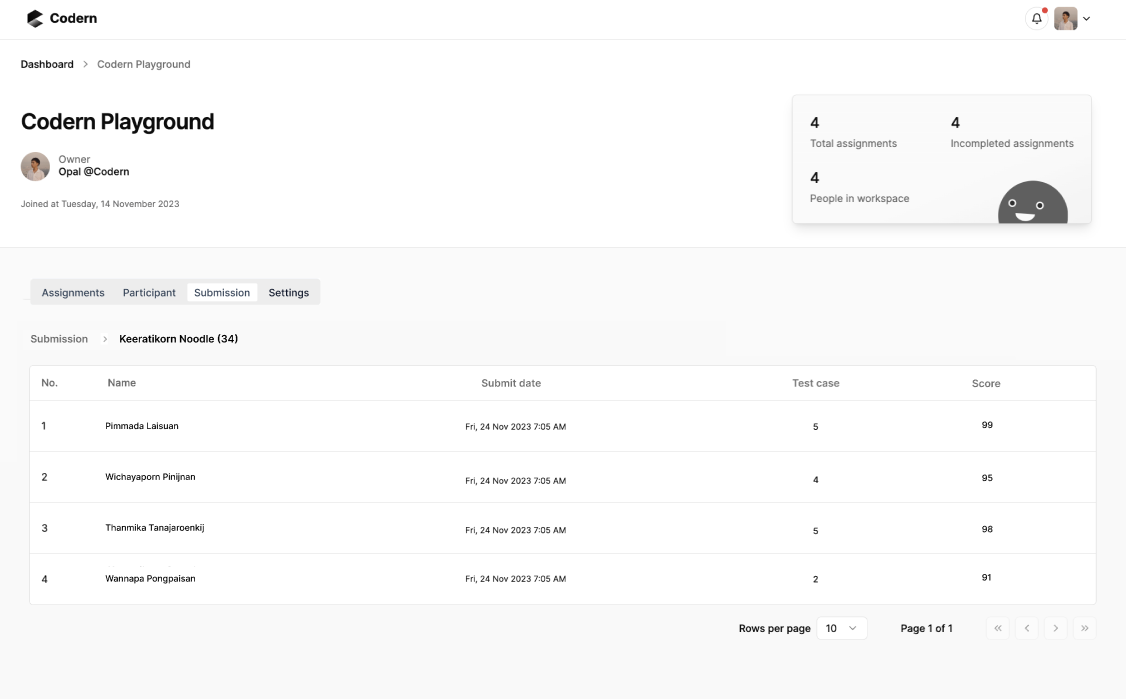
\includegraphics[width=15cm]{figure/ui/ui-assign8.png}
    }
    \caption[ส่วนประสานต่อผู้ใช้ หน้ารายชื่อสมาชิกห้องเรียนที่ได้ส่งคำตอบของโปรแกรมนั้น ๆ ของผู้ดูเเลระบบ]{ส่วนประสานต่อผู้ใช้ หน้ารายชื่อสมาชิกห้องเรียนที่ได้ส่งคำตอบของโปรแกรมนั้น ๆ เข้ามาใน Workspace ของผู้ดูเเลระบบ}
    \label{fig:ui-assign8}
  \end{figure}
}
\thaijustify{
  ภายในหน้าดังกล่าว จะแสดงรายชื่อสมาชิกทั้งหมดที่ได้ทำการส่งคำตอบของโปรแกรมนั้น ๆ เข้ามาใน Workspace แล้วดังรูปที่~\ref{fig:ui-assign8} และจะแสดงรายละเอียดวันเวลาที่ส่งคำตอบเข้ามา จำนวนเทสเคสที่ถูกต้อง และผลคะแนนที่ได้ของโปรแกรมนั้น ๆ ผู้ดูเเลระบบจะสามารถกดเข้าไปในชื่อผู้ใช้คนนั้น ๆ เพื่อดูคำตอบโปรแกรมที่ผู้ใช้คนนั้น ๆ เข้ามาได้ ทั้งผู้ดูแลยังสามารถแสดงความคิดเห็นของตนส่งให้ผู้ใช้คนนั้น ๆ ได้อีกด้วย ซึ่งรายละเอียดหน้าดังกล่าวจะปรากฏดังรูปที่~\ref{fig:ui-code3}
}
\hypertarget{ui-code3}{
  \begin{figure}[H]
    \centering
    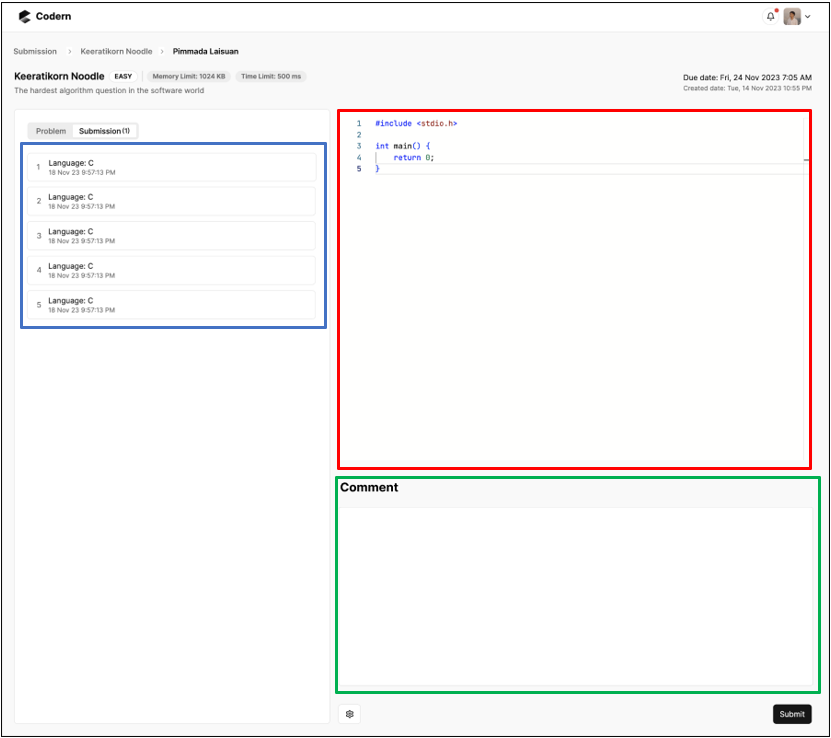
\includegraphics[width=15cm]{figure/ui/ui-code3.png}
    \caption[ส่วนประสานต่อผู้ใช้ หน้าแสดงคำตอบของโปรแกรมที่ผู้ใช้ได้ส่งเข้ามาใน Workspace ของผู้ดูเเลระบบ]{ส่วนประสานต่อผู้ใช้ หน้าแสดงคำตอบของโปรแกรมที่ผู้ใช้ได้ส่งเข้ามาใน Workspace ของผู้ดูเเลระบบ}
    \label{fig:ui-code3}
  \end{figure}
}
\thaijustify{
  หลังจากเข้ามาแล้ว ภายในหน้านี้จะแสดงคำตอบของโปรแกรมที่ผู้ใช้คนนั้น ๆ ได้ส่งเข้ามาใน Workspace ดังรูปที่~\ref{fig:ui-code3} โดยรายละเอียดจะแบ่งได้เป็นสามส่วนหลักคือ รายการคำตอบโปรแกรมของแต่ละเทสเคสที่ผู้ใช้ได้ส่งเข้ามา (ตรงกรอบสีน้ำเงินทางซ้ายมือรูปที่~\ref{fig:ui-code3}) เมื่อกดที่รายการคำตอบแล้ว จะแสดงคำตอบโปรแกรมของรายการนั้น ๆ ในกล่อง (ตรงกรอบสีแดงทางขวาบนรูปที่~\ref{fig:ui-code3}) และทางด้านขวาล่างจะมีพื้นที่สำหรับให้ผู้ดูแลแสดงความคิดเห็นของตน (ตรงกรอบสีเขียวทางขวาล่างรูปที่~\ref{fig:ui-code3}) ซึ่งเมื่อกดปุ่ม "Submit" ทางขวาล่างสุดแล้ว ความคิดเห็นก็จะถูกส่งไปยังผู้ใช้คนนั้น ๆ
}
%%%%%%%%%%% ASSIGN SETTINGS %%%%%%%%%%%
\hypertarget{ui-assign-settings1}{
  \begin{figure}[H]
    \centering
    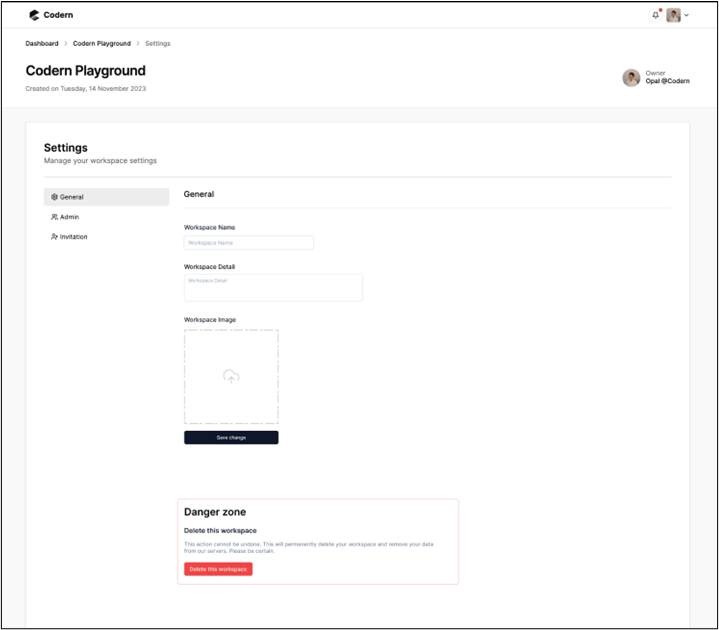
\includegraphics[width=15cm]{figure/ui/ui-assign-settings1.png}
    \caption[ส่วนประสานต่อผู้ใช้ หน้าตั้งค่า Workspace ใน Section "General" ในมุมมองของผู้ดูเเลระบบ]{ส่วนประสานต่อผู้ใช้ หน้าตั้งค่า Workspace ใน Section "General" ในมุมมองของผู้ดูเเลระบบ}
    \label{fig:ui-assign-settings1}
  \end{figure}
}
\thaijustify{
  หลังจากกดตรง Tab ตรง "Settings" (ตรงกรอบ C รูปที่~\ref{fig:ui-assign2} ซึ่งมีเเต่ผู้ดูเเลระบบเท่านั้นที่จะเห็น) หน้าในรูปที่~\ref{fig:ui-assign-settings1} จะปรากฎขึ้นมา ซึ่งหน้าข้างต้นเป็นหน้าสำหรับตั้งค่าข้อมูลต่าง ๆ ภายในห้องเรียนหรือกลุ่มเรียนนั้น ๆ ซึ่งมีเฉพาะผู้ดูเเลเท่านั้นที่จะสามารถเข้าไปดูเเละเเก้ไขได้เท่านั้น โดยจะแบ่งเป็น 3 ส่วนย่อย ประกอบไปด้วย General settings ซึ่งจะเป็นเมนูแรกสุดดังรูปที่~\ref{fig:ui-assign-settings1} ตามมาด้วย Admin settings และ Invitation settings ดังรูปที่~\ref{fig:ui-assign-settings2} และรูปที่~\ref{fig:ui-assign-settings3} ตามลำดับ
}
\thaijustify{
  โดย "General settings" ดังรูปที่~\ref{fig:ui-assign-settings1} จะเป็นหน้าสำหรับการแก้ไขข้อมูลทั่วไปของห้องเรียนนั้น ๆ เช่น ชื่อของห้องเรียน หรือ รูปรูปที่แสดง และที่สำคัญยังสามารถลบห้องเรียนนั้น ๆ ได้เมื่อกดที่ปุ่ม Delete this workspace ภายใน Danger zone ซึ่งการลบห้องเรียนนั้นจะเป็นการลบอย่างถาวร ข้อมูลทั้งหมดจะถูกลบโดยไม่สามารถกู้คืนได้อีก
}
%%%%%%%%%%% ASSIGN SETTINGS - ADMIN %%%%%%%%%%%
\hypertarget{ui-assign-settings2}{
  \begin{figure}[H]
    \centering
    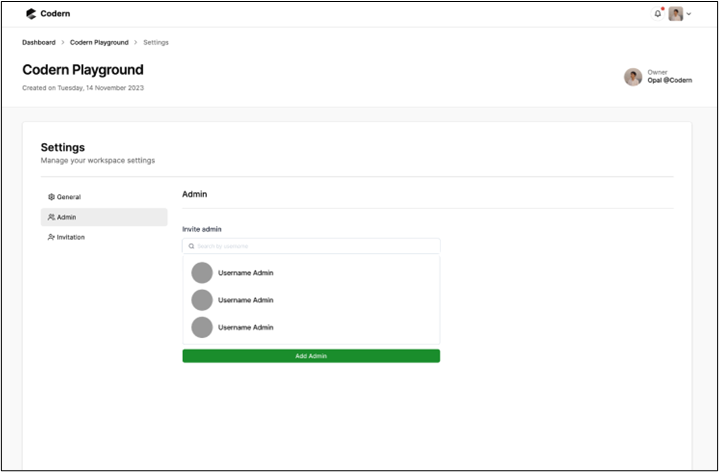
\includegraphics[width=15cm]{figure/ui/ui-assign-settings2.png}
    \caption[ส่วนประสานต่อผู้ใช้ หน้าตั้งค่า Workspace ใน Section "Admin" ในมุมมองของผู้ดูเเลระบบ]{ส่วนประสานต่อผู้ใช้ หน้าตั้งค่า Workspace ใน Section "Admin" ในมุมมองของผู้ดูเเลระบบ}
    \label{fig:ui-assign-settings2}
  \end{figure}
}
\thaijustify{
  ในของ "Admin Settings" ดังรูปที่~\ref{fig:ui-assign-settings2} จะเป็นหน้าสำหรับการเพิ่มแอดมินหรือผู้ดูแลเข้าสู่ห้องเรียนนั้น ๆ โดยจะประกอบด้วยกล่องค้นหา หากค้นหาพบคนที่ต้องการแล้ว เมื่อกดปุ่ม "Add admin" จะเป็นการเพิ่มผู้ดูแลคนนั้น ๆ เข้าสู่ห้องเรียน
}
%%%%%%%%%%% ASSIGN SETTINGS - INVITATION %%%%%%%%%%%
\hypertarget{ui-assign-settings3}{
  \begin{figure}[H]
    \centering
    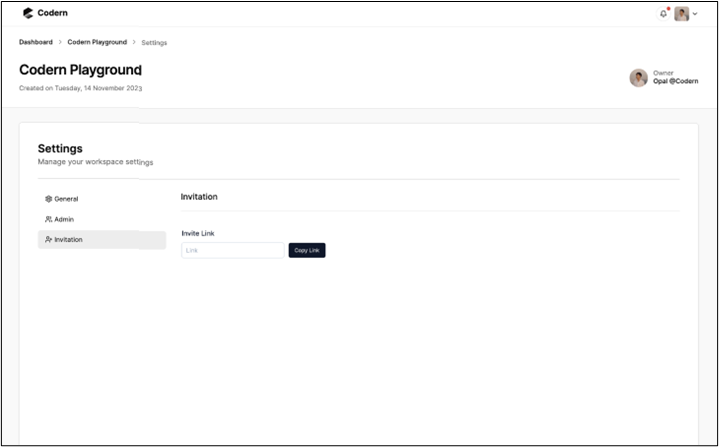
\includegraphics[width=15cm]{figure/ui/ui-assign-settings3.png}
    \caption[ ส่วนประสานต่อผู้ใช้ หน้าตั้งค่า Workspace ใน Section "Invitation" ในมุมมองของผู้ดูเเลระบบ]{ ส่วนประสานต่อผู้ใช้ หน้าตั้งค่า Workspace ใน Section "Invitation" ในมุมมองของผู้ดูเเลระบบ}
    \label{fig:ui-assign-settings3}
  \end{figure}
}
\thaijustify{
  สุดท้ายในส่วนของ "Invitation" Settings ดังรูปที่~\ref{fig:ui-assign-settings3} เป็นหน้าสำหรับการเชิญผู้ใช้ทั่วไปเข้าสู่ห้องเรียนนั้น ๆ โดยตัวผู้ดูแล ซึ่งทำได้โดยจะมีการสร้างรหัสเชิญขึ้น หากกดปุ่ม "Copy link" จะเป็นการคัดลอกรหัสเชิญไปยังคลิปบอร์ด และเมื่อผู้ใช้กรอกรหัสดังกล่าวลงในกล่อง "Join with code" ในรูปที่~\ref{fig:ui-dashboard4} และกดปุ่ม "Join" จะเป็นการเข้าร่วมห้องเรียนนั้น ๆ
}
%%%%%%%%%%% CODE PAGE - PROBLEM %%%%%%%%%%
\thaijustify{
  ถ้าหากกดรายการการบ้าน โจทย์ปัญหา มาสักรายการ (ในรูปที่~\ref{fig:ui-assign1}) ก็จะนำพามาสู่หน้าโจทย์ปัญหาในรูปที่~\ref{fig:ui-code1} โดยในหน้านี้ในโซนที่ 1 จะเป็นช่องแผงเขียนโปรแกรม สามารถที่จะเขียนโปรแกรมภาษาคอมพิวเตอร์ในโซนนี้ได้ ในโซนที่ 2 จะเป็นแสดงรายละเอียดของโจทย์ตั้งแต่เนื้อหาโจทย์ ไปจนถึงจำนวนหน่วยความจำที่ใช้ได้ (Memory Limit) และระยะเวลาที่ใช้ในการหาคำตอบ (Runtime Limit) ถ้าหากต้องการส่งก็สามารถที่จะกดปุ่ม “Submit” ที่กรอบน้ำเงิน A เพื่อส่งงานเขียนโปรแกรมไปให้ตรวจ และอีกทั้งก่อนส่ง ก็ยังสามารถที่จะตั้งค่าและเลือก Compiler ที่ต้องการจะใช้ในการตรวจงานเขียนโปรแกรมดังกล่าวได้ที่ Dropdown ที่กรอบน้ำเงิน B หลังจากผู้ใช้กดส่งไปตรวจแล้ว สามารถติดตามผลได้ในรายการ Submission ซึ่งสามารถกดดูได้ตรงกรอบสีเขียว C ในรูปที่~\ref{fig:ui-code1}
}
\hypertarget{ui-code1}{
  \begin{figure}[H]
    \centering
    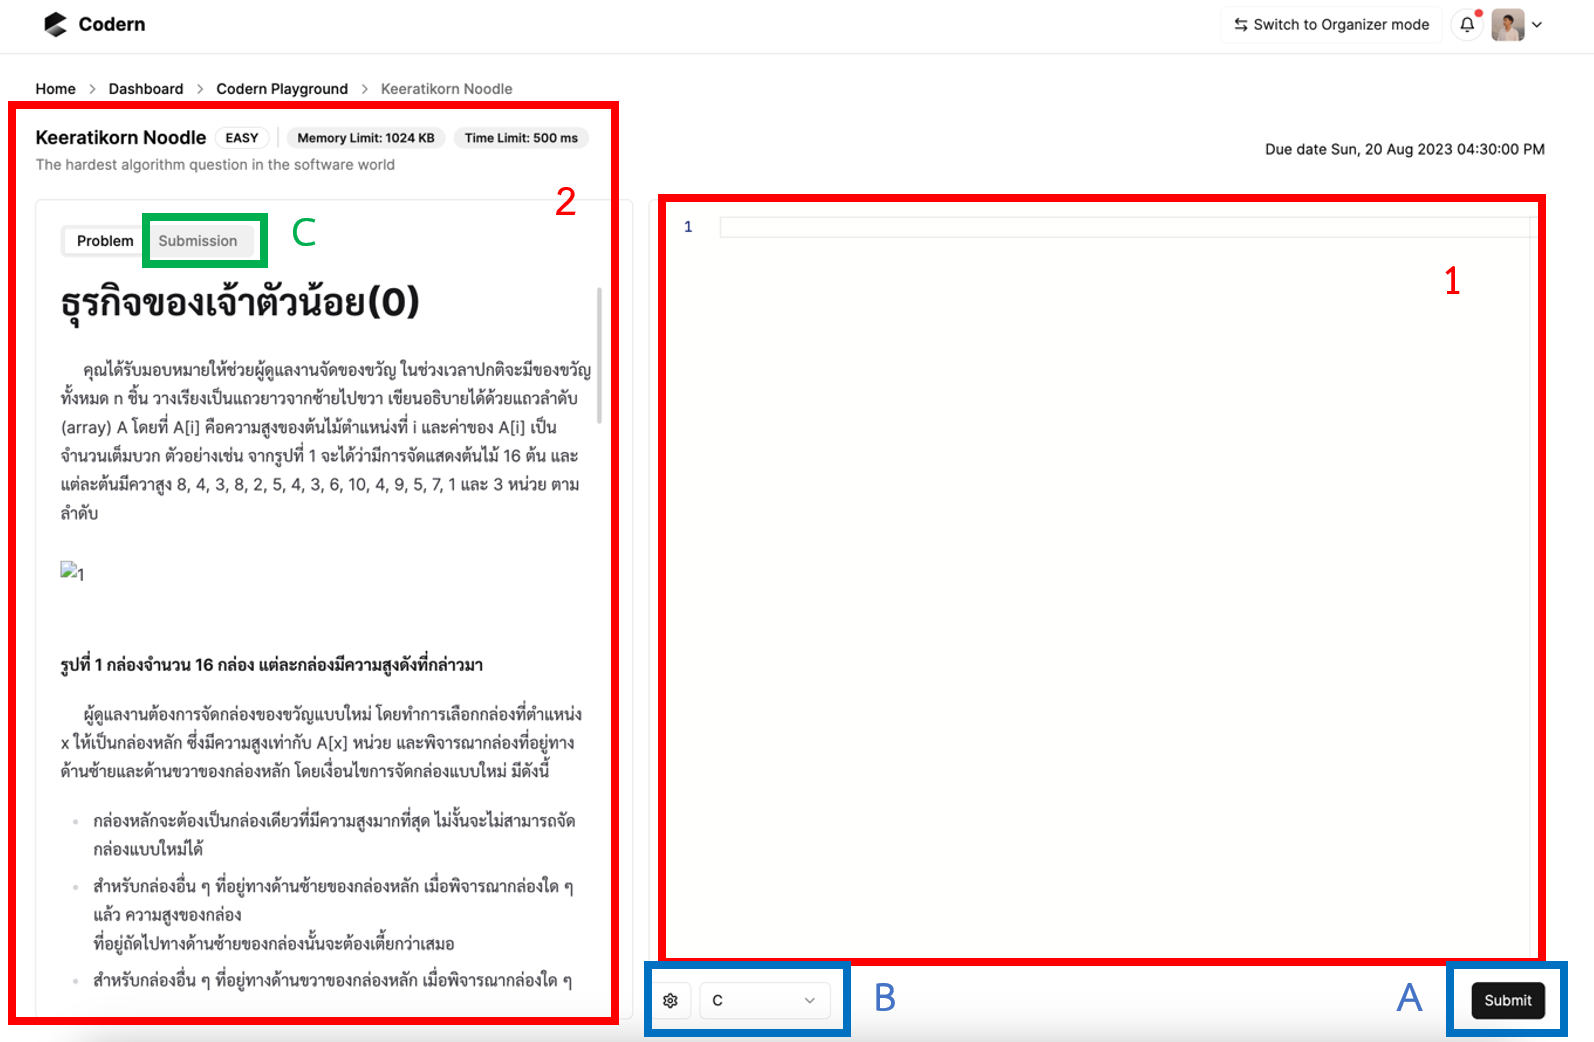
\includegraphics[width=15cm]{figure/ui/ui-code1.png}
    \caption[ส่วนประสานต่อผู้ใช้ หน้าโจทย์ปัญหาและแผงเขียนโปรแกรม]{ส่วนประสานต่อผู้ใช้ หน้าโจทย์ปัญหาและแผงเขียนโปรแกรม}
    \label{fig:ui-code1}
  \end{figure}
}
\thaijustify{
  หลังจากกดเลือก Tab ชื่อ "Submission" แผงแสดงผลเนื้อหาโจทย์ จะถูกเปลี่ยนมาเป็นรายการผลส่งการตรวจทั้งหมด ในโซนกรอบแดงที่ 1 ในรูป~\ref{fig:ui-code2} โดยในรายการก็จะแสดงรายละเอียดการส่งแต่ละครั้งที่ผู้ใช้ส่ง มีรายละเอียดต่าง ๆ อาทิเช่น ภาษาที่ส่งไปตรวจ และผลการตรวจของแต่ละ Test Case (ถ้า PASS แปลว่า output ของโปรแกรมที่เขียนให้ผลตรงตาม Test Case ที่โจทย์ข้อนี้ตั้งไว้, แต่ถ้า FAIL ก็จะแสดงว่า output ของโปรแกรมที่เขียนไม่ได้ให้ผลตรงตาม Test Case ที่โจทย์ข้อนี้ตั้งไว้)
}
\hypertarget{ui-code2}{
  \begin{figure}[H]
    \centering
    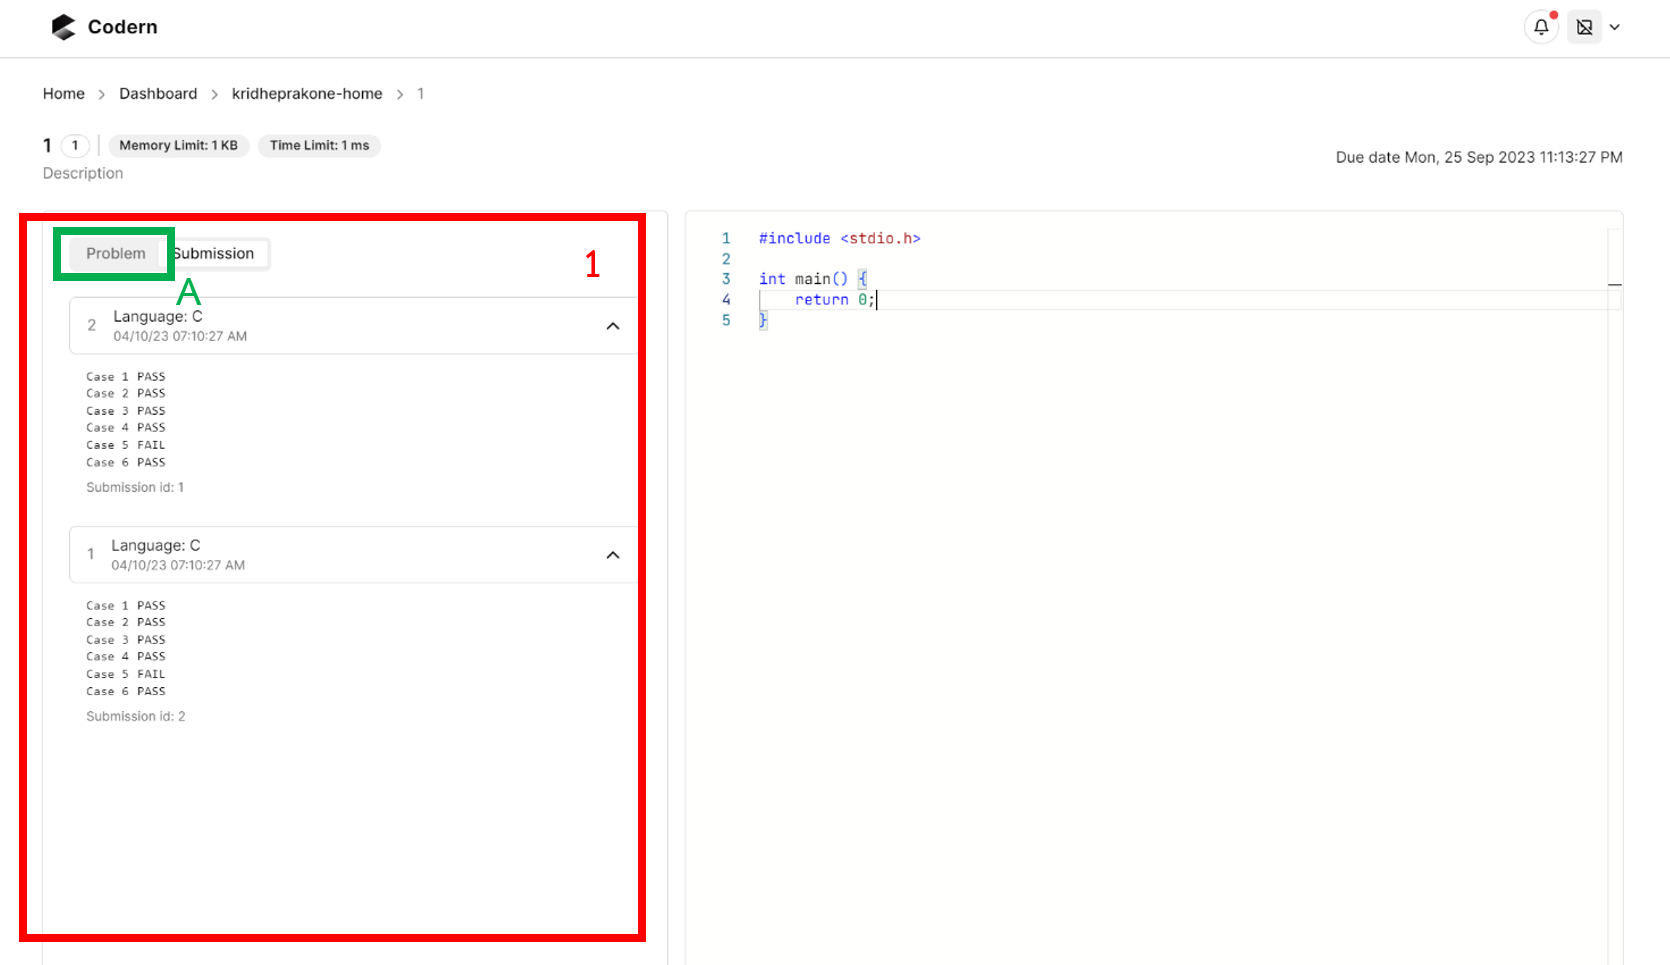
\includegraphics[width=15cm]{figure/ui/ui-code2.png}
    \caption[ส่วนประสานงานต่อผู้ใช้ หน้าโจทย์ปัญหาและแผงเขียนโปรแกรม พร้อมรายการส่งเเละผลการตรวจทั้งหมด]{ส่วนประสานงานต่อผู้ใช้ หน้าโจทย์ปัญหาและแผงเขียนโปรแกรม พร้อมรายการส่งเเละผลการตรวจทั้งหมด}
    \label{fig:ui-code2}
  \end{figure}
}
%%%%%%%%%%% USER ARCHIVE %%%%%%%%%%%
\hypertarget{ui-archive1}{
  \begin{figure}[H]
    \centering
    % \fbox{
    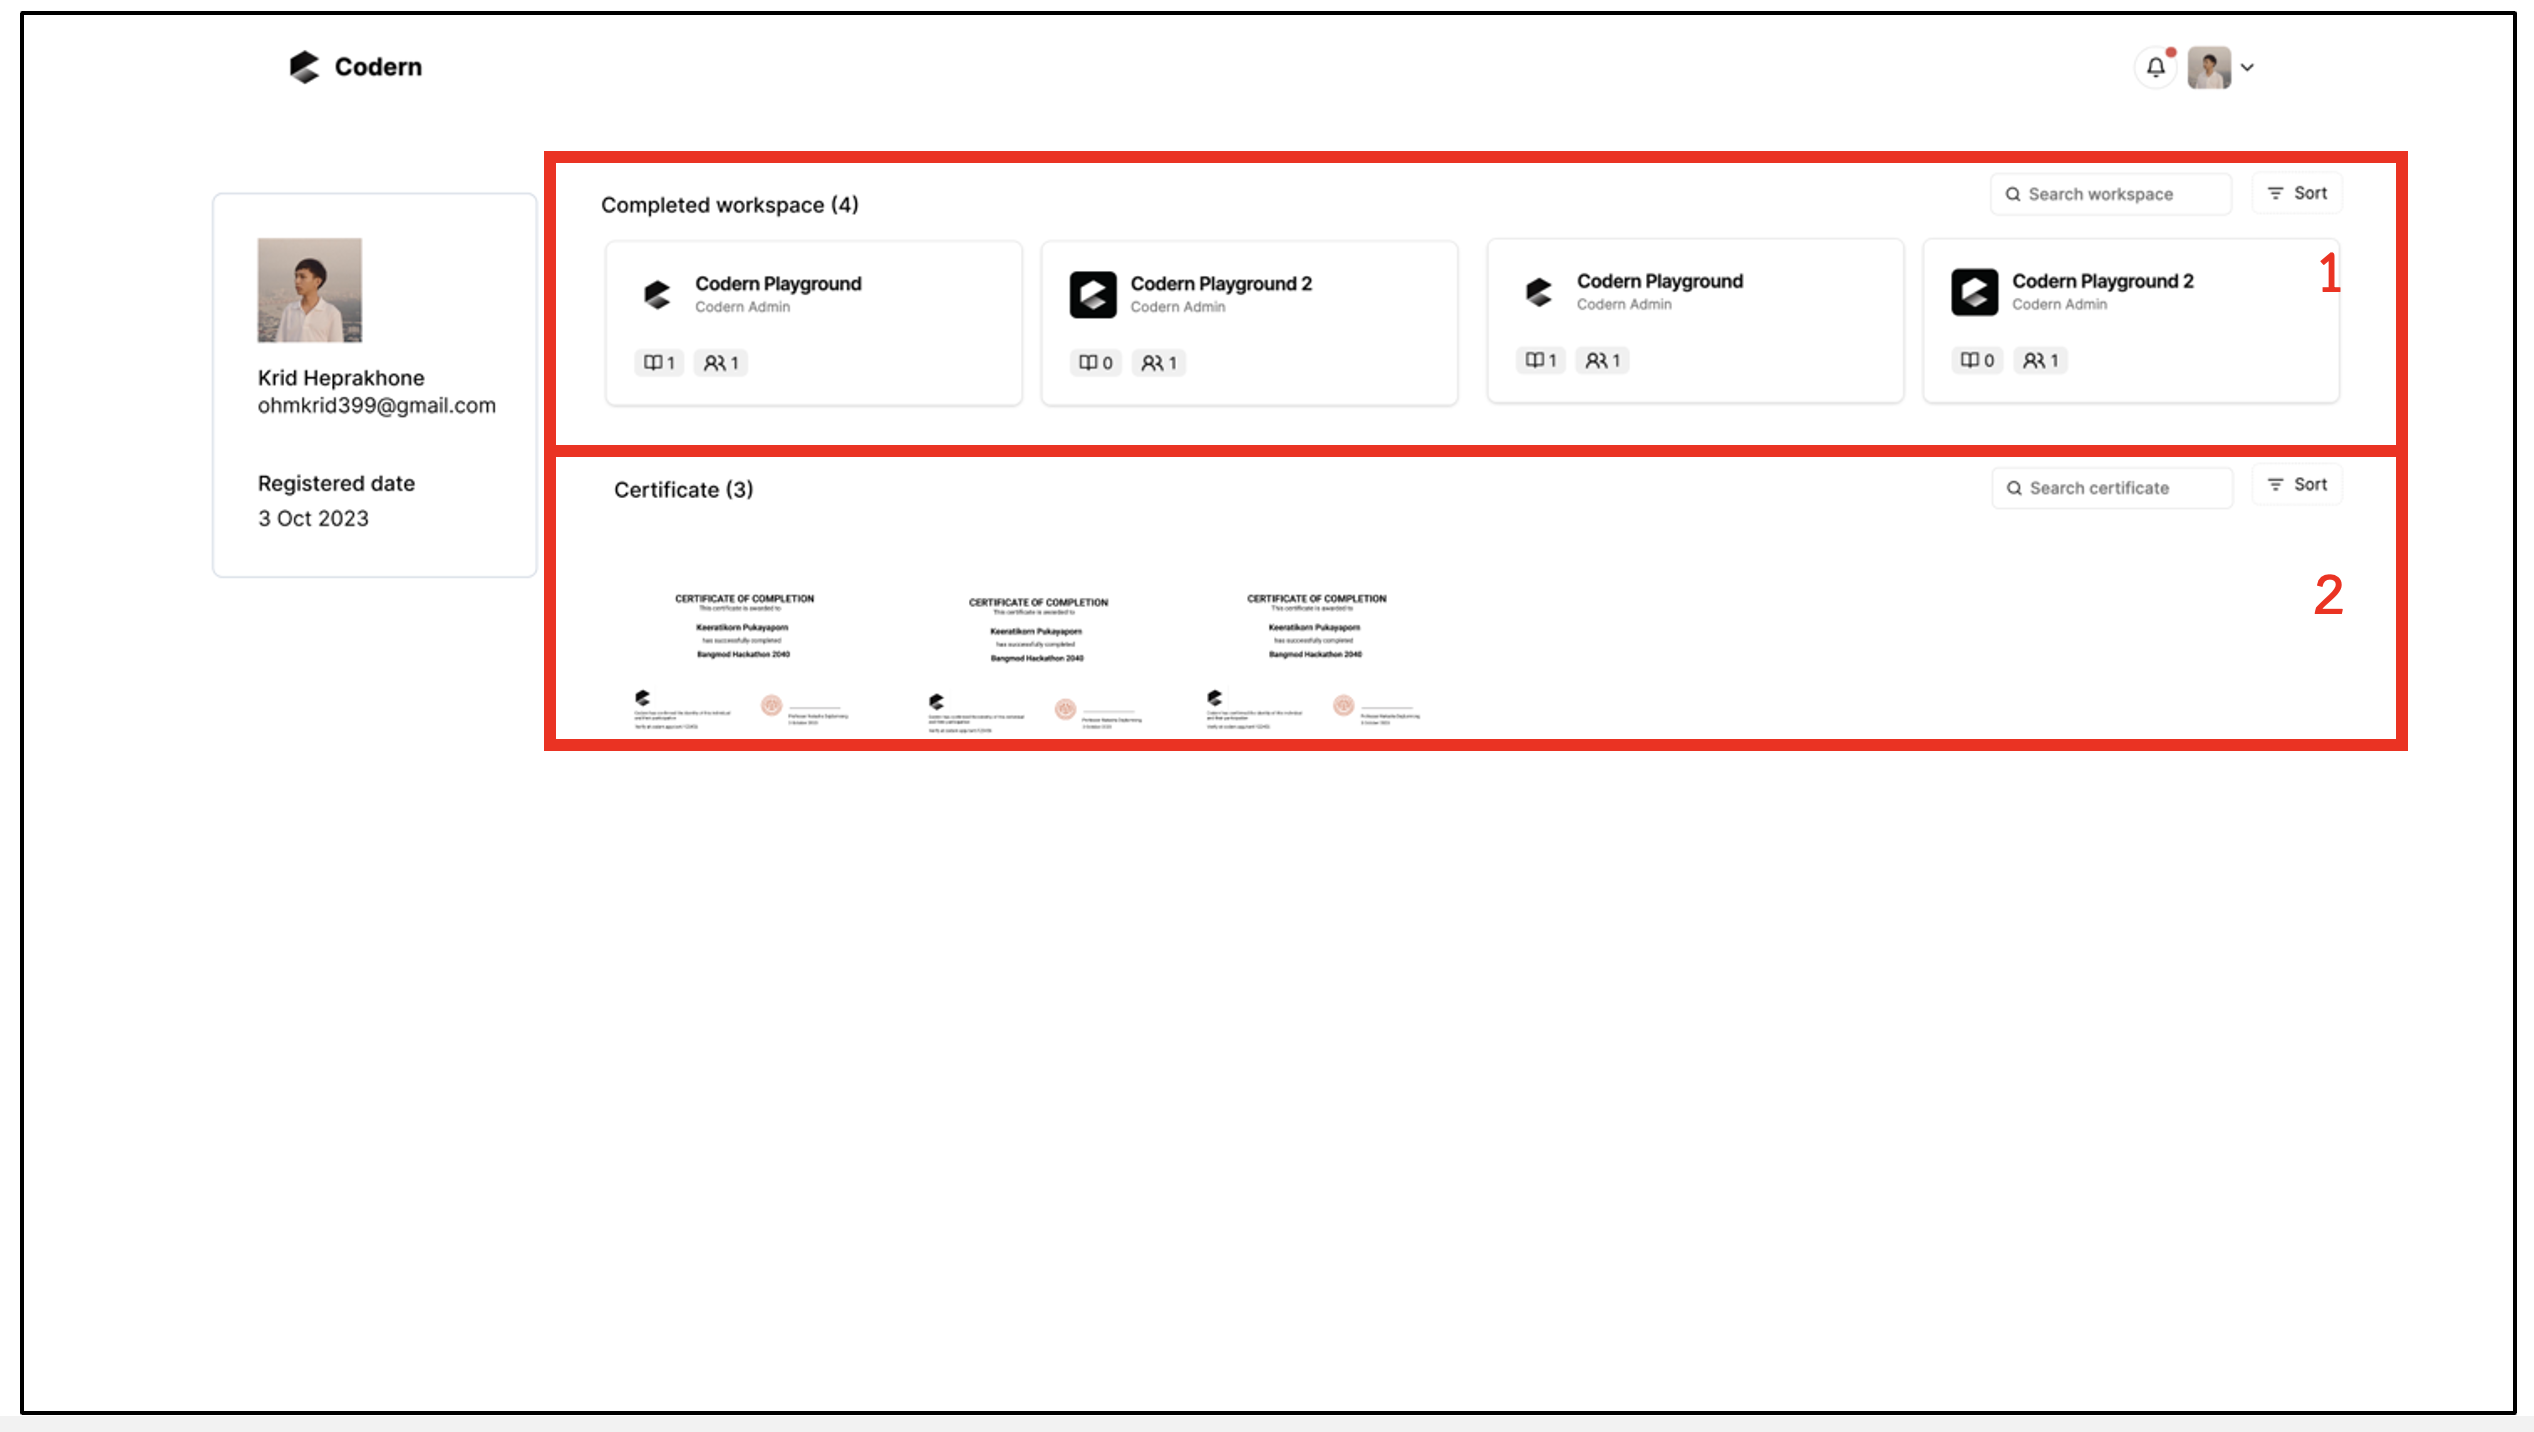
\includegraphics[width=15cm]{figure/ui/ui-archive1.png}
    % }
    \caption[ส่วนประสานงานต่อผู้ใช้ หน้าแสดงข้อมูลของผู้ใช้เก่า]{ส่วนประสานงานต่อผู้ใช้ หน้าแสดงข้อมูล ประวัติการใช้งาน และเกียรติบัตรทั้งหมด ของผู้ใช้เก่า}
    \label{fig:ui-archive1}
  \end{figure}
}
\thaijustify{
  ในอีกโดเมนเเยกจากระบบหลัก (ดูแผนผังการนำทางระหว่างหน้าของเว็บไซต์ ในรูปที่~\ref{fig:nav-map}) หน้าแสดงข้อมูลและประวัติการใช้งานของผู้ใช้เก่า (ในรูปที่~\ref{fig:ui-archive1}) เช่น นักเรียนหรือนักศึกษาที่ได้จบการศึกษาไปแล้ว เป็นต้น
}
\thaijustify{
  ผู้ใช้ทั่วไป (ไม่จำเป็นต้องมีบัญชีบนซอฟต์แวร์ ณ เวลานั้น) สามารถที่จะเข้ามาค้นดูประวัติ ข้อมูลการใช้งาน โจทย์ที่ได้ทำ ห้องหรือกลุ่มเรียนที่เคยได้เข้าร่วม (โซนกรอบแดงที่ 1) พร้อมทั้งค้นเอาเกียรติบัตร (โซนกรอบแดงที่ 2) ไปพิมพ์ใช้งานต่อได้ (เกียรติบัตรจะถูกสร้างขึ้นแก่ผู้ใช้ทุกคนก็ต่อเมื่อเจ้าของห้อง ปิดห้องหรือกลุ่มเรียน) สำหรับยื่นหรือให้การศึกษาต่อ ใช้สมัครงานต่อไปก็ได้
}
\pagebreak
\section{โครงสร้างฐานข้อมูล}
\thaijustify{
  จากรูปที่~\ref{fig:database} ด้านล่าง เป็นแผนภาพแสดงฐานข้อมูลของซอฟต์แวร์ที่ทางคณะผู้จัดทำได้ออกแบบไว้เบื้องต้น ฐานข้อมูลดังกล่าวเป็นแบบ RDMS หรือ Relation Database Management System ที่จะเก็บข้อมูลบนซอฟต์แวร์ตั้งแต่ข้อมูลผู้ใช้ จนไปถึงข้อมูลกลุ่มห้อง/ห้องเรียน ข้อมูลโจทย์ ทั้งเนื้อหาของโจทย์พร้อมทั้งกรณีทดสอบ (หรือ Testcase) ของโจทย์แต่ละข้อ
}
%% Database Struct
\hypertarget{database}{
  \begin{figure}[H]
    \centering
    % \fbox{
    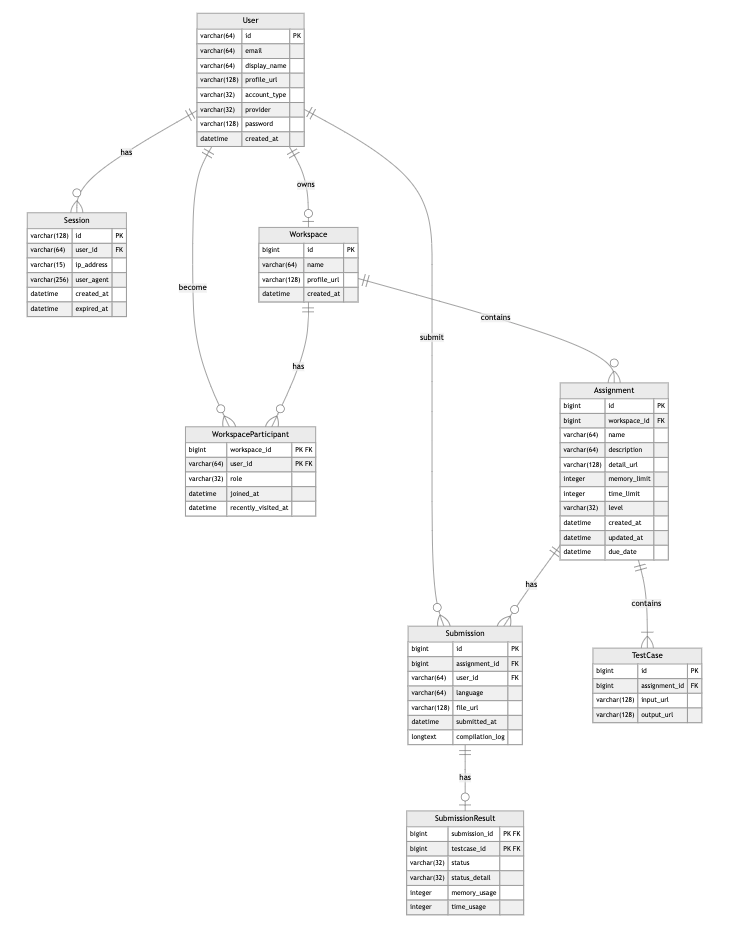
\includegraphics[width=15cm]{figure/diagram/database-v3.png}
    % }
    \caption[แผนภาพฐานข้อมูล]{แผนภาพฐานข้อมูล วาดด้วย \href{https://mermaid.js.org/}{Mermaid JS}}
    \label{fig:database}
  \end{figure}
}
\pagebreak
\subsection{คำบรรยายโครงสร้างฐานข้อมูล}
\thaijustify{
  ในส่วนนี้ ทางกลุ่มเราจะอธิบาย รายละเอียดของแต่ละตารางในระบบฐานข้อมูลนี้ที่ทางกลุ่มได้ออกแบบมาในรูปที่~\ref{fig:database} พร้อมทั้งบรรยายถึงความสัมพันธ์ของตารางนั้น ๆ ที่มีต่อตารางข้อมูลตารางอื่น ๆ
}
\begin{enumerate}
  %% User's Relations
  \item \textbf{User}
        เป็นตารางที่เก็บข้อมูลของผู้ใช้แต่ละคน เช่นอีเมลล์, ชื่อ-นามสกุลขของผู้ใช้ เป็นต้น จากความสัมพันธ์ของตารางดังกล่าว กับตารางอื่น ๆ สามารถสรุปความสัมพันธ์ได้ดังนี้
        \begin{figure}[H]
          \centering
          \subfloat[แผนผังแสดงความสัมพันธ์ระหว่างตาราง User และ Session]{
            \begin{tikzpicture}[auto,node distance=0.7cm]
              % First Entity
              \node[entity] (node1) {User};
              % [grow=up,sibling distance=3cm]
              % child {node[attribute] {Attribute 1}}
              % child {node[attribute] {Attribute 2}}
              % child[grow=left,level distance=3cm] {node[attribute] {Attribute 3}};
              % Relationship
              \node[relationship] (rel1) [right = of node1] {has};
              % Second Entity
              \node[entity] (node2) [right = of rel1]	{Session};
              % Draw an edge between rel1 and node1; rel1 and node2
              \path (rel1) edge node {\(1\)-\(1\)}
              (node1) edge node {\(1\)-\(m\)}	(node2);
            \end{tikzpicture}
            \label{fig:db-user-session}
          } \hspace{0.5cm}
          \subfloat[แผนผังแสดงความสัมพันธ์ระหว่างตาราง User และ Workspace]{
            \begin{tikzpicture}[auto,node distance=0.7cm]
              % First Entity
              \node[entity] (node1) {User};
              % Relationship
              \node[relationship] (rel1) [right = of node1] {owns};
              % Second Entity
              \node[entity] (node2) [right = of rel1]	{Workspace};
              % Draw an edge between rel1 and node1; rel1 and node2
              \path (rel1) edge node {\(1\)-\(1\)}
              (node1) edge node {\(0\)-\(m\)}	(node2);
            \end{tikzpicture}
            \label{fig:db-user-workspace}
          } \\
          \subfloat[แผนผังแสดงความสัมพันธ์ระหว่างตาราง User และ WorkspaceParticipant]{
            \begin{tikzpicture}[auto,node distance=0.7cm,]
              % First Entity
              \node[entity] (node1) {User};
              % Relationship
              \node[relationship] (rel1) [right = of node1] {becomes};
              % Second Entity
              \node[entity] (node2) [right = of rel1]	{WorkspaceParticipant};
              % Draw an edge between rel1 and node1; rel1 and node2
              \path (rel1) edge node {\(1\)-\(1\)}
              (node1) edge node {\(0\)-\(m\)}	(node2);
            \end{tikzpicture}
            \label{fig:db-user-workspace_participant}
          } \\
          \subfloat[แผนผังแสดงความสัมพันธ์ระหว่างตาราง User และ Submission]{
            \begin{tikzpicture}[auto,node distance=0.7cm]
              % First Entity
              \node[entity] (node1) {User};
              % Relationship
              \node[relationship] (rel1) [right = of node1] {submit};
              % Second Entity
              \node[entity] (node2) [right = of rel1]	{Submission};
              % Draw an edge between rel1 and node1; rel1 and node2
              \path (rel1) edge node {\(1\)-\(1\)}
              (node1) edge node {\(0\)-\(m\)}	(node2);
            \end{tikzpicture}
            \label{fig:db-user-submission}
          }
          \caption[กลุ่มแผนผังแสดงความสัมพันธ์ของตาราง User]{กลุ่มแผนผังแสดงความสัมพันธ์ของตาราง User}
          \label{fig:db-user}
        \end{figure}
        \begin{itemize}
          \item จากรูปที่~\ref{fig:db-user-session} ผู้ใช้สามารถที่จะเข้าสู่ระบบได้หลายเครื่องพร้อม ๆ กัน ก็คือผู้ใช้เข้าสู่ระบบได้ (has) หลาย Session พร้อมกัน
          \item จากรูปที่~\ref{fig:db-user-workspace} ผู้ใช้สามารถที่จะครอบครอง (owns) Workspace ได้มากกว่า 1 Workspace
          \item จากความสัมพันธ์ในรูป~\ref{fig:db-user-workspace_participant} ผู้ใช้สามารถที่จะเป็นคนเข้าร่วม (join workspace) ในกลุ่มเรียนหรือห้องเรียน (หรือ Workspace Participant) ได้มากกว่า 1 ห้องเรียนหรือกลุ่มเรียน หรือ Workspace
          \item จากรูปที่~\ref{fig:db-user-submission} ผู้ใช้สามารถที่จะส่ง (submit) ได้มากกว่า 1 ห้องเรียนหรือกลุ่มเรียน หรือ Workspace
        \end{itemize}
        %% Session's Relations
  \item \textbf{Session}
        เป็นตารางที่จะเก็บข้อมูล Session หรือข้อมูลเครื่อง ข้อมูลช่องทางที่ผู้ใช้เข้าสู่ระบบ สามารถสรุปความสัมพันธ์ได้ดังนี้
        \begin{itemize}
          \item ถึงเเม้ผู้ใช้หนึ่งท่านสามารถที่จะมีได้หลาย Session คือผู้ใช้สามารถเข้าสู่ระบบได้หลายเครื่องพร้อมก่อน แต่ Session เป็นของผู้ใช้แค่คนเดียวเท่านั้นตามรูปที่~\ref{fig:db-user-session}
        \end{itemize}
        %% Workspace's Relations
  \item \textbf{Workspace}
        เป็นตารางที่สร้างขึ้นมาเก็บข้อมูลห้องเรียนหรือกลุ่มเรียน (Workspace) มีความสัมพันธ์กับตารางอื่นดังต่อไปนี้
        \begin{figure}[H]
          \centering
          \subfloat[แผนผังแสดงความสัมพันธ์ระหว่างตาราง Workspace\\และ WorkspaceParticipant]{
            \begin{tikzpicture}[auto,node distance=0.7cm]
              % First Entity
              \node[entity] (node1) {Workspace};
              % Relationship
              \node[relationship] (rel1) [right = of node1] {has};
              % Second Entity
              \node[entity] (node2) [right = of rel1]	{WorkspaceParticipant};
              % Draw an edge between rel1 and node1; rel1 and node2
              \path (rel1) edge node {\(1\)-\(1\)}
              (node1) edge node {\(0\)-\(m\)}	(node2);
            \end{tikzpicture}
            \label{fig:db-workspace-workspace_participant}
          } \\
          \subfloat[แผนผังแสดงความสัมพันธ์ระหว่างตาราง Workspace และ Assignment]{
            \begin{tikzpicture}[auto,node distance=0.7cm]
              % First Entity
              \node[entity] (node1) {Workspace};
              % Relationship
              \node[relationship] (rel1) [right = of node1] {contains};
              % Second Entity
              \node[entity] (node2) [right = of rel1]	{Assignment};
              % Draw an edge between rel1 and node1; rel1 and node2
              \path (rel1) edge node {\(1\)-\(1\)}
              (node1) edge node {\(0\)-\(m\)}	(node2);
            \end{tikzpicture}
            \label{fig:db-workspace-assignment}
          }
          \caption[กลุ่มแผนผังแสดงความสัมพันธ์ของตาราง Assignment]{กลุ่มแผนผังแสดงความสัมพันธ์ของตาราง Assignment}
          \label{fig:db-workspace}
        \end{figure}
        \begin{itemize}
          \item จากรูปที่~\ref{fig:db-user-session} ห้องเรียนหรือกลุ่มเรียนมีผู้ใช้ที่เป็นเจ้าของห้องได้เพียงแค่หนึ่งท่านเท่านั้น ตามในรูปเดิม รูปที่~\ref{fig:db-user-workspace}
          \item ในหนึ่งกลุ่มเรียนหรือห้องเรียน สามารถมี (has) ผู้เข้าร่วมหรือ Workspace Participant ได้หลายคน ตามในรูปที่~\ref{fig:db-workspace-workspace_participant}
          \item จากรูปที่~\ref{fig:db-workspace-assignment} ในหนึ่งกลุ่มเรียนหรือห้องเรียน สามารถที่จะมี (contains) โจทย์ปัญหา การบ้านหรือข้อสอบ (Assignment) ได้หลายรายการ
        \end{itemize}
        %%%%%%%%%%% WORKSPACE_PARTICIPANT RELATIONSHIP %%%%%%%%%%%
  \item \textbf{WorkspaceParticipant}
        เป็นตารางที่สร้างขึ้นมาเก็บข้อมูลของผู้เข้าร่วมในเเต่ละห้องเรียนหรือกลุ่มเรียน (Workspace) มีความสัมพันธ์กับตารางอื่นดังต่อไปนี้
        \begin{itemize}
          \item อ้างอิงจากรูปที่~\ref{fig:db-user-workspace_participant} สถานะของการเป็นผู้เข้าร่วมห้องใดห้องหนึ่งถูก เป็นของผู้ใช้เพียงหนึ่งท่านเท่านั้น
          \item สถานะของการเป็นผู้เข้าร่วมห้องใดห้องหนึ่งถูก เป็นสถานะของห้องเรียนหรือกลุ่มเรียนเดียวเท่านั้น ตามความสัมพันธ์ในรูปที่~\ref{fig:db-workspace-workspace_participant}
        \end{itemize}
        %%%%%%%%%%% ASSIGNMENT RELATIONSHIP %%%%%%%%%%%
  \item \textbf{Assignment}
        เป็นตารางที่สร้างขึ้นมาเก็บข้อมูลและรายละเอียดของการบ้าน ข้อสอบและโจทย์ปัญหาทั้งหมด (Assignment) สามารถสรุปความสัมพันธ์กับตารางอื่นได้ดังต่อไปนี้
        \begin{itemize}
          \item ดูจากรูปที่~\ref{fig:db-workspace-assignment} การบ้าน ข้อสอบและโจทย์ปัญหาเป็นของ Workspace เดียวเท่านั้น
          \item โจทย์ปัญหา การบ้านหรือข้อสอบแต่ละข้อมี (has) ได้ข้อมูลส่งงาน (Submission) ได้หลายรายการ ตามรูปที่~\ref{fig:db-assignment-submission}
                \begin{figure}[H]
                  \centering
                  \begin{tikzpicture}[auto,node distance=1.5cm]
                    % First Entity
                    \node[entity] (node1) {Assignment};
                    % Relationship
                    \node[relationship] (rel1) [right = of node1] {has};
                    % Second Entity
                    \node[entity] (node2) [right = of rel1]	{Submission};
                    % Draw an edge between rel1 and node1; rel1 and node2
                    \path (rel1) edge node {\(1\)-\(1\)}
                    (node1) edge node {\(0\)-\(m\)}	(node2);
                  \end{tikzpicture}
                  \caption[แผนผังแสดงความสัมพันธ์ระหว่างตาราง Assignment และ Submission]{แผนผังแสดงความสัมพันธ์ระหว่างตาราง Assignment และ Submission}
                  \label{fig:db-assignment-submission}
                \end{figure}
          \item โจทย์ปัญหา การบ้านหรือข้อสอบแต่ละข้อมี (contains) ได้หลายกรณีทดสอบหรือเทสเคส (Test Case) ตามในรูปที่~\ref{fig:db-assignment-testcase}
                \begin{figure}[H]
                  \centering
                  \begin{tikzpicture}[auto,node distance=1.5cm]
                    % First Entity
                    \node[entity] (node1) {Assignment};
                    % Relationship
                    \node[relationship] (rel1) [right = of node1] {contains};
                    % Second Entity
                    \node[entity] (node2) [right = of rel1]	{TestCase};
                    % Draw an edge between rel1 and node1; rel1 and node2
                    \path (rel1) edge node {\(1\)-\(1\)}
                    (node1) edge node {\(0\)-\(m\)}	(node2);
                  \end{tikzpicture}
                  \caption[แผนผังแสดงความสัมพันธ์ระหว่างตาราง Assignment และ TestCase]{แผนผังแสดงความสัมพันธ์ระหว่างตาราง Assignment และ TestCase}
                  \label{fig:db-assignment-testcase}
                \end{figure}
        \end{itemize}
        %%%%%%%%%%% SUBMISSION RELATIONSHIP %%%%%%%%%%%
  \item \textbf{Submission}
        เป็นตารางที่เก็บบันทึกรายการส่งงาน รายละเอียดและข้อมูลไฟล์งานเขียนโปรแกรมที่ผู้ใข้ส่งมาให้ตรวจ มีความสัมพันธ์ดังนี้
        \begin{itemize}
          \item ดูจากรูปที่~\ref{fig:db-user-submission} ข้อมูลส่งงานหนึ่งรายการ เป็นของผู้ใช้หนึ่งท่านเท่านั้น
          \item ข้อมูลส่งงานหนึ่งรายการ จะเชื่อมกับโจทย์ปัญหา การบ้านหรือข้อสอบตัวเดียวเท่านั้น อ้่างอิงจากความสัมพันธ์ในรูปที่~\ref{fig:db-assignment-submission}
          \item ข้อมูลส่งงานหนึ่งรายการ (Submission มีได้ (has) แค่เพียงหนึ่งผลลัพธ์การตรวจเท่านั้น (Submission Result) ตามความสัมพันธ์ในรูปที่~\ref{fig:db-submission-submission_result}
                \begin{figure}[H]
                  \centering
                  \begin{tikzpicture}[auto,node distance=1.5cm]
                    % First Entity
                    \node[entity] (node1) {Submission};
                    % Relationship
                    \node[relationship] (rel1) [right = of node1] {has};
                    % Second Entity
                    \node[entity] (node2) [right = of rel1]	{SubmissionResult};
                    % Draw an edge between rel1 and node1; rel1 and node2
                    \path (rel1) edge node {\(1\)-\(1\)}
                    (node1) edge node {\(0\)-\(1\)}	(node2);
                  \end{tikzpicture}
                  \caption[แผนผังแสดงความสัมพันธ์ระหว่างตาราง Assignment และ TestCase]{แผนผังแสดงความสัมพันธ์ระหว่างตาราง Assignment และ TestCase}
                  \label{fig:db-submission-submission_result}
                \end{figure}
        \end{itemize}
        %%%%%%%%%%% TEST_CASE RELATIONSHIP %%%%%%%%%%%
  \item \textbf{TestCase}
        เป็นตารางที่เก็บกรณีทดสอบหรือตรวจสอบโปรแกรม หรือเทสเคส (Test Case) ประกอบด้วยความสัมพันธ์ต่อไปนี้
        \begin{itemize}
          \item ดูจากรูปที่~\ref{fig:db-assignment-testcase} หนึ่งกรณีทดสอบ (Test Case) เชื่อมกับหนึ่งโจทย์ปัญหา ข้อสอบหรือการบ้าน (Assignment) หนึ่งข้อเท่านั้น
        \end{itemize}
        %%%%%%%%%%% SUBMISSION_RESULT RELATIONSHIP %%%%%%%%%%%
  \item \textbf{SubmissionResult}
        เป็นตารางที่เก็บบันทึกผลลัพธ์การตรวจทั้งหมด ประกอบด้วยความสัมพันธ์ดังต่อไปนี้
        \begin{itemize}
          \item จากความสัมพันธ์ในรูปที่~\ref{fig:db-submission-submission_result} ผลลัพธ์การตรวจหนึ่งรายการ (Submission Result) เชื่อมกับแค่หนึ่งข้อมูลส่งงาน (Submission) เท่านั้น
        \end{itemize}
        %%%%%%%%%%% SURVEY RELATIONSHIP %%%%%%%%%%%
        % \item \textbf{Survey}
        %     เป็นตารางที่เก็บบันทึกผลลัพธ์การตรวจทั้งหมด ประกอบด้วยความสัมพันธ์ดังต่อไปนี้
        %     \begin{itemize}
        %         \item จากความสัมพันธ์ในรูปที่~\ref{fig:db-submission-submission_result} ผลลัพธ์การตรวจหนึ่งรายการ (Submission Result) เชื่อมกับแค่หนึ่งข้อมูลส่งงาน (Submission) เท่านั้น
        %     \end{itemize}
\end{enumerate}

\subsection{พจนานุกรมข้อมูล}
ในส่วนนี้ จะเป็นพจนานุกรมสำหรับอธิบายตัวแปรและตารางต่าง ๆ ที่อยู่ในแผนภาพฐานข้อมูลในรูปที่~\ref{fig:database} ในหัวข้อก่อน
%%%%%%%%%%% DATA DICTIONARY TABLE %%%%%%%%%%%
\begin{table}[!h]
  \centering
  \caption{พจนานุกรมข้อมูลของตาราง User}\label{tbl:data-dict-user}
  \begin{tabular}{p{2cm}|p{4cm}p{2cm}p{3cm}p{2cm}} \hline\hline
    Attribute Name   & Description         & Data Type    & Constraints           & References \\ \hline\hline
    id               & รหัส ID การส่งงาน     & bigint       & Primary Key           & -          \\
    assignment\_id   & ID ของโจทย์          & bigint       & Foreign Key, Not Null & Assignment \\
    user\_id         & ID ของผู้ใช้           & varchar(64)  & Foreign Key, Not Null & User       \\
    language         & ภาษาที่ใช้ในการเขียนโค้ด & varchar(64)  & Not Null              & -          \\
    file\_url        & ลิงก์ไฟล์งาน           & varchar(128) & Not Null              & -          \\
    submitted\_at    & วันเวลาส่งงาน         & datetime     & Current Timestamp     & -          \\
    compilation\_log & ผลการคอมไพล์         & longtext     & -                     & -          \\ \hline\hline
  \end{tabular}
\end{table}

\begin{table}[H]
  \centering
  \caption{พจนานุกรมข้อมูลของตาราง Session}\label{tbl:data-dict-session}
  \begin{tabular}{p{2cm}|p{4cm}p{2cm}p{3cm}p{2cm}} \hline\hline
    Attribute Name & Data Description   & Data Type    & Constraints           & References \\ \hline\hline
    id             & ID ของเซสชัน        & varchar(128) & Primary Key           & -          \\
    user\_id       & ID ผู้ใช้งาน          & varchar(64)  & Foreign Key, Not Null & User       \\
    ip\_address    & ที่อยู่ IP ของผู้ใช้งาน   & varchar(15)  & Not Null              & -          \\
    user\_agent    & Browser ที่ผู้ใช้เชื่อมต่อ & varchar(256) & Not Null              & -          \\
    created\_at    & วันเวลาเริ่มเซสชัน     & datetime     & Not Null              & -          \\
    expired\_at    & วันเวลาจะปิดเซสชัน    & datetime     & Not Null              & -          \\ \hline\hline
  \end{tabular}
\end{table}
\begin{table}[H]
  \centering
  \caption{พจนานุกรมข้อมูลของตาราง Workspace}\label{tbl:data-dict-workspace}
  \begin{tabular}{p{2cm}|p{4cm}p{2cm}p{3cm}p{2cm}} \hline\hline
    Attribute Name & Data Description        & Data Type    & Constraints       & References \\ \hline\hline
    id             & ID ของห้องหรือกลุ่มเรียน     & bigint       & Primary Key       & -          \\
    name           & ชื่อของห้องหรือกลุ่มเรียน      & varchar(64)  & Not Null          & -          \\
    profile\_url   & ลิงก์ของห้องหรือกลุ่มเรียน     & varchar(128) & Not Null          & -          \\
    created\_at    & วันเวลาสร้างห้องหรือกลุ่มเรียน & datetime     & Current Timestamp & -          \\ \hline\hline
  \end{tabular}
\end{table}
\begin{table}[H]
  \centering
  \caption{พจนานุกรมข้อมูลของตาราง Workspace Participant}
  \label{tbl:data-dict-workspace_participants}
  \begin{tabular}{p{2.5cm}|p{3.5cm}p{2cm}p{3cm}p{2cm}} \hline\hline
    Attribute Name        & Data Description    & Data Type   & Constraints                        & References \\ \hline\hline
    workspace\_id         & ID ของห้องหรือกลุ่มเรียน & bigint      & Primary Key, Foreign Key           & Workspace  \\
    user\_id              & ID ของผู้ใช้           & varchar(64) & Primary Key, Foreign Key, Not Null & User       \\
    role                  & บทบาทในห้องเรียน      & varchar(32) & Not Null                           & -          \\
    joined\_at            & วันเวลาเข้าร่วม        & datetime    & Current Timestamp                  & -          \\
    recently\_visited\_at & วันเวลาเข้าชมล่าสุด     & datetime    & Current Timestamp                  & -          \\ \hline\hline
  \end{tabular}
\end{table}
\begin{table}[H]
  \centering
  \caption{พจนานุกรมข้อมูลของตาราง Assignment}\label{tbl:data-dict-assignment}
  \begin{tabular}{p{2cm}|p{4cm}p{2cm}p{3cm}p{2cm}} \hline\hline
    Attribute Name & Data Description      & Data Type    & Constraints           & References \\ \hline\hline
    id             & ID ของโจทย์            & bigint       & Primary Key           & -          \\
    workspace\_id  & ID ของห้องหรือกลุ่มเรียน   & bigint       & Foreign Key, Not Null & Workspace  \\
    name           & ชื่อโจทย์                & varchar(64)  & Not Null              & -          \\
    description    & คำอธิบายงาน (สั้น)        & varchar(64)  & Not Null              & -          \\
    detail\_url    & ลิงก์ไฟล์รายละเอียดงาน    & varchar(128) & Not Null              & -          \\
    memory\_limit  & ขีดจำกัดหน่วยความจำ        & integer      & Not Null              & -          \\
    time\_limit    & ขีดจำกัดเวลา             & integer      & Not Null              & -          \\
    level          & ระดับความยาก           & varchar(32)  & Not Null              & -          \\
    created\_at    & วันเวลาที่โจทย์ถูกสร้างขึ้นมา & datetime     & Current Timestamp     & -          \\
    updated\_at    & วันเวลาอัพเดตงานล่าสุด    & datetime     & Current Timestamp     & -          \\
    due\_date      & วันเวลาที่กำหนดส่งงาน      & datetime     & -                     & -          \\ \hline\hline
  \end{tabular}
\end{table}
\begin{table}[H]
  \centering
  \caption{พจนานุกรมข้อมูลของตาราง TestCase}\label{tbl:data-dict-testcase}
  \begin{tabular}{p{2cm}|p{4cm}p{2cm}p{3cm}p{2cm}} \hline\hline
    Attribute Name & Data Description     & Data Type    & Constraints           & References \\ \hline\hline
    id             & รหัส ID ของ Test Case & bigint       & Primary Key           & -          \\
    assignment\_id & ID ของโจทย์           & bigint       & Foreign Key, Not Null & Assignment \\
    input\_url     & ลิงก์ไฟล์ข้อมูลนำเข้า       & varchar(128) & Not Null              & -          \\
    output\_url    & ลิงก์ไฟล์ข้อมูลผลลัพธ์      & varchar(128) & Not Null              & -          \\ \hline\hline
  \end{tabular}
\end{table}
\begin{table}[H]
  \centering
  \caption{พจนานุกรมข้อมูลของตาราง Submission}\label{tbl:data-dict-submission}
  \begin{tabular}{p{2cm}|p{4cm}p{2cm}p{3cm}p{2cm}} \hline\hline
    Attribute Name   & Data Description    & Data Type    & Constraints           & References \\ \hline\hline
    id               & รหัส ID การส่งงาน     & bigint       & Primary Key           & -          \\
    assignment\_id   & ID ของโจทย์          & bigint       & Foreign Key, Not Null & Assignment \\
    user\_id         & ID ของผู้ใช้           & varchar(64)  & Foreign Key, Not Null & User       \\
    language         & ภาษาที่ใช้ในการเขียนโค้ด & varchar(64)  & Not Null              & -          \\
    file\_url        & ลิงก์ไฟล์งาน           & varchar(128) & Not Null              & -          \\
    submitted\_at    & วันเวลาส่งงาน         & datetime     & Current Timestamp     & -          \\
    compilation\_log & ผลการคอมไพล์         & longtext     & -                     & -          \\ \hline\hline
  \end{tabular}
\end{table}
\begin{table}[H]
  \centering
  \caption{พจนานุกรมข้อมูลของตาราง Submission Result}
  \label{tbl:data-dict-submission_result}
  \begin{tabular}{p{2cm}|p{4cm}p{2cm}p{3cm}p{2cm}} \hline\hline
    Attribute Name & Data Description              & Data Type   & Constraints                        & References \\ \hline\hline
    submission\_id & รหัส ID การส่งงาน               & bigint      & Primary Key, Foreign Key, Not Null & Submission \\
    testcase\_id   & รหัส ID ของ Test Case          & bigint      & Primary Key, Foreign Key, Not Null & TestCase   \\
    status         & สถานะผลการทดสอบงาน            & varchar(32) & -                                  & -          \\
    status\_detail & รายละเอียดสถานะการทดสอบงาน     & varchar(32) & -                                  & -          \\
    memory\_usage  & หน่วยความจำที่ถูกใช้ไปในการประมวลผล & integer     & -                                  & -          \\
    time\_usage    & เวลาทั้งหมดที่ใช้ในการประมวลผล     & integer     & -                                  & -          \\ \hline\hline
  \end{tabular}
\end{table}
\section{แผนผัง UML}
\thaijustify{
  สำหรับในส่วนเเผนผัง UML ทางคณะผู้จัดทำจะนำเสนอเเผนผังมาตรฐานเเบบ UML ที่อธิบายโครงสร้างเเละการทำงานของซอฟต์เเวร์ ที่ได้ออกเเบบไว้ทั้งหมด ซึ่งประกอบด้วยเเผนผังทั้งหมด 3 ประเภทดังต่อไปนี้
}
\subsection{เเผนผังเเสดงโครงสร้างเเละส่วนประกอบของซอฟต์เเวร์}
จากแผนภาพในรูปที่~\ref{fig:comp-diagram} องค์ประกอบหลักของระบบซอฟต์แวร์ประกอบไปด้วย 3 ส่วนหรือระบบย่อยดังนี้
%%%%%%%%%%% COMPONENT DIAGRAM %%%%%%%%%%%
\hypertarget{comp-diagram}{
  \begin{figure}[!h]
    \centering
    \fbox{
      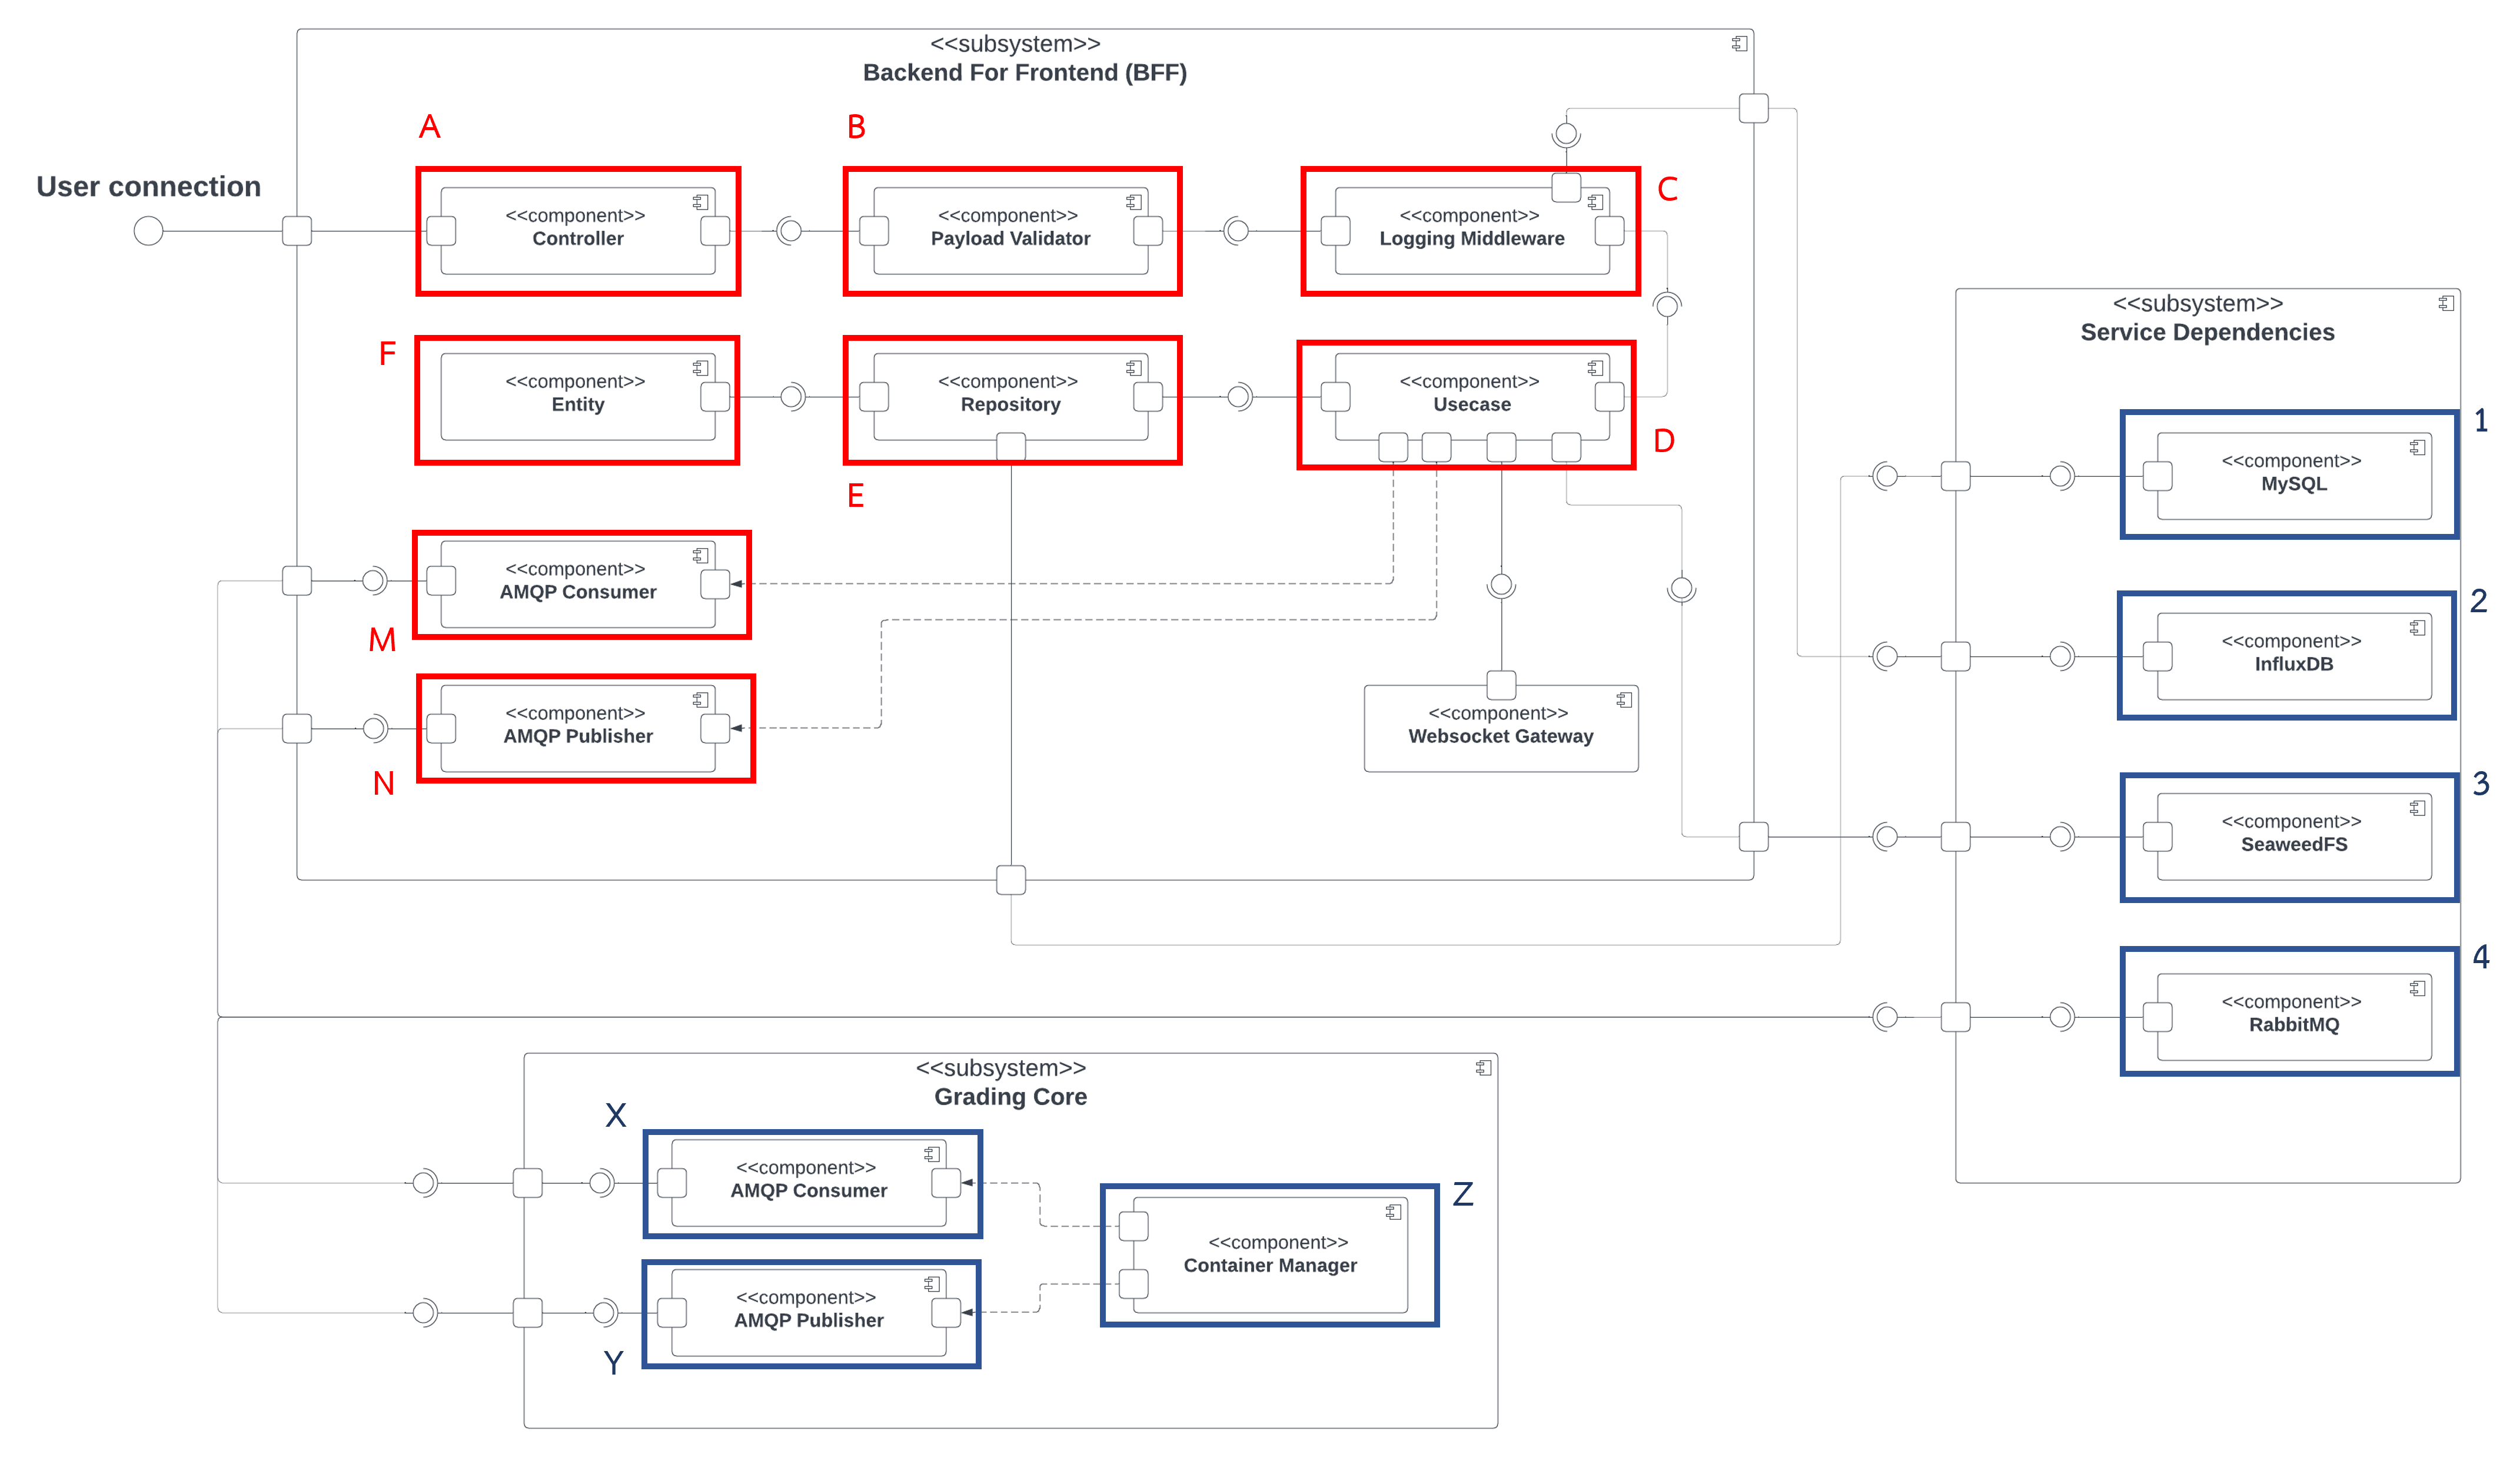
\includegraphics[width=16cm]{figure/diagram/component_v2.png}
    }
    \caption[ภาพแผนผังเเสดงโครงสร้างเเละส่วนประกอบของซอฟต์เเวร์]{แผนภาพเเสดงโครงสร้างเเละส่วนประกอบของซอฟต์เเวร์ วาดด้วย \href{https://lucid.app/}{LucidChart}}
    \label{fig:comp-diagram}
  \end{figure}
}
\begin{enumerate}
  \item \textbf{Backend For Frontend} (BFF) คือระบบย่อยหลักทำหน้าที่การประมวลผลการแสดงออกหน้าเว็บไซต์ โดยมีองค์ประกอบดังนี้
        \begin{itemize}
          \item ส่วนแรกที่ผู้ใช้เชื่อมต่อเข้ามายังระบบ คือ \textbf{Controller} (กรอบแดง A) เป็นส่วนที่คอยรับการเชื่อมต่อของผู้ใช้เข้ามาภายในระบบ
          \item Controller จะส่งต่อการทำงานให่อีกองค์ประกอบหนึ่งที่ชื่อ \textbf{Payload Validator} (กรอบแดง B) ซึ่งจะทำการตรวจสอบความถูกต้องของการเชื่อมต่อ (Connection)
          \item การเชื่อมต่อทั้งหมดจะถูกเก็บเป็นสถิติ ผ่านองค์ประกอบที่ชื่อว่า \textbf{Logging Middleware} (กรอบแดง C)
          \item ส่วนประกอบที่ชื่อ \textbf{Usecase} (กรอบแดง D) จะทำหน้าที่ประมวลผลการเรียกขอข้อมูล (Request) จากผู้ใช้
          \item ถ้าหากต้องการจะเข้าถึงฐานข้อมูล ส่วนประกอบที่ชื่อ \textbf{Repository} (กรอบแดง E) จะทำเข้าถึงฐานข้อมูล และหยิบดึง (Query) ข้อมูลส่งกลับให้ผู้ใช้
          \item ข้อมูลที่ถูกดึงจากฐานข้อมูล มีรูปแบบหรือลักษณะ (Format) ที่ถูกนิยามโดยส่วนประกอบที่ชื่อ \textbf{Entity} (กรอบแดง F)
        \end{itemize}
  \item \textbf{Service Dependencies} คือระบบย่อยสำหรับเก็บข้อมูลโดยเฉพาะ ประกอบด้วยองค์ประกอบที่ทำหน้าที่เก็บข้อมูลรูปแบบใดรูปแบบหนึ่ง ประกอบด้วยองค์ประกอบย่อยดังนี้
        \begin{itemize}
          \item \textbf{MySQL} (กรอบน้ำเงิน 1) เป็นฐานข้อมูลตารางหรือ Relational Database ที่ทำหน้าที่เก็บข้อมูลทั่วไปที่จำเป็นต่อ feature ต่าง ๆ ของซอฟต์แวร์ ตั้งแต่ข้อมูลผู้ใช้ไปจนถึงข้อมูลโจทย์ปัญหา การบ้านหรือข้อสอบทั้งหมด พร้อมทั้งกรณีทดสอบหรือเทสเคส ระบบ BFF เข้าถึงฐานข้อมูลนี้ผ่านองค์ประกอบย่อยชื่อ Repository (กรอบแดง E)
          \item ตามที่ได้กล่าวไปข้่างต้น ข้อมูลการเชื่อมต่อทั้งหมดจะถูกเก็บเป็นสถิติในองค์ประกอบย่อย Logging Middleware โดยข้อมูลการเชื่อมต่อทั้งหมดนั้นจะถูกนำไปเก็บใน \textbf{InfluxDB} (กรอบน้ำเงิน 2) ซึ่งเป็นฐานข้อมูลประเภทห้วงเวลาหรือ Time-series Database ที่จะเก็บข้อมูลการเชื่อมต่อทั้งหมดนั้นในเป็นช่วงๆ เวลาไป
          \item ข้อมูลที่เป็นไฟล์ทั้งหมด ไม่ว่าจะเป็นไฟล์ pdf ของโจทย์ (Assignment), ไฟล์ expected input และ output (Test Case) หรือแม้กระทั่งรูปโปรไฟล์ของผู้ใช้ เป็นต้น จะถูกเก็บในระบบบริการไฟล์หรือ File Service หรือ Filer ชื่อ \textbf{SeaweedFS} (กรอบน้ำเงิน 3)
          \item เนื่องจากระบบซอฟต์แวร์นี้ใช้การ Publish และ Consume ในการแลกเปลี่ยน request และ response ระหว่างระบบย่อย BFF และ Grading Core จึงจำเป็นต้องมี Message Broker ที่จะเก็บพวก message ต่าง ๆ เหล่านี้ ชื่อ \textbf{RabbitMQ} (กรอบน้ำเงิน 4)
        \end{itemize}
  \item \textbf{Grading Core} คือระบบย่อยสำหรับการประมวลผลและ Compile ไฟล์งานหรือโปรแกรมของผู้ใช้ ที่ส่งเข้ามาในระบบให้ตรวจ
        \begin{itemize}
          \item  การรับการเรียกขอ (request) ตรวจงานจากระบบย่อย Backend For Frontend จะทำผ่านองค์ประกอบ \textbf{AMQP Consumer} (กรอบน้ำเงิน X) โดย Consumer นี้จะไปรับคำขอที่ทาง BFF ส่งเข้า RabbitMQ (กรอบน้ำเงิน 4) ผ่าน Publisher ของตัว BFF (กรอบแดง N)
          \item หลังจากตรวจเสร็จ ก็จะส่งผลลัพธ์ผ่านองค์ประกอบ AMQP Publisher ของ
                Grading Core (กรอบนำ้เงิน Y) เข้า RabbitMQ (กรอบน้ำเงิน 4) เพื่อให้องค์ประกอบ AMQP Consumer ที่อยู่ในระบบย่อย BFF (กรอบนำ้เงิน M) Consume ไปเเสดงผลที่หน้าเว็บ
        \end{itemize}
\end{enumerate}
\pagebreak
\subsection{เเผนภาพลำดับการทำงาน}
\thaijustify{
  แผนภาพลำดับการทำงานในรูปที่ \hyperlink{comp-diagram}{3.25} อธิบายกระบวนการทำงานของระบบการตรวจไฟล์งานเขียนโปรแกรมที่ผู้ใช้ส่งเข้ามาให้ตรวจ โดยมีการ actor ดังนี้ (เรียงลำดับขั้นตอน จากบนสุดสู่ล่างสุดของแผนผัง)
}
%%%%%%%%%%% SEQUENCE DIAGRAM %%%%%%%%%%%
\hypertarget{seq-diagram1}{
  \begin{figure}[!h]
    \centering
    \fbox{
      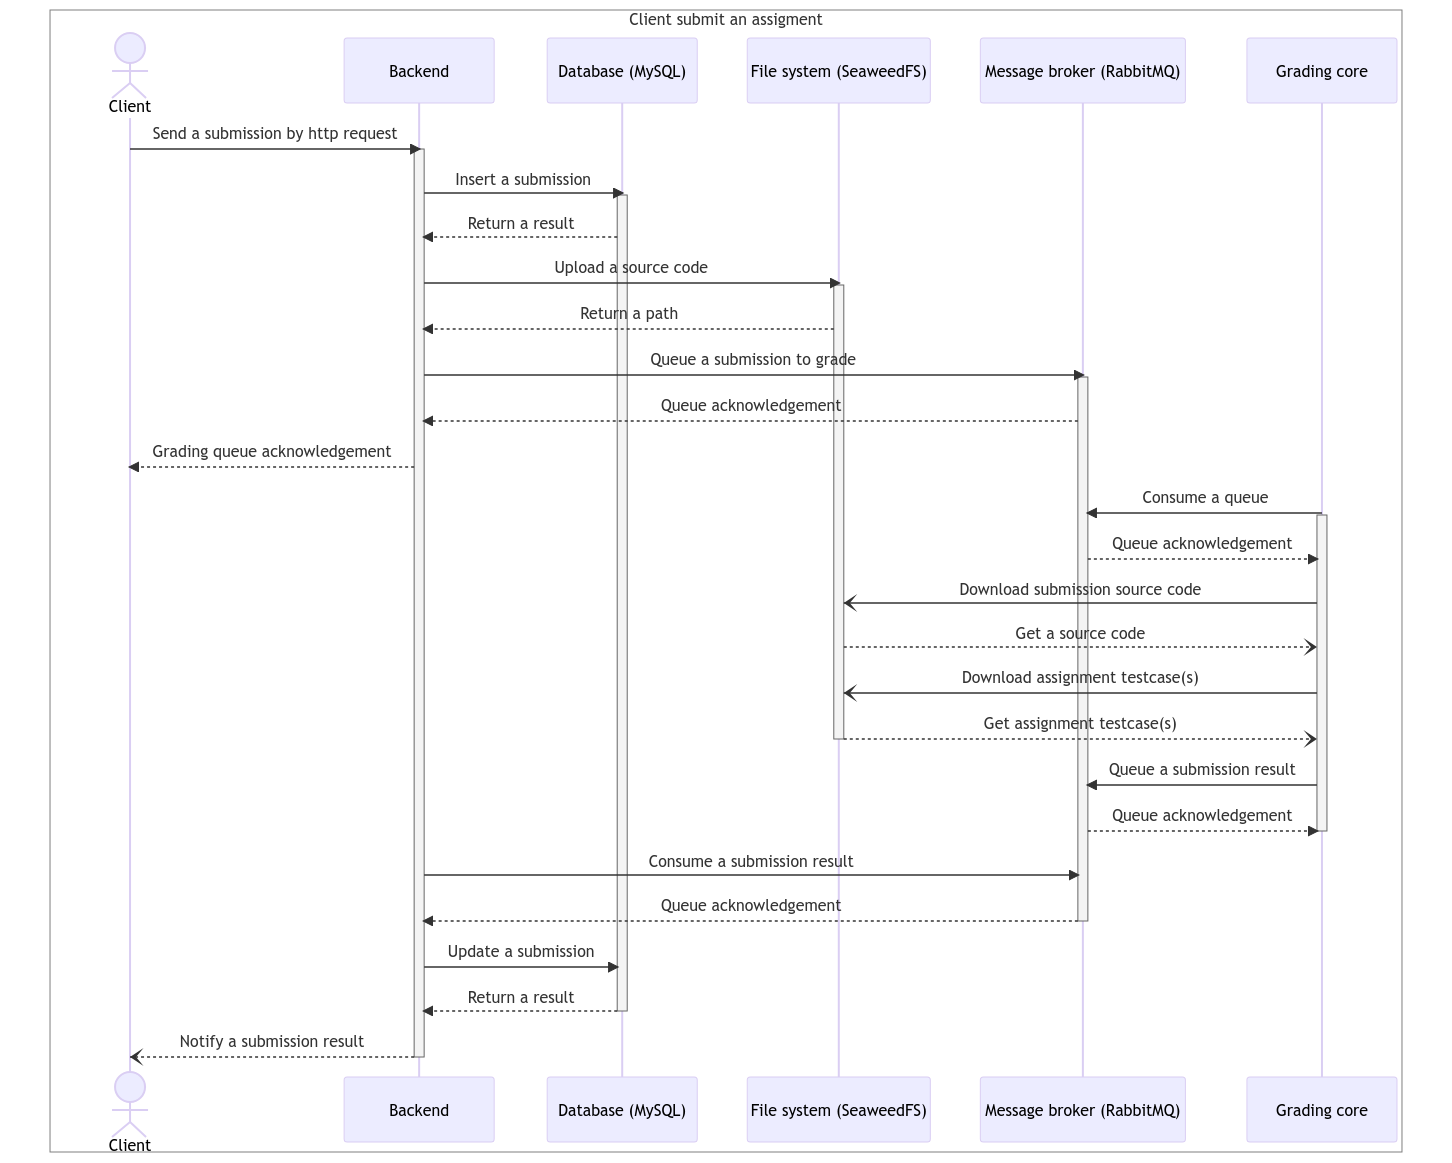
\includegraphics[width=15cm]{figure/diagram/seq-submit_grading-v1.png}
    }
    \caption[ภาพเเผนภาพลำดับการทำงาน]{เเผนภาพลำดับการทำงานของการส่งโปรเเกรมขึ่้นระบบตรวจ วาดด้วย \href{https://mermaid.js.org/}{Mermaid JS}}
    \label{fig:seq-diagram1}
  \end{figure}
}
\begin{itemize}
  \item Client (ผู้ใช้) เริ่มต้นกระบวนการโดยส่งคำขอทาง HTTP ไปยัง Backend เพื่อส่งไฟล์งานเขียนโปรแกรม
  \item Backend (ส่วนหลักของระบบ) รับคำขอและทำการบันทึกไฟล์งานเขียนโปรแกรมลงในฐานข้อมูล MySQL หลังจากนั้นส่งผลการทำงานกลับไปยัง Client พร้อมกับข้อมูลผลการบันทึก
  \item File system (SeaweedFS) ใช้เพื่อเก็บโค้ดของงานและข้อมูลเกี่ยวกับงานต่างๆ เมื่อ Backend อัพโหลดไฟล์งานเขียนให้ File system ก็จะคืน path ที่เก็บไฟล์กลับไปให้ Backend
  \item Message broker (RabbitMQ) มีหน้าที่จัดการการส่งคิวของงานตรวจคะแนนโค้ด หลังจากนั้นส่งการยืนยันการจัดคิวกลับไปยัง Backend แล้วจากนั้น Backend ก็จะส่งการยืนยันต่อไปให้ Client ด้วย
  \item Grading core เป็นส่วนของระบบที่รับผิดชอบในการดำเนินการตรวจคะแนนโค้ด โดยมีกระบวนการดังต่อไปนี้
        \begin{itemize}
          \item Grading core ทำการเช็ค (consume) queue ใน Message broker เพื่อดูว่ามีไฟล์งานเขียนโปรแกรมถูกส่งมาให้ตรวจหรือไม่
          \item Grading core เริ่มต้นกระบวนการโดยการทำการดึงโค้ดของงานและข้อมูลของงานจาก File system
          \item หลังจากที่ทำการตรวจคะแนนเสร็จสิ้น Grading core จะทำการส่งผลการตรวจคะแนนกลับไปยัง Message broker เพื่อจัดคิวการแจ้งผลตรวจคะแนนของงาน
        \end{itemize}
  \item Backend ต่อมาทำการดึงผลการตรวจคะแนนที่ Message broker แจ้งกลับมา และทำการอัพเดทข้อมูลของงานในฐานข้อมูล MySQL พร้อมส่งผลการตรวจคะแนนกลับมา มาแจ้งให้ Client
\end{itemize}
\thaijustify{
  กระบวนการนี้ช่วยในการจัดการและควบคุมกระบวนการตรวจคะแนนงานเขียนโค้ดของระบบ ให้เป็นระเบียบและมีประสิทธิภาพ มีการใช้ Message broker เพื่อรวมและควบคุมการทำงานของ Grading Core และ Backend ให้ทำงานร่วมกันได้อย่างมีประสิทธิภาพ
}

\subsection{แผนผังแสดงโครงสร้างและการนำทางระหว่างหน้าของเว็บไซต์}
\thaijustify{
  จากรูปที่~\ref{fig:nav-map} ข้างต้น เป็นแผนผังโครงสร้างของหน้าเว็บของซอฟต์แวร์ของเรา และการนำทาง ไปมาระหว่างแต่ละหน้าเว็บของซอฟต์แวร์
}
%%%%%%%%%%% NAVIGATION MAP %%%%%%%%%%%
\begin{figure}[H]
  \centering
  \fbox{
    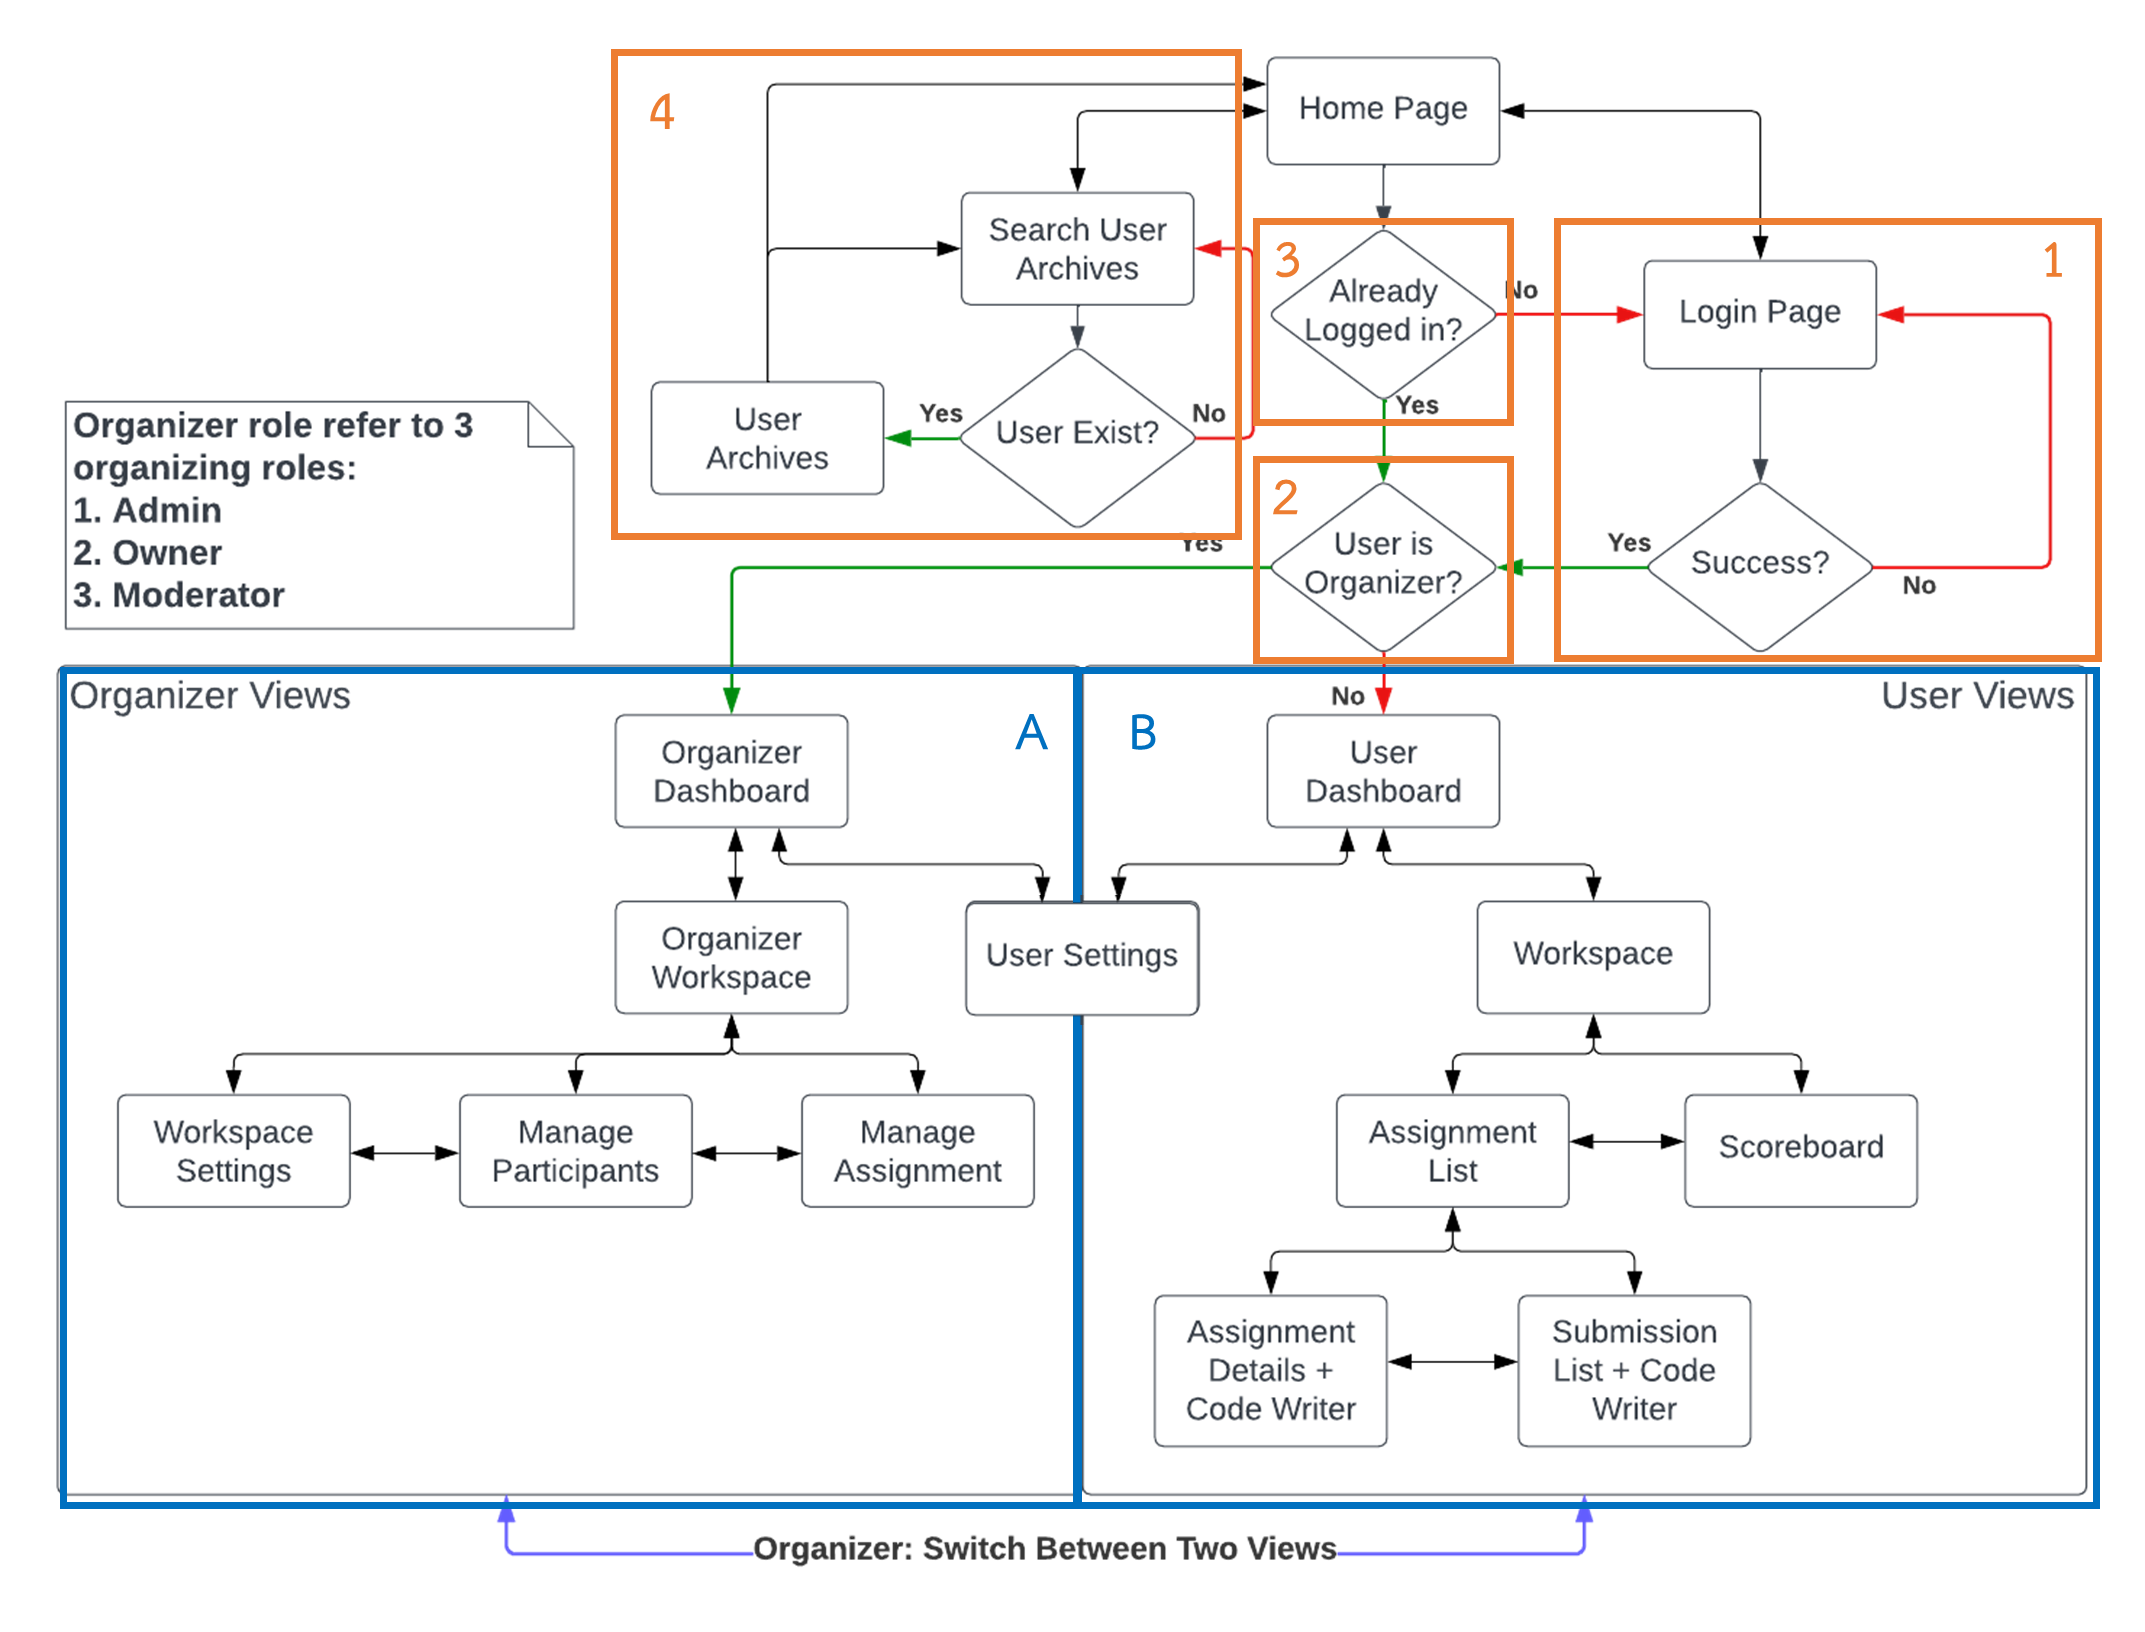
\includegraphics[width=15cm]{figure/diagram/navigation-v2.png}
  }
  \caption[ภาพแผนผังการสัญจรและนำทางระหว่างหน้าของเว็บไซต์]{แผนผังแสดงโครงสร้างและการนำทางระหว่างหน้าของเว็บไซต์ วาดด้วย \href{https://lucid.app/}{LucidChart}}
  \label{fig:nav-map}
\end{figure}
\thaijustify{
  เริ่มต้นจากหน้าแรก (Home page) ของซอฟต์แวร์เรา จากหน้าแรกก็จะสามารถเข้าถึงได้สองหน้า โดยไม่ต้องเข้าสู่ระบบคือหน้าค้นทะเบียนประวัติผู้ใช้เก่า (Search User Archives) (กรอบที่ 4 ในรูปที่~\ref{fig:nav-map}) ซึ่งเป็นจะเป็นหน้าสำหรับกรอกรหัสหรือชื่อของผู้ใช้ที่ต้องการจะค้นทะเบียนประวัติ ถ้าหากค้นแล้วไม่พบผู้ใช้คนดังกล่าว ก็จะถูกตีกลีบไปที่หน้าเดิม แต่ถ้าค้นเจอก็จะถูกนำพามาหน้าแสดงข้อมูลของผู้ใช้ที่ได้ค้นไปเมื่อครู่ (ตรงกับหน้าจอในรูปที่~\ref{fig:ui-archive1})
}
\thaijustify{
  จากหน้าแรก ถ้ากดปุ่ม “Login” ก็จะนำพาผู้ใช้เข้าสู่ระบบยืนยันตัวตน ถ้าหากผู้ใช้ยังไม่ได้เข้าสู่ระบบหรือไม่ได้มี session อยู่ในระบบ ณ ตอนนั้น ก็จะถูกนำพาไปหน้าเข้าสู่ระบบ (Login Page) (กรอบที่ 1 ในรูปที่~\ref{fig:nav-map}) ถ้าหากกรอกข้อมูลผิดอาทิเช่น ชื่อผู้ใช้/อีเมล รหัสผ่าน เป็นต้น ก็จะถูกนำทางกลับไปเข้าสู่หน้าเข้าสู่ระบบหน้าเดิม จนกว่าจะกรอกข้อมูลถูกต้อง
}
\thaijustify{
  ในทางกลับกันถ้าหากผู้ใช้เข้าสู่ระบบแล้ว หรือมี session อยู่ในระบบ ณ ตอนนั้น ก็จะถูกนำพาเข้าสู่แผงควบคุมทันที (กรอบที่ 3 ในรูปที่~\ref{fig:nav-map}) ทั้งนี้ก็ขึ้นอยู่กับบทบาท (role) ของผู้ใช้ว่าเป็น Organizer (หรือบทบาทผู้ดูแลทั้งสามตำแหน่ง: Admin, Owner, และ Moderator ตาม requirements) หรือเป็นผู้ใช้ทั่วไป (หรือ Registered User, Student, Attendee ตาม requirements) บทบาทผู้ใช้แต่ละบทบาท จะถูกนำพาไปสู่รูปแบบแผงควบคุมคนละแบบ (กรอบที่ 2)
}
\thaijustify{
  ถ้าหากเป็น Organizer ก็จะนำพาไปแผงควบคุมที่ในมุมมองของ Organizer (Organizer view) (กรอบ A ในรูปที่ในรูปที่~\ref{fig:nav-map}) ซึ่งสอดคล้องกับ ส่วนประสานผู้ใช้รูปที่~\ref{fig:nav-map} โดยจากแผงควบคุมของ Organizer ก็จะสามารถจะเข้าถึง หน้าตั้งค่าของบัญชีตนเอง (User Settings) และห้องเรียนหรือกลุ่มเรียน (Organizer workspace) ทั้งหมดที่ Organizer คนนั้น ๆ เป็นเจ้าของหรือเข้าถึงได้ หลังจากกดเลือกห้องเรียนหรือกลุ่มเรียนเข้ามาแล้ว ก็จะถูกนำพาเข้ามาหน้าหลักของห้องเรียนหรือกลุ่มเรียนนั้น ๆ (ตรงกับหน้าจอในรูปที่~\ref{fig:nav-map}) ซึ่งสามารถเข้าถึงหน้าตั้งค่าห้องเรียนหรือกลุ่มเรียน (Workspace Settings), หน้าบริหารจัดการสมาชิกห้องเรียนหรือกลุ่มเรียน (Manage Participants), และหน้าบริหารจัดการโจทย์ปัญหาและการบ้าน (Manage Assignment)
}
\thaijustify{
  ถ้าผู้ใช้ไม่ได้มีบทบาทเป็น Organizer แต่เป็นผู้ใช้ทั่วไป (User) ก็จะนำพามาแผงควบคุมในมุมมองของ User (User View) (กรอบ B ในรูปที่ในรูปที่~\ref{fig:nav-map}) ซึ่งตรงกับรูปหน้าจอในรูปที่ในรูปที่~\ref{fig:nav-map} จากหน้าแผงควบคุมดังกล่าว User สามารถจะเข้าถึง หน้าตั้งค่าของบัญชีตนเอง (User Settings) และห้องเรียนหรือกลุ่มเรียน (Workspace) ทั้งหมดที่ User คนนั้น ๆ ได้เข้าร่วมหรือถูกยัดเข้า หลังจากกดเลือกห้องเรียนหรือดักลุ่มเรียนเข้ามาแล้ว ก็จะถูกนำทางมาหน้าหลักของห้องเรียนหรือกลุ่มเรียนนั้น ๆ ซึ่งก็คือหน้าจอแสดงรายการโจทย์ปัญหา (Assignment List) ทั้งหมดในกลุ่มเรียนหรือห้องเรียนนั้น ๆ (เป็นหน้าจอของรูปที่ในรูปที่~\ref{fig:nav-map}) นอกจากหน้ารายการโจทย์ปัญหาแล้ว User ก็สามารถกดไปดูตารางคะแนน (Scoreboard) ของห้องเรียนหรือกลุ่มเรียนนั้นได้ด้วย
}
\thaijustify{
  ถ้าผู้ใช้ทั่วไปหรือ User กดเลือกโจทย์ปัญหาในหน้ารายการแสดงโจทย์ปัญหาและการบ้าน ก็จะถูกนำพาไปหน้าเขียนโปรแกรมซึ่งประกอบแผงเขียนโปรแกรม (Code Writer) กับส่วนแสดงเนื้อหาโจทย์ (Assignment Details) หน้าจอดังกล่าวตรงกับหน้าจอในรูปที่~\ref{fig:nav-map} ผู้ใช้สามารถที่จะเปลี่ยนแผงแสดงเนื้อหาโจทย์เป็นแผงแสดงรายการการส่งโปรแกรมตรวจ (Submission List ได้) ซึ่งตรงกับหน้าจอในรูปที่~\ref{fig:nav-map}
}
\thaijustify{
  ข้อที่ควรรู้เพิ่มเติมคือ ถ้าหากผู้ใช้มีบทบาทเป็น Organizer ผู้ใช้จะสามารถสับเปลี่ยนมุมมอง (Switch View) จาก Organizer เป็น User หรือ User เป็น Organizer ได้ ด้วยปุ่ม “Switch to Normal Mode” หรือ “Switch to Organizer Mode” ตามลำดับ (มีให้เห็นในรูปที่~\ref{fig:ui-org-dashboard1} และ~\ref{fig:ui-assign1} ตรงมุมขวาบน)
}
\pagebreak
\pagebreak
%%%%%%%%%%%%%%%%%% Results and Discussion %%%%%%%%%%%%%%%%%%%%%%
\chapter{ผลการดำเนินงาน}
\thaijustify{
  ในบทที่ 4 จะกล่าวบรรยายและอภิปรายผลลัพธ์กับผลพลอยได้จากการดำเนินการทำโครงการพัฒนาซอฟต์แวร์ Coding Platform ของคณะผู้จัดทำ ซึ่งคณะผู้จัดทำได้นำเอาซอฟต์แวร์ที่พัฒนามาระดับหนึ่ง ที่อยู่ในขั้นพร้อมใช้งานได้ระดับหนึ่งขึ้นไปติดตั้งบนระบบเซิร์ฟเวอร์ แล้วเปิดให้บริการแก่นักศึกษาภาควิชาวิศวกรรมคอมพิวเตอร์ คณะวิศวกรรมศาสตร์ มหาวิทยาลัยเทคโนโลยีพระจอมเกล้าธนบุรี ให้เข้ามาใช้งาน
}
\thaijustify{
  ระหว่างที่เปิดซอฟต์แวร์ของโครงการให้นักศึกษาได้ใช้งาน ทางกลุ่มคณะผู้จัดทำ ได้เก็บข้อมูล (Metrics) และผลลัพธ์ (Result) ไว้มากมาย ซึ่งข้อมูลที่เก็บรวบรวมได้นั้น ล้วนแต่เป็นประโยชน์และให้ความเข้าใจอันลึกซึ้งว่าซอฟต์แวร์ระบบนี้มีสภาพอย่างไร มีจุดแข็งจุด จุดเด่นหรือข้อได้เปรียบตรงไหน มีจุดอ่อนหรือข้อด้อยของระบบอะไรที่ควรปรับปรุง เป็นต้น
}
\section{ผลจากการดำเนินการ}
\thaijustify{
  ในส่วนนี้ ทางคณะผู้จัดทำจะจัดแสดงผลลัพธ์และผลผลิตทั้งหมดที่สะสมมาจาก งานของเราในขั้นตอนการพัฒนาซอฟต์แวร์ที่ผ่านมา กลุ่มเราจะแสดงให้เห็นว่าเครื่องมือและซอฟต์แวร์เชิงระบบแต่ละประเภท แต่ละอย่างที่ได้ทำการศึกษาไปตั้งแต่แรก นั้นนำมาถูกใช้อย่างไร มีบทบาท หน้าที่การงานอย่างไรภายในระบบซอฟต์แวร์ของกลุ่มเรา
}
\thaijustify{
  คณะผู้จัดทำจะแบ่งการอธิบายผลการดำเนินการนี้ ออกเป็นสองส่วน ในด้านหนึ่งคือโครงสร้างพื้นฐานของโครงการซอฟต์แวร์ (Infrastructure) หรือเครื่องมือ (Tools) ของเรา ซึ่งก็คือการนำซอฟต์แวร์เชิงระบบ (Utilities software) อย่างเช่น ฐานข้อมูล MySQL, ระบบจัดการ Container อย่าง Docker หรือระบบจัดการคำขอภายใน (Message broker) ชื่อ RabbitMQ เป็นต้น และอีกด้านหนึ่งก็คือตัวซอฟต์แวร์ส่วนที่กลุ่มคณะผู้จัดทำเขียนขึ้นมาเอง กล่าวคือส่วนนี้เป็นซอร์สโค้ดหลักของโครงงานของกลุ่มเรา
}
\subsection{ระบบซอฟต์แวร์}
ในส่วนนี้ คณะผู้จัดทำจะอธิบายและบรรยายผลการดำเนินการ ด้วยการกล่าวถึงสภาพของซอฟต์แวร์ และหน้าตาของส่วนประสานงานผู้ใช้หลังจากที่ผ่านขั้นพัฒนามาแล้ว โดยจะทำการแบ่งบรรยายเป็นระบบ ๆ ไป
\subsubsection{ระบบบัญชีและข้อมูลสมาชิก}
\begin{figure}[H]
  \centering
  % Already included fbox
  \includegraphics[width=15cm]{figure/new-ui/ui-login1.png}
  \caption[ส่วนประสานต่อผู้ใช้ หน้าเข้าสู่ระบบใหม่]{ส่วนประสานต่อผู้ใช้ หน้าเข้าสู่ระบบอันใหม่}\label{fig:new-ui-login}
\end{figure}
\thaijustify{
  ในรูปที่~\ref{fig:new-ui-login} เป็นหน้าสำหรับล็อกอินเข้าระบบใช้งานทั้งหมดของซอฟต์แวร์ โดยสามารถเลือกล็อกอินได้สองวิธี; ด้วยอีเมลเเละรหัสผ่าน (กรอบสีน้ำเงิน A) และล็อกอินผ่านกูเกิ้ล (กรอบสีแดง B)
}
\begin{figure}[H]
  \centering
  \fbox{
    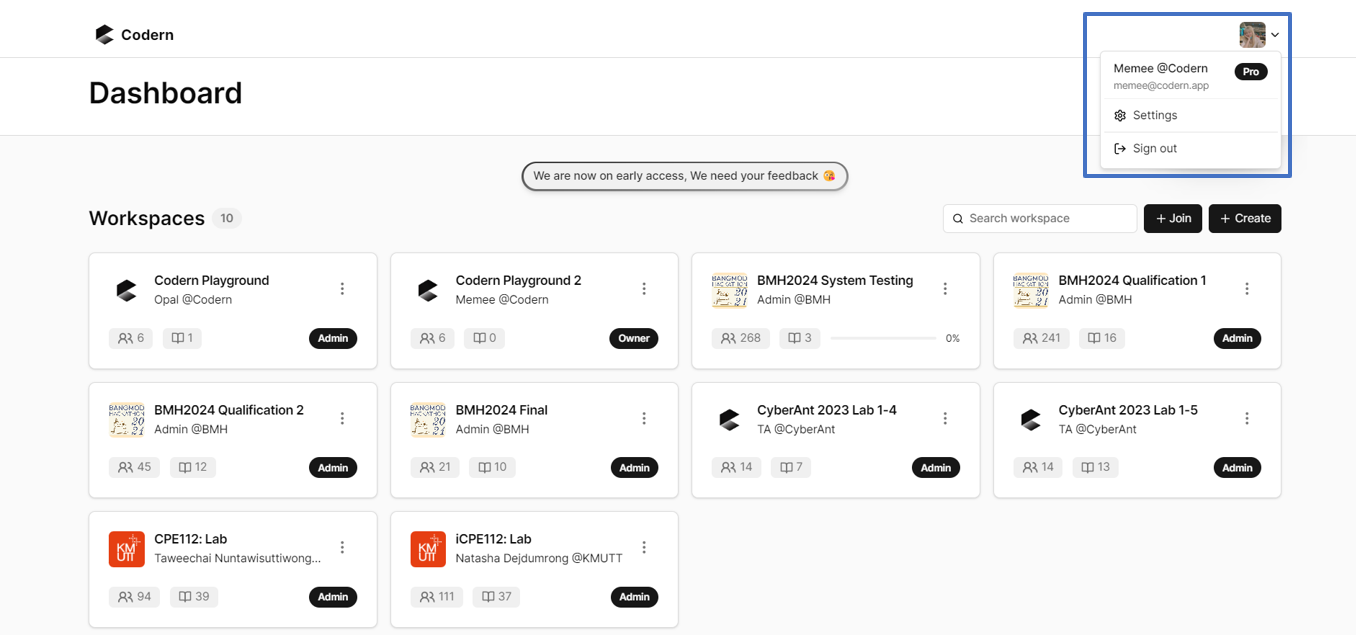
\includegraphics[width=15cm]{figure/new-ui/ui-dashboard5.png}
  }
  \caption[ส่วนประสานต่อผู้ใช้ หน้าเเผงควบคุมใหม่ (กดรูป Avatar)]{ส่วนประสานต่อผู้ใช้ หน้าเเผงควบคุมอันใหม่ หากกดรูป Avatar ตรงมุมขวาบน}
  \label{fig:new-ui-dashboard5}
\end{figure}
\thaijustify{
  เมื่อล็อกอินเข้ามาแล้ว จะพบกับหน้าดังภาพ~\ref{fig:new-ui-dashboard5} หากกดปุ่มไอคอนอวาตาร์รูปของตนบริเวณมุมขวาบนสุดในกรอบสีน้ำเงิน A ในรูปที่~\ref{fig:new-ui-dashboard1} ก็จะปรากฏ Dropdown ลงมาบริเวณกรอบสีน้ำเงิน ประกอบด้วย 2 เมนู ได้แก่ "Settings" และ "Sign out"
}
\begin{figure}[H]
  \centering
  \fbox{
    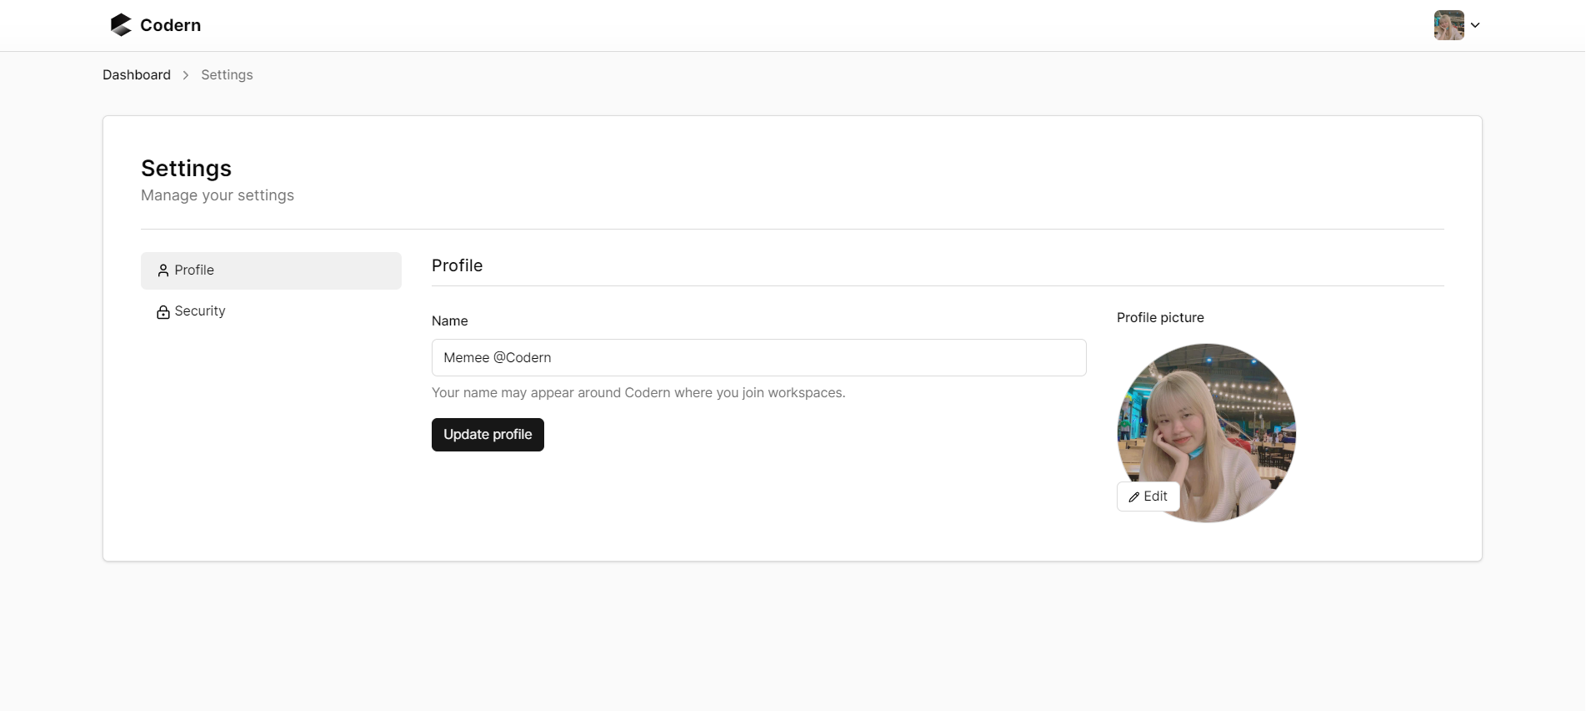
\includegraphics[width=15cm]{figure/new-ui/ui-setting1.png}
  }
  \caption[ส่วนประสานต่อผู้ใช้ หน้าตั้งค่าของผู้ใช้อันใหม่ (กดปุ่ม "Settings")]{ส่วนประสานต่อผู้ใช้ หน้าตั้งค่าของผู้ใช้อันใหม่ หากกดปุ่ม "Settings"}
  \label{fig:new-ui-setting1}
\end{figure}
\thaijustify{
  เมื่อกดเข้ามาภายใน Settings แล้ว จะแบ่งออกเป็น 2 ส่วนย่อย ได้แก่ ส่วนแรกคือ Profile setting ที่ผู้ใช้สามารถแก้ไขชื่อบัญชีผู้ใช้ซึ่งจะแสดงขณะใช้งานภายในเว็บไซต์ และแก้ไขรูปภาพอวาตาร์ของตนได้
}
\begin{figure}[H]
  \centering
  \fbox{
    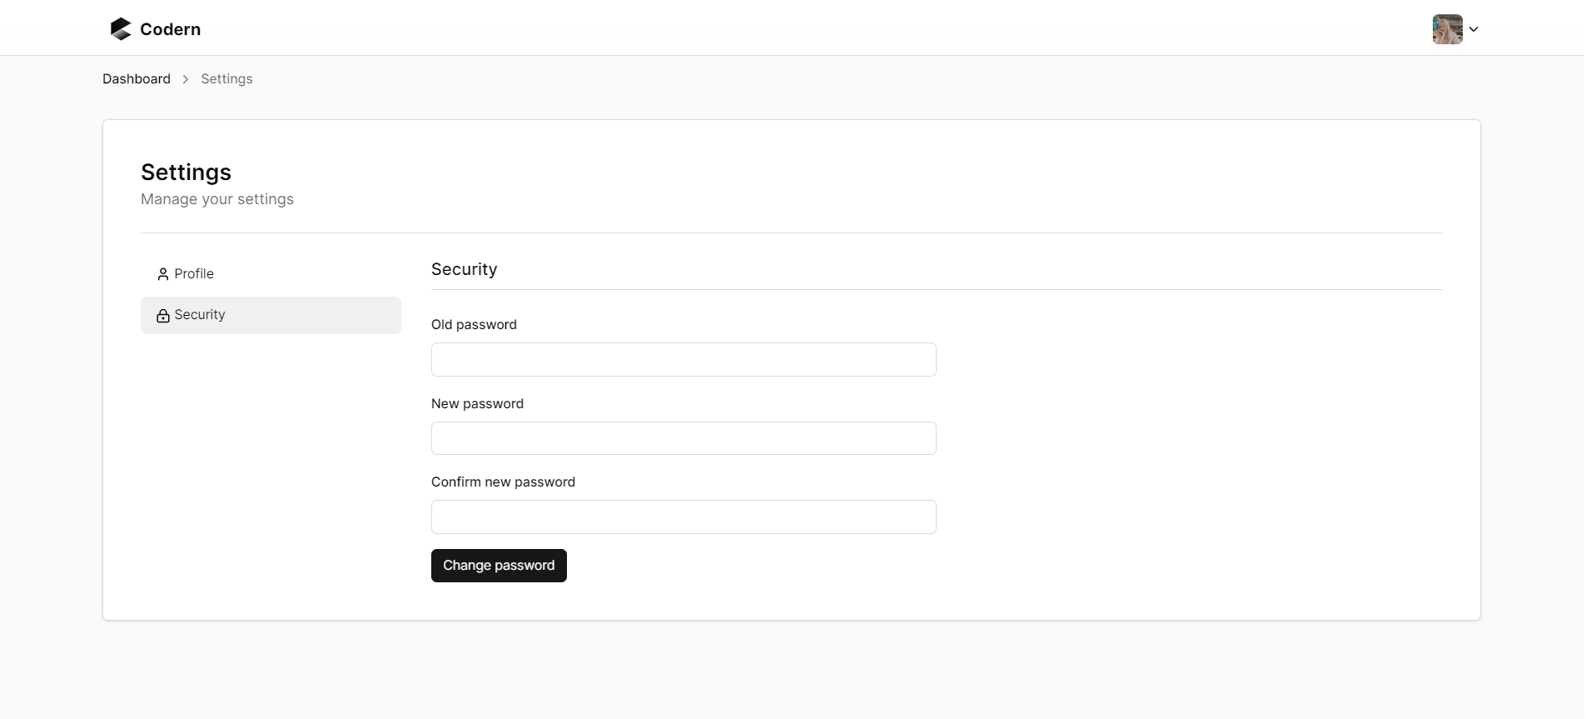
\includegraphics[width=15cm]{figure/new-ui/ui-setting2.png}
  }
  \caption[ส่วนประสานต่อผู้ใช้ หน้าตั้งค่าของผู้ใช้ (กดปุ่ม "Security")]{ส่วนประสานต่อผู้ใช้ หน้าตั้งค่าของผู้ใช้ หากกดปุ่ม "Security"}
  \label{fig:new-ui-setting2}
\end{figure}
\thaijustify{
  และส่วนที่สอง Security setting ที่ผู้ใช้จะสามารถเปลี่ยนรหัสผ่านเข้าบัญชี ดังรูปที่~\ref{fig:new-ui-setting2} โดยจะเปลี่ยนรหัสผ่านบัญชีได้โดยการกรอกรหัสผ่านเก่าให้ถูกต้อง จากนั้นก็กรอกรหัสผ่านใหม่ที่ต้องการ และทำการยืนยันรหัสผ่านใหม่ซ้ำอีกครั้ง เมื่อกรอกรหัสทั้งหมดถูกต้อง เพียงกดปุ่ม "Change password" ก็จะสามารถเปลี่ยนรหัสผ่านบัญชีใหม่ได้ แต่ถ้ากดปุ่ม Sign out ในรูปที่~\ref{fig:new-ui-dashboard5} จะกลับไปสู่หน้าล็อกอินแรกสุดของระบบ ดังรูปที่~\ref{fig:new-ui-login}
}

\subsubsection{ระบบห้องเรียนและกลุ่มเรียน}
\begin{figure}[H]
  \centering
  \fbox{
    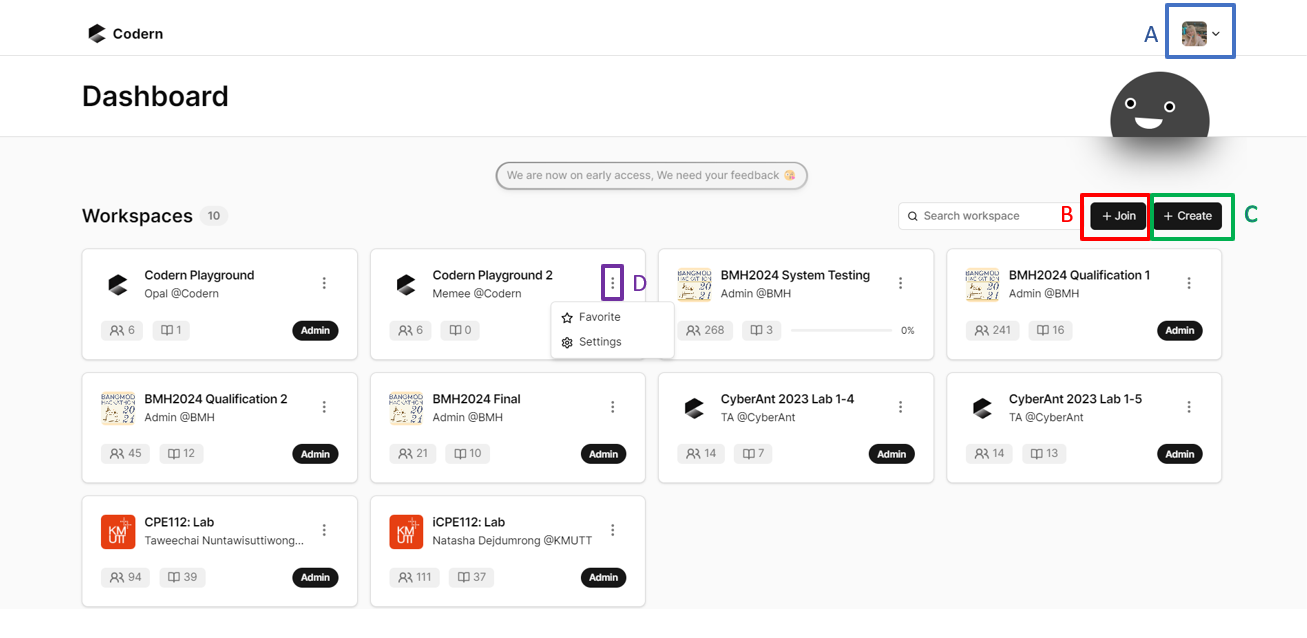
\includegraphics[width=15cm]{figure/new-ui/ui-dashboard1.png}
  }
  \caption[ส่วนประสานต่อผู้ใช้ หน้าเเผงควบคุมอันใหม่]{ส่วนประสานต่อผู้ใช้ หน้าเเผงควบคุมอันใหม่}\label{fig:new-ui-dashboard1}
\end{figure}

\thaijustify{
  เมื่อเข้าสู่ระบบเรียบร้อยแล้ว ระบบจะนำไปสู่หน้าแสดงรายการห้องทั้งหมดที่ผู้ใช้ได้เข้าร่วม ดังรูปที่~\ref{fig:new-ui-dashboard1} ส่วนต่อประสานกับผู้ใช้หน้าแสดงรายการห้องที่ผู้ใช้ได้เข้าร่วมอยู่ในปัจจุบัน ตำแหน่งในกรอบสีแดง B ผู้ใช้สามารถที่จะกดเข้าร่วมห้องใหม่ได้ที่ปุ่ม “Join” และหากบัญชีผู้ใช้มีตำแหน่ง Type pro จะสามารถมองเห็นและใช้งานปุ่ม "Create" ในกรอบสีเขียว C เพื่อสร้างห้องใหม่ได้ ซึ่งบัญชีผู้ใช้ Type pro นี้ต้องให้ผู้พัฒนาซอฟต์แวร์ เป็นผู้ตั้งให้เท่านั้น อีกทั้งในรายการแสดงห้องที่เข้าร่วมด้านล่าง เมื่อกด Kebub menu ไอคอนในกรอบสีม่วง D จะแสดง Dropdown รายการตั้งห้องที่เข้าร่วมนั้นเป็นรายการโปรดได้ และหากผู้ใช้เป็นผู้ดูแลของห้องเรียนนั้นๆ จะสามารถเข้าดูและแก้ไขการตั้งค่าของห้องเรียนนั้นๆ ได้
}
\begin{figure}[H]
  \centering
  \fbox{
    \includegraphics[width=15cm]{figure/new-ui/ui-dashboard2.png}
  }
  \caption[ส่วนประสานต่อผู้ใช้ หน้าเเผงควบคุมอันใหม่ (กดปุ่ม "Join")]{ส่วนประสานต่อผู้ใช้ หน้าเเผงควบคุมอันใหม่ หลังกดปุ่ม "Join"}\label{fig:new-ui-dashboard2}
\end{figure}
\thaijustify{
  โดยเมื่อผู้ใช้กดเข้าร่วมห้องใหม่ที่ปุ่ม “Join” แล้ว จะปรากฏกล่องข้อความแจ้งเตือนเพื่อแสดงข้อความ ดังรูปที่~\ref{fig:new-ui-dashboard2} ซึ่งต้องการให้ผู้ใช้กรอกรหัสเข้าร่วมห้องเรียนที่ได้มีการสร้างไว้ก่อนอยู่แล้วได้
}

\begin{figure}[H]
  \centering
  \fbox{
    \includegraphics[width=15cm]{figure/new-ui/ui-dashboard3.png}
  }
  \caption[ส่วนประสานต่อผู้ใช้ หน้าเเผงควบคุมอันใหม่ (กดปุ่ม "Create")]{ส่วนประสานต่อผู้ใช้ หน้าเเผงควบคุมอันใหม่ หลังกดปุ่ม "Create"}
  \label{fig:new-ui-dashboard3}
\end{figure}
\thaijustify{
  แต่หากผู้ใช้มีประเภทบัญชีผู้ใช้เป็น Pro เมื่อกดปุ่ม “Create” แล้ว จะนำไปสู่หน้าสร้างห้องเรียนใหม่ ดังรูปที่~\ref{fig:new-ui-dashboard3} ซึ่งต้องการให้ผู้ใช้ตั้งชื่อห้องเรียนและ   กำหนดภาพไอคอนของห้องเรียน เมื่อกดปุ่ม Create แล้ว ห้องเรียนใหม่ก็จะถูกสร้างขึ้น
}
\pagebreak
\thaijustify{
  โดยหลังจากกดเข้าสู่ห้องเรียนเรียบร้อยแล้ว หากเป็นผู้ดูแลระบบ จะสามารถมองเห็น Tab "Settings" บริเวณกรอบสีม่วง D รูปที่~\ref{fig:new-ui-assign2} ได้ หน้าในรูปที่~\ref{fig:new-ui-setting-general} จะปรากฎขึ้นมา ซึ่งหน้าข้างต้นเป็นหน้าสำหรับตั้งค่าข้อมูลต่าง ๆ ภายในห้องเรียนหรือกลุ่มเรียนนั้น ๆ ซึ่งมีเฉพาะผู้ดูเเลเท่านั้นที่จะสามารถเข้าไปดูเเละเเก้ไขได้เท่านั้น โดยจะแบ่งเป็น 3 ส่วนย่อย ประกอบไปด้วย General settings ซึ่งจะเป็นเมนูแรกสุดดังรูปที่~\ref{fig:new-ui-setting-general} ตามมาด้วย Admin settings และ Invitation settings ดังรูปที่~\ref{fig:new-ui-setting-admin} และรูปที่~\ref{fig:new-ui-setting-invitation1} ตามลำดับ
}

\begin{figure}[H]
  \centering
  \fbox{
    \includegraphics[width=15cm]{figure/new-ui/ui-setting-general.png}
  }
  \caption[ส่วนประสานต่อผู้ใช้ หน้าตั้งค่า Workspace ของผู้ดูเเลระบบ (ใน "General")]{ส่วนประสานต่อผู้ใช้ หน้าตั้งค่า Workspace ใน Section "General" ในมุมมองของผู้ดูเเลระบบ}
  \label{fig:new-ui-setting-general}
\end{figure}
\thaijustify{
  โดย "General settings" ดังรูปที่~\ref{fig:new-ui-setting-general} จะเป็นหน้าสำหรับการแก้ไขข้อมูลทั่วไปของห้องเรียนนั้น ๆ เช่น ชื่อของห้องเรียน หรือ รูปรูปที่แสดง และที่สำคัญยังสามารถลบห้องเรียนนั้น ๆ ได้เมื่อกดที่ปุ่ม Delete this workspace ภายใน Danger zone ซึ่งการลบห้องเรียนนั้นจะเป็นการลบอย่างถาวร ข้อมูลทั้งหมดจะถูกลบโดยไม่สามารถกู้คืนได้อีก
}

%%%%%%%%%%% ASSIGN SETTINGS - ADMIN %%%%%%%%%%%
\hypertarget{new-ui-setting-admin}{
  \begin{figure}[H]
    \centering
    \includegraphics[width=15cm]{figure/new-ui/ui-setting-admin.png}
    \caption[ส่วนประสานต่อผู้ใช้ หน้าตั้งค่า Workspace ของผู้ดูเเลระบบ (ใน "Admin")]{ส่วนประสานต่อผู้ใช้ หน้าตั้งค่า Workspace ใน Section "Admin" ในมุมมองของผู้ดูเเลระบบ}
    \label{fig:new-ui-setting-admin}
  \end{figure}
}

\thaijustify{
  ในของ "Admin Settings" ดังรูปที่~\ref{fig:new-ui-setting-admin} จะเป็นหน้าสำหรับการเพิ่มแอดมินหรือผู้ดูแลเข้าสู่ห้องเรียนนั้น ๆ โดยจะประกอบด้วยกล่องค้นหา หากค้นหาพบคนที่ต้องการแล้ว เมื่อกดปุ่ม "Add admin" จะเป็นการเพิ่มผู้ดูแลคนนั้น ๆ เข้าสู่ห้องเรียน
}

%%%%%%%%%%% ASSIGN SETTINGS - INVITATION %%%%%%%%%%%
\hypertarget{new-ui-setting-invitation1}{
  \begin{figure}[H]
    \centering
    \fbox{
      \includegraphics[width=15cm]{figure/new-ui/ui-setting-invitation1.png}
    }
    \caption[ส่วนประสานต่อผู้ใช้ หน้าตั้งค่า Workspace ของผู้ดูเเลระบบ (ใน "Invitation")]{ส่วนประสานต่อผู้ใช้ หน้าตั้งค่า Workspace ใน Section "Invitation" ในมุมมองของผู้ดูเเลระบบ}
    \label{fig:new-ui-setting-invitation1}
  \end{figure}
}

\thaijustify{
  สุดท้ายในส่วนของ "Invitation Settings" ดังรูปที่~\ref{fig:new-ui-setting-invitation1} เป็นหน้าสำหรับการเชิญผู้ใช้ทั่วไปเข้าสู่ห้องเรียนนั้น ๆ โดยตัวผู้ดูแล ซึ่งทำได้โดยกดปุ่ม "Create" บริเวณกล่องสีเขียว จะปรากฏกล่องข้อความแจ้งเตือน (รูปที่~\ref{fig:new-ui-setting-invitation2} ในภาคผนวก)เพื่อให้ผู้ดูแลกำหนดวันที่สามารถเริ่มใช้รหัสได้ และวันสิ้นสุดการใช้งานของรหัสนั้นๆ และเมื่อผู้ใช้กรอกรหัสดังกล่าวลงในกล่อง "Invitation code" ในรูปที่~\ref{fig:new-ui-dashboard2} และกดปุ่ม "Join" จะเป็นการเข้าร่วมห้องเรียนนั้น ๆ
}
\subsubsection{ระบบโจทย์ปัญหาและการส่งงาน}
\begin{figure}[H]
  \centering
  \fbox{
    \includegraphics[width=15cm]{figure/new-ui/ui-assign1.png}
  }
  \caption[ส่วนประสานต่อผู้ใช้ หน้ารายการโจทย์ปัญหา]{ส่วนประสานต่อผู้ใช้ หน้ารายการโจทย์ปัญหา}
  \label{fig:new-ui-assign1}
\end{figure}
\begin{figure}[H]
  \centering
  \fbox{
    \includegraphics[width=15cm]{figure/new-ui/ui-code1.png}
  }
  \caption[ส่วนประสานต่อผู้ใช้ หน้าแผงเขียนโปรแกรมกับโจทย์ปัญหา]{ส่วนประสานต่อผู้ใช้ หน้าโจทย์ปัญหาและแผงเขียนโปรแกรม}
  \label{fig:new-ui-code1}
\end{figure}
\thaijustify{
  ถ้าหากกดรายการการบ้าน โจทย์ปัญหา มาสักรายการ (ในรูปที่~\ref{fig:new-ui-assign1}) ก็จะนำพามาสู่หน้าโจทย์ปัญหาในรูปที่~\ref{fig:new-ui-code1} โดยในหน้านี้ในโซนที่ 1 จะเป็นช่องแผงเขียนโปรแกรม สามารถที่จะเขียนโปรแกรมภาษาคอมพิวเตอร์ในโซนนี้ได้ ในโซนที่ 2 จะเป็นแสดงรายละเอียดของโจทย์ตั้งแต่เนื้อหาโจทย์ ไปจนถึงจำนวนหน่วยความจำที่ใช้ได้ (Memory Limit) และระยะเวลาที่ใช้ในการหาคำตอบ (Runtime Limit) ถ้าหากต้องการส่งก็สามารถที่จะกดปุ่ม “Submit” ที่กรอบน้ำเงิน A เพื่อส่งงานเขียนโปรแกรมไปให้ตรวจ และอีกทั้งก่อนส่ง ก็ยังสามารถที่จะตั้งค่าและเลือก compiler ที่ต้องการจะใช้ในการตรวจงานเขียนโปรแกรมดังกล่าวได้ที่ Dropdown ที่กรอบน้ำเงิน B หลังจากผู้ใช้กดส่งไปตรวจแล้ว สามารถติดตามผลได้ในรายการ submission ซึ่งสามารถกดดูได้ตรงกรอบสีเขียว C ในรูปที่~\ref{fig:new-ui-code1}
}
\begin{figure}[H]
  \centering
  \fbox{
    \includegraphics[width=15cm]{figure/new-ui/ui-code2.png}
  }
  \caption[ส่วนประสานต่อผู้ใช้ หน้าแผงเขียนโปรแกรมและรายการส่งพร้อทผลการตรวจ]{ส่วนประสานงานต่อผู้ใช้ หน้าโจทย์ปัญหาและแผงเขียนโปรแกรม พร้อมรายการส่งเเละผลการตรวจทั้งหมด}
  \label{fig:new-ui-code2}
\end{figure}
\thaijustify{
  หลังจากกดเลือก Tab ชื่อ "Submission" เเผงแสดงผลเนื้อหาโจทย์ จะถูกเปลี่ยนมาเป็นรายการผลส่งการตรวจทั้งหมด ดังรูปที่~\ref{fig:new-ui-code2} โดยในรายการก็จะแสดงรายละเอียดการส่งแต่ละครั้งที่ผู้ใช้ส่ง มีรายละเอียดต่าง ๆ อาทิเช่น วันเวลาที่ส่งคำตอบ ภาษาที่ส่งไปตรวจ และผลการตรวจของแต่ละ Test Case (ถ้า Correct แปลว่า output ของโปรแกรมที่เขียนให้ผลตรงตาม Test Case ที่โจทย์ข้อนี้ตั้งไว้, แต่ถ้า Wrong ก็จะแสดงว่า output ของโปรแกรมที่เขียนไม่ได้ให้ผลตรงตาม Test Case ที่โจทย์ข้อนี้ตั้งไว้) และยังมีปุ่ม "View code" สำหรับกดดูคำตอบที่ส่งไปตรวจได้อีกด้วย ดังรูปที่~\ref{fig:new-ui-code3}
}

\begin{figure}[H]
  \centering
  \fbox{
    \includegraphics[width=15cm]{figure/new-ui/ui-code3.png}
  }
  \caption[ส่วนประสานต่อผู้ใช้ หน้าแผงเขียนโปรแกรม (กดแสดงคำตอบที่ได้ทำการส่งตรวจแล้ว)]{ส่วนประสานงานต่อผู้ใช้ หน้าแสดงคำตอบที่ได้ทำการส่งตรวจแล้ว}
  \label{fig:new-ui-code3}
\end{figure}
\begin{figure}[H]
  \centering
  \fbox{
    \includegraphics[width=15cm]{figure/new-ui/ui-assign2.png}
  }
  \caption[ส่วนประสานต่อผู้ใช้ หน้ารายการโจทย์ปัญหาของผู้ดูเเลระบบ]{ส่วนประสานต่อผู้ใช้ หน้ารายการโจทย์ปัญหา ในมุมมองของผู้ดูเเลระบบ}
  \label{fig:new-ui-assign2}
\end{figure}
\thaijustify{
  ในอีกฝั่ง ส่วนของผู้ดูแลในรูปที่~\ref{fig:new-ui-assign2} ก็จะแสดงผลคล้ายคลึงกับฝั่งของผู้ใช้ในรูปที่~\ref{fig:new-ui-assign1} มีความต่างที่มีปุ่ม “Create” (กรอบสีเขียว A) สำหรับสร้างโจทย์ใหม่เพิ่มเข้ามา ซึ่งเป็นฟอร์มสำหรับสร้างการบ้าน โจทย์ปัญหาหรือข้อสอบ สำหรับให้อาจารย์ผู้สอนหรือเจ้าของห้องได้ใช้ เมื่อกดแล้วจะนำไปสู่รูปที่~\ref{fig:new-ui-assign5}
}
%%%%%%%%%%% CREATE ASSIGNMENT %%%%%%%%%%%
\begin{figure}[H]
  \centering
  % Already included fbox
  \includegraphics[width=15cm]{figure/new-ui/ui-assign5.png}
  \caption[ส่วนประสานต่อผู้ใช้ หน้าฟอร์มสร้างโจทย์ปัญหา]{ส่วนประสานต่อผู้ใช้ หน้าฟอร์มสร้างโจทย์ปัญหาของผู้ดูเเลระบบ}
  \label{fig:new-ui-assign5}
\end{figure}
\thaijustify{
  ซึ่งภายในรูปที่~\ref{fig:new-ui-assign5} นั้น อาจารย์หรือผู้ดูแลสามารถเพิ่มโจทย์ปัญหาใหม่เข้าสู่ระบบได้ โดยจะมีข้อมูลของโจทย์ปัญหาให้กรอกตามกำหนด ประกอบไปด้วย ชื่องาน, รายละเอียดงาน, ระดับความยาก, จำนวนหน่วยความจำที่ใช้ได้ (Memory Limit), ระยะเวลาที่ใช้ในการหาคำตอบ (Runtime Limit), รายละเอียดของโจทย์, ตัวอย่างผลลัพธ์ (Test case) และนอกจากนี้ยังสามารถกด Preview เพื่อดูตัวอย่างของโจทย์ที่จะออกมาได้อีกด้วย เมื่อกดปุ่ม "Create" ด้านล่างสุด โจทย์ปัญหาก็จะถูกสร้างขึ้น
}
\thaijustify{
  ต่อมา จากรูป ~\ref{fig:new-ui-assign2} บริเวณกรอบสีน้ำเงิน B จะมีปุ่มรูป "Meatballs Menu" ท้ายสุดของแต่ละแถวเพิ่มขึ้นมา ซึ่งเมื่อกดแล้วจะปรากฏ Dropdown ให้เลือก 3 ส่วน ได้แก่ Try คือการลองทำโจทย์นั้น ๆ, Edit คือการแก้ไขข้อมูลของโจทย์ และ Delete คือการลบโจทย์ข้อนั้น ๆ (รูปที่~\ref{fig:new-ui-assign8},  \ref{fig:new-ui-assign6}, \ref{fig:new-ui-assign7} ตามลำดับในภาคผนวก)
}
\thaijustify{
  ส่วนภายในหน้า Edit Assignment (ดังรูปที่~\ref{fig:new-ui-assign6} ในภาคผนวก) จะเป็นหน้าที่อาจารย์หรือผู้ดูแลสามารถแก้ไขข้อมูลของโจทย์ปัญหานั้นๆ ที่ถูกสร้างไว้แล้วได้ โดยจะสามารถแก้ไขข้อมูลได้ทั้งหมด ตั้งแต่ ชื่องาน, รายละเอียดงาน, ระดับความยาก, จำนวนหน่วยความจำที่ใช้ได้ (Memory Limit), ระยะเวลาที่ใช้ในการหาคำตอบ (Runtime Limit), รายละเอียดของโจทย์ และตัวอย่างผลลัพธ์ (Test case)
}
\thaijustify{
  อีกทั้งจากรูป รูปที่~\ref{fig:new-ui-assign2} หากกดลงไปที่รายการโจทย์แต่ละข้อ (กรอบสีแดง C) จะนำไปสู่หน้าแสดงรายชื่อผู้ที่ส่งคำตอบของโจทย์ข้อนั้นๆ เข้ามา (รูปที่~\ref{fig:new-ui-assign3}) ซึ่งแสดงรายละเอียดชื่อผู้ส่ง วันเวลาที่ส่งคำตอบเข้ามา ภาษาที่ใช้ สถานะ และผลคะแนนที่ได้ของโปรแกรมนั้น ๆ และในคอลัมน์ท้ายสุดของแต่ละรายชื่อ จะสามารถกดปุ่ม "View code" เพื่อแสดงคำตอบของผู้ที่ส่งคำตอบของโจทย์นั้นๆ เข้ามาได้ ดังรูปที่~\ref{fig:new-ui-assign4} ทั้งยังสามารถกด "Copy to clipboard" เพื่อคัดลอกคำตอบทั้งหมดได้ในครั้งเดียวอีกด้วย
}
\begin{figure}[H]
  \centering
  \fbox{
    \includegraphics[width=15cm]{figure/new-ui/ui-assign3.png}
  }
  \caption[ส่วนประสานต่อผู้ใช้ หน้าแสดงรายชื่อผู้ที่ส่งคำตอบของโจทย์ปัญหา]{ส่วนประสานต่อผู้ใช้ หน้าแสดงรายชื่อผู้ที่ส่งคำตอบของโจทย์ปัญหา ในมุมมองของผู้ดูเเลระบบ}
  \label{fig:new-ui-assign3}
\end{figure}
\begin{figure}[H]
  \centering
  \fbox{
    \includegraphics[width=15cm]{figure/new-ui/ui-assign4.png}
  }
  \caption[ส่วนประสานต่อผู้ใช้ หน้าแสดงคำตอบของผู้ที่ส่งคำตอบของโจทย์ปัญหา]{ส่วนประสานต่อผู้ใช้ หน้าแสดงคำตอบของผู้ที่ส่งคำตอบของโจทย์ปัญหา ในมุมมองของผู้ดูเเลระบบ}
  \label{fig:new-ui-assign4}
\end{figure}
\pagebreak
\subsection{ระบบโครงสร้างพื้นฐานและเครื่องมือ}
นอกจากตัวระบบซอฟต์แวร์ที่เป็นชิ้นงานหลักของโครงการนี้แล้ว ทางคณะผู้จัดทำก็จะแสดงสภาพและหน้าตาของเครื่องมือและซอฟต์แวร์โครงสร้างพื้นฐานต่าง ๆ ที่ใช้ประกอบการทำงานของตัวซอฟต์แวร์หลักของโครงการด้วยเช่นกันในส่วนหัวข้อนี้
\subsubsection{ระบบบริหาร Container}
\thaijustify{
  สำหรับระบบบริหารและดูแล Container ที่ใช้ในการรันโปรแกรมต่าง ๆ ของโครงการ กลุ่มของเราใช้ Kubernetes บริหาร Container ควบคู่กับ Docker
}
\begin{figure}[H]
  \centering
  \includegraphics[width=15cm]{figure/results/kubectl.png}
  \caption[รายการ Pods ของ Kubernetes]{รายการแสดง Pods ที่ Kubernetes กำลังรันอยู่บนเซิร์ฟเวอร์ขณะนั้น}
  \label{fig:res-kube}
\end{figure}
\thaijustify{
  กลุ่มของเราใช้ Kubernetes เป็นช่องการในการนำซอฟต์แวร์ที่พร้อมใช้งาน ลงเปิดใช้งานบนเซิร์ฟเวอร์ (หรือเรียกว่าการ Deploy) สาเหตุที่กลุ่มเราใช้ Kubernetes เพราะความสามารถของ Kubernetes ในการใช้ Rollout เพื่อปรับเปลี่ยนเวอร์ชั่นของซอฟต์แวร์ โดยที่ไม่จำเป็นต้องปิดซอฟต์แวร์เปิดใหม่ ด้วยความสามารถนี้ ทางกลุ่มสามารถที่จะพัฒนาแล้วใส่ Feature ใหม่เข้าซอฟต์แวร์ได้อย่างราบรื่น โดยไม่เป็นที่รบกวนผู้ใช้ที่กำลังใช้งานซอฟต์แวร์ดังกล่าวอยู่มากนัก ขณะกำลังทำการเปลี่ยนเวอร์ชั่นซอฟต์แวร์
}
\begin{figure}[H]
  \centering
  \includegraphics[width=15cm]{figure/results/dockerps.png}
  \caption[รายการ Container แสดงด้วย Docker]{รายการแสดง Container ทั้งหมดที่เซิร์ฟเวอร์กำลังรันอยู่ขณะนั้น ดูด้วย Docker}
  \label{fig:res-docker}
\end{figure}
\thaijustify{
  กลุ่มของเราใช้ Kubernetes เป็นช่องการในการนำซอฟต์แวร์ที่พร้อมใช้งาน ลงเปิดใช้งานบนเซิร์ฟเวอร์ (หรือเรียกว่าการ Deploy) สาเหตุที่กลุ่มเราใช้ Kubernetes เพราะความสามารถของ Kubernetes ในการใช้ Rollout เพื่อปรับเปลี่ยนเวอร์ชั่นของซอฟต์แวร์ โดยที่ไม่จำเป็นต้องปิดซอฟต์แวร์เปิดใหม่ ด้วยความสามารถนี้ ทางกลุ่มสามารถที่จะพัฒนาแล้วใส่ Feature ใหม่เข้าซอฟต์แวร์ได้อย่างราบรื่น โดยไม่เป็นที่รบกวนผู้ใช้ที่กำลังใช้งานซอฟต์แวร์ดังกล่าวอยู่มากนัก ขณะกำลังทำการเปลี่ยนเวอร์ชั่นซอฟต์แวร์
}
\thaijustify{
  ส่วน Docker กลุ่มเราใช้ในสำหรับเป็นเครื่องมือที่ใช้ควบคู่กับการพัฒนาซอฟต์แวร์ กล่าวคือกลุ่มเราใช้ Docker สำหรับในการเรียกดู Container มาตรวจสอบทีละตัว นับว่าเป็นประโยชน์อย่างมากกับการสืบหาข้อผิดพลาด หรือตรวจวินิจฉัยหาสาเหตุที่ทำให้ระบบล่ม
}
\subsubsection{ระบบ CI/CD}
\thaijustify{
  สำหรับระบบการทำ Pipeline เพื่อนำซอฟต์แวร์ไปสร้าง (Build) เป็นโปรแกรมพร้อมใช้งาน (Production Build) แล้วนำไปรันทดสอบ จากนั้นนำไปส่งให้ระบบบริหาร Container ไปเปิดใช้งาน (Deploy) หรือเรียกกระบวนการทั้งหมดว่า CI/CD กลุ่มเราใช้เครื่องมือสองตัวคือ GitHub Action และ Argo CD
}
\begin{figure}[H]
  \centering
  \includegraphics[width=10cm]{figure/results/gh-action-back.png}
  \includegraphics[width=10cm]{figure/results/gh-action-front.png}
  \caption[คำสั่งการทำ CI บน GitHub Action]{คำสั่งหรือสคริปต์สำหรับสั่งการให้ GitHub Action ให้ทำ CI กับซอร์สโค้ด (\textbf{บน}: สำหรับระบบหลังบ้าน, \textbf{ล่าง}: สำหรับระบบหน้าบ้าน)}
  \label{fig:res-gh-action-script}
\end{figure}
\thaijustify{
  เราใช้ฟังก์ชัน Actions ของ GitHub ในการทำ Continuous Integration โดยการนำซอร์สโค้ดบนแหล่งเก็บซอร์สโค้ด GitHub ที่สมาชิกในกลุ่มได้ส่ง (Commit) ขึ้นมาสร้าง (Build) เป็น Production Build แล้วก็ให้ GitHub จัดเก็บเป็น Image ไว้ พร้อมให้เซิร์ฟเวอร์ดึงอ่าน แล้วเปิดไปใช้งาน การทำงานทั้งหมดนั้นสามารถดัดแปลงกรทำงานได้ด้วยการเขียนไฟล์คำสั่ง เขียนในรูป~\ref{fig:res-gh-action-script}
}
\begin{figure}[H]
  \centering
  \includegraphics[width=12cm]{figure/results/gh-action-ci.png}
  \caption[หน้ารายการผลการทำ CI ทั้งหมดของ GitHub Actions]{หน้ารายการแสดงผลการทำ CI ทั้งหมดของ GitHub Action}
  \label{fig:res-gh-action-ci}
\end{figure}
\begin{figure}[H]
  \centering
  \includegraphics[width=12cm]{figure/results/gh-action-pkg.png}
  \caption[Image ของซอฟต์แวร์จากการทำ CI ของ GitHub Action]{หน้าแสดงรายละเอียดของ Image ที่สร้างจาก CI ของ GitHub Action}
  \label{fig:res-gh-action-pkg}
\end{figure}
\thaijustify{
  หลังจากที่ CI ของ GitHub Action ได้สร้าง Image ให้พร้อมดึงใช้งานแล้ว ขั้นตอนต่อไปก็จะเป็นการทำ CD ผ่านซอฟต์แวร์ Argo ด้วยการเข้าระบบไปสั่ง Argo ให้ไปดึง Image ที่ CI ได้วาง (host) ไว้ให้มาไว้บนเซิร์ฟเวอร์ เพื่อที่จะให้ระบบบริหาร Container นำไปสร้างเป็น Container แล้วสับเปลี่ยนหรือ Rollout ตัวเก่าออกแทนที่ตัวใหม่ที่เพิ่งสร้าง
}
\begin{figure}[H]
  \centering
  \includegraphics[width=12cm]{figure/results/argo.png}
  \caption[หน้าของซอฟต์แวร์ Argo CD]{หน้าหลักของซอฟต์แวร์ Argo CD ระบุรายละเอียดของเวอร์ชั่นและสถานะของแต่ละ Pods ที่ระบบบริหาร Container กำลังรันอยู่}
  \label{fig:res-argo}
\end{figure}
\subsubsection{ระบบ Version control}
\thaijustify{
  สำหรับระบบสำหรับเก็บไฟล์ซอร์สโค้ดหรือไฟล์ที่เกี่ยวข้องกับซอฟต์แวร์โครงการของกลุ่มคณะผู้จัดทำทั้งหมด กลุ่มเราใช้ Git โดยเฉพาะเว็บที่ชื่อ GitHub ในการบริหารและจัดการไฟล์งานของกลุ่มเราทั้งหมด
}
\begin{figure}[H]
  \centering
  \includegraphics[width=12cm]{figure/results/gh-repo.png}
  \caption[หน้าหลักของแหล่งเก็บไฟล์งานของโครงงานบน GitHub]{หน้าหลักของแหล่งเก็บซอร์สโค้ด และไฟล์งานต่าง ๆ ของโครงการบนเว็บไซต์ GitHub}
  \label{fig:res-gh-repo}
\end{figure}
\thaijustify{
  Git สามารถใช้ในการตรวจสอบและติดตามการเปลี่ยนแปลงของไฟล์งานต่าง ๆ เป็นประโยชน์อย่างยิ่งสำหรับการสืบหาปัญหาและข้อผิดพลาด ว่าเกิดจากจุดบกพร่องตรงไหนของซอร์สโค้ด และถ้าหากผิดพลาดก็สามารถที่ย้อนเวอร์ชั่นของไฟล์กลับไปได้ ฟังก์ชันทั้งหมดที่ Git ให้ ถือเป็นประโยชน์เมื่อทำงานเป็นกลุ่มเป็นหมู่คณะอย่างมาก
}
\thaijustify{
  อีกข้่อได้เปรียบของการใช้ Git ต่อกลุ่มเราก็คือความสามารถของมันที่จะทำให้พวกเราแบ่งงานกันออกไปทำได้ด้วยฟังก์ชัน Branch ของ Git ซึ่งเป็นฟังก์ชันการแตกกิ่งก้านของแหล่งไฟล์ออก กล่าวคือทำสำเนาของไฟล์งานทั้งหมดแล้วโยนไปให้สมาชิกกลุ่มสักคนแก้ไข จากนั้นเมื่อแกไขเสร็จ ก็จึงให้หัวหน้าคนกลางสักคนในกลุ่ม จัดการรวบกิ่งนั้นเข้ามายังกองกลาง หรือเรียกว่าการ Merge
}
\begin{figure}[H]
  \centering
  \includegraphics[width=12cm]{figure/results/gh-graph.png}
  \caption[หน้าแสดงกิ่งก้านสาขาหรือ Branch ของโครงงาน ผ่าน Git บน IDE]{หน้าแสดงกิ่งก้านสาขาหรือ Branch ของโครงงานทั้งหมด ผ่าน \href{https://marketplace.visualstudio.com/items?itemName=mhutchie.git-graph}{Git Graph} ซึ่งเป็น extension บน IDE ชื่อ VSCode}
  \label{fig:res-gh-graph}
\end{figure}
\subsubsection{ระบบฐานข้อมูล}
\thaijustify{
  สำหรับโครงงานของกลุ่มเรา เราใช้ฐานข้อมูลสองประเภทคือ ฐานข้อมูลประเภทตาราง (หรือ Relational Database) และฐานข้อมูลประเภทลำดับเวลา (หรือ Time-series Database) โดยตัวซอฟต์แวร์ฐานข้อมูลที่กลุ่มเราใช้ตามประเภทเหล่านี้ก็คือ MySQL และ InfluxDB
}
\thaijustify{
  ในส่วนของ MySQL เราใช้เก็บข้อมูลของผู้ใช้ โจทย์ปัญหา และข้อมูลอื่น ๆ ที่เกิดขึ้นจากการกระทำของผู้ใช้บนระบบ (User Transaction) ข้อมูลต่าง ๆ จะถูกรอรับมาประมวลผลจากระบบหน้าบ้าน (หรือส่วนประสานงานผู้ใช้) มายังให้ระบบหลังบ้านประมวลผล แล้วจากนั้นระบบหลังบ้านจะเขียน query ส่งเข้าระบบฐานข้อมูลโดยตรง
}
\begin{figure}[H]
  \centering
  \includegraphics[width=12cm]{figure/results/datagrip.png}
  \caption[ระบบฐานข้อมูล MySQL ดูผ่าน DataGrip]{หน้าแสดงข้อมูลทั้งหมดของตาราง Assignment บนฐานข้อมูล MySQL ของระบบดูผ่านซอฟต์แวร์ \href{https://www.jetbrains.com/datagrip}{JetBrain's DataGrip}}
  \label{fig:res-datagrip}
\end{figure}
\thaijustify{
  ส่วนฐานข้อมูลประเภทเวลา Influx DB กลุ่มเราใช้เก็บข้อมูลที่เทียบกับเวลาที่ข้อมูลนั้นเกิดขึ้นมา คือข้อมูลที่อิงตามเวลาเป็นหลัก (Time-sensitive data) ซึ่งส่วนใหญ่ข้อมูลเหล่านั้นจะเป็นข้อมูลขาออกในรูปแบบของข้อความของระบบหลังบ้าน (Backend log) ส่งเข้าไปเก็บใน Influx DB
}
\begin{figure}[H]
  \centering
  \includegraphics[width=12cm]{figure/results/influx.png}
  \caption[ระบบฐานข้อมูล Influx DB]{หน้าแสดงข้อมูลข้อความจากระบบหลังบ้าน (Backend log) ทั้งหมด ดูจากระบบดูข้อมูลของซอฟต์แวร์ Influx DB โดยตรง}
  \label{fig:res-influx}
\end{figure}
\subsubsection{ระบบตรวจสอบ ดูสถานะ และเก็บสถิติของซอฟต์แวร์}
\thaijustify{
  สำหรับระบบสำหรับติดตามสถานะ เก็บสถิติหรือย้อนดูเหตุการณ์ของระบบซอฟต์แวร์ (Monitoring and metrics) เราใช้ซอฟต์แวร์สองตัวคือ Grafana สำหรับนำข้อมูลมาแสดงเป็นกราฟ (Visualize data) และ Prometheus ในการดึงและเก็บข้อมูลสถิติของเว็บ (System Metrics)
}
\begin{figure}[H]
  \centering
  \includegraphics[width=12cm]{figure/results/grafana.png}
  \caption[หน้าหลักของซอฟต์แวร์ Grafana]{หน้าแสดงข้อมูลกราฟทั้งหมด วาดจากข้อมูลที่ดึงมาจาก Prometheus}
  \label{fig:res-grafana}
\end{figure}
\thaijustify{
  ระบบซอฟต์แวร์ของกลุ่มเรามีการเก็บข้อมูลสถิติ (Metrics) เพื่อมาใช้ในการตรวจสอบและประเมินระบบ โดยเราใช้ซอฟต์แวร์ Prometheus ในการดึงและเก็บข้อมูลดังกล่าวไว้จากส่วนไหนของระบบก็ได้ ไม่ว่าจะเป็นจำนวนหน่วยความจำที่เซิร์ฟเวอร์กำลังใช้อยู่ (Memory Usage) จากตัวเซิร์ฟเวอร์เอง, จำนวนผู้่ใช้ที่กำลังใช้งานอยู่ (Active users) ที่คำนวณจากระบบหลังบ้านของซอฟต์แวร์ หรือจำนวนไฟล์โปรแกรมที่ผู้ใช้ส่งเข้ามาที่ได้ตรวจไปในรอบเวลาที่กำหนด (Total Graded Submission) จาก RabbitMQ ซึ่งสามารถถูกดึงไปใช้ต่อในซอฟต์แวร์อื่น ๆ โดยเฉพาะ Grafana ที่จะนำข้อมูลดังกล่าวไปแสดงเป็นกราฟให้ดูง่ายขึ้น
}
\begin{figure}[H]
  \centering
  \includegraphics[width=12cm]{figure/results/prometheus.png}
  \caption[หน้าแสดงข้อมูลของ Prometheus]{หน้าแสดงข้อมูล Active user ในช่วงเวลาต่าง ๆ ดูผ่านซอฟต์แวร์ Prometheus}
  \label{fig:res-prometheus}
\end{figure}
\begin{figure}[H]
  \centering
  \includegraphics[width=12cm]{figure/results/grafana-edit.png}
  \caption[การนิยามและสร้างกราฟในซอฟต์แวร์ Grafana]{หน้าตั้งค่าหรือแก้ไขการแสดงข้อมูลของกราฟ CPU Usage บนซอฟต์แวร์ Grafana}
  \label{fig:res-grafana-edit}
\end{figure}
\thaijustify{
  ข้อมูล Metrics หรือ Logs ที่มีมหาศาลนั้นดูยาก เราจึงนำซอฟต์แวร์ชื่อ Grafana มาใช้ในการแสดงข้อมูลดังกล่าว ให้ดูและเข้าใจง่ายขึ้น ตัวซอฟต์แวร์นั้นใช้งานสะดวก สามารถที่จะดัดแปลงแผงควบคุมได้ เลือกดึงข้อมูลอันไหนมาคิดก็ได้ จะแสดงข้อมูลดังกล่าวเป็นกราฟแบบไหนก็ได้ตามต้องการ เหมือนในรูปที่~\ref{fig:res-grafana-edit}
}
\subsubsection{ระบบจัดการคำขอตรวจงาน}
\thaijustify{
  คำขอตรวจงาน (Grading Request) เป็นคำขอที่จะถูกส่ง (Publish) ทุกครั้งที่ผู้ใช้กดส่งไฟล์งานเขียนโปรแกรมเข้าตรวจ คำขอจะถูกเก็บเข้าคิวรอให้โปรแกรมรันและตรวจโปรแกรม (Grader) มารับเข้าไปตรวจ (Consume) ซอฟต์แวร์ที่จัดการคิว และเป็นตัวกลางรับส่งคำขอดังกล่าวเหล่านั้น คือซอฟต์แวร์ Message Broker ที่ชื่อ RabbitMQ
}
\begin{figure}[H]
  \centering
  \fbox{
    \includegraphics[width=12cm]{figure/results/rabbitmq.png}
  }
  \caption[หน้าหลักของ RabbitMQ]{หน้าหลักของ RabbitMQ แสดงจำนวนคิวที่ระบบกำลังรับ-ส่งระหว่าง Grader กับระบบ Backend}
  \label{fig:res-rabbitmq}
\end{figure}
\section{ผลลัพธ์จากการทดลองเปิดใช้งานซอฟต์แวร์}
\thaijustify{
  หนึ่งในเป้าหมายและวัตถุประสงค์ของการทำโครงงานพัฒนาซอฟต์แวร์ตรวจโปรแกรมภาษาคอมพิวเตอร์ คือการสร้างซอฟต์แวร์ตรวจโปรแกรมภาษาคอมพิวเตอร์ เพื่อนำไปประยุกต์ใช้เป็นเครื่องมือในการตรวจข้อสอบในวันแข่งขันหรือตรวจงาน ตรวจโจทย์การบ้านที่อาจารย์มอบหมายให้นักศึกษาได้ทำในรายวิชาสอนเขียนภาษาคอมพิวเตอร์
}
\thaijustify{
  หลังจากกลุ่มคณะผู้จัดทำได้พัฒนาซอฟต์แวร์โครงงานไปในระดับที่พอใช้งานได้ ทางกลุ่มคณะผู้จัดทำพร้อมกับอาจารย์ที่ปรึกษา ได้ตัดสินใจเปิดซอฟต์แวร์ให้ อาจารย์ผู้สอนและนักศึกษาในภาควิชาวิศวกรรมคอมพิวเตอร์ คณะวิศวกรรมศาสตร์ มหาวิทยาลัยเทคโนโลยีพระจอมเกล้าธนบุรี รวมไปถึงคณะนักศึกษาผู้จัดกิจกรรมการแข่งขันเขียนโปรแกรมภาษาคอมพิวเตอร์ และผู้เข้าร่วมกิจกรรม ให้เข้ามาทดลองใช้งานระบบ
}
\thaijustify{
  ตลอดระยะเวลาที่ได้เปิดใช้งานมาได้ประมาณสองถึงสามเดือน ทางทีมคณะผู้จัดทำได้เก็บสะสมและรวบรวมข้อมูลการใช้งานไว้ ดัวยซอฟต์แวร์ Prometheus แล้วนำไปทำเป็นกราฟด้วย Grafana ซึ่งคณะผู้จัดทำจะแสดงข้อมูลดังกล่าวในบทนี้เฉพาะส่วนของการแข่งขัน เนื่องจากช่วงดังกล่าวเป็นช่วงที่เรามีการทดลองเพิ่ม-ลดขนาดเซิร์ฟเวอร์ เป็นช่วงที่เราให้ความสำคัญสอดส่องดูแลอย่างใกล้ชิด สำหรับข้อมูลที่ละเอียดเป็นรายสัปดาห์ตั้งแต่ต้นปีที่ผ่านมา สามารถไปตามดูได้ในส่วนของภาคผนวกท้ายเล่มรายงานนี้ โดยส่วนของการแข่งขันที่เราจะมาอธิบาย แบ่งได้ออกเป็นสองช่วงดังนี้
}
\begin{enumerate}
  \item ผลการใช้งานจาก\textbf{โครงการแข่งขันเขียนโปรแกรมภาษาคอมพิวเตอร์รอบที่ 1}
  \item ผลการใช้งานจาก\textbf{โครงการแข่งขันเขียนโปรแกรมภาษาคอมพิวเตอร์รอบที่ 2-3}
\end{enumerate}
\subsection{สรุปผลการใช้งานจากโครงการแข่งขันเขียนโปรแกรมภาษาคอมพิวเตอร์รอบที่ 1}
\begin{figure}[H]
  \centering
  \includegraphics[width=12cm]{figure/results/grafana/grafana-bmh1-raw.png}
  \caption[หน้ารายงานผลการใช้งานซอฟต์แวร์ ของการแข่งขันเขียนโปรแกรมภาษาคอมพิวเตอร์รอบที่ 1 ถ่ายจากหน้างาน]{หน้ารายงานผลการใช้งานซอฟต์แวร์ ของการแข่งขันเขียนโปรแกรมภาษาคอมพิวเตอร์รอบที่ 1 จากหน้างาน}
  \label{fig:res-grafana-bmh1}
\end{figure}
\thaijustify{
  ทีมคณะผู้จัดทำได้มีการนำซอฟต์แวร์ไปทดลองใช้งานในการแข่งขันเขียนโปรแกรมภาษาคอมพิวเตอร์รอบที่ 1 ที่จัดโดยภาควิชาวิศวกรรมคอมพิวเตอร์ คณะวิศวกรรมศาสตร์ มหาวิทยาลับเทคโนโลยีพระจอมเกล้าธนบุรี ในวันงาน ระบบนั้นทำงานด้วยเซิร์ฟเวอร์หลัก (Main Server) ที่ใช้หน่วยประมวลผล (CPU) 2 Core (vCPU) และใช้ RAM ทั้งหมด ขนาด 4 GB บวกกับเซิร์ฟเวอร์อันที่สองที่ทำหน้าที่ตรวจไฟล์โปรแกรมภาษาคอมพิวเตอร์ (หรือ Grading Server/Core) มีการเพิ่มขนาดการทำงาน (Scale Up) ทั้งหมด 3 ครั้ง ในการแข่งขันรอบแรก ตามเส้นประสีฟ้า ในกราฟ ดังรูปที่~\ref{fig:res-grafana-bmh1} โดยมีการเพิ่มขนาดนั้นทำ เพื่อระบบให้สามารถตรวจ ประมวลผลและประเมินผลไฟล์งานที่ผู้เข้าแข่งขันที่ส่งเข้ามาได้รวดเร็วยิ่งขึ้น การเพิ่มขนาดสามรอบนั้นมีรายละเอียดดังนี้
}
\begin{itemize}
  \item ในระยะแรก เซิร์ฟเวอร์ตรวจไฟล์โค้ดของผู้เข้าแข่งขันมีแค่ 1 เครื่อง มีขนาด CPU 1 vCPU และ RAM 1 GB ดูจากระยะเวลาการประมวลผล จากการที่ผู้ใช้งานส่งคำตอบจนกระทั่งระบบส่งคำตอบกลับมา (หรือ Grading Latency ในรูป) จะพบว่าเวลาเฉลี่ยที่ใช้เวลาตรวจไฟล์โค้ดอยู่ที่ 6.6 วินาที และสูงสุดที่ 32 วินาที
  \item หลังจากเพิ่มจำนวนเซิรฟเวอร์เป็น 2 เครื่อง โดยให้ทั้งสองเครื่องมีจำนวนหน่วยประมวลผลกลาง (CPU) มีจำนวน Core เท่ากัน คือ 1 vCPU และหน่วยความจำ RAM เท่ากันคือ 1 GB จะพบว่าระยะเวลาการประมวลผลจากที่ผู้ใช้งานส่งคำตอบจนกระทั่งระบบส่งคำตอบกลับมา (หรือ Grading latency) จะลดลงจากเดิมเฉลี่ยที่ 6.6 วินาที มาเป็นใช้เวลาเฉลี่ย 2 วินาทีแทน และระยะเวลาการรอสูงที่สุด ลดลงอย่างมีนัยสำคัญ จาก 32 วินาที เหลือ 9 วินาที
  \item ในช่วงท้ายการแข่งขัน เราหันไปลองใช้เซิร์ฟเวอร์ตรวจไฟล์โค้ดตัวเดียวที่มีหน่วยประมวลผลกลาง (CPU) และหน่วยความจำ (RAM) สูงขึ้น เพื่อลองเทียบกับช่วงก่อนหน้า เราปิดเซิร์ฟเวอร์ตรวจไฟล์งานตัวที่สองไป แล้วหันมาเพิ่มขนาดเซิร์ฟเวอร์จาก หน่วยความจำ (RAM) จาก 1 GB เป็น 4 GB และหน่วยประมวลผลกลาง (CPU) จาก Core แค่ 1 vCPU เป็น 4 vCPU จะพบว่าระยะเวลาการประมวลผลจากที่ผู้ใช้งานส่งคำตอบจนกระทั่งระบบส่งคำตอบกลับมา (หรือ Grading latency) จะลดลงมากกว่าเดิมอีกจากเฉลี่ย 2 วินาที ก่อนหน้านี้มาเป็น 1.78 วินาทีแทน และระยะเวลาการรอสูงที่สุดก็ลดลงเช่นกันจาก 9 วินาทีเป็น 6 วินาที
\end{itemize}
\thaijustify{
  ในการทดสอบการใช้งานซอฟต์แวร์กลุ่มเรา ในกิจกรรมการแข่งขันเขียนโปรแกรมภาษาคอมพิวเตอร์รอบที่ 1 มีการเรียกขอการใช้งานระบบเป็นจำนวนทั้งหมด 432,130 ครั้งในระยะเวลา 3 ชั่วโมง คิดเป็น 40 requests/seconds โดยใช้ความสามารถของเครื่องเซิร์ฟเวอร์หลักของซอฟต์แวร์ ขนาด CPU 2 vCPU และ RAM 4 GB อยู่ที่ 79.3\%
}
\thaijustify{
  ในการใช้งานจริง สามารถทำให้การใช้ทรัพยากรได้ต่ำกว่า 79.3\% โดยทำการแยกเซิร์ฟเวอร์ สำหรับการเก็บ Metrics และการ Metrics Visualization ออกจากกัน เนื่องจากหากทำการ Visualize metrics ขนาดใหญ่จะทำให้ใช้ทรัพยากรเซิร์ฟเวอร์ที่สูงเนื่องจากปริมาณข้อมูลมีขนาดมหาศาล (ดังรูป~\ref{fig:res-grafana-bmh1-report} ในภาคผนวก) จะเห็นว่า CPU Busy มีการ spike ไปถึง 100\% เนื่องจากทีมคณะผู้จัดทำเปิดดู Visualization บน Grafana เกือบตลอดทั้งงาน)
}
\subsection{สรุปผลการใช้งานจากโครงการแข่งขันเขียนโปรแกรมภาษาคอมพิวเตอร์รอบที่ 2-3}
\thaijustify{
  ทีมคณะผู้จัดก็ได้มีโอกาส เปิดทดลองใช้งานในการแข่งขันเขียนโปรแกรมภาษาคอมพิวเตอร์รอบที่ 2-3 เช่นกัน ในวันงานคราวนี้ เราเปิดใช้งานเซิร์ฟเวอร์ที่ขนาดเท่าเดิม (หน่วยประมวลผลกลาง จำนวน Core 2 vCPU และหน่วยความจำ (RAM) ขนาด 4 GB) แต่เริ่มต้นใช้งานเซิร์ฟเวอร์สำหรับตรวจไฟล์งานที่ผู้เข้าแข่งขันส่งเข้ามา หน่วยความจำ (CPU) จำนวน Core 2 vCPU และหน่วยความจำ (RAM) ขนาด 4 GB ตลอดทั้งสองรอบที่บันทึก Metrics การทำงาน ใช้ระยะการประมวลผลจากการที่ผู้ใช้งานส่งคำตอบจนกระทั่งระบบส่งคำตอบกลับมาใช้เวลาเฉลี่ย 2.78 วินาที และต้องรอสูงสุดถึง 12.7 วินาที (จากรูป~\ref{fig:res-grafana-bmh2})
}
\begin{figure}[H]
  \centering
  \includegraphics[width=12cm]{figure/results/grafana/grafana-bmh2-raw.png}
  \caption[หน้ารายงานผลการใช้งานซอฟต์แวร์ ของการแข่งขันเขียนโปรแกรมภาษาคอมพิวเตอร์รอบที่ 2-3 ถ่ายจากหน้างาน]{หน้ารายงานผลการใช้งานซอฟต์แวร์ ของการแข่งขันเขียนโปรแกรมภาษาคอมพิวเตอร์รอบที่ 2-3 ถ่ายจากหน้างาน}
  \label{fig:res-grafana-bmh2}
\end{figure}
\thaijustify{
  ในการทดสอบการใช้งานซอฟต์แวร์ เนื่องจากมีผู้เข้าแข่งขันน้อยกว่ารอบแรก จึงมีจำนวนเรียกขอการใช้งานระบบ (Request) เป็นจำนวนทั้งหมด 72,517 ครั้งเท่านั้น นำไปหารด้วยระยะเวลา 6 ชั่วโมง คิดเป็น 3 requests/seconds ในการทดสอบครั้งนี้ไม่ได้ ทีมงานลองดู Metric Visualization น้อยลง ในระหว่างการแข่งขันจะเห็นว่ากราฟ CPU Busy ไม่มีการ Spike เกิดขึ้น เพื่อให้ได้การเก็บข้อมูลของระบบซอฟต์แวร์ เป็นไปได้อย่างใกล้ความจริงที่สุด โดยผลลัพธ์ในเซิฟเวอร์หลักมีการใช้งานทรัพยากร CPU อยู่แค่ 10.6\% เท่านั้นเอง (ดูจากรูปที่~\ref{fig:res-grafana-bmh2-report})
}
\section{ผลจากแบบสำรวจความพึงพอใจของซอฟต์แวร์}
\thaijustify{
  ตั้งแต่คณะผู้จัดทำได้พัฒนาซอฟต์แวร์เสร็จไปจนถึงระดับที่เปิดใช้งานได้ แล้วได้เปิดให้นักศึกษาได้เข้ามาใช้งาน ทางกลุ่มก็ได้ทำระบบและฟอร์มแบบสอบถามสำหรับเก็บข้อมูล คำแนะนำ คำติชมจากผู้ใช้ เพื่อหวังว่าจะมาใช้พัฒนาซอฟต์แวร์ไปในทางที่ดีขึ้น ผลสำรวจที่ทางกลุ่มเก็บมาได้มีจากสองแหล่งคือจากระบบ Survey บนหน้าเว็บของซอฟต์แวร์ กับแบบฟอร์ม Google Form (รายละเอียดแบบฟอร์มสองแหล่งนี้ ไปดูรูปในภาคผนวก)
}
\begin{figure}[H]
  \centering
  \includegraphics[width=12cm]{figure/results/survey/survey-beta-db.png}
  \caption[ผลสำรวจความผิดพลาด ข้่อบกพร่อง ความต้่องการของผู้ใช้]{ผลสำรวจความผิดพลาด ข้่อบกพร่อง ความต้่องการของผู้ใช้ ผ่านหน้าเว็บซอฟต์แวร์ ดูผ่าน \href{https://www.jetbrains.com/datagrip/}{DataGrip}}
  \label{fig:res-survey-beta-db}
\end{figure}
\thaijustify{
  แหล่งแรกระบบ Survey บนหน้าเว็บของซอฟต์แวร์ เป็นระบบที่ทางกลุ่มสร้างขึ้นมาอย่างเร่งด่วน โดยไม่ได้ตระหนักคิดถึงคำถามที่ต้องการจะถามมาก่อนล่วงหน้า ผลลัพธ์ที่เห็นดังรูป~\ref{fig:res-survey-beta-db} เป็นผลลัพธ์ที่ไม่สามารถจะมาประเมินวัดค่าอะไรได้มาก มีแค่ข้อมูลช่อง (Field) เดียวคือข้อความคิดเห็น สิ่งที่ข้อมูลนี้บอกกลุ่มเราได้อย่างเดียวคือความบกพร่องหรือสิ่งที่ควรปรับปรุงบนระบบ ณ เวลานั้น ๆ
}
\begin{figure}[H]
  \centering
  \includegraphics[width=12cm]{figure/results/survey/survey-ui-score.png}
  \caption[ผลสำรวจพึงพอใจของผู้ใช้ต่อส่วนประสานงานผู้ใช้ของระบบซอฟต์แวร์]{ผลสำรวจพึงพอใจของผู้ใช้ต่อ ส่วนประสานงานผู้ใช้ของระบบซอฟต์แวร์ ทำผ่าน Google Form}
  \label{fig:res-survey-ui}
\end{figure}
\begin{figure}[H]
  \centering
  \includegraphics[width=12cm]{figure/results/survey/survey-func-score.png}
  \caption[ผลสำรวจพึงพอใจของผู้ใช้ต่อการใช้งานระบบซอฟต์แวร์]{ผลสำรวจพึงพอใจของผู้ใช้ต่อการใช้งานระบบซอฟต์แวร์ ทำผ่าน Google Form}
  \label{fig:res-survey-func}
\end{figure}
\begin{figure}[H]
  \centering
  \includegraphics[width=12cm]{figure/results/survey/survey-overall-score.png}
  \caption[ผลสำรวจพึงพอใจของผู้ใช้ของระบบซอฟต์แวร์โดยภาพรวม]{ผลสำรวจพึงพอใจของผู้ใช้ของระบบซอฟต์แวร์โดยภาพรวม ทำผ่าน Google Form}
  \label{fig:res-survey-overall}
\end{figure}
\thaijustify{
  โดยรวม จาก\crefrange{fig:res-survey-ui}{fig:res-survey-overall} จะเห็นว่าจากผู้ใช้ส่วนใหญ่ ที่ได้เข้ามาทดลองใช้ระบบซอฟต์แวร์ของกลุ่มคณะผู้จัดทำ มีความพึงพอใจต่อระบบซอฟต์แวร์ของเราในระดับทีดี ในรูปที่~\ref{fig:res-survey-func} จะเห็นว่าเรื่องการทำงานของระบบ การใช้งาน การตอบสนอง ความเร็วและประสิทธิภาพการทำงานของระบบได้รับผลตอบรับที่ดีมาก ที่ควรปรับปรุงในหัวข้อนี้คือเรื่องระบบรักษาความปลอดภัย ซึ่งเห็นได้ชัดจากในรูปว่ายังมีผู้ใช้จำนวนไม่น้อย ที่ยังไม่มั่นใจที่จะให้คะแนนเต็มห้ากับเรื่องความน่าเชื่อถือและความปลอดภัย
}
\thaijustify{
  นอกจากเรื่องระบบรักษาความปลอดภัยที่ควรปรับปรุงแล้ว เรื่องส่วนงานผู้ใช้ก็ต้องปรับปรุงเหมือนกัน (ดูในรูปที่~\ref{fig:res-survey-ui}) ถึงแม้หน้าประสานงานผู้ใช้ที่เราออกแบบมาจะมีสีโทนกับธีมสีทีทันสมัย และใช้งานง่าย มันยังไม่น่าดึงดูดต่อผู้ใช้มากพอ ซึ่งความน่าดึงดูดในที่นี้ก็อาจจะกำกวม ทำให้เราไม่สามารถจะบอกได้ว่าเป็นความดึงดูดรูปแบบใดที่ส่วนประสานงานผู้ใช้กลุ่มเรายังขาด ก็จักเป็นข้อคิดแก้คณะผู้จัดทำ ให้ปรับปรุงแบบฟอร์มสำรวจให้ตอบข้อกังขาตรงนี้
}
\pagebreak
\section{การอภิปรายผลจากการดำเนินการ}
\thaijustify{
  หลังจากที่ได้บรรยายและบอกกล่าวผลลัพธ์ทั้งหมดจากการดำเนินการแล้ว คณะผู้จัดทำจะทำการนำผลลัพธ์ข้างต้นที่ได้บอกเล่ามาวิเคราะห์และอภิปราย เพื่อสรุปออกมาเป็นข้อคิด องค์ความรู้และเกร็ดความรู้ที่น่าสนใจสำหรับนำไปประยุกต์ใช้งานและใช้พัฒนาหรือต่อยอด งานและโครงงานที่จะได้ทำในอนาคตต่อ ๆ ไป
}
\subsection{การอภิปรายกรณีการออกแบบที่น่าสนใจ}
\thaijustify{
  ในระหว่างดำเนินขั้นตอนการพัฒนาซอฟต์แวร์ของโครงการ กลุ่มคณะผู้จัดทำได้มีการศึกษาค้นคว้าเทคนิคหรือหลักการ ได้มีการไปศึกษาโครงการพัฒนาซอฟต์แวร์โครงการอื่น ๆ เพื่อหาเกร็ดและเทคนิคของโครงการอื่น ๆ เพื่อมาทดลองประยุกต์ใช้ในงนซอฟต์แวร์ของกลุ่มเรา ในหัวข้อนี้กลุ่มเราจะดึงเทคนิคและเกร็ดย่อย ๆ ที่น่าสนใจ มาอธิบายและบรรยาย พร้อมทั้งบอกผลพลอยได้ ผลประโยชน์และผลกระทบต่อการทำงานของซอฟต์แวร์โครงการเรา
}
\subsubsection{เทคนิคการส่งต่อ Dependencies}
\thaijustify{
  การออกแบบโค้ดบนโปรแกรมซอฟต์แวร์ มีการใช้หลักของการฉีด Dependency (หรือเรียกว่า Dependency Injection) ซึ่งมีผลทำให้ซอร์สโค้ดลดความผูกมัด (Loosely Coupled) ระหว่างส่วนประกอบต่าง ๆ ซึ่งหมายถึงการลดความผูกพันของโค้ดในระดับสูงสุด และทำให้โค้ดมีความยืดหยุ่นมากขึ้น โดยไม่ต้องพึ่งพากันทั้งหมด ผลที่เกิดขึ้นจากการลดความผูกพันนี้คือการทดสอบโค้ด (Testability) ที่มีความสะดวกยิ่งขึ้น เนื่องจากองค์ประกอบแต่ละอย่างสามารถทดสอบได้โดยอิสระ โดยไม่ต้องมีการพัฒนาโค้ดอื่นที่เกี่ยวข้องเป็นพิเศษ
}
\thaijustify{
  Dependencies Injection นี้เป็นส่วนสำคัญในการพัฒนาโครงสร้างโปรแกรมที่มีความยืดหยุ่นและปรับได้ง่าย เนื่องจากการลดความผูกพันของโค้ดช่วยให้งานในแต่ละส่วนเป็นอิสระจากกัน และสามารถทดสอบแยกตามส่วนประกอบได้อย่างมีประสิทธิภาพ
}
\begin{figure}[H]
  \centering
  \includegraphics[width=12cm]{figure/results/deps-inject.png}
  \caption[แผนผังอธิบายตัวอย่างของการใช้ Dependencies Injection]{แผนผังอธิบายตัวอย่างของการใช้ Dependencies Injection ใน UserUsecase กับ UserRepository}
  \label{fig:res-deps-inject}
\end{figure}
\thaijustify{
  ในตัวอย่างที่แสดงในแผนผัง (สามารถดูประกอบกับตัวอย่างซอร์สโค้ด~\ref{lst:appendix-user-domain} และ \ref{lst:appendix-user-usecase} ในภาคผนวก) การใช้งาน UserUsecase นั้นเกิดขึ้นผ่าน UserRepository ซึ่ง UserUsecase รับเป็นโครงสร้างข้อมูลชนิด Struct (Object) ที่ทำหน้าที่ในการปฏิบัติตาม (Implement) Interface ที่ชื่อว่า UserRepository ด้วยการทำวิธีนี้ Developer สามารถส่ง UserRepository มายัง UserUsecase ได้ทั้งในรูปแบบของ Concreate Class ที่มีการสร้าง Logic จริง ๆ หรือ Mockup ที่ยังไม่ได้ที่ยังไม่ได้ปฏิบัติตาม (Implement) Interface เพื่อนำไปต่อกับฐานข้อมูลเพื่อทำการทดสอบซอร์สโค้ด ทั้งสองกรณีจะต้องปฏิบัติตาม (Implement) UserRepository interface ตามที่ได้กำหนดไว้ล่วงหน้าให้ถูกต้อง
}
\subsubsection{การติดตามข้อผิดพลาดผ่าน สแต็กข้อผิดพลาด}
\thaijustify{
  การจัดการกับข้อผิดพลาด (Error) ด้วยการทำเป็นสแต็กสำหรับตามติดข้อผิดพลาด (Error Stacktrace) ในภาษา Golang เป็นเรื่องที่มีความสำคัญ เนื่องจากการจัดการข้อผิดพลาดที่มีข้อมูลแสดงในรูปแบบของสแต็ก สามารถช่วยให้ผู้พัฒนาสามารถตรวจสอบและแก้ไขปัญหาได้อย่างมีประสิทธิภาพมากขึ้น เพื่อให้การจัดการข้อผิดพลาดดังกล่าวเป็นไปอย่างมีประสิทธิภาพ ผู้พัฒนาจำเป็นต้องนิยามและสร้างระบบแสดงขัอผิดพลาดขึ้นมาเอง (Customized Error Handling and throwing) ที่สามารถเก็บและแสดงข้อมูลที่เกี่ยวข้องกับข้อผิดพลาดได้อย่างครบถ้วน
}
\thaijustify{
  ในตัวอย่างที่กล่าวถึง (ดูจากตัวอย่างซอร์สโค้ด~\ref{lst:appendix-domain-error} และ \ref{lst:appendix-user-usecase-error} ในภาคผนวก) ได้มีการสร้าง struct ชื่อว่า Domain Error ซึ่งมีคุณสมบัติต่าง ๆ เช่น รหัสข้อผิดพลาด (Error code), ข้อความระบุสาเหตุที่ผิดพลาด (Error message), รายละเอียดเพิ่มเติมของข้อผิดพลาด (Error details) และตัวแปรข้อมูลประเภทข้อผิดพลาด (Error-type variable) ตอนจะสร้างและเรียกใช้ ก็ใช้แค่ฟังก์ชัน New สิ่งเหล่านี้ ทำให้ผู้พัฒนาสามารถที่จะประกาศจุดบกพร่องของซอฟต์แวร์ได้ทันที พร้อมรายละเอียดและข้อมูลต่าง ๆ มหาศาลซึ่งเป็นประโยชน์กับตัวนักพัฒนาตอนที่จะสืบหาจุดต้นตอสาเหตุที่ทำให้ซอฟต์แวร์ทำงานผิดพลาด
}
\thaijustify{
  จากตัวอย่างที่หยิบยกมาเป็นฟังก์ชันการสร้างบัญชีผู้ใช้ด้วยบัญชี Google (Create from Google) กรณีที่เกิดข้อผิดพลาด ผู้พัฒนาสามารถทำการคุม (Wrap) Error ที่ฟังก์ชันสร้างบัญชี (Create) ของ User repository ด้วยข้อความและข้อมูลเพิ่มเติมเกี่ยวกับข้อผิดพลาดที่เกิดขึ้น ทำให้สแต็กข้อผิดพลาดที่ถูก log ไปยังระบบ log ของแอปพลิเคชันสามารถให้ข้อมูลที่เพียงพอในกับการตรวจสอบและแก้ไขปัญหาได้อย่างมีประสิทธิภาพ
}
\subsubsection{การจัดการ ID ของข้อมูลจากฐานข้อมูล}
\thaijustify{
  ในซอฟต์แวร์กลุ่มเรา ได้ระบุองค์ประกอบของข้อมูลต่าง ๆ บนฐานข้อมูลด้วยชุดตัวเลขจำนวนเต็มที่ไม่ซ้ำกัน (ID) ตัวเลขดังกล่าวถูกสร้างแบบสุ่ม (Randomly generate) ด้วย Sonyflake ซึ่งผลลัพธ์จากการสร้างชุดตัวเลขจำนวนเต็มที่ไม่ซ้ำกันจาก Sonyflake ใช้ขนาดถึง 63 บิต โดยการติดต่อสื่อสารกันของซอฟต์แวร์กลุ่มเรา ระหว่างหน้าบ้าน (Frontend) และหลังบ้าน (Backend) สื่อสารกันด้วยข้อมูลในรูปแบบ JSON ระบบหน้าบ้านจำเป็นต้องแปลงข้อมูลในรูปแบบ JSON ที่ระบบหลังบ้านส่งมาให้อยู่ในประเภทข้อมูลที่ระบบหน้าบ้านใช้ นั่นก็คือข้อมูลประเภท number ใน JavaScript การแปลงข้อมูลดังกล่าวที่เป็นตัวเลขขนาด 63 บิต ตัวเลขเหล่านั้นอาจมีขนาดมากกว่าข้อมูลประเภท number ใน JavaScript ได้ ซึ่งส่งผลให้การอ่านข้อมูลในระบบหน้าบ้านเกิดข้อผิดพลาดและส่งผลกระทบต่อผู้ใช้งานได้
}
\thaijustify{
  ทางกลุ่มเราได้มีการแก้ไขปัญหานี้ด้วยกันสร้างชุดคำสั่งในการแปลงข้อมูลตัวเลขขนาด 63 บิตเป็นข้อมูลประเภทอื่นนอกเหนือจาก number เพื่อให้ตัวเลขดังกล่าวสร้างแปลงข้อมูลได้อย่างถูกต้องและแม่นยำ ด้วยข้อมูลประเภท bigint เพื่อแก้ไขปัญหาดังกล่าว (สามารถดูตัวอย่างซอร์สโค้ดในภาคผนวก~\ref{lst:appendix-bigintparser})
}
\subsubsection{การปิดตัวซอฟต์แวร์อย่างราบรื่น}
\thaijustify{
  การออกแบบโค้ดบนซอฟต์แวร์กลุ่มเรา สำหรับยุติโปรแกรมอย่างราบรื่น (Graceful shutdown) เมื่อนำซอฟต์แวร์กลุ่มเรา ไปใช้งานในสภาพแวดล้อมของ Kubernetes การปิดตัวซอฟต์แวร์อย่างราบรื่นมีความจำเป็นต่อองค์ประกอบของชุดคำสั่งของซอฟต์แวร์ เพื่อให้มั่นใจได้ว่าโปรแกรมจะทำการปิดตัวโดยไม่ส่งผลกระทบต่อองค์กอบอื่น ๆ ที่ซอฟต์แวร์ใช้งานอยู่ ไม่ว่าจะเป็นการเชื่อมต่อฐานข้อมูลต่าง ๆ และการประมวลผลการร้องขอของผู้ใช้งานขณะที่โปรแกรมจะถูกทำการปิดตัว โดยการร้องขอของผู้ใช้งานและการเชื่อมต่อระบบองค์ประกอบต้องถูกประมวลผลให้เสร็จสิ้นอย่างสมบูรณ์ก่อนที่โปรแกรมจะถูกปิดตัวลง เพื่อไม่ให้การร้องขอของผู้ใช้งานสูญหายไป
}
\begin{figure}[H]
  \centering
  \includegraphics[width=12cm]{figure/results/k8s-sigterm.png}
  \caption[แผนผังอธิบายการส่งสัญญาณ SIGTERM ของ Kubernetes]{แผนผังอธิบายการส่งสัญญาณ SIGTERM ของ Kubernetes}
  \label{fig:res-k8s-sigterm}
\end{figure}
\thaijustify{
  ในตัวอย่างที่แสดงในแผนผัง (สามารถดูประกอบกับตัวอย่างซอร์สโค้ด~\ref{lst:appendix-k8s-sigterm} ในภาคผนวก) การปิดตัวซอฟต์แวร์อย่างราบรื่น เมื่อนำซอฟต์แวร์กลุ่มเรา ไปใช้งานในสภาพแวดล้อมของ Kubernetes เมื่อโปรแกรมจำเป็นต้องถูกสั่งให้ปิดตัวลง โปรแกรมจะได้รับสัญญาณ SIGTERM ที่ Kubernetes จะส่งไปยัง Pod ที่ประกอบไปด้วย Container ต่าง ๆ ของซอฟต์แวร์กลุ่มเรา เพื่อให้จบการทำงานได้อย่างสมบูรณ์ จากพฤติกรรมดังกล่าว ผู้พัฒนาซอฟต์แวร์ จึงจำเป็นต้องออกแบบชุดคำสั่งเพื่อรอรับสัญญาณ SIGTERM และสั่งให้โปรแกรมทำการประมวลผลการเรียกขอของผู้ใช้งานให้สำเร็จลุล่วง ก่อนที่จะถูกปิดโปรแกรมอย่างสมบูรณ์ เพื่อให้มันใจได้ว่าการเรียกขอต่าง ๆ ไม่สูญหายไปจากการถูกสั่งปิดโปรแกรม
}

%%%%%%%%%%%%%%%%%%%%% Conclusions %%%%%%%%%%%%%%%%%%%%%%%%%%%%%%
\chapter{บทสรุป}
ในบทที่ 5 คณะผู้จัดทำจะกล่าวสรุปผลสุดท้าย จากดำเนินงานในโครงการพัฒนาซอฟต์แวร์นี้ทั้งหมด จากนั้นก็จะอธิบายปัญหาที่ประสบพบเจอระหว่างดำเนินการ พร้อมอธิบายวิธีการแก้ไขปัญหาดังกล่าว และสุดท้ายก็จะให้คำแนะนำกับข้อเสนอแนะ สำหรับกลุ่มคณะผู้จัดทำชุดใหม่ที่ต้องการและหวังจะพัฒนาระบบซอฟต์แวร์ของโครงการนี้ต่อ
\section{สรุปผลโครงงาน}
\thaijustify{
  ในปีการศึกษาพุทธศักราช 2566 ที่ผ่านมา โครงงานพัฒนาซอฟต์แวร์สำหรับตรวจและประเมินการบ้านที่เป็นงานเขียนโปรแกรมภาษาคอมพิวเตอร์ดำเนินไปอย่างราบรื่นเป็นส่วนใหญ่ มีข้อผิดพลาด อุปสรรคและปัญหาเกิดขึ้นบ้่างเล็กน้อย แต่ทางทีมคณะผู้จัดทำก็สามารถที่จะผลิกผันสถานการณ์ แล้วหาแนวทางแก้ไขปัญหาได้หรือหาหนทางที่จะผ่านอุปสรรคข้างหน้่าไปได้เสมอ
}
\thaijustify{
  การพัฒนาซอฟต์แวร์เป็นไปตามแผน เป็นไปตามตารางการดำเนินการที่วางไว้ในขั้นนำเสนอโครงการเป็นส่วนใหญ่ มีบางช่วงที่อาจผิดไปจากแผนที่วางไว้ ทำให้ต้องโยกย้าย ขยาย ลดยอนเวลาของขั้นตอนบางรายการในตาราง แต่นั้นก็เพราะตารางดำเนินการที่วางไว้แต่แรกนั้น อ้างอิงวันเวลาส่งงาน ความก้าวหน้า และรายงาน หรือวันนำเสนอผลงานจากรายวิชา CPE401 และ CPE402 ของปีการศึกษาก่อนหน้า ซึ่งไม่ตรงกับปีการศีกษาปัจจุบัน
}
\thaijustify{
  โครงการพัฒนาซอฟต์แวร์นี้บรรลุเป้าหมาย วัตถุประสงค์ที่ได้ตั้งไว้ ซอฟต์แวร์ของโครงการได้ถูกนำไปเปิดทดลองใช้จริงในภาควิชาวิศวกรรมคอมพิวเตอร์ มหาวิทยาลัยเทคโนโลยีพระจอมเกล้าธนบุรีแล้ว ซอฟต์แวร์ดังกล่าวสามารถที่จะนำไปใช้สนับสนุนการเรียนการสอน และช่วยอาจารย์ในรายวิชาสอนเขียนโปรแกรมภาษาคอมพิวเตอร์ได้จริง จึงเป็นที่พึงพอใจอย่างมากในภาควิชา คณาจารย์และนักศึกษาส่วนใหญ่ต่างให้ความเห็นเชิงบวกกับซอฟต์แวร์โครงการเรา อ้างอิงจากผลแบบสอบถามที่เก็บมาตลอดเวลาที่ซอฟต์แวร์เปิดทดลองใช้งาน อีกทั้งการได้รับคำติชมและข้อแนะนำจากผู้ใช้ ทำให้กลุ่มคณะผู้จัดทำได้มีโอกาสจำลองการทำงานของกลุ่มให้เหมือนการทำงานด้านการพัฒนาซอฟต์แวร์ระดับบริษัทในชีวิตการทำงานของจริงอีกด้วย
}
\section{ปัญหาที่พบและการแก้ไข}
ในระหว่างการทำโครงงานนี้ คณะผู้จัดทำได้พบเจอกับปัญหาที่ต้องแก้ไข ซึ่งจะถูกสรุปและอธิบายในส่วนหัวข้อนี้ เพื่อนำไปใช้เป็นข้อคิดและบทเรียนสำหรับ คณะผู้พัฒนาที่ประสงค์จะพัฒนาโครงงานนี้ต่อในอนาคต
\subsection{ข้อกำหนดและขอบเขตของซอฟต์แวร์}
\thaijustify{
  ถึงแม้การดำเนินงานด้านการพัฒนาซอฟต์แวร์จะดำเนินการไปจนแล้วเสร็จตามแผนที่ได้วางไว้ แต่ก็มีปัญหาเกิดขึ้นในส่วนของข้อกำหนดและขอบเขตของซอฟต์แวร์ที่ไม่ชัดเจนและไม่แน่นอน ตลอดทั้งโครงการ มีการนำข้อกำหนดของซอฟต์แวร์นั้นถูกลดยอนหรือถูกนำไปขยายความเป็นข้อกำหนดใหม่เพิ่มขึ้นในรายการเสมอ ทำให้เกิดความสับสนและความกังขาขึ้นในคณะผู้จัดทำ อาจถึงขั้นการทำงานต้องหยุดชะงักในบางครั้ง วิธีแก้ก็คือต้องรอไปคำตอบและคำอธิบายผู้ใช้ หรือไปนัดสัมภาษณ์กับผู้ใช้โดยตรงเพื่อแก้ข้อกังขาดังกล่าว ซึ่งล้วนแต่ทำให้เสียเวลา คณะผู้้จัดทำต้องโยกย้ายภาระงานของสมาชิก หันไปทำงานและให้ความสำคัญกับชิ้นงานส่วนอื่นก่อน
}
\subsection{การบริหารจัดการงานในกลุ่ม}
\thaijustify{
  เนื่องจากกลุ่มได้นำหลักการบริหารซอฟต์แวร์ที่กำลังเป็นที่นิยมที่ชื่อว่า Agile มาใช้ในการบริหารจัดการงาน ทำให้สมาชิกในกลุ่มคณะผู้จัดทำไม่มีใครเหนือกว่าใคร ไม่มีใครมีหน้าที่ชัดเจนตายตัว ทำให้การแบ่งงานทำหรือการตัดสินใจนั้นช้าและไม่เด็ดขาด อีกทั้งการมีสมาชิกในกลุ่มที่ยังขาดประสบการณ์และความเข้าใจในงานด้านการพัฒนาซอฟต์แวร์ที่ไม่มีความกล้าที่จะหยิบงานมาช่วยทำ ทำให้งานในบางส่วนล่าช้าลงเกินกว่าที่คาดคะเนและวางแผน
}
\thaijustify{
  เป็นเหตุให้สมาชิกในกลุ่มคณะผู้จัดทำที่เหลือต้่องทำงานมากกว่าปกติ มากกว่าที่แบ่ง จัดสรรและวางแผนไว้ตั้งแต่แรก ตั้งแต่ในขั้นนำเสนอโครงการ แต่เนื่องจากสมาชิกในกลุ่มที่เหลือนั้นมีประสบการณ์และความสามารถที่ดีเยี่ยม ทำให้งานสามารถดำเนินการผ่านไปได้ดีอย่างหวุดหวิด สามารถที่จะส่งชิ้นงานที่ทำงานได้ในระดับพอใช้โดยช้ากว่าที่วางแผนไว้ไปเล็กน้อย แต่สามารถส่งทันกำหนดส่งของรายวิชา CPE401 และ CPE402
}
\subsection{ความสะดวกสบายในการใช้งาน}
\thaijustify{
  ถึงแม้ซอฟต์แวร์โครงการของคณะผู้จัดทำจะใช้งานได้ และทำงานอย่างรวดเร็ว ได้รับผลตอบรับที่ดีจากผู้ใช้ แต่ผู้ใช้บางท่านก็ยังมีความเห็นว่าซอฟต์แวร์โครงการนี้ ยังไม่สะดวกสบายต่อการใช้ ถึงแม้ว่าคณะผู้จัดทำจะพัฒนาซอฟต์แวร์ครบข้อกำหนดที่ได้วางไว้ตั้งแต่แรก แต่ก็ยังขาดข้อกำหนดหรือฟีเจอร์อื่น ๆ ที่จะทำให้ผู้ใช้สามารถจะใช้งานซอฟต์แวร์ได้ง่ายขึ้น (QoL) ยกตัวอย่างเช่นการสร้างห้องเรียนหรือกลุ่มเรียนวิชาใดวิชาหนึ่งด้วยแม่แบบหรือ Template แทนที่จะสร้างห้องเรียนกลุ่มเรียนวิชาเดิมใหม่ทุกครั้งด้วยการกรอกข้อมูลในฟอร์มยาว ๆ เองทุกครั้ง, การดึงข้อมูลคะแนนในห้องเรียนหรือกลุ่มเรียนออกมาเป็นไฟล์ตารางคะแนน Excel สำหรับให้อาจารย์นำไปใช้ต่อ เป็นต้น
}
\section{ข้อเสนอแนะสำหรับการพัฒนาต่อในอนาคต}
ในส่วนสุดท้ายนี้ คณะผู้จัดทำจะฝากข้อเสนอแนะและให้คำแนะนำต่อให้คณะผู้พัฒนาที่ประสงค์จะพัฒนาซอฟต์แวร์โครงการนี้ต่อ ๆ ไป เพื่อเป็นข้อคิด แนวคิดและแนวทางสำหรับให้ทีมผู้พัฒนาชุดต่อไปนำไปพิจารณา ประยุกต์และต่อยอดในโครงการใหม่ของตนเอง
\subsection{การบูรณาการกับระบบฐานข้อมูลมหาวิทยาลัยเทคโนโลยีพระจอมเกล้าธนบุรี}
\thaijustify{
  เนื่องจากซอฟต์แวร์ที่ได้จัดทำขึ้นมาเป็นฐานข้อมูลใหม่ ไม่ได้อ้างอิงจากฐานข้อมูลของมหาวิทยาลัยเทคโนโลยีพระจอมเกล้าธนบุรี ดังนั้นหากซอฟต์แวร์สามารถเชื่อมต่อหรือบูรณาการกับระบบฐานข้อมูลและระบบทะเบียนมหาวิทยาลัยอย่าง ระบบ LEB2 ได้ จะทำให้งานด้านการประเมินผลสัมฤทธิ์ของนักศึกษา ซึ่งเป็นหนึ่งในจุดประสงค์ของซอฟต์แวร์โครงการนี้ ทำได้ง่ายและสะดวกขึ้น
}
\subsection{การเพิ่มภาษาโปรแกรมคอมพิวเตอร์ใหม่เข้ามาใช้ในระบบตรวจของซอฟต์แวร์}
\thaijustify{
  ในปัจจุบัน ซอฟต์แวร์ของโครงการเรายังรับตรวจแค่ภาษา C และภาษา C++ ซึ่งมีสอนเฉพาะในวิชาสอนภาษาโปรแกรมขั้นพื้นฐานอย่าง CPE100 หรือ CPE112 การเพิ่มภาษาโปรแกรมคอมพิวเตอร์อื่น ๆ เข้ามาด้วย จะขยายการสนับสนุนของระบบซอฟต์แวร์โครงการนี้ไปยังวิชาอื่น ๆ ในภาควิชาวิศวกรรมคอมพิวเตอร์มากขึ้น ซึ่งสอดคล้องกับจุดประสงค์ของซอฟต์แวร์โครงการนี้ที่จะช่วยสนับสนุนคณาจารย์ผู้สอนในภาควิชาวิศวกรรมคอมพิวเตอร์
}
\subsection{การบูรณาการและทำงานร่วมกับโครงการซอฟต์แวร์บริหารภาควิชาโครงการอื่น ๆ}
\thaijustify{
  ในปีการศึกษา 2566 นี้ ได้มีโครงการซอฟต์แวร์ประเภทการบริหารวิชา บริหารหลักสูตรหรือบริหารงานในภาควิชาวิศวกรรมคอมพิวเตอร์เกิดขึ้นมากมายเช่น INU (โครงการสำหรับบริหารหลักสูตรวิศวกรรมคอมพิวเตอร์) หรือ Xenior (โครงการบริหารโครงการในภาควิชา) เป็นต้น ถ้าสามารถที่จะนำซอฟต์แวร์โครงการนี้ไปบูรณาการร่วมกับโครงการอื่น ๆ ในด้านต่าง ๆ ไม่ว่าจะเป็นระบบฐานข้อมูลนักศึกษาที่อ้างอิงจากระบบเดียวกัน หรือ ข้อมูลตัวชี้วัด ข้อมูลของรายวิชาต่าง ๆ ฯลฯ จะทำให้การทำงานในภาควิชาดำเนินไปได้อย่างเป็นระเบียบและไม่เกิดการสับสน (Synchronized) จะยกระดับการทำงานของภาควิชาวิศวกรรมคอมพิวเตอร์ได้พอสมควร
}
%%%%%%%%%%%%%%%%%%%%%%%%% Bibliography %%%%%%%%%%%%%%%%%%%%%%%%%
%: Comment this in your report to show only references you have
%: cited. Otherwise, all the references below will be shown.
% \nocite{*}

% Use the kmutt.bst for bibtex bibliography style
% You must have cpe.bib and string.bib in the correct directory
% You may go to file .bbl to manually edit the bib items.

%: Sept, 2021 by Thanin
%: Improve url breaks to prevent unnecessary big white spaces in some cases
\makeatletter
\g@addto@macro{\UrlBreaks}{\UrlOrds}
\makeatother

%: July, 2024 by Jatetanan
%: Add biblatex for managing bibs
%: Uncomment this if you're using biblatex
\printbibliography[heading=bibintoc,title={บรรณานุกรม}]

%: Uncomment \bibliographystyle and \bibliography if you're not using biblatex

%: References style
%: Examples: \bibliographystyle{bibstyle/kmutt}
% \bibliographystyle{bib/ieee}

%: References files
%: Examples: \bibliography{example/string,example/string2,example/cpe}
% \bibliography{bib/codern}

%%%%%%%%%%%%%%%%%%%%%%%%% Appendices %%%%%%%%%%%%%%%%%%%%%%%%%%%
\appendix{แผนผังและแบบแปลนโครงสร้างซอฟต์แวร์ปรับใหม่}

\begin{figure}[H]
  \centering
  \includegraphics[width=15cm]{figure/diagram/database-v4.png}
  \label{fig:appendix-database}
  \caption[โครงสร้างฐานข้อมูลของระบบซอฟต์แวร์โครงการแบบใหม่]{โครงสร้างฐานข้อมูลของระบบซอฟต์แวร์โครงการแบบใหม่}
\end{figure}

\centering\noindent{\large\bf โครงสร้างฐานข้อมูลของซอฟต์แวร์โครงการใหม่ มีการเพิ่มตาราง Survey เข้าไป เพื่อเก็บข้อมูลแบบสอบถาม} \\

\begin{figure}[H]
  \centering
  \includegraphics[width=15cm]{figure/diagram/navigation-v3.png}
  \label{fig:appendix-nav-map}
  \caption[แผนผังการสัญจรและนำทางหน้าเว็บไซต์ที่มีแบบใหม่]{แผนผังการสัญจรและนำทางหน้าเว็บไซต์ที่มีแบบใหม่}
\end{figure}

\centering\noindent{\large\bf แผนผังการสัญจรหน้าเว็บไซต์ที่มีการเปลี่ยนแปลงไปจากเดิม แบบใหม่มีการแยก View ของ Organizer กับ User ธรรมดาอย่างชัดเจน ไม่มีการ Switch ไปมาอีกต่อไป} \\

\appendix{ตัวอย่างซอร์สโค้ดของซอฟต์แวร์โครงการ}

%%%%%% Dependency Injection %%%%%%
\noindent{\large\bf ตัวอย่างการทำ Dependency Injection ระหว่างไฟล์ User's Usecase กับไฟล์ User's Repository} \\

\begin{lstlisting}[label={lst:appendix-user-domain}, caption={ชุดคำสั่งที่นิยาม Interface ของ User Repository และ User Usecase}]
// ...
type UserRepository interface {
    Create(user *User) error
    Get(id string) (*User, error)
    GetBySessionId(id string) (*User, error)
    GetByEmail(email string, provider AuthProvider) (*User, error)
    Update(user *User) error
}

type UserUsecase interface {
    Create(email string, password string) (*User, error)
    CreateFromGoogle(id string, email string, name string) (*User, error)
    Get(id string) (*User, error)
    GetBySessionId(id string) (*User, error)
    GetByEmail(email string, provider AuthProvider) (*User, error)
    Update(id string, user *UpdateUser) error
    UpdatePassword(id string, oldPlainPassword string, newPlainPassword string) error
}
// ...
\end{lstlisting}
\noindent{(จากไฟล์~\href{https://github.com/codern-org/codern/blob/main/domain/user.go}{domain/user.go})}
\begin{lstlisting}[label={lst:appendix-user-usecase}, caption={ชุดคำสั่งสร้างและนิยาม UserUsecase ที่มีการ Implement UserRepository}]
// ...
type userUsecase struct {
    seaweedfs      *platform.SeaweedFs
    userRepository domain.UserRepository
    sessionUsecase domain.SessionUsecase
}

func NewUserUsecase(
    seaweedfs *platform.SeaweedFs,
    userRepository domain.UserRepository,
    sessionUsecase domain.SessionUsecase,
) domain.UserUsecase {
    return &userUsecase{
        seaweedfs:      seaweedfs,
        userRepository: userRepository,
        sessionUsecase: sessionUsecase,
    }
}
// ...
\end{lstlisting}
\noindent{(จากไฟล์~\href{https://github.com/codern-org/codern/blob/main/usecase/user.go}{usecase/user.go})}

\pagebreak
%%%%%% BigInt Parser %%%%%%
\noindent{\large\bf ตัวอย่างการแปลงข้อมูลที่ส่งมาจาก Backend บน Frontend เพื่อให้รองรับตัวเลขที่มีขนาด 63 บิต} \\
\begin{lstlisting}[label={lst:appendix-bigintparser}, caption={ชุดคำสั่งที่นิยามการแปลงข้อมูล}]
Axios.interceptors.request.use((request) => {
  request.transformResponse = [
    (data, headers) => {
      if (headers['content-type'] === 'application/json') {
        try {
          data = JSONBigIntParser.parse(data);
        } catch {
          try {
            data = JSON.parse(data);
          } catch {
            // Ignore JSON parsing error
          }
        }
        if (data.data) deserializeDate(data.data);
      }
      return data;
    },
  ];
  return request;
});
\end{lstlisting}
\noindent{(จากไฟล์~\href{https://github.com/codern-org/web/blob/main/src/libs/axios.ts}{libs/axios})}
\pagebreak

%%%%%% Graceful shutdown %%%%%%%
\noindent{\large\bf ตัวอย่างการปิดซอฟต์แวร์อย่างราบรื่น} \\
\begin{lstlisting}[label={lst:appendix-k8s-sigterm}, caption={ตัวอย่างการปิดซอฟต์แวร์อย่างราบรื่น}]
// ...
// Initialize server with gracefully shutdown
signals := make(chan os.Signal, 1)
signal.Notify(signals, os.Interrupt, syscall.SIGTERM)

fiber := server.NewFiberServer(cfg, logger, platform, repository, usecase)
go fiber.Start()

// Block the main thread until an interrupt is received
<-signals
logger.Info("Server is shutting down")
if err := fiber.Close(); err != nil {
    logger.Error("Server is not shutting down", zap.Error(err))
}
logger.Info("Running cleanup tasks")

// Clean up
platform.RabbitMq.Close()
platform.SeaweedFs.Close()
platform.MySql.Close()
platform.InfluxDb.Close()

logger.Info("Server was successful shutdown")
// ...
\end{lstlisting}
\noindent{(จากไฟล์~\href{https://github.com/codern-org/codern/blob/main/main.go}{main.go})}
\pagebreak

%%%%%% Error Wrapping %%%%%%
\noindent{\large\bf ตัวอย่างการเรียกหรือสร้างข้อความ Error ในระบบซอฟต์แวร์} \\
\begin{lstlisting}[label={lst:appendix-domain-error}, caption={ชุดคำสั่งนิยามการแสดงข้อผิดพลาด (Error) ในซอฟต์แวร์}]
package errs

import (
	"errors"
	"fmt"
)

type DomainError struct {
	Code    int         `json:"code"`
	Message string      `json:"message"`
	Details interface{} `json:"details,omitempty"`

	// Underlying error, if any
	Err error `json:"-"`
}

func New(code int, message string, args ...interface{}) *DomainError {
	var err error
	var ok bool
	i := 0

	if len(args) > 0 {
		err, ok = args[len(args)-1].(error)
		// If the last arg is an error
		if ok {
			i = 1
			// Override code by inner domain error code
			var domainErr *DomainError
			if (code == SameCode) && errors.As(err, &domainErr) {
				code = domainErr.Code
			}
		}
	}
	message = fmt.Sprintf(message, args[:len(args)-i]...)

	if code == SameCode {
		code = ErrInternal
	}

	return &DomainError{
		Code:    code,
		Message: message,
		Err:     err,
	}
}
// ...
\end{lstlisting}
\noindent{(จากไฟล์~\href{https://github.com/codern-org/codern/blob/main/domain/error/domain.go}{domain/error/domain.go})}
\pagebreak
\begin{lstlisting}[label={lst:appendix-user-usecase-error}, caption={ตัวอย่างการสร้างข้อความข้อผิดพลาดในซอฟต์แวร์ (Error message) ในฟังก์ชันสร้างบัญชีผู้ใช้}]
...
func (u *userUsecase) CreateFromGoogle(
    id string,
    email string,
    name string
) (*domain.User, error) {

    user := &domain.User{
        Id:          uuid.NewString(),
        Email:       email,
        Password:    "",
        DisplayName: name,
        ProfileUrl:  "",
        Type:        domain.FreeAccount,
        Provider:    domain.GoogleAuth,
        CreatedAt:   time.Now(),
    }

    if err := u.userRepository.Create(user); err != nil {
        return nil, errs.New(
            errs.ErrCreateUser,
            "cannot create user from google auth email %s", email,
            err
        )
    }
    return user, nil
}
...
\end{lstlisting}
\noindent{(จากไฟล์~\href{https://github.com/codern-org/codern/blob/main/usecase/user.go}{usecase/user.go})}
\pagebreak
\begin{lstlisting}[label={lst:appendix-domain-error-code}, caption={ตัวอย่างชุดคำสั่งนิยามรหัสข้อผิดพลาด (Error code)}]
package errs
// ...
const (
	SameCode = 0

	ErrInternal   = 1
	ErrRoute      = 2
	ErrFileSystem = 3

	ErrAuthHeader       = 1000
	ErrPayloadValidator = 1001
	ErrBodyParser       = 1002
	ErrQueryParser      = 1003
	ErrParamsParser     = 1004

	ErrSessionPrefix     = 2000
	ErrSignatureMismatch = 2001
	ErrInvalidSession    = 2002
	ErrSessionExpired    = 2003
	ErrDupSession        = 2004
	ErrCreateSession     = 2005
	ErrGetSession        = 2006
	ErrUnauthenticated   = 2007
	ErrInvalidEmail      = 2010
	ErrDupEmail          = 2011
	ErrUserPassword      = 2020
	ErrUserNotFound      = 2030
	ErrGetUser           = 2031
	ErrCreateUser        = 2032
	ErrUpdateUser        = 2033
	ErrGoogleAuth        = 2040
// ...
)
\end{lstlisting}
\noindent{(จากไฟล์~\href{https://github.com/codern-org/codern/blob/main/domain/error/code.go}{domain/error/code.go})}
\pagebreak

\noindent{\large\bf ตัวอย่างชุดคำสั่งดึงข้อมูลจากฐานข้อมูล} \\
\begin{lstlisting}[label={lst:appendix-workspace-repo}, caption={ตัวอย่างชุดคำสั่งดึงข้อมูลจากฐานข้อมูล มาสร้างเป็นตาราง Scoreboard}]
func (r *workspaceRepository) GetScoreboard(workspaceId int) (
    []domain.WorkspaceRank,
    error
) {
	scoreboard := make([]domain.WorkspaceRank, 0)
	err := r.db.Select(&scoreboard, `
		WITH filtered_submission AS (
			SELECT *
			FROM (
				SELECT
					*,
					COALESCE(
						(SELECT assignment.due_date FROM assignment
                            WHERE assignment.id = submission.assignment_id),
						'9999-01-01 00:00:00'
					) as due_date
				FROM submission
				WHERE
					assignment_id IN (
                            SELECT id FROM assignment
                            WHERE workspace_id = ? AND is_deleted = FALSE
                        )
					AND id NOT IN (
                            SELECT submission_id FROM submission_result
                            WHERE status LIKE 'SYSTEM%'
                        )
					AND status != 'GRADING'
					AND user_id NOT IN (
                            SELECT user_id FROM workspace_participant
                            WHERE workspace_id = ? AND role IN ('ADMIN', 'OWNER')
                        )
			) as i1
			WHERE i1.submitted_at < i1.due_date
		)
		SELECT
			t1.user_id AS id, u.display_name, u.profile_url,
            t1.score, t2.total_submission, t3.last_submitted_at,
			(
                SELECT COUNT(DISTINCT assignment_id)
                FROM filtered_submission
                WHERE user_id = t1.user_id AND status = 'COMPLETED'
            ) AS completed_assignment
		FROM (
			WITH user_assignment_score AS (
				SELECT user_id, assignment_id, MAX(score) as max_score
				FROM filtered_submission
				GROUP BY user_id, assignment_id
				ORDER BY max_score DESC
			)
			SELECT user_id, SUM(max_score) AS score
			FROM user_assignment_score
			GROUP BY user_id
			ORDER BY score DESC
		) as t1
		INNER JOIN (
			SELECT user_id, COUNT(*) as total_submission
			FROM filtered_submission
			WHERE (status = 'COMPLETED' OR status = 'INCOMPLETED')
			GROUP BY user_id
			ORDER BY total_submission ASC
		) as t2 ON t1.user_id = t2.user_id
		INNER JOIN (
			SELECT user_id, MAX(submitted_at) as last_submitted_at
			FROM filtered_submission
			GROUP BY user_id
		) as t3 ON t1.user_id = t3.user_id
		INNER JOIN user u ON u.id = t1.user_id
		ORDER BY score DESC, t3.last_submitted_at ASC, t2.total_submission ASC
	`, workspaceId, workspaceId)
	if err != nil {
		return nil, fmt.Errorf("cannot query to get workspace scoreboard: %w", err)
	}
	return scoreboard, nil
}
)
\end{lstlisting}
\noindent{(จากไฟล์จาก~\href{https://github.com/codern-org/codern/blob/main/repository/workspace.go}{/repository/workspace.go})}

\pagebreak
\appendix{ส่วนประสานงานผู้ใช้ใหม่ (เพิ่มเติม)}
\begin{figure}[H]
  \centering
  \fbox{
    \includegraphics[width=15cm]{figure/new-ui/ui-assign1.png}
  }
  \caption[ส่วนประสานต่อผู้ใช้ หน้าแสดงคำตอบของผู้ที่ส่งคำตอบของโจทย์ปัญหา]{ส่วนประสานต่อผู้ใช้ หน้าแสดงคำตอบของผู้ที่ส่งคำตอบของโจทย์ปัญหา ในมุมมองของผู้ดูเเลระบบ}
  % \label{fig:new-ui-assign1}
\end{figure}

\begin{figure}[H]
  \centering
  \fbox{
    \includegraphics[width=15cm]{figure/new-ui/ui-setting-invitation2.png}
  }
  \caption[ส่วนประสานต่อผู้ใช้ หน้าสร้าง Invitation Code]{ส่วนประสานต่อผู้ใช้ หน้าสร้าง Invitation Code ในมุมมองของผู้ดูเเลระบบ}
  \label{fig:new-ui-setting-invitation2}
\end{figure}

\begin{figure}[H]
  \centering
  \fbox{
    \includegraphics[width=15cm]{figure/new-ui/ui-assign8.png}
  }
  \caption[ส่วนประสานต่อผู้ใช้ หน้าโจทย์ปัญหาของผู้ดูเเลระบบ]{ส่วนประสานต่อผู้ใช้ หน้าโจทย์ปัญหา ในมุมมองของผู้ดูเเลระบบ}
  \label{fig:new-ui-assign8}
\end{figure}

\begin{figure}[H]
  \centering
  % Already included fbox
  \includegraphics[width=15cm]{figure/new-ui/ui-assign6.png}
  \caption[ส่วนประสานต่อผู้ใช้ หน้าฟอร์มแก้ไขโจทย์ปัญหา]{ส่วนประสานต่อผู้ใช้ หน้าฟอร์มแก้ไขโจทย์ปัญหาของผู้ดูเเลระบบ}
  \label{fig:new-ui-assign6}
\end{figure}

\begin{figure}[H]
  \centering
  % Already included fbox
  \includegraphics[width=15cm]{figure/new-ui/ui-assign7.png}
  \caption[ส่วนประสานต่อผู้ใช้ หน้าการลบรายการโจทย์ปัญหาของผู้ดูเเลระบบ]{ส่วนประสานต่อผู้ใช้ หน้าการลบรายการโจทย์ปัญหา ในมุมมองของผู้ดูเเลระบบ}
  \label{fig:new-ui-assign7}
\end{figure}

\pagebreak
\appendix{รายงานผลการทำงานของซอฟต์แวร์}
\noindent{\large\bf สรุปผลการทำงานของซอฟต์แวร์ ในช่วงกิจกรรมการแข่งขันเขียนโปรแกรมภาษาคอมพิวเตอร์ทั้ง 3 รอบ ที่จัดที่ภาควิชาวิศวกรรมคอมพิวเตอร์ คณะวิศวกรรมศาสตร์ มหาลัยเทคโนโลยีพระจอมเกล้าธนบุรี} \\

\begin{figure}[H]
  \centering
  \includegraphics[width=12cm]{figure/results/grafana/grafana-bmh1-report.png}
  \caption[หน้ารายงานผลการใช้งานซอฟต์แวร์ ของการแข่งขันเขียนโปรแกรมภาษาคอมพิวเตอร์รอบที่ 1 ฉบับรายงาน]{หน้ารายงานผลการใช้งานซอฟต์แวร์ ของการแข่งขันเขียนโปรแกรมภาษาคอมพิวเตอร์รอบที่ 1 ฉบับรายงาน (Report version)}
  \label{fig:res-grafana-bmh1-report}
\end{figure}

\begin{figure}[H]
  \centering
  \includegraphics[width=12cm]{figure/results/grafana/grafana-bmh2-report.png}
  \caption[หน้ารายงานผลการใช้งานซอฟต์แวร์ ของการแข่งขันเขียนโปรแกรมภาษาคอมพิวเตอร์รอบที่ 2-3 ฉบับรายงาน]{หน้ารายงานผลการใช้งานซอฟต์แวร์ ของการแข่งขันเขียนโปรแกรมภาษาคอมพิวเตอร์รอบที่ 2-3 ฉบับรายงาน (Report version)}
  \label{fig:res-grafana-bmh2-report}
\end{figure}

\pagebreak

\noindent{\large\bf สรุปผลการทำงานของซอฟต์แวร์ตลอดช่วงระยะเวลาสามเดือน (ตั้งแต่มกราคมถึงมีนาคม พุทธศักราช 2567)}

\begin{figure}[H]
  \centering
  \includegraphics[width=15cm]{figure/results/grafana/grafana-jan08-jan14.png}
  \caption[หน้ารายงานผลการใช้งานซอฟต์แวร์ วันที่ 8 มกราคม - 14 มกราคม พ.ศ. 2567]{หน้ารายงานผลการใช้งานซอฟต์แวร์ วันที่ 8 มกราคม - 14 มกราคม พ.ศ. 2567}
  \label{fig:res-grafana-j08j14}
\end{figure}

\begin{figure}[H]
  \centering
  \includegraphics[width=15cm]{figure/results/grafana/grafana-jan15-jan21.png}
  \caption[หน้ารายงานผลการใช้งานซอฟต์แวร์ วันที่ 15 มกราคม - 21 มกราคม พ.ศ. 2567]{หน้ารายงานผลการใช้งานซอฟต์แวร์ วันที่ 15 มกราคม - 21 มกราคม พ.ศ. 2567}
  \label{fig:res-grafana-j15j21}
\end{figure}

\begin{figure}[H]
  \centering
  \includegraphics[width=15cm]{figure/results/grafana/grafana-jan22-jan28.png}
  \caption[หน้ารายงานผลการใช้งานซอฟต์แวร์ วันที่ 22 มกราคม - 28 มกราคม พ.ศ. 2567]{หน้ารายงานผลการใช้งานซอฟต์แวร์ วันที่ 22 มกราคม - 28 มกราคม พ.ศ. 2567}
  \label{fig:res-grafana-j22j28}
\end{figure}

\begin{figure}[H]
  \centering
  \includegraphics[width=15cm]{figure/results/grafana/grafana-jan29-feb04.png}
  \caption[หน้ารายงานผลการใช้งานซอฟต์แวร์ วันที่ 29 มกราคม - 4 กุมภาพันธ์ พ.ศ. 2567]{หน้ารายงานผลการใช้งานซอฟต์แวร์ วันที่ 22 มกราคม - 4 กุมภาพันธ์ พ.ศ. 2567}
  \label{fig:res-grafana-j29f04}
\end{figure}

\begin{figure}[H]
  \centering
  \includegraphics[width=15cm]{figure/results/grafana/grafana-feb05-feb11.png}
  \caption[หน้ารายงานผลการใช้งานซอฟต์แวร์ วันที่ 5 กุมภาพันธ์ - 11 กุมภาพันธ์ พ.ศ. 2567]{หน้ารายงานผลการใช้งานซอฟต์แวร์ วันที่ 5 กุมภาพันธ์ - 11 กุมภาพันธ์ พ.ศ. 2567}
  \label{fig:res-grafana-f05f11}
\end{figure}

\begin{figure}[H]
  \centering
  \includegraphics[width=15cm]{figure/results/grafana/grafana-feb12-feb18.png}
  \caption[หน้ารายงานผลการใช้งานซอฟต์แวร์ วันที่ 12 กุมภาพันธ์ - 18 กุมภาพันธ์ พ.ศ. 2567]{หน้ารายงานผลการใช้งานซอฟต์แวร์ วันที่ 12 กุมภาพันธ์ - 18 กุมภาพันธ์ พ.ศ. 2567}
  \label{fig:res-grafana-f12f18}
\end{figure}

\begin{figure}[H]
  \centering
  \includegraphics[width=15cm]{figure/results/grafana/grafana-feb19-feb25.png}
  \caption[หน้ารายงานผลการใช้งานซอฟต์แวร์ วันที่ 19 กุมภาพันธ์ - 25 กุมภาพันธ์ พ.ศ. 2567]{หน้ารายงานผลการใช้งานซอฟต์แวร์ วันที่ 19 กุมภาพันธ์ - 25 กุมภาพันธ์ พ.ศ. 2567}
  \label{fig:res-grafana-f19f25}
\end{figure}

\begin{figure}[H]
  \centering
  \includegraphics[width=15cm]{figure/results/grafana/grafana-feb26-mar03.png}
  \caption[หน้ารายงานผลการใช้งานซอฟต์แวร์ วันที่ 26 กุมภาพันธ์ - 3 มีนาคม พ.ศ. 2567]{หน้ารายงานผลการใช้งานซอฟต์แวร์ วันที่ 26 กุมภาพันธ์ - 3 มีนาคม พ.ศ. 2567}
  \label{fig:res-grafana-f26m03}
\end{figure}

\begin{figure}[H]
  \centering
  \includegraphics[width=15cm]{figure/results/grafana/grafana-mar04-mar10.png}
  \caption[หน้ารายงานผลการใช้งานซอฟต์แวร์ วันที่ 4 มีนาคม - 10 มีนาคม พ.ศ. 2567]{หน้ารายงานผลการใช้งานซอฟต์แวร์ วันที่ 4 มีนาคม - 10 มีนาคม พ.ศ. 2567}
  \label{fig:res-grafana-m04m10}
\end{figure}

\begin{figure}[H]
  \centering
  \includegraphics[width=15cm]{figure/results/grafana/grafana-mar11-mar17.png}
  \caption[หน้ารายงานผลการใช้งานซอฟต์แวร์ วันที่ 11 มีนาคม - 17 มีนาคม พ.ศ. 2567]{หน้ารายงานผลการใช้งานซอฟต์แวร์ วันที่ 11 มีนาคม - 17 มีนาคม พ.ศ. 2567}
  \label{fig:res-grafana-m11m17}
\end{figure}

\begin{figure}[H]
  \centering
  \includegraphics[width=15cm]{figure/results/grafana/grafana-mar18-mar24.png}
  \caption[หน้ารายงานผลการใช้งานซอฟต์แวร์ วันที่ 18 มีนาคม - 24 มีนาคม พ.ศ. 2567]{หน้ารายงานผลการใช้งานซอฟต์แวร์ วันที่ 18 มีนาคม - 24 มีนาคม พ.ศ. 2567}
  \label{fig:res-grafana-m18m24}
\end{figure}

\pagebreak
\appendix{ฟอร์มแบบสำรวจความพึงพอใจการใช้งานซอฟต์แวร์}

\begin{figure}[H]
  \centering
  \includegraphics[width=15cm]{figure/results/forms/survey-web-old.png}
  \caption[แบบฟอร์มสำรวจข้อบกพร่อง ข้อผิดพลาด ความต้องการของผู้ใช้ต่อระบบซอฟต์แวร์]{แบบฟอร์มสำรวจข้อบกพร่อง ข้อผิดพลาด ความต้องการของผู้ใช้ต่อระบบซอฟต์แวร์ ทำบนหน้าเว็บของซอฟต์แวร์}
\end{figure}

\begin{figure}[H]
  \centering
  \includegraphics[width=15cm]{figure/results/forms/survey-google-p1.png}
  \caption[แบบฟอร์มสำรวจความพึงพอใจผู้ใช้ต่อระบบซอฟต์แวร์ (หน้าที่ 1)]{แบบฟอร์มสำรวจความพึงพอใจผู้ใช้ต่อระบบซอฟต์แวร์ (หน้าที่ 1)}
\end{figure}

\begin{figure}[H]
  \centering
  \includegraphics[width=15cm]{figure/results/forms/survey-google-p2-1.png}
  \caption[แบบฟอร์มสำรวจความพึงพอใจผู้ใช้ต่อระบบซอฟต์แวร์ (หน้าที่ 2)]{แบบฟอร์มสำรวจความพึงพอใจผู้ใช้ต่อระบบซอฟต์แวร์ (หน้าที่ 2)}
\end{figure}

\begin{figure}[H]
  \centering
  \includegraphics[width=15cm]{figure/results/forms/survey-google-p2-2.png}
  \caption[แบบฟอร์มสำรวจความพึงพอใจผู้ใช้ต่อระบบซอฟต์แวร์ (หน้าที่ 3)]{แบบฟอร์มสำรวจความพึงพอใจผู้ใช้ต่อระบบซอฟต์แวร์ (หน้าที่ 3)}
\end{figure}

\begin{figure}[H]
  \centering
  \includegraphics[width=15cm]{figure/results/forms/survey-google-p3-1.png}
  \caption[แบบฟอร์มสำรวจความพึงพอใจผู้ใช้ต่อระบบซอฟต์แวร์ (หน้าที่ 4)]{แบบฟอร์มสำรวจความพึงพอใจผู้ใช้ต่อระบบซอฟต์แวร์ (หน้าที่ 4)}
\end{figure}

\begin{figure}[H]
  \centering
  \includegraphics[width=15cm]{figure/results/forms/survey-google-p3-2.png}
  \caption[แบบฟอร์มสำรวจความพึงพอใจผู้ใช้ต่อระบบซอฟต์แวร์ (หน้าที่ 5)]{แบบฟอร์มสำรวจความพึงพอใจผู้ใช้ต่อระบบซอฟต์แวร์ (หน้าที่ 5)}
\end{figure}

\begin{figure}[H]
  \centering
  \includegraphics[width=15cm]{figure/results/forms/survey-google-p3-3.png}
  \caption[แบบฟอร์มสำรวจความพึงพอใจผู้ใช้ต่อระบบซอฟต์แวร์ (หน้าที่ 6)]{แบบฟอร์มสำรวจความพึงพอใจผู้ใช้ต่อระบบซอฟต์แวร์ (หน้าที่ 6)}
\end{figure}

\pagebreak
\appendix{ผลลัพธ์จากแบบสำรวจความพึงพอใจการใช้งานซอฟต์แวร์ (เพิ่มเติม)}

\begin{figure}[H]
  \centering
  \includegraphics[width=15cm]{figure/results/survey/survey-education-lvl.png}
  \caption[ผลสำรวจแบบฟอร์มสำรวจความพึงพอใจผู้ใช้ต่อระบบซอฟต์แวร์ (ระดับการศึกษา)]{ผลสำรวจแบบฟอร์มสำรวจความพึงพอใจผู้ใช้ต่อระบบซอฟต์แวร์ เรื่องระดับการศึกษาของผู้ตอบแบบสอบถาม}
\end{figure}

\begin{figure}[H]
  \centering
  \includegraphics[width=15cm]{figure/results/survey/survey-org.png}
  \caption[ผลสำรวจแบบฟอร์มสำรวจความพึงพอใจผู้ใช้ต่อระบบซอฟต์แวร์ (องค์กร)]{ผลสำรวจแบบฟอร์มสำรวจความพึงพอใจผู้ใช้ต่อระบบซอฟต์แวร์ เรื่ององค์กรของผู้ตอบแบบสอบถาม}
\end{figure}

\begin{figure}[H]
  \centering
  \includegraphics[width=15cm]{figure/results/survey/survey-usage-purpose.png}
  \caption[ผลสำรวจแบบฟอร์มสำรวจความพึงพอใจผู้ใช้ต่อระบบซอฟต์แวร์ (จุดมุ่งหมายของการใช้งานซอฟต์แวร์)]{ผลสำรวจแบบฟอร์มสำรวจความพึงพอใจผู้ใช้ต่อระบบซอฟต์แวร์ เรื่องจุดมุ่งหมายของการใช้งานซอฟต์แวร์}
\end{figure}

\begin{figure}[H]
  \centering
  \includegraphics[width=15cm]{figure/results/survey/survey-user-role.png}
  \caption[ผลสำรวจแบบฟอร์มสำรวจความพึงพอใจผู้ใช้ต่อระบบซอฟต์แวร์ (บทบาทการใช้งาน)]{ผลสำรวจแบบฟอร์มสำรวจความพึงพอใจผู้ใช้ต่อระบบซอฟต์แวร์ เรื่องบทบาทการใช้งานของผู้ตอบแบบสอบถาม}
\end{figure}

\end{document}
%%%%%%%%%%%%%%%%%%%%%%%%%% REPORT END %%%%%%%%%%%%%%%%%%%%%%%%%%%%%%%
